%%%%%%%%%%%%%%%%%%%%%%%%%%%%%%%%%%%%%%%%%
\documentclass[11pt,spanish, twoside]{SETUP/ezthesis} 
%% # Opciones disponibles para el documento #
%%
%% Las opciones con un (*) son las opciones predeterminadas.
%%
%% Modo de compilar:
%%   draft            - borrador con marcas de fecha y sin im'agenes
%%   draftmarks       - borrador con marcas de fecha y con im'agenes
%%   final (*)        - version final de la tesis
%%
%% Tama'no de papel:
%%   letterpaper (*)  - tama'no carta (Am'erica) 
%%   a4paper          - tama'no A4    (Europa)
%%
%% Formato de impresi'on:
%%   oneside          - hojas impresas por un solo lado
%%   twoside (*)      - hijas impresas por ambos lados
%%
%% Tama'no de letra:
%%   10pt, 11pt, o 12pt (*)
%%
%% Espaciado entre renglones:
%%   singlespace      - espacio sencillo
%%   onehalfspace (*) - espacio de 1.5
%%   doublespace      - a doble espacio
%%
%% Formato de las referencias bibliogr'aficas:
%%   numbers          - numeradas, p.e. [1]
%%   authoryear (*)   - por autor y a'no, p.e. (Newton, 1997)
%%
%% Opciones adicionales:
%%   spanish         - tesis escrita en espa'nol
%%
%% Desactivar opciones especiales:
%%   nobibtoc   - no incluir la bibiolgraf'ia en el 'Indice general
%%   nofancyhdr - no incluir "fancyhdr" para producir los encabezados
%%   nocolors   - no incluir "xcolor" para producir ligas con colores
%%   nographicx - no incluir "graphicx" para insertar gr'aficos
%%   nonatbib   - no incluir "natbib" para administrar la bibliograf'ia

\author{Santiago Echeverri Chacón}
\authoremail{sechev14@eafit.edu.co}
\supervisor{René Restrepo Gómez}
\supervisoremail{rrestre6@eafit.edu.co}
\degree{MÁGISTER EN FÍSICA APLICADA}
\program{Maestría en Física Aplicada}
\othersupervisor{Luciano A Ángel Toro}
\othersupervisoremail{langel@eafit.edu.co}
\institution{Universidad EAFIT}
\faculty{Escuela de Ciencias}
\department{Departmento de Ciencias Físicas}

\title{GENERACIÓN Y CARACTERIZACIÓN DE VÓRTICES
                  ÓPTICOS MEDIANTE MODULADORES ESPACIALES DE LUZ}

\begin{document}

%% ## Construye tu propia portada ##
%% 
%% Una portada se conforma por una secuencia de "Blocks" que incluyen
%% piezas individuales de informaci'on. Un "Block" puede incluir, por
%% ejemplo, el t'itulo del documento, una im'agen (logotipo de la universidad),
%% el nombre del autor, nombre del supervisor, u cualquier otra pieza de
%% informaci'on.
%%
%% Cada "Block" aparece centrado horizontalmente en la p'agina y,
%% verticalmente, todos los "Blocks" se distruyen de manera uniforme 
%% a lo largo de p'agina.
%%
%% Nota tambi'en que, dentro de un mismo "Block" se pueden cortar
%% lineas usando el comando \\
%%
%% El tama'no del texto dentro de un "Block" se puede modificar usando uno de
%% los comandos:
%%   \small      \LARGE
%%   \large      \huge
%%   \Large      \Huge
%%
%% Y el tipo de letra se puede modificar usando:
%%   \bfseries - negritas
%%   \itshape  - it'alicas
%%   \scshape  - small caps
%%   \slshape  - slanted
%%   \sffamily - sans serif
%%
%% Para producir plantillas generales, la informaci'on que ha sido inclu'ida
%% en el archivo principal "tesis.tex" se puede accesar aqu'i usando:
%%   \insertauthor
%%   \inserttitle
%%   \insertsupervisor
%%   \insertinstitution
%%   \insertdegree
%%   \insertfaculty
%%   \insertdepartment
%%   \insertsubmitdate

%====== PORTADA ========

\begin{titlepage}
  \TitleBlock{\Large \MakeUppercase{ \inserttitle}}
  \TitleBlock[\bigskip]{\uppercase{Trabajo de Grado}}
\TitleBlock{\large \insertauthor \\
                   \insertauthoremail}

  \TitleBlock{\MakeUppercase{ \insertfaculty} \\
                    \MakeUppercase{ \insertdepartment}\\
                    \MakeUppercase{ \insertprogram}\\
                    \MakeUppercase{ \insertinstitution}\\
                      \insertsubmitdate }
\end{titlepage}

%====== CONTRAPORTADA ========

\begin{titlepage}
  \TitleBlock[\bigskip]{\Large \MakeUppercase{ \inserttitle}}

\TitleBlock{\large \insertauthor \\
                   \insertauthoremail}

\TitleBlock{\MakeUppercase{Trabajo de Grado para optar al título de \insertdegree}}

\TitleBlock{\MakeUppercase{Director:} \insertsupervisor\\ \insertsupervisoremail}
\TitleBlock{\MakeUppercase{Co-Director:} \insertothersupervisor\\ \insertothersupervisoremail}
  \TitleBlock{\MakeUppercase{ \insertfaculty} \\
                    \MakeUppercase{ \insertdepartment}\\
                    \MakeUppercase{ \insertprogram}\\
                    \MakeUppercase{ \insertinstitution}\\
                      \insertsubmitdate }
\end{titlepage}

%% Nota 1:
%% Se puede agregar un escudo o logotipo en un "Block" como:
%%   \TitleBlock{\includegraphics[height=4cm]{escudo_uni}}
%% y teniendo un archivo "escudo_uni.pdf", "escudo_uni.png" o "escudo_uni.jpg"
%% en alg'un lugar donde LaTeX lo pueda encontrar.

%% Nota 2:
%% Normalmente, el espacio entre "Blocks" se extiende de modo que el
%% contenido se reparte uniformemente sobre toda la p'agina. Este
%% comportamiento se puede modificar para mantener fijo, por ejemplo, el
%% espacio entre un par de "Blocks". Escribiendo:
%%   \TitleBlock{Bloque 1}
%%   \TitleBlock[\bigskip]{Bloque2}
%% se deja un espacio "grande" y de tama~no fijo entre el bloque 1 y 2.
%% Adem'as de \bigskip est'an tambi'en \smallskip y \medskip. Si necesitas
%% aun m'as control puedes usar tambi'en, por ejemplo, \vspace*{2cm}.




\frontmatter

\clearpage

% \begin{savequote}[100mm]
% \emph{``The first principle is that you must not fool yourself - and you are the easiest person to fool...''} \\
% \qauthor{Richard P. Feynmann}
% \end{savequote}

\vspace*{5cm}
\begin{flushright}
\begin{tabular}{p{10cm}r}
\emph{``The first principle is that you must not fool yourself - and you are the easiest person to fool...''} \\
\textbf{Richard P. Feynman}
\end{tabular}
\end{flushright}
\thispagestyle{empty}

% Thesis Dedictation ---------------------------------------------------

\begin{dedication} %this creates the heading for the dedication page

\textit{A mis padres}

\end{dedication}

% ----------------------------------------------------------------------

% Thesis Acknowledgements ------------------------------------------------


% Opening of the acknowledgements

%Sort version
%this creates the heading for the acknowlegments
\begin{acknowledgements} 
%Long version
%uncommenting this line, gives a different acknowledgements heading
%\begin{acknowledgementslong} 

Muchas gracias. A mis padres por haberme dado la oportunidad y soporte
para llegar hasta aquí. A Satya por su cariño y compañía. A René y Luciano, por su
dirección, amistad, apoyo, y por aceptarme en su grupo. A Nestor, por
sus excelentes ideas y por su muy acertada y equilibrada asesoría
académica y personal. A Carlos y 
Camilo por su ayuda y trabajo duro en el proyecto.\\
\\
\\
\\
Asimismo, agradezco a la Universidad EAFIT y la Dirección de
investigación que me otorgó una beca en el marco de la convocatoria
para proyectos internos y a Colciencias y su programa Jóvenes
Investigadores. Sin estas dos instituciones como soporte habría sido
muy difícil cursar mis estudios de maestría y a la vez generar los
resultados de investigación que se presentan en esta disertación. 

\begin{flushright}

Santiago

% Moth and year
\monthname \ \the\year



% Signature figure

%\begin{figure}[htbp!]
%\end{figure}
%\includegraphics{signature}%



\end{flushright}



%Closing of the acknowledgements
%Sort version
\end{acknowledgements}
% Long version
%\end{acknowledgementslong}

% ------------------------------------------------------------------------



\begin{licence} 
Esta obra está sujeta a la licencia
Reconocimiento-NoComercial-CompartirIgual 4.0 Internacional de
Creative Commons. Para ver una copia de esta licencia, visite:\\
\hspace*{\fill} 
\href{http://creativecommons.org/licenses/by-nc-sa/4.0/}{\textbf{http://creativecommons.org/licenses/by-nc-sa/4.0/}}\hspace*{\fill} \\
\begin{figure}[h!]
\centering
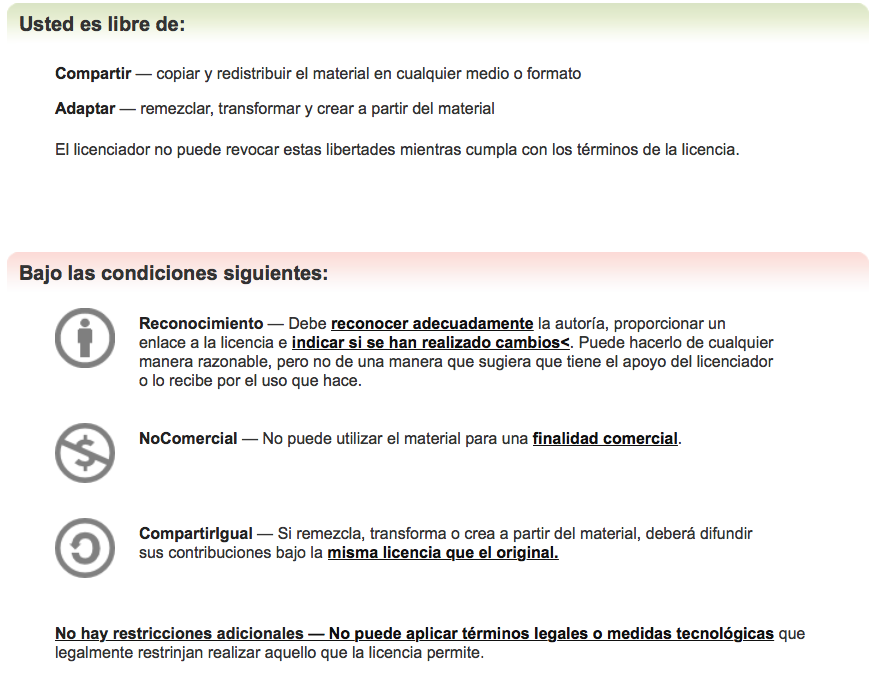
\includegraphics[scale = .4]{Figures/intro_img/attributions_esp.png}
\end{figure}
\begin{figure}[b!]
\centering

\includegraphics[scale = 2]{Figures/intro_img/by-nc-nd.pdf}
\end{figure}
\end{licence}


% Thesis Abstract -----------------------------------------------------


%\begin{abstractslong}    %uncommenting this line, gives a different abstract heading


\begin{resumen}        %this creates the heading for the abstract page
% Pon tu resumen aquí.

Escribir un resumen decente
 

\end{resumen}



%\end{abstractlongs}


% ---------------------------------------------------------------------- 

%: ----------------------- contents ------------------------

\setcounter{secnumdepth}{5} % organisational level that receives a numbers
\setcounter{tocdepth}{5}    % print table of contents for level 3
\tableofcontents
%: ----------------------- list of figures/tables ------------------------
\listoffigures

% \include{./src/Aknowledgments}
% \include{./src/Introduction}
% \include{./src/Problem}

% \include{./src/Electromagnetic_waves_in_periodic_media}
% \include{./src/Finite_element_method}
% \include{./src/Implementation}
% \include{./src/Results}
% \include{./src/Conclusions}



%: ----------------------- glossary ------------------------

% this file is called up by thesis.tex
% content in this file will be fed into the main document

% Glossary entries are defined with the command \nomenclature{1}{2}
% 1 = Entry name, e.g. abbreviation; 2 = Explanation
% You can place all explanations in this separate file or declare them in the middle of the text. Either way they will be collected in the glossary.
% required to print nomenclature name to page header
%\markboth{\MakeUppercase{\nomname}}{\MakeUppercase{\nomname}}

% ----------------------- contents from here ------------------------
%
\newacronym{OAM}{OAM}{Momento Angular Orbital - Optical Angular
Momentum}
\newacronym{VOs}{VOs}{Vórtices Ópticos - Optical Vortices (OV)}
\newacronym{LG}{LG}{Laguerre-Gauss}
\newacronym{SLM}{SLM}{Modulador Espacial de Luz - Spatial Light
Modulator}
\newacronym{LCD}{LCD}{Pantalla de Cristál Líquido - Liquid Crystal Display}
%\nomenclature{OAM}{Momento Angular Orbital - Optical Angular Momentum}
% \nomenclature{VO}{Vórtices Ópticos - Optical Vortices (OV)}
\newacronym{LCs}{LCs}{Cristales Líquidos - Liquid Crystals}
% \nomenclature{TN-LCD}{Pantalla de Cristál Líquido tipo Nemático Retorcido -Twisted Nematic Liquid Crystal Display}
% \nomenclature{RMS}{Error cuadrático medio - Root mean square}
% \nomenclature{AO}{Óptica Adaptativa - Adaptive Optics}
% \nomenclature{NI-WFS}{Sensado Remoto No Interferométrico - Non Interferometric Wavefront Sensing} 
% \nomenclature{PSF}{Función de Dispersión de Punto - Point Spread Function}
% \nomenclature{APSF}{Función de Punto Extendido de Amplitud - Amplitude
% Point Spread Function} 
% \nomenclature{FT}{Transformada de Fourier - Fourier Transform}
% \nomenclature{OTF}{Función de transferencia óptica - Optical transfer function}
% \nomenclature{GP}{Pupila Generalizada - Generalized Pupil}
% \nomenclature{AIV}{Armado, Integración y Verificación}
% \nomenclature{ESPI}{Interferometría de Patrones de Speckle Elecrónica}
% \nomenclature{SLM}{Modulador Espacial de Luz}
% \nomenclature{SH}{Shack-Hartmann}
% \nomenclature{LC}{Cristal Líquido}
% \nomenclature{CCD}{Dispositivo de Carga acoplada}
% \nomenclature{RMSE}{Error cuadratico medio}
% \nomenclature{SNR}{Coeficiente señal-ruido}
% \nomenclature{CTE}{Coeficiente de Expansión Térmica}
% \nomenclature{HDR}{Alto Rango Dinámico}
% \nomenclature{TVC}{Cámara de Termo-Vacío}
% \nomenclature{FEA}{Análisis de Elementos Finitos}
% \nomenclature{FEM}{Modelo de Elementos Finitos}
% \nomenclature{TUM}{Technische Universit\"{a}t M\"{u}nchen - Universidad Tecnológica de Munich }
% \nomenclature{OAM}{Momento Orbital Angular}
% \nomenclature{VCSEL}{Láser Emisor de Superficie de Cavidad Vertical}
% \nomenclature{WCOG}{Método de Compensación del Centro de Gravedad}
% \nomenclature{IWCOG}{Método Iterativo de Compensación del Centro de Gravedad}
% \nomenclature{FWHM}{Anchura Total a la mitad del Máximo}
% \nomenclature{SPT}{Transformada Espiral de Fase}
% \nomenclature{LK}{Método Lucas-Kanade}
% \nomenclature{LINES}{Laboratorio de Instrumentación Espacial}
% \nomenclature{INTA}{Instituto Nacional de Técnica Aeroespacial}
% \nomenclature{LCVR}{Retardadores Variables de Cristal Líquido}
% \nomenclature{FDT}{Full Disk Telescope - Telescopio de Disco Completo}
% \nomenclature{HRT}{High Resolution Telescope - Telescopio de Alta Resolución}
% \nomenclature{RFM}{Refocus Mechanism}
% \nomenclature{PHI}{Polarimetric and Helioseismic Imager}
% \nomenclature{BS}{Divisor de haz - Beam Splitter}
% \nomenclature{IAC}{Instituto de Astrofísica de Canarias}
% \nomenclature{GTC}{Gran Telescopio de Canarias}
% \nomenclature{ESA}{Agencia Espacial Europea}
% \nomenclature{PMP}{Polarization Modulation Package - Paquete de Modulación de la Polarización}
% \nomenclature{CMOS}{Semiconductor Complementario de Óxido Metálico}
% \nomenclature{APAN}{Nemático Antiparalelo - Anti-Parallel Nematic}
% \nomenclature{LBD}{Globos de Larga Duración - Long Duration Balloon}
% \nomenclature{NASA}{Administración Nacional de Aeronáutica y Espacio de USA - National Aeronautics and Space Administration}
% \nomenclature{GACE}{Grupo de Astronomía y Ciencias del Espacio}
% \nomenclature{IAA}{Instituto de Astrofísica de Andalucía}
% \nomenclature{FOV}{Campo de Visión - Field of View}
% \nomenclature{PSF}{Función de Punto Esparcido - Point Spread Function}
% \nomenclature{WFE}{Error del frente de onda - Wavefront error}
% \nomenclature{MTF}{Modulación de la función de transferencia óptica - Modulation Transfer Function}
% \nomenclature{PD}{Diversidad de Fase - Phase Diversity}
% \nomenclature{WHT}{William Herschel Telescope}
% \nomenclature{OGS}{Optical Ground Station}
% \nomenclature{FPGA}{Field-programmable gate array}
% \nomenclature{ENO}{Observatorios Europeos del Hemisferio Norte - European Northern Observatory}
% \nomenclature{AO}{Óptica Adaptativa - Adaptive Optics}
% \nomenclature{GS}{Método de Gerchgerg-Saxton}
% \nomenclature{SBMIR}{Single-beam Multiple-Intensity Reconstruction Technique}
%\nomenclature{ASD}{Descomposición espectral angular - Angular Spectrum Descomposition}

%\printnomenclature % [] = distance between entry and description
%Print the glossary
\label{sec:glossary} % target name for links to glossary
\printglossary[title=Lista de Acr\'onimos,toctitle=Lista de Acr\'onimos]



%: --------------------------------------------------------------
%:                  MAIN DOCUMENT SECTION
% --------------------------------------------------------------


% the main text starts here with the introduction, 1st chapter,...
\mainmatter
\pagestyle{fancy}

%: ----------------------- introduction ------------------------
% introduction

% this file is called up by thesis.tex
% content in this file will be fed into the main document

%------------------------------------------------------------------------- 

\chapter{Introducción}
\label{cha:Introduccion}

\graphicspath{{Figures/intro_img/}{../Figures/intro_img/}}

Como es bien sabido, la luz transporta energía; esto se hace evidente al
comparar las temperaturas en el día y en la noche o al iluminar una celda
fotovoltáica. En su representación cuántica, la luz está
compuesta por partículas sin masa llamadas fotones. Al no tener masa,
su energía está directamente asociada a su momento, y el momento de 
los fotones así como el de otras partículas en la mecánica cuántica puede ser tanto
lineal como angular. El momento angular se compone a su vez de dos
contribuciones, la de spin y la orbital. Desde un punto de vista 
macroscópico, el momento angular de spin se asocia con la polarización
de la luz, es decir con la dirección de oscilación de los campos
eléctrico y magnético con respecto a un eje coordenado. Asimismo, el
momento angular orbital (OAM) se asocia con las distribuciones
espaciales de la amplitud y la fase, tal y como se observan
en un plano perpendicular a la propagación de la luz. Para aclarar esta idea
comparemos dos haces polarizados linealmente, uno con OAM
cero, y el otro con OAM +1. El haz de luz que carece de momento
angular orbital presenta una distribución de fase constante. Si éste tiene una distribución de amplitud
Gaussiana, al ser enfocado por una lente, en un plano de
observación veremos que la distribución de intensidad está dada por una función de
Airy como la que se ilustra en la figura \ref{fig:oam_intro}c). 
%\ref{fig:oam0intro}  

lp;./['%\begin{figure}[h!]
%\centering
%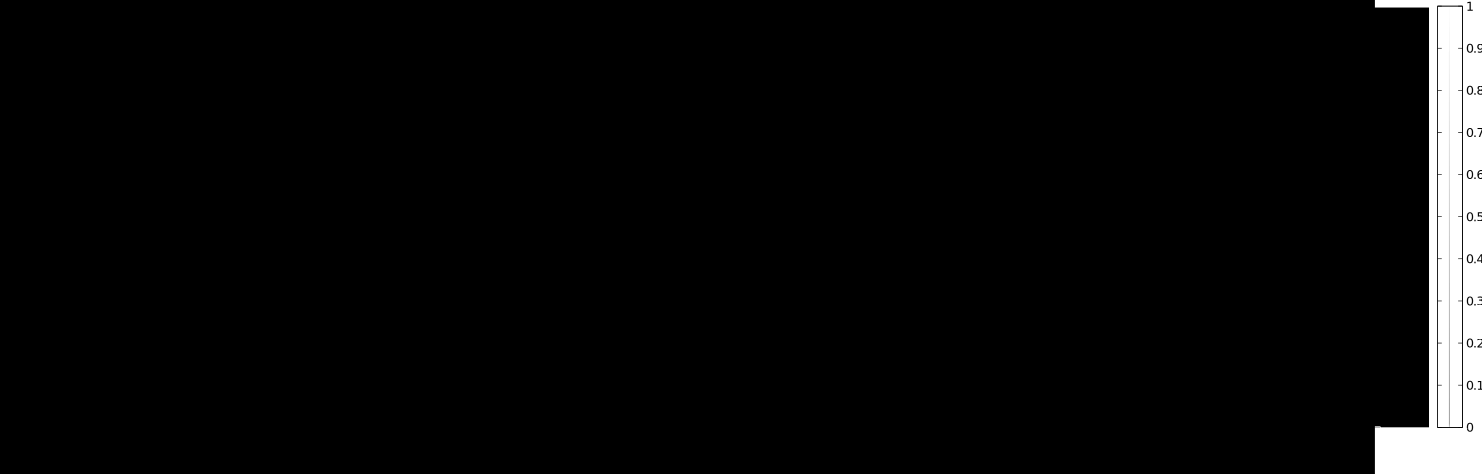
\includegraphics[scale=.33]{img/oam0Intro}
%\caption{a) Amplitud normalizada de un haz plano circular con OAM 0. b)
%Mapa de fase envuelta de $-\pi$ a $\pi$ radianes del mismo haz. c)
%Intensidad normalizada y corte transversal de un haz Gaussiano luego de
%ser enfocado.}
%\label{fig:oam0intro}
%\end{figure}

 Por el contrario, el haz con OAM +1 posee una distribución
 de fase helicoidal donde el valor de la fase varía azimutalmente
 desde $\pi$ a $-\pi$ radianes como se muestra  
en la  figura  \ref{fig:oam_intro}b). Haces con distribuciones de fase de este tipo poseen una
indeterminación de la fase en el centro dado que en la
coordenada $r=0$ confluyen fotones con todos los valores posibles de fase. La
consecuencia directa de la indeterminación en este tipo de puntos es
la ausencia de luz por efecto de superposición. Si, como en el caso
anterior, observamos la intensidad en un plano de enfoque veremos
perfil con forma de dona como la de la figura
\ref{fig:oam_intro} d). 


\begin{figure}[h!]
\centering
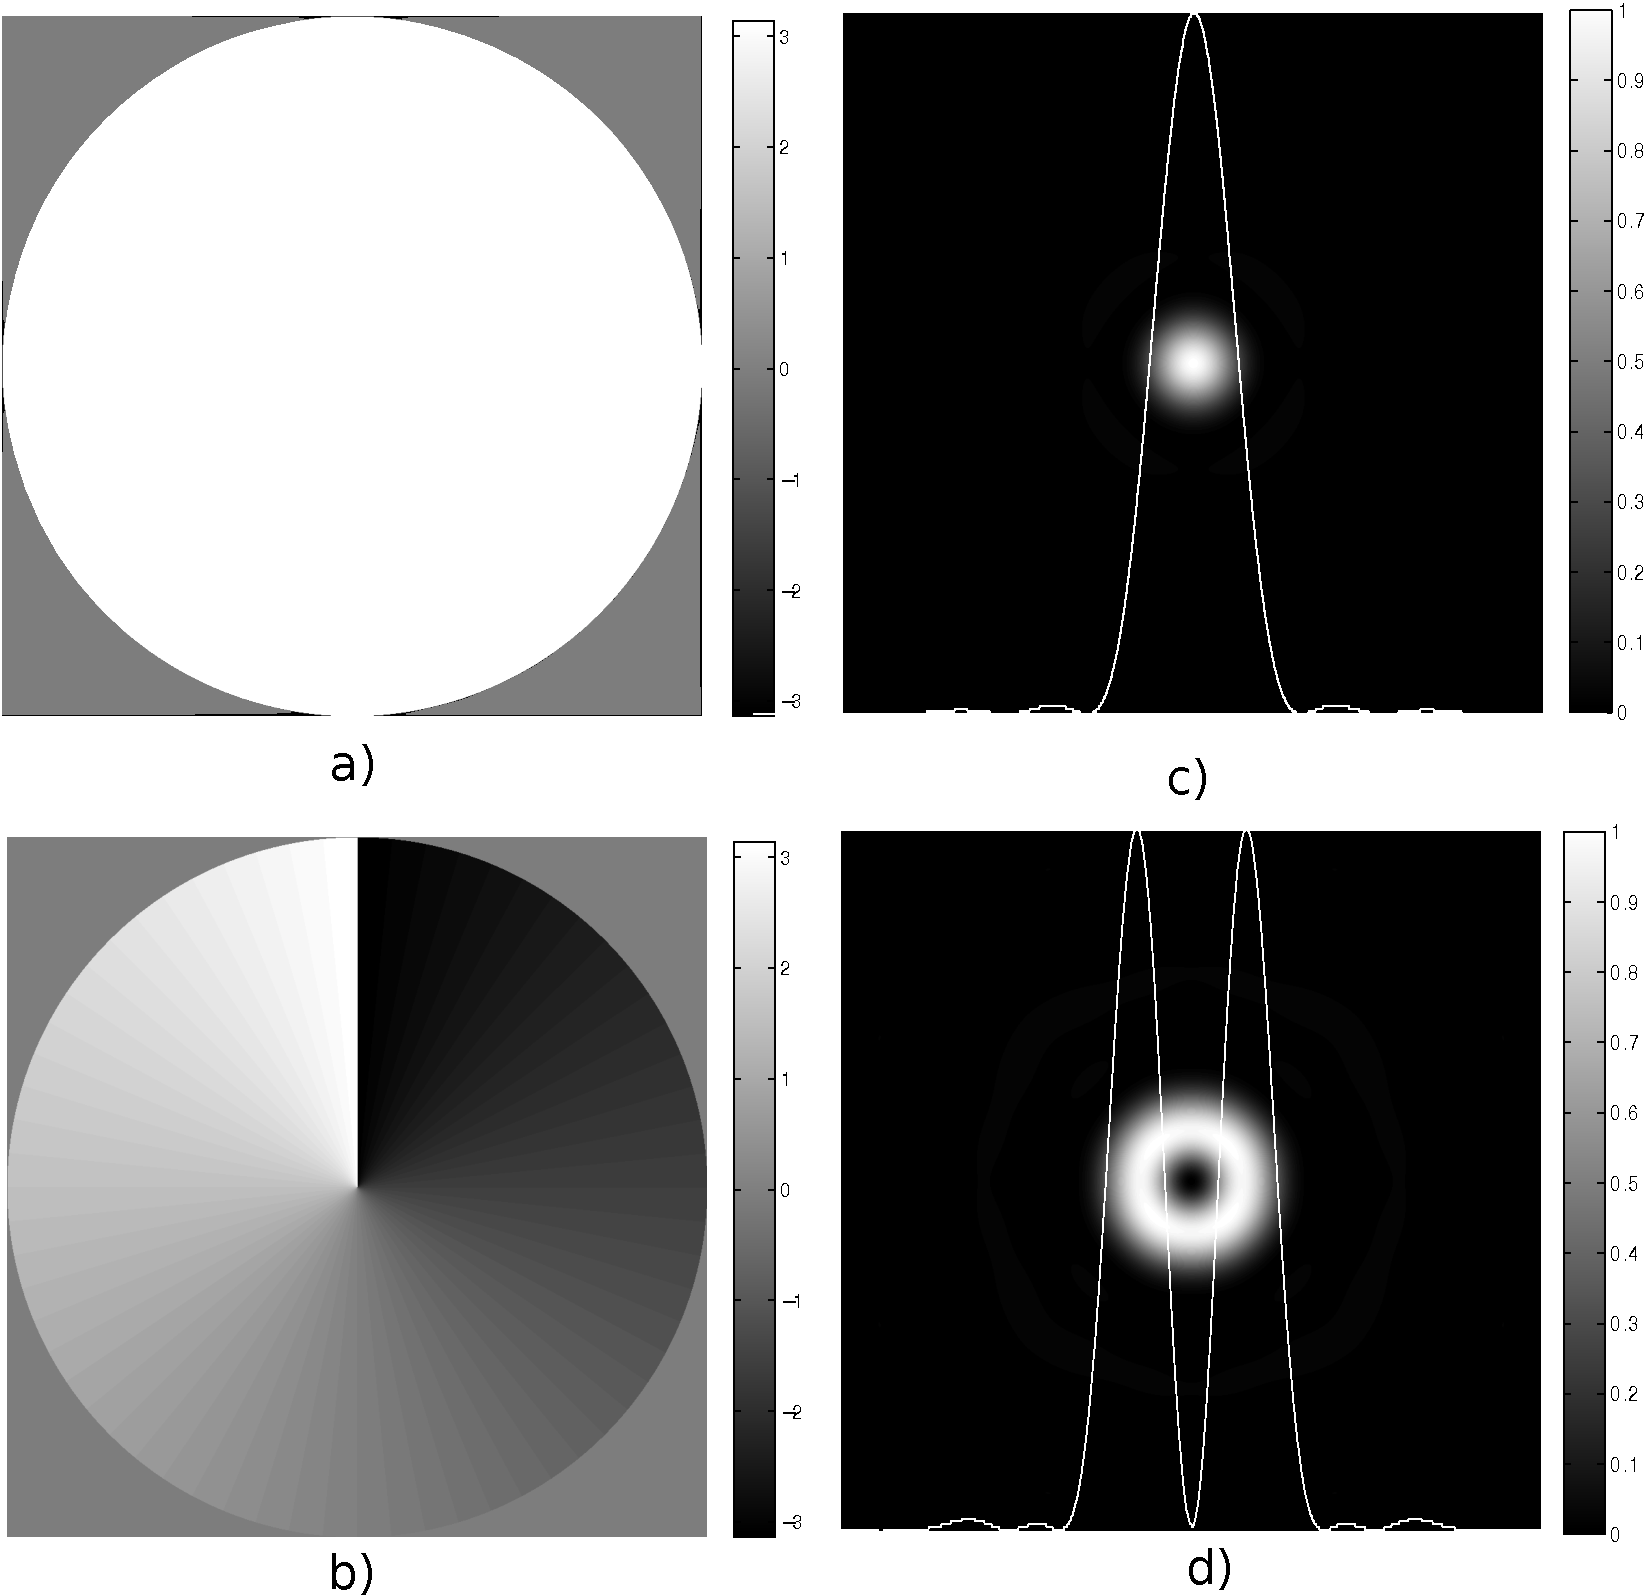
\includegraphics[scale=.33]{oam_Intro}
\caption{ Las figuras a) y b) representan mapas de fase de haces con
  OAM 0 y +1 definidos en el intervalo $[- 
  \pi,\pi]$ . Las intensidades correspondientes luego de enfocar los haces en
  un plano de observación se muestran en las figuras c) y d).}
\label{fig:oam_intro}
\end{figure}

Por su naturaleza rotacional, los puntos alrededor de los cuales la fase
varía de $-\pi$  a $\pi$ se conocen como \textbf{vórtices ópticos} (VO), y
están presentes siempre que haya haces con momento angular 
orbital distinto de cero. Por otra parte, de forma similar a cómo se
describe la amplitud en haces con OAM cero como ``Gaussiana'', 
los haces con momento angular distinto de cero se describen
matemáticamente como haces \textbf{``Laguerre-Gauss'' (LG)}. Esto se debe a que
soluciones de la ecuación de onda en coordenadas
cilíndricas incluyen no sólo una componente de amplitud Gaussiana, sino
también una dependencia radial y azimutal descrita por polinomios de
Laguerre, con los cuales se pueden representar vórtices ópticos de fase
y amplitudes del tipo dona.       
El estudio, y el desarrollo de aplicaciones sobre los haces Laguerre-Gauss y por consecuencia, de los VO , requiere entonces de la
capacidad de manipular el OAM de haces de luz.  \\

El momento angular orbital añade un grado de libertad al
conjunto de propiedades que pueden ser manipuladas y que caracterizan
a la luz, en particular: la polarización o espin, la coherencia, el
espectro y la cantidad de energía. Siendo así, la posibilidad de manipular el
momento angular orbital abre camino a un amplio rango de aplicaciones
en numerosas áreas de la ciencia y la tecnología, tanto en el mundo
microscópico (células y micromanipulación) como en el macroscópico
(astronomía y telecomunicaciones).  

Por listar brevemente algunas aplicaciones de los haces
con OAM distinto de cero se pueden mencionar: El uso de OAM en
telecomunicaciones ópticas como una nueva variable para 
multiplexación de señales en fibra y en espacio libre 
\citepInt{Lin2007,Gibson2004,Fontaine2012,Gibson2004,Bozinovic2013}. En microscopía
óptica para resaltar bordes de muestras biológicas transparentes \citepInt{Jesacher2005, Bouchal2012}, e identificar
curvaturas de objetos de fase por medio de interferometría espiral
\citepInt{Furhapter2005}. Además, es una herramienta esencial para la
manipulación de objetos en la escala micro al ser usados como pinzas ópticas capaces
de atrapar y mover partículas \citepInt{Grier2003}. Se espera también
un avance importante en el campo de la computación cuántica vía
entrelazamiento cuántico de OAM en fotones \citepInt{Mair2001}. Fuera de
las anteriores, cabe destacar algunas de las patentes relacionadas
con el tema como: aplicaciones en imagenología médica de resonancia magnética
n uclear \citepInt{Elgort}, y teledetección de objetivos militares
\citepInt{Schmitt}. También han sido patentadas herramientas y métodos
para micromanipulación de partículas microscópicas\citepInt{Grier}, con
posibles aplicaciones en bombas peristálticas para microfluidos
\citepInt{Guzzinati2014}. Para concluir, cabe mencionar  que hoy
en día la radiación óptica no es la única que está siendo usada  
para la propagación del momento angular orbital; destacan trabajos en
los cuales se utilizan los regímenes de ondas de radio
\citepInt{Thide2007}, rayos X \citepInt{Sasaki2008}, e inclusive haces de
electrones \citepInt{Guzzinati2014} para transmitir OAM. \\

Las referencias y ejemplos mencionados respaldan e ilustran el
intenso interés que se ha generado sobre el tema en la 
comunidad científica, y en particular en las áreas de óptica
aplicada y fotónica.  En Colombia, el tema de los vórtices ópticos es
un area  incipiente pero fértil. A nivel nacional se destaca una primera
iniciativa teórica por parte del grupo de óptica e información
cuántica de la  Universidad Nacional sede
Bogotá, en la cual se estudió la propagación de haces con OAM distinto de
cero en elementos ópticos conocidos como axicones
\citepInt{Guzman2009}. Asimismo, en el grupo de óptica y tratamiento de
señales de la Universidad Industrial de Santander han trabajado en el diseño de un codificador optoelectrónico
basado en el momento angular\citepInt{CristianAcevedo2012,Meza2013}. Es,
sin embargo en el ámbito regional de Antioquia en el cual se
concentra la mayor cantidad de esfuerzos en Colombia.  El grupo de
Óptica y Procesamiento Opto-digital de la Universidad 
Nacional sede Medellín desarrolló un sistema de pinzas ópticas para la
manipulación de microsistemas \citepInt{Alvarez2011}, mientras que el grupo de Óptica y Fotónica
de la Universidad de Antioquia ha estudiado la Multiplexación de
Información Encriptada y Codificación con Momento Angular
Orbital \citepInt{CarlosAndresRios2010}, así como la generación experimental de
vórtices ópticos con moduladores de transmisión
\citepInt{DavidMuneton2012,Rueda2013}. Además de los esfuerzos
de cada institución, destaca el trabajo colaborativo que se ha afianzado en el marco de convenios de
cooperación tales como el proyecto interinstitucional titulado:\\
\textit{Aberraciones ópticas en haces Laguerre-Gaussianos: corrección
  y aplicaciones metrológicas}. \\Este es un proyecto cuya duración es  de 24 meses, que
comenzó a ejecutarse el 5 de agosto de 2013 y que culminará el 5 de
agosto de 2015. Se desarrolla con la participación de grupos de la
Universidad EAFIT, la Universidad de Antioquia, el Centro de
Investigaciones Ópticas de Argentina, el Politécnico Colombiano Jaime
Isaza Cadavid, y el Instituto Tecnológico Metropolitano. 

De proyectos como este, se ha formado una red de grupos interesados
específicamente en el estudio de VO. En particular,
la cooperación entre algunos de ostos grupos derivó en trabajos en los
cuales se estudió el efecto de la birrefringencia inducida por
cristales birrefringentes en vórtices ópticos \citepInt{Gomez2012a}, y la
posibilidad de generar vórtices con una cantidad reducida de niveles
de gris en moduladores de transmisión \citepInt{Rueda2013}. De forma
similar, la Universidad EAFIT, a través de su grupo de Óptica Aplicada
y en cooperación con el Centro de Investigaciones Ópticas de
Argentina,  ha contribuido con el desarrollo de técnicas metrológicas
computacionales basadas en el estudio de  vórtices en patrones de
speckle
\citepInt{Angel-Toro2012,Angel-Toro2012a,Angel-Toro2013,Sierra-Sosa2013,Sierra-Sosa2013b}. 


Con la iniciativa de adquirir las capacidades técnicas y experimentales
necesarias para el desarrollo de aplicaciones metrológicas de vórtices ópticos, el grupo de Óptica
Aplicada de la Universidad EAFIT ha abierto dos proyectos internos, y
ha sido merecedor de una beca del programa Jóvenes Investigadores de Colciencias,
convocatoria 645 a cursar en el 2015.  
Las prioridades del grupo, y asimismo los temas de trabajo de estos
dos proyectos son: 
\begin{itemize}
\item El desarrollo de aplicaciones metrológicas de haces Laguerre
  Gauss. 
\item La implementación de técnicas basadas en los haces con OAM
  distinto de cero para instrumentos de microscopia de objetos de fase. 
\end{itemize}

Es, en este contexto, que desde Julio del 2013 he venido realizando mi labor de
investigación en la línea de metrologia óptica del grupo de Óptica Aplicada de la Universidad EAFIT
en el proyecto interinstitucional  \textit{Aberraciones ópticas en haces Laguerre-Gaussianos: corrección
  y aplicaciones metrológicas} gozando del beneficio de un beca de Maestría. 

% % duración del programa. Así como realizar mi trabajo de grado en armonía con
% % el mismo. 

% %Este trabajo se plantea como un desarrollo complementario de la línea
% %de investigación del grupo en la cual he venido trabajando

Mediante la presente propuesta de Trabajo de Grado se busca proponer
un proyecto final de maestría con el cual se pueda concluir y documentar
un proceso académico e investigativo de dos años que va a permitirle al
grupo de Óptica Aplicada abrir nuevas areas de trabajo. 
Específicamente, se propone terminar de desarrollar las capacidades técnicas y
habilidades necesarias para la manipulación del OAM y la generación de
VO con miras a la exploración de nuevas aplicaciones de VO en la
metrología óptica y la microscopía. \\


En adelante, en la sección \ref{sec:planteamiento} se presentará el
planteamiento del problema. En la sección \ref{sec:marco_teorico}, se presentará  un breve marco
teórico y estado del arte que dará soporte a las proposiciones del planteamiento del problema.
% Adicionalmente se abordará una breve sección
% de análisis de riesgos (\ref{sec:analisis}) en la cual se pretende evaluar las posibles
% limitaciones y fuentes de retraso o aplazamiento. 
Y en la sección \ref{sec:objetivos} se presentará el objetivo general y enumerarán
los objetivos específicos que deben ser cumplidos al finalizar el
proyecto. Luego, en la sección \ref{sec:metodologia} se hará una descripción de las
actividades a realizar para la consecución de los objetivos
específicos, y se presentará un cronograma (sección \ref{sec:cronograma})  que
establece los tiempos en los cuales se deben cumplir. Finalmente, se
presenta una descripción de los recursos necesarios
para llevar a cabo el proyecto y se listan las referencias
bibliográficas consultadas. 

\section{Motivación y objetivos\label{sec:motiv}}


%------------------ESTADO_DEL_ARTE---------------
\section{Estado del Arte\label{sec:estadoArte}}




%-----------------ESTRUCTURA-------------------
\section{Estructura\label{sec:estructura}}

El texto principal de este trabajo, está dividido en 2 partes temáticas que agrupan los Capítulos. A continuación, se presenta la estructura general de la disertación por Partes y Capítulos: \\


\textbf{Parte \ref{ParteI}: Implementación de una plataforma para la caracterización de un SLM}



\textbf{Parte \ref{ParteII}: Caracterización y corrección de aberraciones de VO}


\textbf{Parte \ref{ParteIV}: Recuperación de fase con métodos no interferométricos}


\newpage
\pagebreak[4]
\bibliographystyleInt{unsrtnat}
\bibliographyInt{References/Int}






	
%\include{1_introduction/1_motivation}	

%: ----------------------- Parte I ------ ------------------------

\part{Generación de haces Laguerre-Gauss por medio de un SLM\label{ParteI}}

% this file is called up by thesis.tex
% content in this file will be fed into the main document

%------------------------------------------------------------------------- 

%\chapter{Generación de Vórtices Ópticos}
\chapter{Generalidades y Marco Teórico}
\label{cha:Gen_intro}

\graphicspath{{Figures/ch2_img/}{../Figures/ch2_img/}}
\lhead{Generación de haces Laguerre-Gauss por medio de un SLM: \textit{Introducción}} % This is for the header on each page - perhaps a shortened title

\section{Estado del Arte} %Introducción????
\label{sec:ChGen_estado_del_arte}
\lhead{Generación de Vórtices Ópticos: \textit{Estado del Arte}}
Los haces con \acrshort{OAM} distinto de cero inicialmente fueron generados en el
laboratorio por medio de técnicas analógicas entre las que se destacan
el uso de conversores modales \citepChGen{Alekseev1998}, placas de fase espiral grabadas en sustratos
transparentes \citepChGen{Jun2009}, y hologramas de fase impresos en acetato
\citepChGen{Carpentier2008} . La conversión modal utiliza sucesiones de
lentes astigmáticas para convertir los modos Hermite Gauss en modos
Laguerre-Gauss, y fue la primera forma en la cual se produjeron VOs en
el laboratorio. A diferencia de la conversión modal, - que requiere un
montaje experimental muy sensible a desplazamientos -  las técnicas que utilizan máscaras
de fase se caracterizan por necesitar sólo un elemento óptico que
permite modificar punto a punto la fase de un haz que originalmente
carecía de momento angular, para convertirlo en un haz con vorticidad
óptica. El uso de placas físicas grabadas con un patrón espiral
tiene la ventaja de generar haces LG con sólo ubicarlas en
el camino óptico del haz, y tiene la desventaja de que una vez
fabricadas no se pueden modificar. 
En situaciones donde es requerido generar haces del tipo LG con la suficiente
flexibilidad como para corregir aberraciones ópticas, se
necesita de dispositivos digitales con propiedades similares a los
dispositivos analógicos mencionados anteriormente. Estos dispositivos
se conocen como moduladores espaciales de luz o SLM por sus siglas en
inglés. En este proyecto se pretende generar VOs y caracterizar su
frente de onda utilizando un tipo de SLMs que modifican la fase de la
luz cuando ésta pasa a través de ellos. 

\subsection{Moduladores Espaciales de Luz}

Como su nombre lo indica, los moduladores espaciales de luz sirven
para modular punto a punto las propiedades de la luz sobre un
plano. Ya sea solamente su amplitud como en los dispositivos de
visualización de cristal líquido (pantallas \acrshort{LCD}), o su fase, como en
los dispositivos que se ilustran en la Fig.~\ref{fig:LCDSLM}.
\begin{figure}[h!]
\centering
    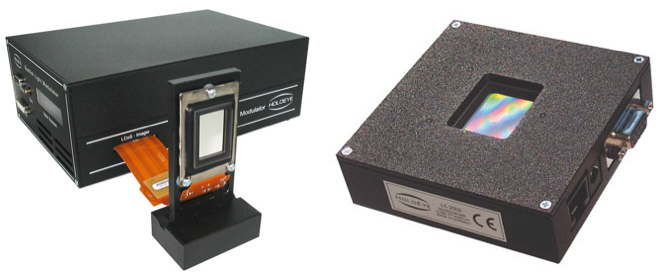
\includegraphics[width=0.5\textwidth]{LCDSLM.png}
\caption[Comparación entre TN-SLM]{Moduladores espaciales modelo PLUTO y LC2012 de reflexión y
  transmisión marca Holoeye basados en la tecnología de cristal
  líquido.}% Por ser fabricado a partir de un LCD comercial el modulador de  la derecha es ensamblado a una cuarta parte del costo del izquierdo.}
\label{fig:LCDSLM}
\end{figure}

Si diferenciamos los SLM por el tipo de tecnología, estos pueden ser
agrupados en dos categorías: basados en cristales líquidos, o en
arreglos de micro espejos (Fig.~\ref{fig:MEMSLM}), mejor 
conocidos en la industria de la proyección como DLP (de Digital Light
Processing).  
\subsubsection{Moduladores basados en micro espejos}
En su mayoría, los moduladores comerciales basados en arreglos de micro
espejos funcionan con micro mecanismos que inclinan una superficie
reflectiva de tal forma que se modifique la cantidad de luz que un
observador ve desde una perspectiva dada, es decir que modulan
intensidad. Sin embargo, con el interés de modular fase además de
intensidad se han desarrollado nuevos micro mecanismos que
permiten desplazar verticalmente el espejo sin modificar su
inclinación, introduciendo así un cambio en la distancia del camino
óptico y por ende, la fase. Tal y como se presenta en los trabajos de
\citetChGen{Wu2010} y \citetChGen{Liesener2006}. Dado que es una
tecnología incipiente y ha tenido menor tiempo en el mercado que los
cristales líquidos, estos sistemas de micromecanismos y en particular los de tipo pistón,
siguen teniendo precios elevados y aún están lejos de ser utilizados
en muchos laboratorios. 
\begin{figure}[h!]
\centering
    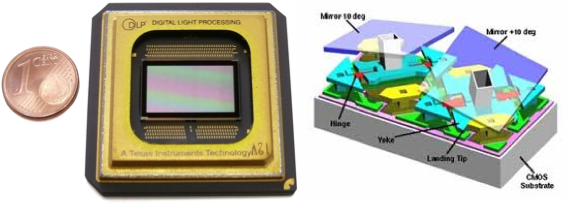
\includegraphics[width=0.5\textwidth]{MEMSLM.png}
\caption[Modulador espacial basado en arreglos de micro espejos]{Modulador espacial basado en arreglos de micro espejos marca Texas Instruments.}
\label{fig:MEMSLM}
\end{figure}

\subsubsection{Moduladores de cristal líquido}
Los SLM basados en Cristales Líquidos (\acrshort{LCs}) aprovechan las propiedades
físicas de ciertos polímeros que dada su forma alargada y propiedades
electrónicas polares, cambian su orientación ante la presencia de
campos eléctricos.  Esta sensibilidad a los campos eléctricos, en
conjunto con sus propiedades ópticas anisotrópicas permitió que desde
los años 70s se implementaran LCs para generar imágenes en pantallas de
dispositivos como relojes, calculadoras y luego televisores y
proyectores. Fue más adelante cuando estudios especializados de las
propiedades de los LCs como los realizados por
\citetChGen{Yeh1999} y \citetChGen{Yariv2002}, y experimentos como los de
\citetChGen{Konforti1988} demostraron que los LCD pueden ser usados
como moduladores de solo fase. Aunque la aplicación de LCs para
modulación de fase es relativamente reciente, el estudio de sus
propiedades físicas no lo es y desde los años 60’s la investigación ha
sido respaldada por grandes empresas interesadas en desarrollar
productos tecnológicos de generación y procesamiento de imágenes como
RTC, Hamamatsu, Hitachi, HP, Texas Instruments, Sony y otros. Dado
el interés por entender los LCs, se ha llegado a modelos matemáticos y  técnicas de  
caracterización robustas que permiten extraer los parámetros de un SLM para
 simular su comportamiento. 
El desarrollo de estas técnicas ha permitido a investigadores 
alrededor del mundo implementar moduladores de fase a
partir de elementos LCD extraídos de dispositivos de proyección
comerciales, entre ellos se encuentran los trabajos de
\citepChGen{Pezzaniti1993,Soutar1994,Zhang1994,Moreno1998,Davis1999,Iemmi2001,Davis2003,Moreno2003,Kim2005,Duran2006,Duran2007,Marquez2007,Liu2010,Ma2010,Ma2011,Yu2012}. Mientras
que autores como Mahmud, \citepChGen{Mahmud2008}, Roopahsree
\citepChGen{Roopashree2009a}, y David \citepChGen{Dev2012}
caracterizaron un Holoeye LC2002 que es vendido comercialmente como
modulador de amplitud y fase.
Ejemplo de la práctica de reensamblar un LCD y venderlo como SLM es el
modulador marca Holoeye LC2012 que gracias a usar un LCD comercial
marca Sony es ensamblado a una cuarta parte del precio de otros
moduladores. 

Adicionalmente, cabe mencionar que los moduladores en base a LCs se
dividen en dos tipos, de reflexión y de transmisión. Sin entrar en
detalle, los primeros permiten modulaciones de fase que van hasta $2\pi$
radianes, tienen mayor resolución, necesitan menos elementos de
polarización para su uso, tienen altas velocidades de operación y el
hecho de que la electrónica esté detrás del cristal (y detrás de la
superficie reflectiva) hace que se produzcan menos efectos indeseados
de difracción. Todo esto a costa de desarrollar LCs y
electrónica personalizados. En cambio, los moduladores de transmisión
se ensamblan a partir de LCs comerciales que fuera de polarizar la luz
retardan su fase. Esto implica un acople entre modulación de fase y 
modulación de intensidad que se traduce en menor calidad de la
modulación de fase total. Para lograr una modulación específica se
necesitan polarizadores y retardadores que generen un 
estado de polarización particular a la entrada del SLM. Por otra
parte, al tener la electrónica acoplada sobre el cristal y no en un
elemento separado como en los de reflexión, se limita la
resolución; no todo el volumen de LC se aprovecha y se introducen
efectos indeseados de difracción. 
No obstante, los SLM de transmisión son muy económicos y algunos
autores como Davis et al. \citepChGen{Davis2000, Davis2013} han propuesto
que se podrían usar como dispositivos para modular polarización. En
base a la idea de usarlos para modular polarización, otros como \citetChGen{Moreno2004, Moreno2011} han
combinado el formalismo de Fourier con el de las matrices de Jones
para modelar el comportamiento de dispositivos ópticos de Fourier que
involucran polarización. 

En el laboratorio de metrología óptica del grupo de Óptica Aplicada de
la Universidad EAFIT se encuentra un moduladores de transmisión
marca Holoeye modelos LC-2002 que en el contexto de este
trabajo ha sido caracterizado para optimizar su uso en aplicaciones metrológicas
tales como la creación y corrección de aberraciones en haces LG.  
La generación de VOs se da entonces de forma expedita una vez se tenga apropiada la
herramienta que los produce.  
A lo largo de este capítulo se presentarán los conceptos teóricos
necesarios para entender la caracterización de SLMs y luego se
presentarán las diversas herramientas y métodos que se implementaron
para lograr la generación de VOs.

% En la sección que sige se introduce la segunda mitad del
% problema, es decir, ¿Cómo caracterizar y corregir las aberraciones ópticas de un VO?

% \subsection{Aberraciones ópticas}

% Los VO generados en el laboratorio están sujetos a aberraciones
% ópticas que se asocian a situaciones tales como:
% \begin{itemize}
% \item Problemas en la alineación de componentes ópticos como
%   lentes o espejos.
% \item Deformaciones en las superficies de elementos como
%   polarizadores, lentes, espejos, láminas retardadoras, e incluso de
%   las céldas de cristal líquido en el SLM.
% \item Presencia de partículas de polvo en las superficies de las
%   componentes ópticas que inducen efectos indeseados de difracción. 
% \end{itemize}

% Adicionalmente, y siguiendo con el tema de la sección anterior, los
% SLM de transmisión basados en pantallas de LC introducen otras fuentes
% de aberraciones. En primera medida, los LCD son dispositivos discretos en dos de los
% sentidos de la palabra; por un lado, son discretos espacialmente y
% las señales de control son asignadas a subdivisiones del cristal de tamaño finito
% conocidas como píxeles. El arreglo rectangular de todos los píxeles
% genera efectos de difracción similares a los de rejillas verticales y
% horizontales combinadas. Esto quiere decir que el SLM separa los
% órdenes de difracción de la luz que pasa a travez de él. Asimismo, el
% hecho de ser una cuadrícula discreta hace que el modulador no pueda
% generar distribuciones de fase en regiones infinitamente pequeñas como
% sería deseado alrededor de una singularidad óptica. Como ejemplo, en la figura
% \ref{fig:discrete_mask} a) se muestra una imagen de la región donde
% resultaría una singularidad óptica en una máscara de
% fase espiral enviada al SLM. Como se puede ver, la máscara de fase
% discreta resulta muy distinta a la máscara ideal presentada en la
% figura \ref{fig:oam_intro}b), y por lo tanto introduce deformaciones
% en el haz Laguerre-Gauss que resulta a la salida del SLM.   

% \begin{figure}[h!]
% \centering
% 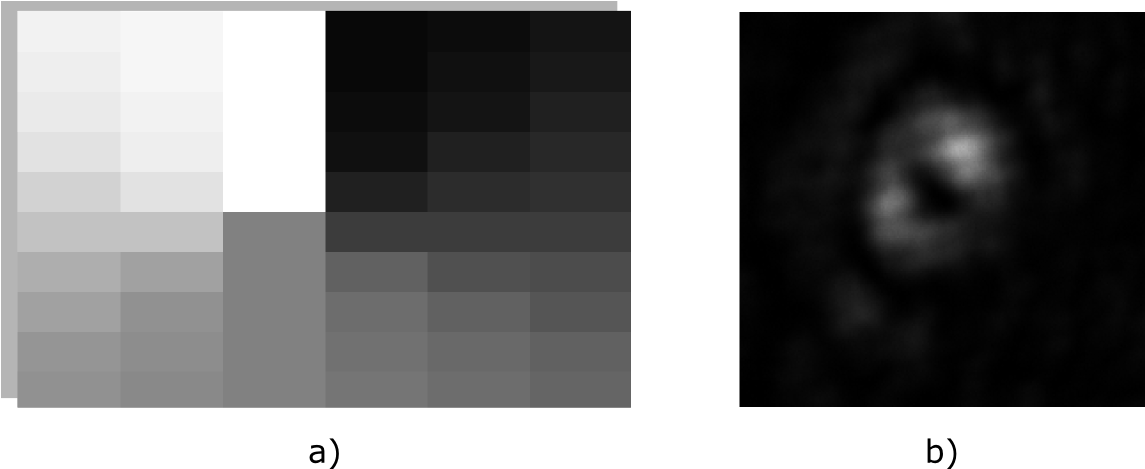
\includegraphics[ scale=.4]{discrete_mask.png}
% %Las imagenes que enviamos al SLM son generadas en un
% %  ordenador que de por sí es discreto, y llegan a un dispositivo
%  % físico que tiene divisiones discretas, tanto espaciales como
%  % electrónicas. Aún 
% \caption[Efecto de pixelado eb el SLM sobre las aberraciones en VO]{a) Magnificación de una mascara tipica proyectada al SLM. b) Imagen de un VO de poca calidad producido con un SLM de
% transmisión modelo Holoeye LC2002.}
% \label{fig:discrete_mask}
% \end{figure}

% Por otra parte, el SLM es discreto en la medida que sólo puede asignar
% níveles de voltaje discretos (0-255 divisiónes de 5V) a cada una de
% las celdas. Este fenómeno también es observable en la figura
% \ref{fig:discrete_mask}a) y puede introducir efectos
% indeseados. Más aún, si cómo el nuestro, el modulador no llega a una
% modulación de sólo fase, o tiene una modulación que no llega a
% completar el ciclo de $2\pi$ radianes. 
% Todas las posibles fuentes de error mencionadas anteriormente se
% combinan para generar haces Laguerre-Gauss de poca calidad como el que se muestra
% en la figura \ref{fig:discrete_mask} b). 


\section{Marco Teórico de la Caracterización de SLMs de Trasmisión}
\label{sec:ChGen_marco_teorico}
\lhead{Generación de haces Laguerre-Gauss por medio de un SLM: \textit{Marco Teórico}}

Dado que los SLMs de transmisión se ensamblan a partir de LCs, lo
primero que hay que tener en cuenta para su caracterización 
es conocer sus generalidades y entender sus propiedades ópticas. 
Entenderemos que los LCs afectan el estado de polarización de la luz y
por ello se dedicará un espacio del marco teórico a presentar los conceptos
generales y herramientas matemáticas propias de la teoría de polarización. 
Una vez presentadas estas herramientas se mostrarán los modelos
actuales con los cuales se representa matemáticamente la modulación de
un LC y se hará una breve revisión de la literatura de la
caracterización de SLMs. 

\subsection{Cristales líquidos}
\subsubsection{Características de los Cristales Líquidos}  
Un cristal Líquido es una sustancia que posee propiedades que
se asemejan tanto a las de los sólidos cristalinos como a las de los
líquidos, y puede ser visto como un líquido en el cual existe
orden entre sus moléculas. Para ilustrar esta idea recordemos que los
sólidos cristalinos son un estado de la materia que se caracteriza por
su rigidez y fuertes enlaces químicos, en el cual se puede
establecer un orden posicional en todas las direcciones tal y como se
ilustra en la Fig.~\ref{fig:solido}. Esto implica que la posición de
las moléculas o átomos que lo componen puede ser abstraída como una
red periódica que cumple ciertas reglas de simetría. En cambio, un
líquido amorfo como el de la Fig.~\ref{fig:liquido} tiene enlaces
más débiles por lo cual puede fluir y está compuesto
por moléculas que están completamente desorganizadas. 
\begin{figure}[h!]
\centering
\begin{subfigure}{.45\textwidth}
  \centering
  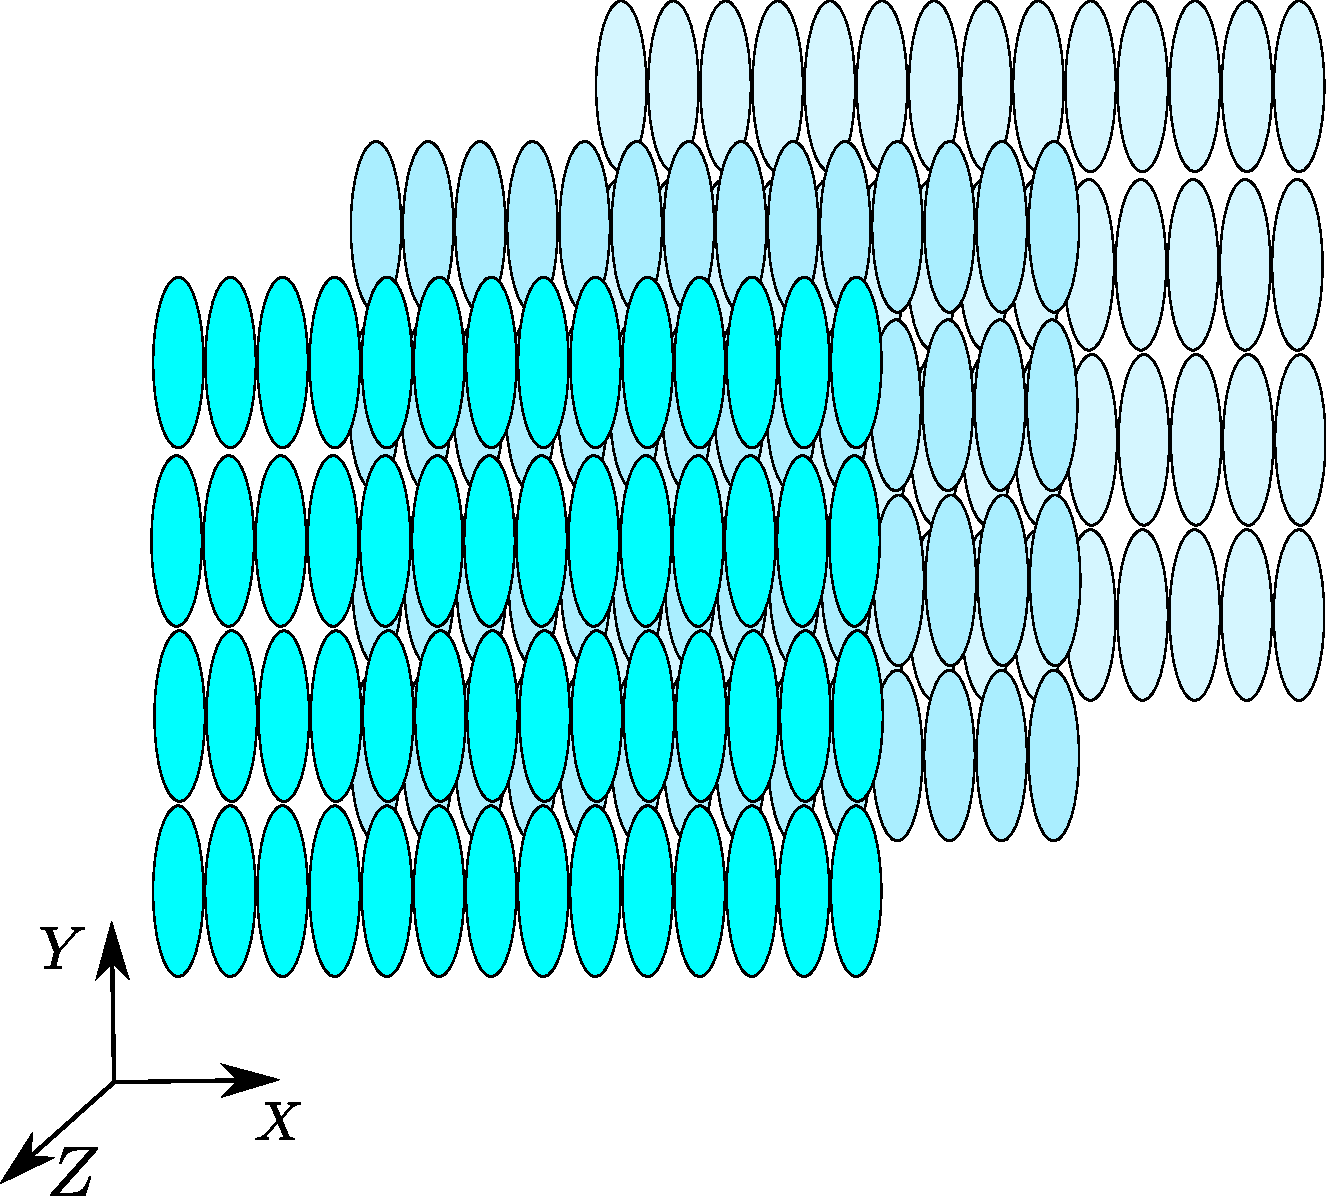
\includegraphics[width=.6\linewidth]{Cristaline_solid}
  \caption{Moléculas con orden posicional y orientacional en un sólido cristalino.}
  \label{fig:solido}
\end{subfigure}\qquad
\begin{subfigure}{.45\textwidth}
  \centering
  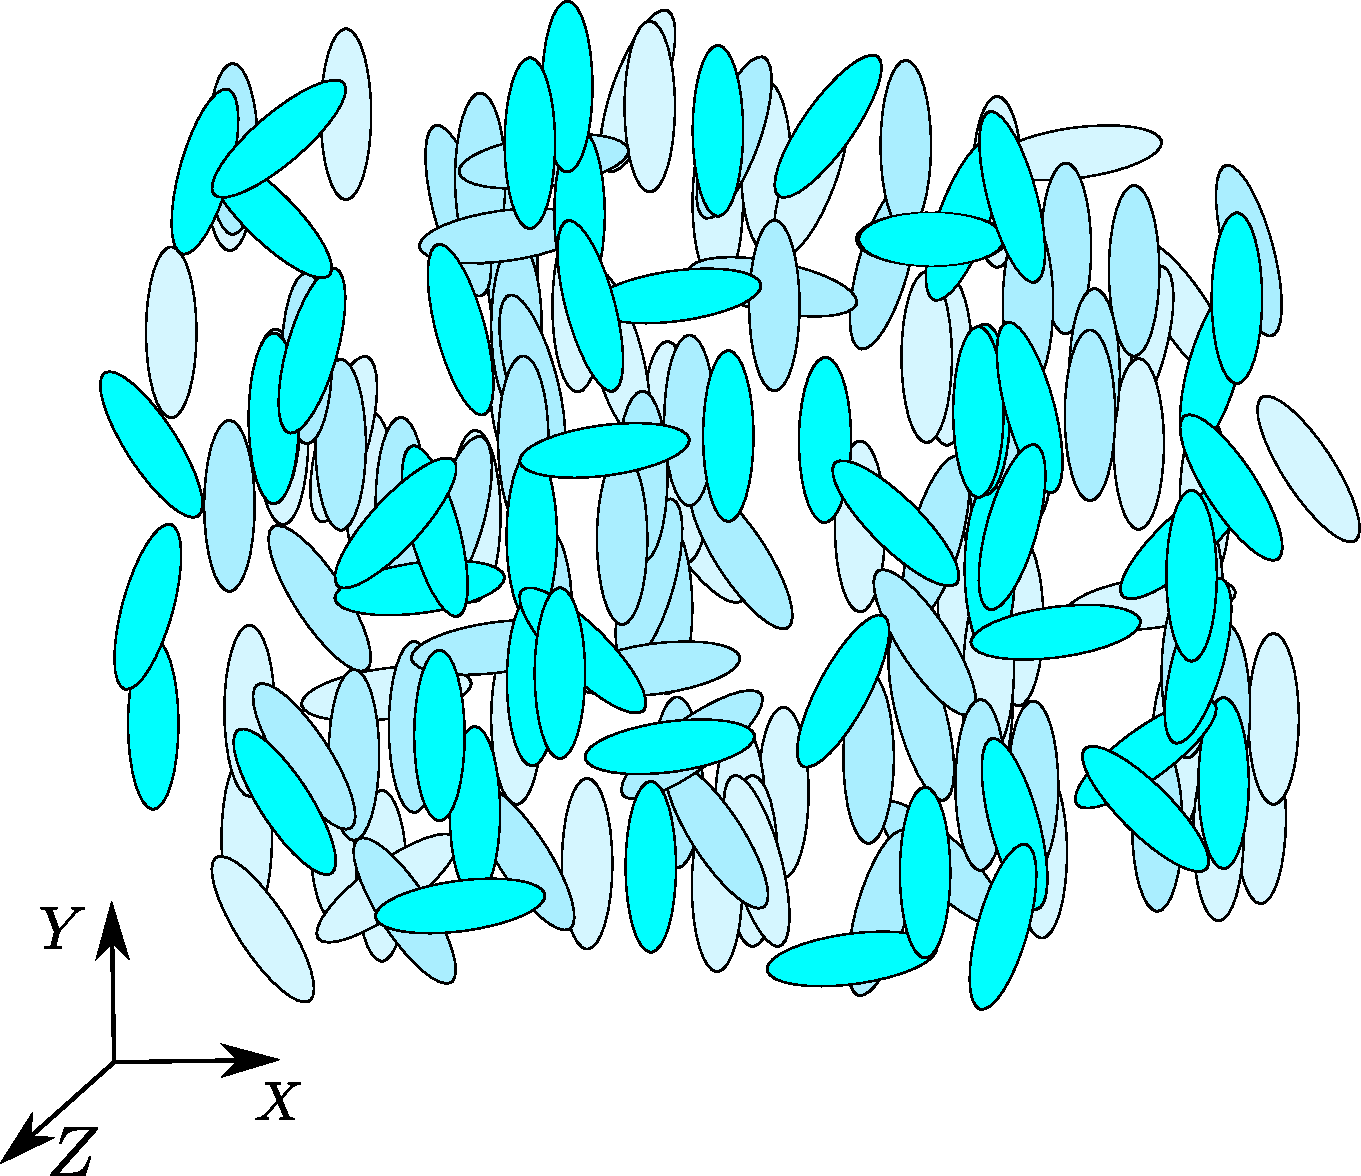
\includegraphics[width=.6\linewidth]{liquid}
  \caption{Moléculas desordenadas pero cercanas en un líquido.}
  \label{fig:liquido}
\end{subfigure}
\caption{Dos estados de la materia comunes en la naturaleza.}
  \label{fig:estados}
\end{figure}

Los cristales líquidos son sustancias que como los
sólidos poseen cierto orden y que pueden fluir como los líquidos. 

Por otra parte, los LCs pueden ser clasificados en tres tipos o fases distintas
conocidas como, \textit{nemáticos},
\textit{smeticos} y \textit{colestéricos}, y más adelante se abordará esta
clasificación. No obstante su diversidad (más de 100.000 compuestos
distintos según \url{http://www.lci-publisher.com}), la característica
común de los LCs es que están 
compuestos de moléculas altamente anisotrópicas, esto es, que sus
propiedades (ópticas, eléctricas y mecánicas) dependen de la
dirección desde la que se observen. La anisotropía se debe tanto a la
geometría alargada o achatada de las moléculas, como a las propiedades
electrónicas de sus componentes \citepChGen{Gennes1995,Yeh1999,Yariv2002}. En el caso de moléculas
alargadas de LCs como la de la Fig.~\ref{fig:LCMolecule} la
estructura química de un LC general se
compone de un sistema de anillos aromáticos que pueden ser o no
saturados conectados por un grupo de conexión A, y sujetos a dos
cadenas o grupos terminales X y Y \citepChGen{Yeh1999}. 
\begin{figure}[h!]
\centering
    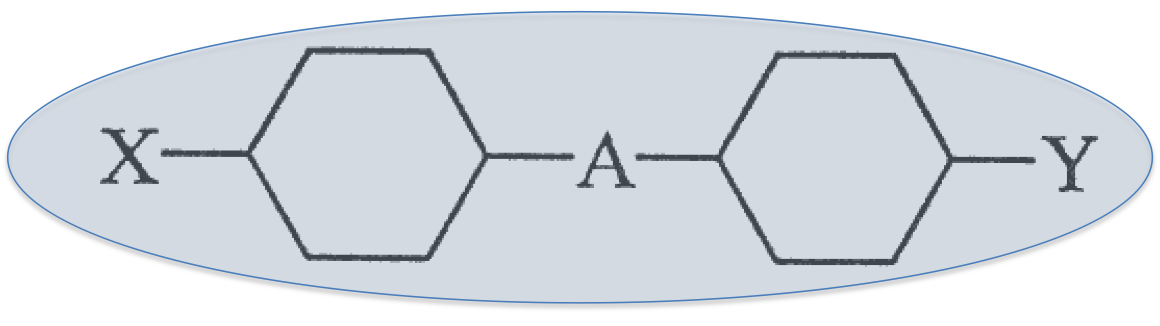
\includegraphics[width=0.5\textwidth]{LCMolecule}
\caption{Esquema de la composición química general en una molécula de LC.}
\label{fig:LCMolecule}
\end{figure}

La presencia de los anillos proporciona las fuerzas intermoleculares de corto alcance que
son necesarias para formar fases nemáticas y el tipo de anillos
(saturado o no saturado) determina la presencia o no de enlaces $\pi$
que se asocian a orbitales $P_z$ de los electrones. Esto a su vez
afecta la absorción en el ultravioleta y la birefringencia; se observa mayor
birefringencia en LCs con anillos no saturados y mejor comportamiento
en el ultravioleta para anillos saturados \citepChGen{Gennes1995}.  Luego, las cadenas del
grupo terminal X pueden ser de tres tipos,
\begin{itemize}
\item Cadenas alquilos (alkyl)  $C_nH_{2n+1}$,
\item Grupos alcoxy $C_nH_{2n+1}O$,
\item Grupos alilos (alkenyl) $CH_2=CH-CH_2-$.
\end{itemize}
 La longitud de las cadenas X influencia tanto las constantes elásticas
 como las temperaturas de transición de fase. Para cadenas cortas con
 uno o dos átomos de carbono los grupos son muy cortos como para
 presentar fases de LC. Los grupos terminales de tamaño medio: n = 3-8
 son los más adecuados para construir fases nemáticas por su
 mayor anisotropía, y los compuestos con cadenas aún más largas
 exhiben fases smeticas. La temperatura a la cual la solución pasa de
 ser nemática a isotrópica se conoce como el punto de aclarado o
 \textit{clearing point}, en términos generales, esta temperatura
 disminuye en la medida en la que se alargan los tamaños del 
 grupo terminal X. La función que relaciona el punto de aclarado con
 el número de átomos de carbono es una función suave en la cual los
 números pares generan temperaturas más bajas que los impares. Fuera
 de esto, las propiedades mecánicas como la viscosidad también se ven
 afectadas por el tamaño de los grupos terminales, cadenas
 largas implican viscosidades más altas, y por ello frecuencias de
 operación más bajas \citepChGen{Gennes1995}. 
Finalmente, las cadenas que forman el grupo terminal Y son las que
tienen mayor influencia en las constantes dieléctricas de la molécula
($\epsilon_x,\epsilon_y$), y asimismo su anisotropía dieléctrica
$\Delta\epsilon$ variables que como veremos más adelante son las que
determinan la birrefringencia del LC asociada a la modulación de fase.
Las cadenas del grupo terminal Y pueden ser:
\begin{itemize}
\item No polares: No Influencian mucho la anisotropía dieléctrica, un
  ejemplo es el grupo alquilo $CnH2n+1$.
\item Polares:  Como CN, F, y Cl. Su alta polaridad induce en la
  molécula una alta anisotropía dieléctrica y por tanto alta
  birrefringencia. La alta anisotropía se obtiene a costa de alta viscosidad, resistividad
  insuficiente y problemas de estabilidad bajo iluminación 
  ultravioleta. Los grupos Y muy polares como los que contienen
  cianuro CN No son buenos para operar a  altas temperaturas como por
  ejemplo proyectores, y sufren de degradación en el UV. Para esas
  aplicaciones se utilizan compuestos menos polares como el flúor o
  cloro que tienen menor birrefringencia \citepChGen{Gennes1995}.
\end{itemize}

\subsubsection{Clasificación de los LC}  
\label{sec:LC-clasification}
En 1922 y sintetizando los hallazgos de 30 años desde el descubrimiento
de los LCs, el cristalógrafo George Friedel publicó un artículo \citepChGen{Friedel1922}
en el que clasifica los LCs en tres tipos básicos conocidos como
cristales smeticos, nemáticos y colestéricos.
En términos de orden, los LCs sméticos son los más similares a un
sólido, y los nemáticos se asemejan más a un líquido, y en la medida
en la que se calienta un LC éste realiza una transición desde cristal
smetico hasta líquido isotrópico pasando por la fase nemática. Los estados
colestéricos son un tipo particular de LCs nemáticos que a diferencia
de los anteriores tienen propiedades inhomogeneas. 
La principal característica que le da una medida de orden a los LCs es
la tendencia de sus moléculas a orientarse en una dirección
preferente gracias a su distribución polar de cargas. Esta tendencia
se puede observar claramente en las figuras \ref{fig:smetic} y
\ref{fig:nematic} como si las moléculas fueran vagones de un tren que
se siguen uno detrás del otro en forma de hilo \footnote{La palabraa
\textit{Nematic} proviene de la expresión griega \textit{nema} que
significa hilo.}.  

La orientación preferencial de las moléculas les
otorga una cierta medida de orden a los LCs que en adelante llamaremos orden
orientacional. La \textit{cantidad} de orden se medirá por medio de un
parámetro estadístico conocido como parámetro de orden, que relaciona
la orientación de las moléculas individuales con la orientación
preferencial o vector director $\vec{n}$ en las vecindades de
la molécula. Si se tiene un conjunto de moléculas como la que se
ilustra en la Fig.~\ref{fig:angulo_director} dónde 
$\theta$ es el ángulo que se forma entre el eje mayor de la molécula
$\vec{v}$ y el vector director, el parámetro de orden orientacional
del cristal se da como el siguiente promedio estadístico sobre todas
las moléculas.

$$ S = \frac{1}{2}\left<3\cos^2{\theta-1}\right>$$
 
\begin{figure}[h!]
\centering
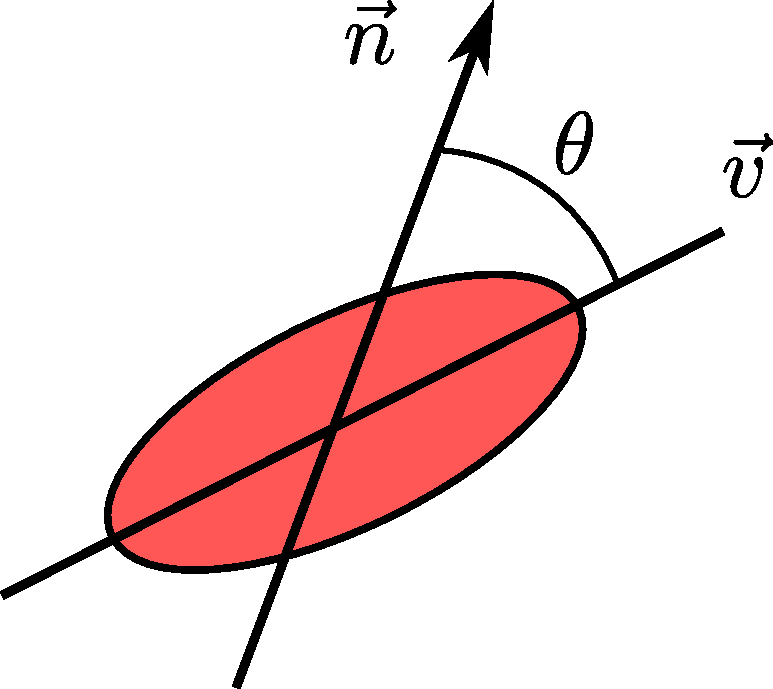
\includegraphics[width=.3\linewidth]{angulo_director}
\caption{Orientación de una molécula de LC con respecto al ángulo
  director en su vecindad.}
\label{fig:angulo_director}
\end{figure}

Un LC con sus moléculas alineadas perfectamente paralelas tiene un
parámetro de orden $S=1$, mientras que un LC con moléculas orientadas
aleatoriamente posee un parámetro $S=0$. El parámetro de orden depende
tanto del tipo de molécula como de la temperatura; en la medida en la
que aumenta la temperatura las moléculas pierden su alineación y el LC
se convierte en un líquido isotrópico. El parámetro de orden gana
importancia cuando se necesita seleccionar un LC que deba ser usado en
rangos de temperatura especiales y se necesite garantizar anisotropía.

\begin{figure}[h!]
\centering
\begin{subfigure}{.4\textwidth}
  \centering
  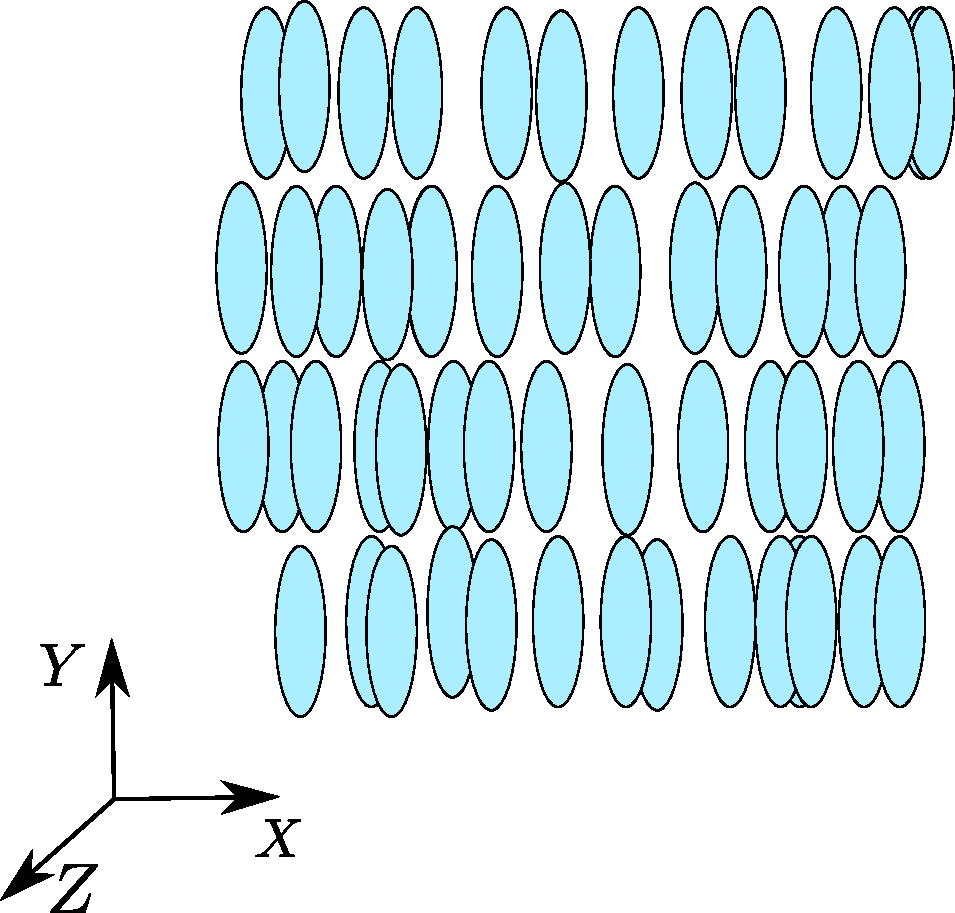
\includegraphics[width=.6\linewidth]{Smetic_LC}
  \caption{Cristal líquido smético.}
  \label{fig:smetic}
\end{subfigure}\qquad
\begin{subfigure}{.4\textwidth}
  \centering
  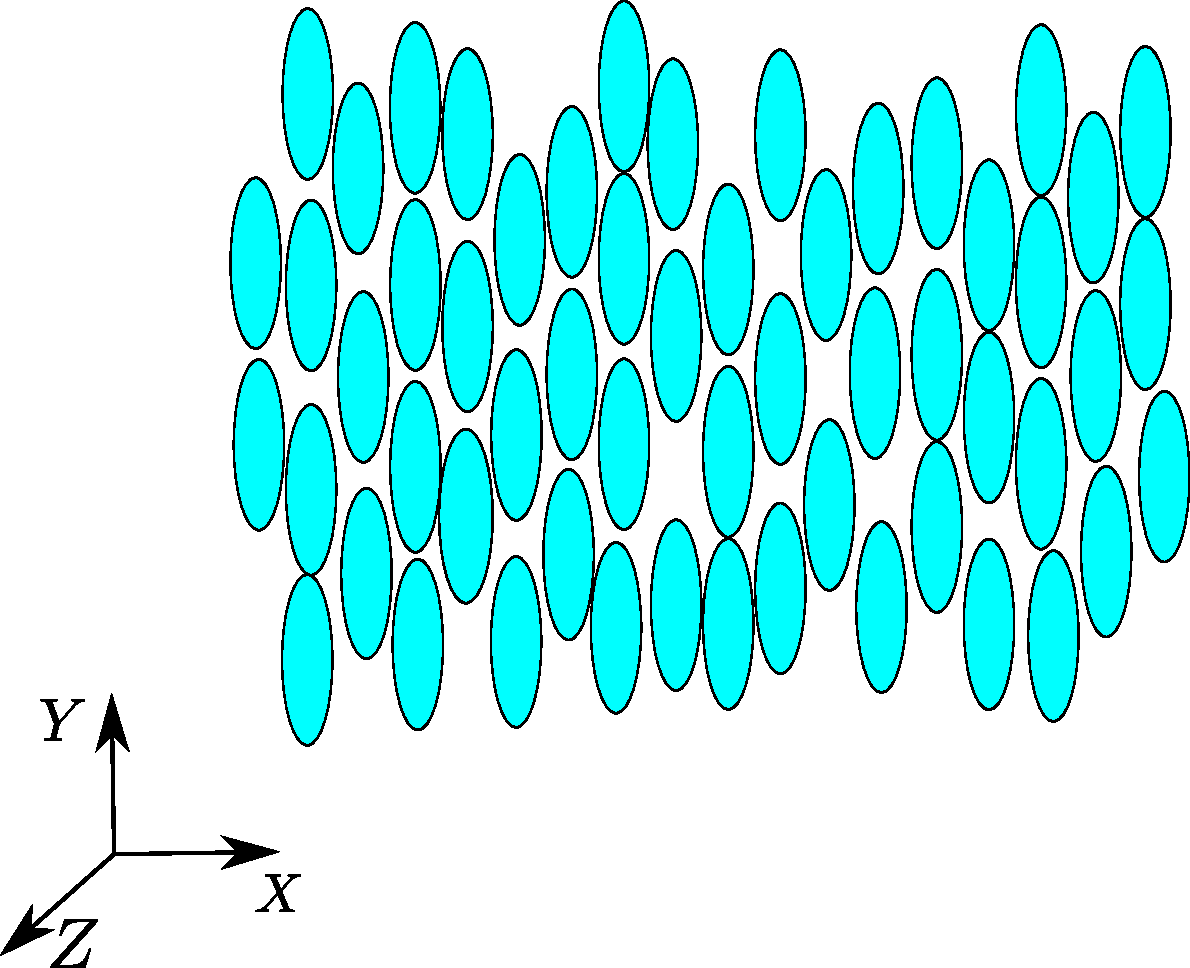
\includegraphics[width=.6\linewidth]{Nematic_LC}
  \caption{Cristal líquido nemático.}
  \label{fig:nematic}
\end{subfigure}\\
\begin{subfigure}{.5\textwidth}
  \centering
  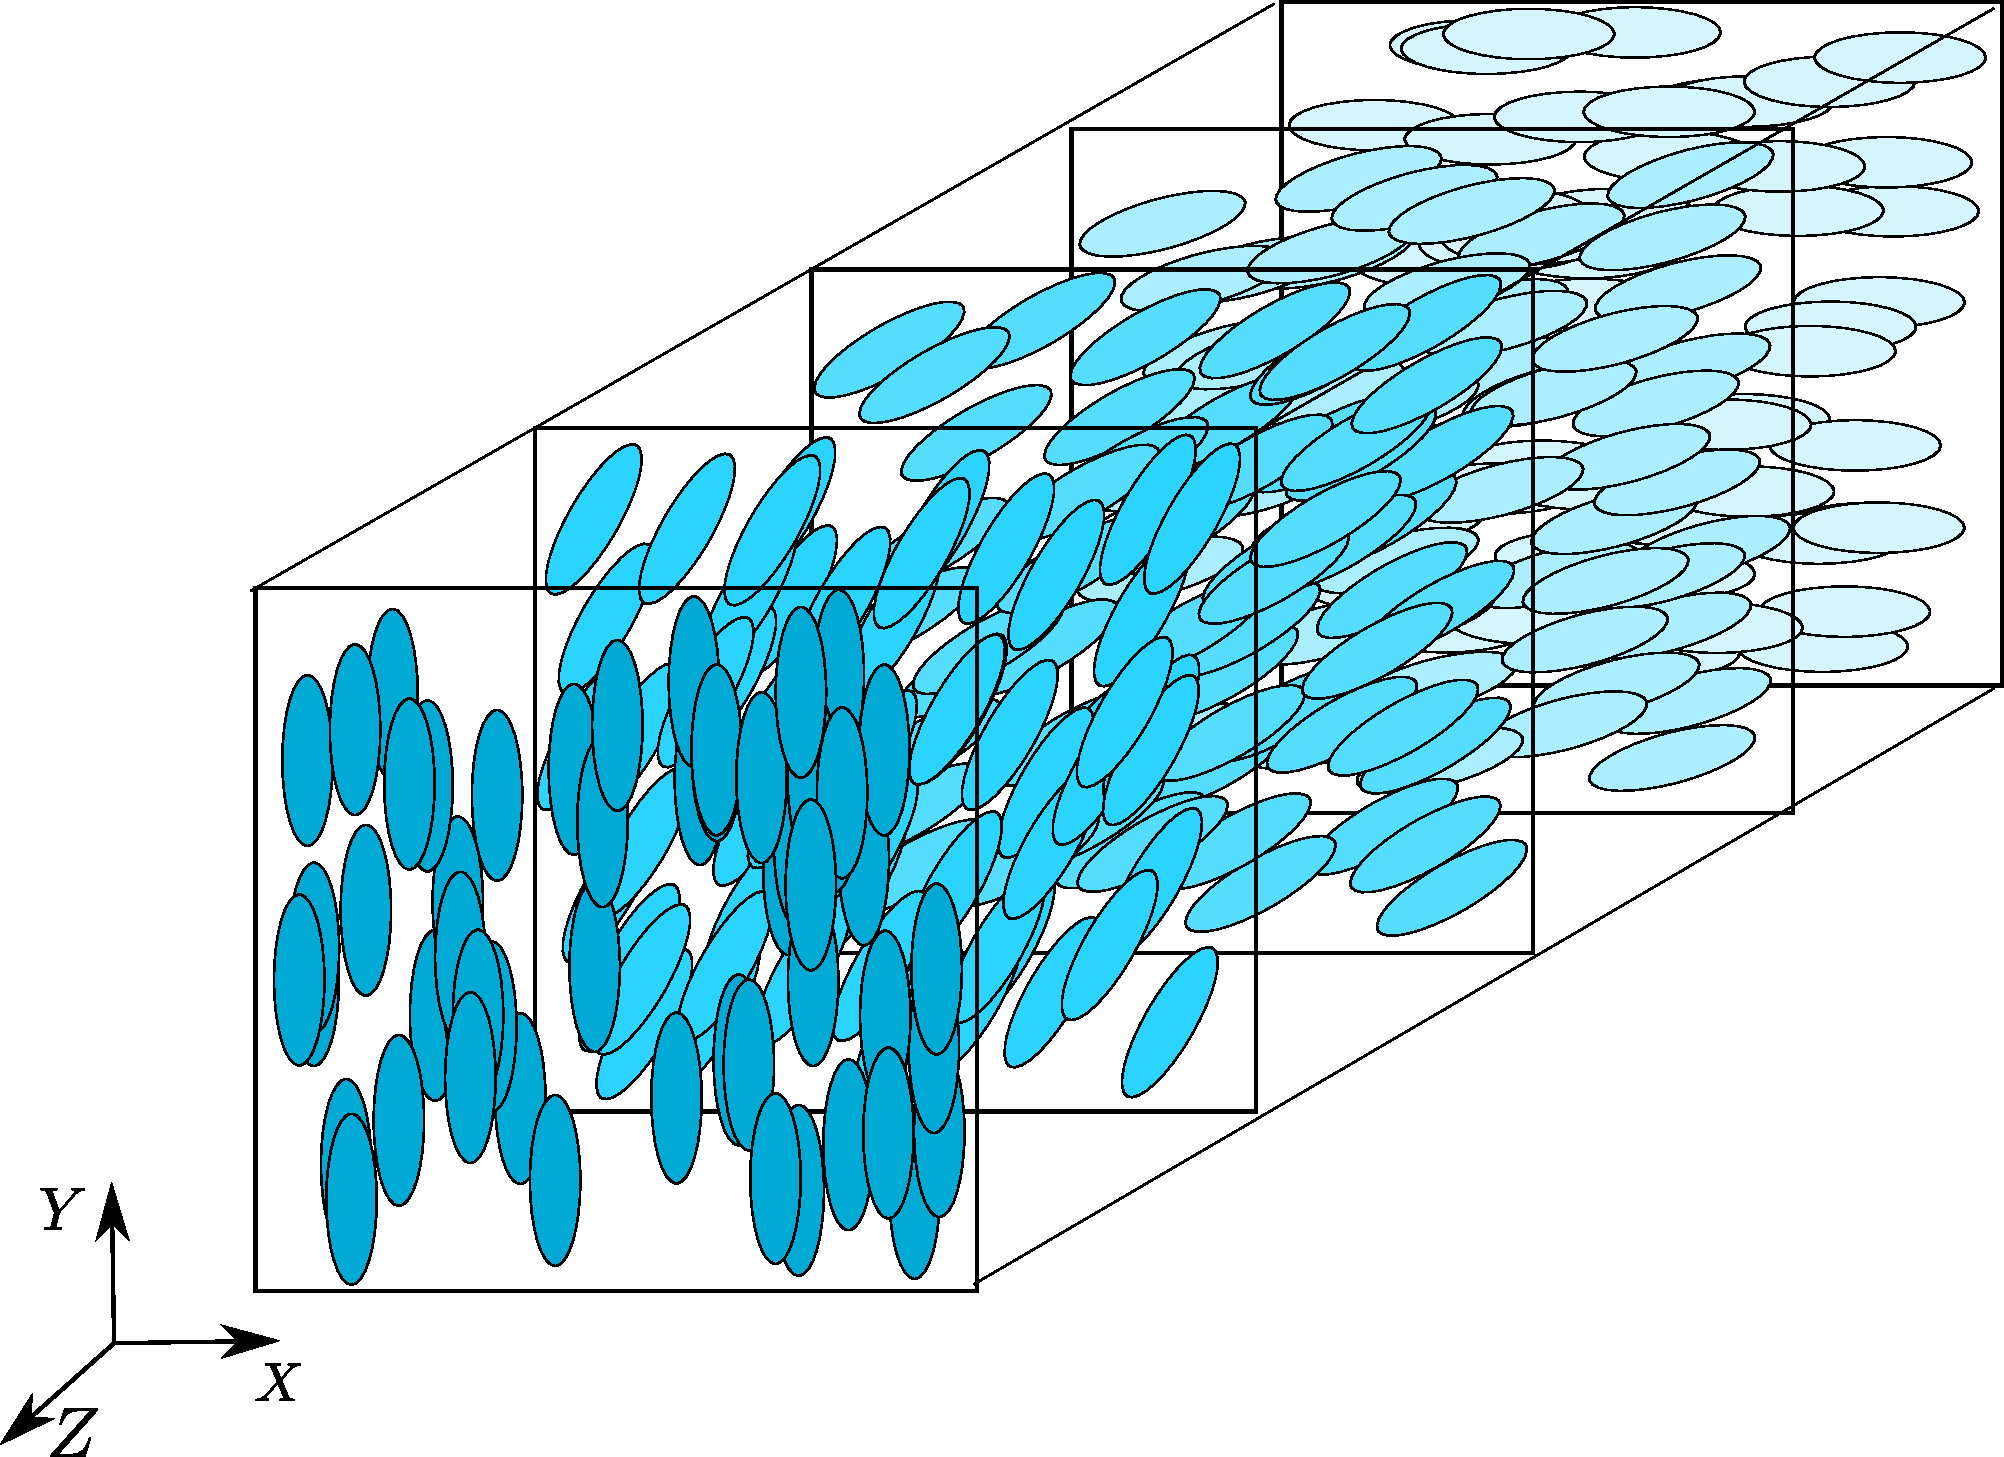
\includegraphics[width=.6\linewidth]{Cholesteric_LC_2}
  \caption{Cristal líquido colestérico.}
  \label{fig:cholesteric}
\end{subfigure}
\caption{Clasificación de los cristales líquidos según su orden.}
\label{fig:CL_clasificacion}
\end{figure}

Los Cristales smeticos como el que se ilustra en la Fig.~
\ref{fig:smetic} se diferencian de los nemáticos en que poseen orden
posicional en una dirección además de orden orientacional. Sin embargo,
este orden viene acompañado de propiedades mecánicas que son menos
convenientes para la construcción de LCDs y por ello las fases
nemáticas y colestéricas son las que tienen mayor número de
aplicaciones en dispositivos electro ópticos. 
A diferencia de las fases smetica y nemática que tienen un solo vector
de orientación, en los cristales líquidos colestéricos el vector
director varía a través del medio de una forma bien
definida y por ello se consideran medios inhomogeneos. Generalmente la
variación es helicoidal como la que se ve en la Fig.~\ref{fig:cholesteric}.   
La variable que caracteriza un cristal líquido colestérico es el
ángulo de inclinación o pitch que forman las moléculas inclinadas con
respecto al eje óptico del material. 


\subsubsection{Las pantallas de cristal líquido nematico retorcido.}


Los moduladores de LC de transmisión que se usan para proyección se
construyen usando una configuración conocida como \textbf{Twisted
Nematic} (\acrshort{TN-LCD}) o nemáticos retorcidos. Los TN-LCD son
dispositivos como el que se ilustra en la Fig.~\ref{fig:tn-lcd} en
los cuales una  solución de cristal líquido nemático se inyecta entre
dos superficies rígidas transparentes que han sido rayadas o frotadas
a lo largo de una dirección preestablecida. Este proceso se conoce
rayado direccional. Las moléculas del LC en
contacto con las superficies transparentes se adhieren a los canales
microscópicos que resultan del rayado, tomando así una
dirección preferencial en ese plano. Cuando las 
direcciones de rayado de las superficies en ambos extremos no
coinciden, la dirección preferente de orientación de las moléculas
cambia gradualmente en profundidad desde la dirección del plano de
entrada hasta la del plano de salida como se ve en la Fig.~
\ref{fig:tn-lc}.  El resultado es un cristal líquido inhomogeneo
parecido a un cristal colestérico en el cual la orientación de las
moléculas varía de forma lineal.

\begin{figure}[h!]
\centering
\begin{subfigure}{.45\textwidth}
  \centering
  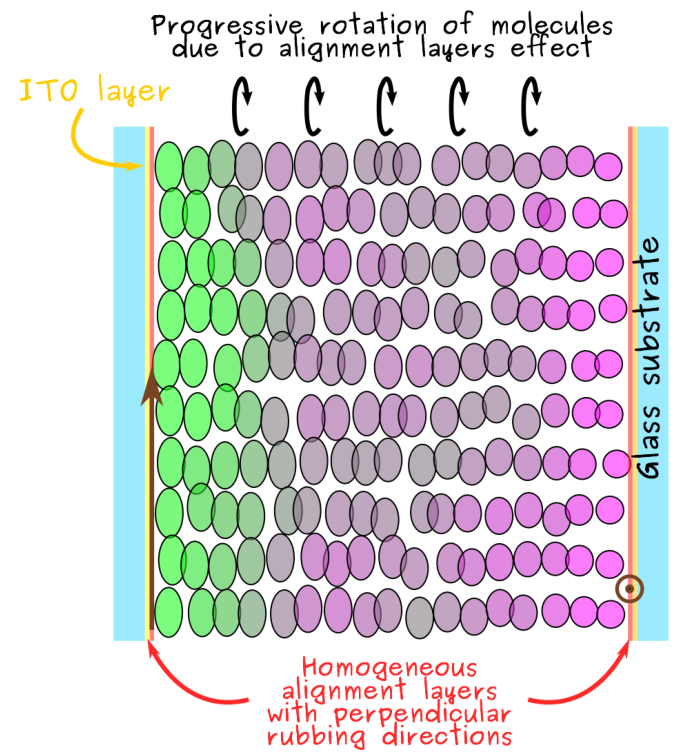
\includegraphics[width=.8\linewidth]{tn-lcd}
  \caption{Esquema de un TN-LCD cuando no hay un voltaje entre las placas.}
  \label{fig:tn-lc}
\end{subfigure}\qquad
\begin{subfigure}{.45\textwidth}
  \centering
  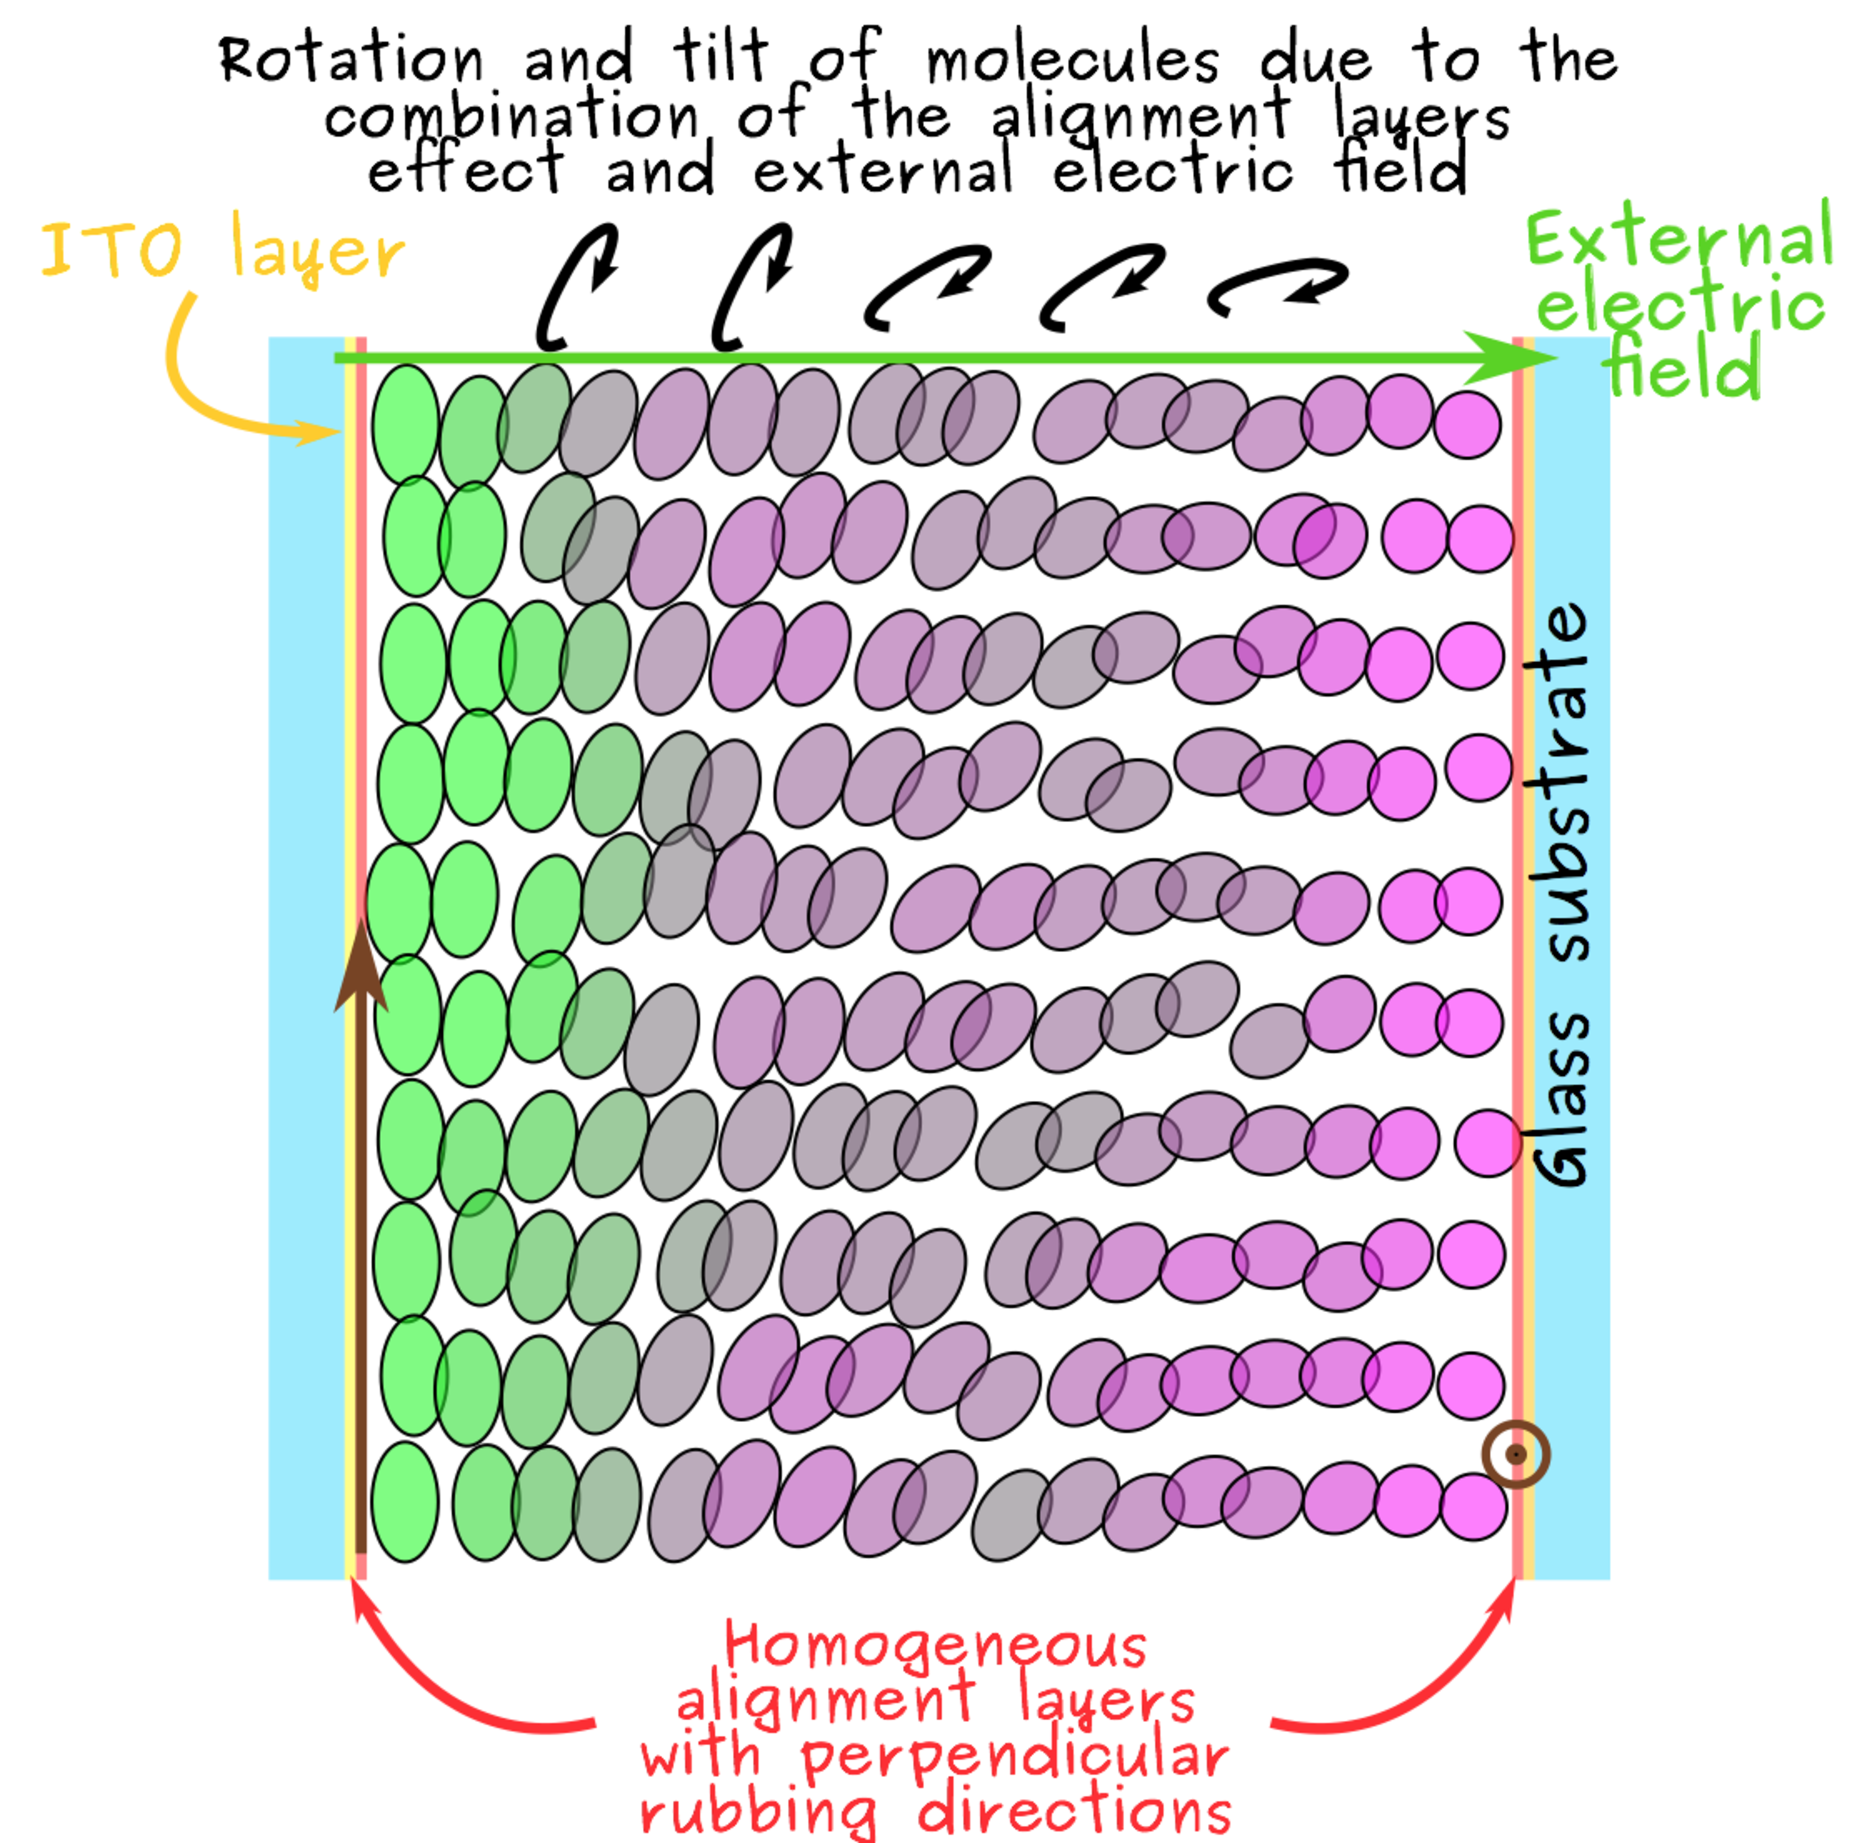
\includegraphics[width=.8\linewidth]{tn-lcd-voltage}
  \caption{Esquema de un TN-LCD dónde se aplica una diferencia de
    potencial entre placas}
  \label{fig:tn-lc-voltage}
\end{subfigure}
\caption[Arquitectura de un TN-LCD]{Arquitectura de un TN-LCD cuando (a) está apagado, y (b) se
  le aplica una diferencia de potencial. Tomado de Nestor Uribe \citepChGen{UribePatarroyo2011}}
  \label{fig:tn-lcd}
\end{figure} 

Generalmente las direcciones de frotado en las superficies de entrada
y salida son ortogonales de tal forma que las moléculas a la salida experimentan
una rotación de 90 grados con respecto a las de la entrada. Ante la
presencia de un campo eléctrico a lo largo del cristal las moléculas
experimentan una inclinación que es proporcional a la diferencia de
potencial entre las placas tal y como se ilustra en la Fig.~
\ref{fig:tn-lc-voltage}. Al ser moléculas alargadas y polares
experimentan un torque que atrae a la parte negativa de la molécula
hacia el electrodo positivo del  dispositivo y viceversa. La
inclinación es proporcional al voltaje aplicado y es de mayor magnitud
en las regiones más alejadas de las paredes del dispositivo. La
configuración TN ha sido seleccionada para muchos
dispositivos electro ópticos comerciales porque afecta 
la polarización de la luz que incide sobre ella. El objetivo de los
autores que han caracterizado moduladores de transmisión ha sido
principalmente el de describir matemáticamente y de forma robusta las
propiedades ópticas de dispositivos que tienen cristales líquidos de
esta naturaleza.  

En lo que sigue se presentarán las herramientas que son
base para la descripción matemática de campos ópticos polarizados, y
se aplicará para la construcción de un modelo de TN-LCD.

\subsection{Polarización de la luz}

En la teoría electromagnética de la luz se representan los campos
ópticos como ondas que se propagan en el espacio vacío. Un haz de luz
se puede representar tanto por su vector de campo eléctrico como
magnético y ambos son perturbaciones de carácter periódico. Si el
medio de propagación es isotrópico, la dirección de la perturbación 
es transversal, es decir ortogonal a la dirección de propagación
($\mathbf{k}\cdot\mathbf{E}$). Para haces planos monocromáticos se
suele usar la siguiente expresión para el campo eléctrico:  

\begin{align}
\mathbf{E} &=\Re\left[\mathbf{A}e^{i\left( \omega t -\mathbf{k}\cdot \mathbf{r}\right)}\right]\label{eq:complex_field},\\
\mathbf{E} &=\mathbf{A}\cos{ \left(\omega t -\mathbf{k}\cdot
    \mathbf{r}\right)},\notag
\end{align}
dónde, $i = \sqrt{-1}$, $\omega$ es la frecuencia temporal, $\mathbf{k}$ es el vector de
onda o frecuencia espacial, y $\mathbf{A}$ determina la amplitud.
Las frecuencias espacial y temporal se relacionan por medio de la
longitud de onda  ($\lambda$) y el índice de refracción del medio ($\mathbf{n}$) con la
siguiente expresión:

$$\mathbf{k} = \mathbf{n} \frac{2\pi}{\lambda}.$$

Dado que son ortogonales, las variaciones del campo se pueden
representar sobre un plano que es 
ortogonal a la dirección de propagación ($z$ en nuestro caso), y ese plano se puede
representar a su vez por dos vectores que son ortogonales entre si
($x$, $y$).
Cuando la variación del campo sucede sobre una dirección preferencial
se dice que la luz es polarizada, y esa dirección se puede descomponer
como una combinación lineal de las variaciones mutuamente independientes
sobre cada uno de los ejes que forman el plano:

\begin{align}
\mathbf{E} &= E_x +E_y, \notag\\
E_x &= A_x\cos{ \left(\omega t -kz+\delta_x\right)} \label{eq:xcomp},\\
E_y &= A_y\cos{ \left(\omega t -kz+\delta_y\right)}\label{eq:ycomp}.
\end{align}

Se ha separado entonces el campo en sus componentes vertical ($y$) y
horizontal ($x$), cada una con su respectiva amplitud ($A_x,A_y$) y
retardo en fase ($\delta_x,\delta_y$). Dado que las amplitudes son
positivas las fases se dan en el rango $-\pi<\delta_{x,y}<\pi$.
La representación en componentes perpendiculares se asemeja a un
sistema acoplado de osciladores armónicos que oscilan a una misma
frecuencia. Si se dibuja la suma vectorial de las componentes $x$, y $y$ como
un vector que va desde el origen hasta el punto ($E_x,E_y$) y luego se
avanza en el tiempo, la trayectoria que describe la punta del vector
será una curva elíptica como la que 
se muestra en la Fig.~\ref{fig:ellipse_clean} . Si en cambio se congela el tiempo y se gráfica
el desplazamiento de la punta del vector en el espacio se obtiene una curva
helicoidal como en la Fig.~\ref{fig:trayectory_clean}. En estos dibujos se ha
escogido representar una elipse por que es el caso más general de polarización. Sin
embargo, la relación entre las amplitudes ($A_y/A_x$) y la
diferencia de fases ($\delta = \delta_y-\delta_x$) entre las componentes del
campo determina si la polarización es lineal ($\delta = 0$), circular
($\delta =\pm \frac{\pi}{2}, A_y/A_x=1$) o elíptica, y la orientación del eje
mayor de la elipse con respecto al eje $x$.

\begin{figure}[h!]
\centering
\begin{subfigure}{.45\textwidth}
  \centering
  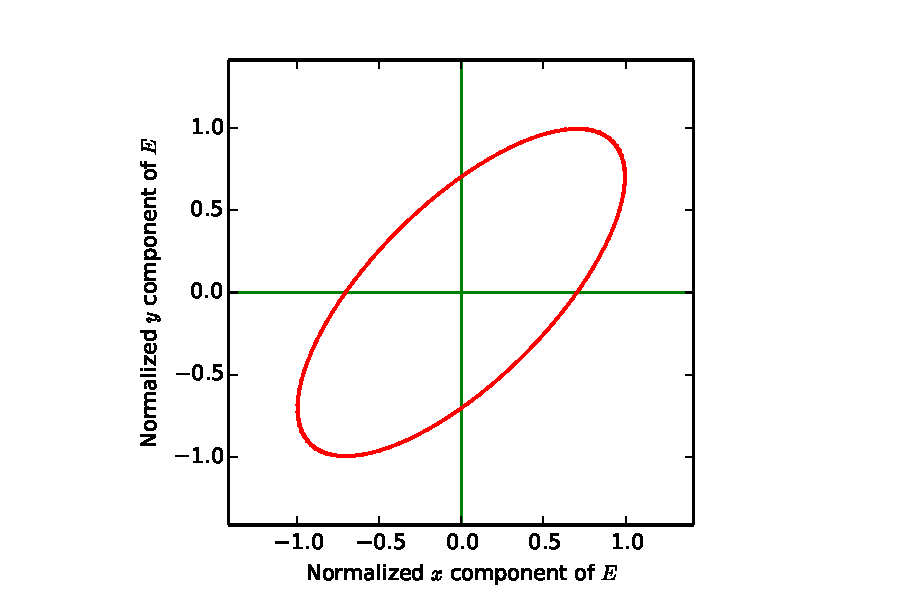
\includegraphics[width=1\linewidth]{ellipse_clean}
  %\caption{Elipse arbitraria que resulta cuando se observa la
   % variación temporal de un campo sobre el plano.}
  \caption{}
\label{fig:ellipse_clean}
\end{subfigure}\qquad
\begin{subfigure}{.45\textwidth}
  \centering
  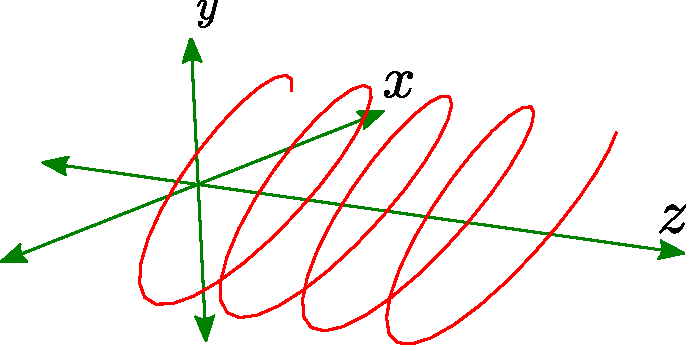
\includegraphics[width=.8\linewidth]{trayectory_clean}
 % \caption{Trayectoria helicodidal de la variación espacial de un
  %  campo óptico a lo largo de $z$.}
  \caption{}
  \label{fig:trayectory_clean}
\end{subfigure}
\caption[Distintas representaciones del campo eléctrico para ilustrar
la polarización]{Representaciones de la posición de un vector de campo
  eléctrico con polarización elíptica cuando (a) se analiza en un
  punto en el espacio, y (b) se  congela el tiempo.} 
\label{fig:general_field}
\end{figure} 

Desde el punto de vista matemático, la Fig.~\ref{fig:ellipse_clean} se describe por medio de la Eq.~\ref{eq:ellipse} que es la ecuación de una cónica y se puede obtener
a partir de las expresiones (\ref{eq:xcomp}) y (\ref{eq:ycomp}). 

Si $\delta = \delta_y-\delta_x$ y $z=0$,
entonces el campo se puede escribir como

\begin{align*}
E_x &= A_x\cos{ \left(\omega t \right)},\\
E_y &= A_y\cos{ \left(\omega t -\delta\right)}.
\end{align*}
Y se puede despejar los términos correspondientes al $\sin$ y $\cos$
 \begin{align*}
\cos{\omega t} &=\frac{E_x}{A_x},\\
\sin^2{\omega t} &= 1-\left(\frac{E_x}{A_x}\right)^2,\\
\sin{\omega t} &= \sqrt{1-\left(\frac{E_x}{A_x}\right)^2}.
\end{align*}
Por otra parte se tiene
\begin{equation}
  \label{eq:Ey-2}
E_y = A_y\left( \cos{\omega t}\cos{\delta}+\sin{\omega
    t}\sin{\delta}\right).  
\end{equation}
Reemplazando $\sin{\omega t} $ y $\cos{\omega t} $ en la expresión
(\ref{eq:Ey-2}) obtenemos
\begin{align}
E_y &= \frac{A_yE_x}{A_x}\cos{\delta} +
A_y\sqrt{1-\frac{E_x}{A_x}}\sin{\delta},\notag\\
\frac{E_y}{A_y} - \frac{E_x}{A_x}\cos{\delta}  &= 
\sqrt{1-\left(\frac{E_x}{A_x}\right)^2}\sin{\delta}.\label{eq:ellipse_nos}
\end{align}
Elevando al cuadrado la Eq.~(\ref{eq:ellipse_nos}) y organizando
términos, obtenemos la ecuación general de una elipse inscrita en un
rectángulo con lados $2A_x$, $2A_y$ 
\begin{equation}
\left(\frac{E_x}{A_x}\right)^2+\left(\frac{E_y}{A_y}\right)^2-2\frac{\cos{\delta}}{A_xA_y}E_xE_y
= \sin^2{\delta}.
\label{eq:ellipse}
\end{equation}
Se puede ahora plantear una rotación de un ángulo $\phi$ con respecto
al eje horizontal ($x$) sobre el sistema de coordenadas  como se
muestra en la Fig.~\ref{fig:ellipse} para que
el eje mayor de la elipse quede alineado con el eje
\textit{horizontal} del nuevo sistema. 
\begin{figure}[h!]
\centering
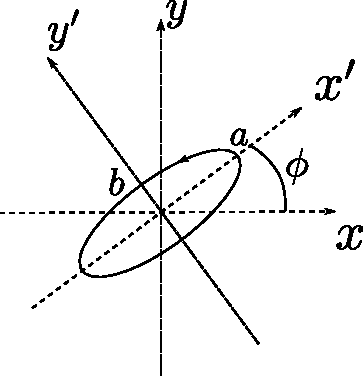
\includegraphics[scale = 1]{ellipse}
\caption[Rotación del sistema de coordenadas de la elipse de polarización]{Rotación del sistema de coordenadas un ángulo $\phi$.}
\label{fig:ellipse}
\end{figure}
Haciendo esto, se lleva la
Eq.~(\ref{eq:ellipse}) a la forma más conocida de la Eq.~(\ref{eq:new_ellipse})
\begin{equation}
\left(\frac{E_{x'}}{a}\right)^2+\left(\frac{E_{y'}}{b}\right)^2 = 1,
\label{eq:new_ellipse}
\end{equation}
dónde $a$ y $b$ son los semi ejes mayor y menor, y $E_{x'}$, $E_{y'}$
son las componentes del campo eléctrico en las direcciones $x'$,
$y'$. Los semiejes de la elipse están dados por las siguientes
expresiones \citepChGen{Yariv2002}:
\begin{align*}
a^2 = A_x\cos^2{\phi}+A_y^2\sin^2{\phi} +2A_xA_y \cos{\delta}\cos{\phi}\sin{\phi},\\
b^2 = A_x\sin^2{\phi}+A_y^2\cos^2{\phi} -2A_xA_y \cos{\delta}\cos{\phi}\sin{\phi}.
\end{align*}

La elipticidad se define como la razón entre el eje menor y el eje
mayor de la elipse $e=\pm\frac{b}{a}$ de tal forma que si el semi eje
menor es cero, la elipse se vuelve una linea y por tanto se dice que
la polarización es lineal en la dirección de $a$. Si por el contrario
los dos semi ejes tienen  la misma longitud, la ecuación de la elipse
se vuelve la de un círculo, y se dice que la polarización es
circular como en la Fig.~\ref{fig:circular_polarizations}(a). 
El signo de la elipticidad determina el sentido 
de giro de la hélice, si el signo es positivo la elipse es circular
izquierda como en la Fig.~\ref{fig:circular_polarizations}(b) y es
circular derecha 
cuando el signo es negativo (Fig.~\ref{fig:circular_polarizations}(c)). Cabe
anotar que el sentido de giro de la polarización es una convención
que varía según el autor, algunos autores como \citetChGen{Yariv2002} interpretan el sentido de giro como
si se congelara el tiempo y se siguiera la punta del vector
$\mathbf{E}$ desde el momento inicial en adelante. Sin embargo, otros
autores como \citetChGen{Hecht2001}
interpretan el sentido de giro como si en un punto fijo vieran girar
el vector $\mathbf{E}$ que les llega en la medida que pasa el tiempo. 
En este documento hemos decidido escoger la primera convención dado
que es la predominante en las referencias que tratan el análisis de
cristales líquidos como elementos que afectan la polarización. 
\begin{figure}[h!]
\centering
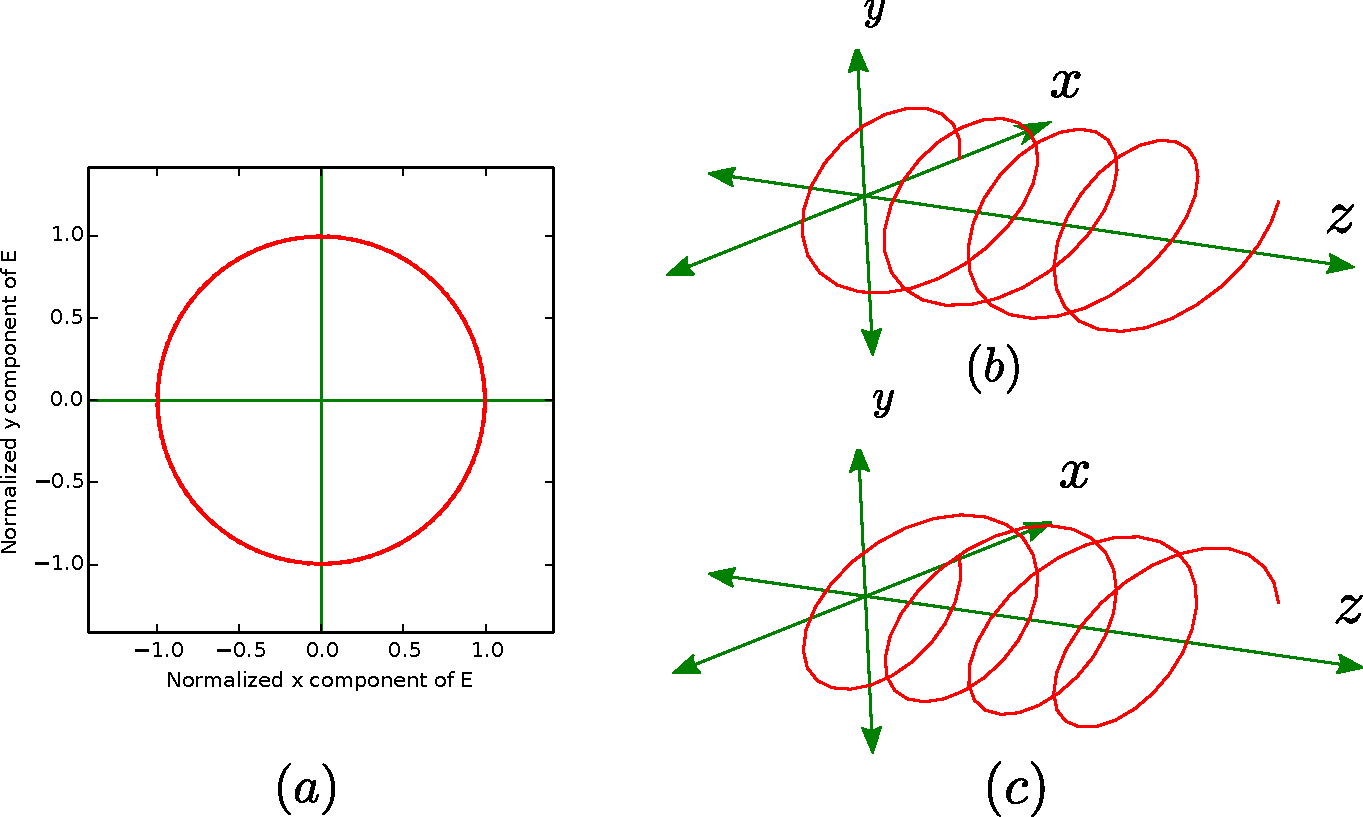
\includegraphics[scale=.5]{circular_polarizations}
\caption[Estados de polarización circular]{(a) Esquema de un estado de polarización circular en donde los semiejes
  de la elipse son iguales. La polarización circular izquierda (b) se da
cuando $e=\frac{b}{a}$ y la derecha (c) cuando  $e=-\frac{b}{a}$.}
\label{fig:circular_polarizations}
\end{figure}

Una ellipse de polarización arbitraria se puede expresar entonces
conociendo su elipticidad ($e$) y su ángulo de inclinación ($\phi$)
con respecto al eje horizontal. Estas dos características se pueden
parametrizar como dos ángulos que se dan en
términos de las amplitudes máximas del campo $A_x$, $A_y$
y el retardo entre componentes $\delta$. Por una parte, el ángulo de
inclinación se encuentra interpretando la Eq.~(\ref{eq:ellipse}) en
su forma bilineal de la forma
\begin{equation}
\begin{pmatrix}
E_x & E_y
\end{pmatrix}
\begin{pmatrix}
\frac{1}{A_x^2} & -\frac{\cos{\delta}}{A_xA_y}\\
 -\frac{\cos{\delta}}{A_xA_y} & \frac{1}{A_y^2} 
\end{pmatrix}
\begin{pmatrix}
E_x \\ E_y
\end{pmatrix}
=\sin^2{\delta},
\end{equation}
sacando factor común $\frac{1}{A_x^2} $ se obtiene
\begin{equation}
\begin{pmatrix}
E_x & E_y
\end{pmatrix}
\begin{pmatrix}
1 & -\frac{A_x\cos{\delta}}{A_y}\\
 -\frac{A_x\cos{\delta}}{A_y} & \frac{A_x/2}{A_y^2} 
\end{pmatrix}
\begin{pmatrix}
E_x \\ E_y
\end{pmatrix}
=A_x/2\sin^2{\delta},
\end{equation}
o en forma compacta
\begin{equation}
\begin{pmatrix}
E_x & E_y
\end{pmatrix}
\begin{pmatrix}
1 & a\\
 a & b 
\end{pmatrix}
\begin{pmatrix}
E_x \\ E_y
\end{pmatrix}
=c.
\end{equation}
%http://mpalffy.lci.kent.edu/Optics/Chapters/Ch7_Polarized%20Light.pdf

Una \href{http://es.wikipedia.org/wiki/Cu\%C3\%A1drica}{\textbf{cuádrica o superficie cuádrica}} es una  hipersuperficie D-dimensional
representada por una ecuación de segundo grado con 
coordenadas espaciales. Si estas coordenadas son $\{x_1,
x_2, ... x_D\}$, entonces la cuádrica típica en ese espacio se define
mediante la ecuación algebraica: 
\[ \sum_{i,j=1}^D Q_{i,j} x_i x_j + \sum_{i=1}^D P_i x_i + R = 0. \]
El caso particular en el cual solo hay dos dimensiones y los valores
$P_i$ son todos 0, es el de una elipse. En nuestro caso, tenemos en
notación matricial:
\[ \mathbf{E}^TQ\mathbf{E} + R= 0, \]
con
\[
Q=
\begin{pmatrix}
1 & a\\
 a & b 
\end{pmatrix}.
 \]
y $R=-c = -A_x/2\sin^2{\delta}$. Ahora, los autovalores de una elipse
representada por su forma matricial están asociados con la
dirección de sus ejes principales, y apuntan en la dirección de los
puntos máximos \citepChGen{Palffy1998}. Como nuestra incógnita es el ángulo
que determina la dirección de los puntos máximos, podemos escribir la
siguiente ecuación de autovalores para despejar $\phi$\footnote{
\url{http://en.wikipedia.org/wiki/Quadratic_form}}
\[\begin{pmatrix}
1 & a\\
 a & b 
\end{pmatrix} 
\begin{pmatrix}
\cos{\phi}\\
 \sin{\phi} 
\end{pmatrix} =
\lambda \begin{pmatrix}
\cos{\phi}\\
 \sin{\phi} 
\end{pmatrix} ,
\]
desarrollando, se obtienen las siguientes dos ecuaciones:
\begin{align*}
\cos{\phi} +a\sin{\phi} &= \lambda\cos{\phi},\\
a\cos{\phi} +b\sin{\phi} &= \lambda\sin{\phi}.
\end{align*}
Despejando $\lambda$ e igualando las ecuaciones se llega a una
expresión dependiente de un ángulo doble:
\[1+a\tan{\phi} = \frac{a}{\tan{\phi}}+b,\]
\[b-1= a\tan{\phi} -\frac{a}{\tan{\phi}},\]
\[ b-1=a\left(\frac{\tan^2{\phi} -1}{\tan{\phi}}\right),\]
\[\tan{2\phi} =\frac{2a}{b-1}.\]
Finalmente, reemplazando $a$, y $b$ se tiene el ángulo de inclinación
de la elipse:
\begin{equation*}
\phi = \frac{1}{2}\tan^{-1}{\left(\frac{2A_xA_y}{A_x^2-A_y^2}\cos{\delta}\right)}.
\end{equation*}
Siguiendo un esquema similar, aunque más tedioso se encuentra el
ángulo de elipticidad ($\theta = \tan^{-1}{e}$) en términos de la
función seno como:
\begin{equation*}
\theta = \frac{1}{2}\sin^{-1}{\left(\frac{2A_xA_y}{A_x^2+A_y^2}\sin{\delta}\right)}.
\end{equation*}
A la hora de despejar $\phi$ y $\theta$ reemplazando valores en la
primera ecuación usando un computador se aconseja reemplazar la función
$\tan^{-1}$ por la función atan2, que es popular en paquetes de
cálculos numéricos (como numpy) o lenguajes de programación como
Matlab, porque permite evitar las singularidades que ocurren cuando el argumento de la
función tangente inversa es $\pi/2$.

\subsection{El formalismo de Jones}

Se conoce como formalismo de Jones al uso de una representación
vectorial para describir campos ópticos coherentes y monocromáticos cuando es
importante la naturaleza vectorial de la luz y la polarización.  
En el esquema de Jones los campos ópticos con dos componentes ortogonales se
representan como un vector con elementos complejos conocido como
vector de Jones. Las dos componentes complejas del campo en la Eq.~(\ref{eq:complex_field}) se representan como elementos de un vector
columna conocido como vector de Jones:
 
\begin{equation}
\mathbf{J} =\begin{pmatrix} A_xe^{i\delta_x}\\A_ye^{i\delta_y}\end{pmatrix}.
\label{eq:jones_vector}
\end{equation}
Siendo un vector complejo, $\mathbf{J}$ no es una cantidad observable
en el espacio físico. Para obtener por ejemplo, la
componentente  $x$ del campo eléctrico se hace la operación $E_x(t) = \Re
\left[J_xe^{i\omega t}\right]$.
Para el estudio de la polarización conviene representar el vector de
Jones en su forma normalizada, es decir tal que cumpla la
condición, $$\mathbf{J}^{\dagger}\mathbf{J}=1,$$
dónde el símbolo $\dagger$ representa la transpuesta conjugada.
La normalización se logra parametrizando las amplitudes con el ángulo
del vector que forman, $$\tan{\psi}=\frac{\sin{\psi}}{\cos{\psi}}=\frac{A_y}{A_x},$$
de esta forma $A_y=\sin{\psi}$ y $A_x = \cos{\psi}$. Adicionalmente,
la fase de las componentes se acostumbra a escribir en su forma
relativa y con respecto a la componente $y$ como se muestra en la
expresión (\ref{eq:normalized_jones_vector}).

\begin{equation}
\mathbf{J(\psi,\delta)} =\begin{pmatrix} \cos{\psi}\\\sin{\psi}e^{i\delta}\end{pmatrix}.
\label{eq:normalized_jones_vector}
\end{equation}

\subsubsection{Algunos estados de polarización importantes}
Como se dijo antes, las polarizaciones lineales se obtienen cuando las
componentes están en fase, es decir que $\delta =
\delta_y-\delta_x=0$. Sin embargo, la condición también se cumple cuando las
diferencias de fase entre las componentes son múltiplos de $\pi$. 
A continuación se muestran seis estados de polarización conocidos
como los \textbf{estados degenerados de polarización}
\citepChGen{Collett2005} que son importantes tanto en la teoría de
polarización de Jones como en la de Stokes para la composición y
detección de estados de polarización elípticos.
Los primeros dos estados degenerados corresponden a las polarizaciónes
lineales ($\delta = n\pi$ ) horizontal y vertical que se dan cuando $\psi
= n\pi$ y $\psi = \frac{\pi}{2}(2n+1)$ respectivamente:
\begin{align*}
\mathbf{H} &=\begin{pmatrix}1\\0\end{pmatrix},& \mathbf{V} &=\begin{pmatrix}0\\1\end{pmatrix}.
\end{align*}
Luego, están los estados con polarización lineal a $45^{\circ}$ y
$-45^{\circ}$. El primero se da cuando las componentes $x$
y $y$ tienen la misma magnitud y dirección, es decir cuando
$\psi=\frac{\pi}{4}(4n+1)$. La polarización a  $-45^{\circ}$ se da cuando
$\psi=\frac{\pi}{4}(4n-1)$.
\begin{align*}
\mathbf{45^{\circ}}
&=\begin{pmatrix}\cos{\pi/4}\\\sin{\pi/4}\end{pmatrix}=\frac{1}{\sqrt{2}}
\begin{pmatrix}1\\1\end{pmatrix},&
\mathbf{-45^{\circ}} 
&=\begin{pmatrix}\cos{-\pi/4}\\\sin{-\pi/4}\end{pmatrix}=\frac{1}{\sqrt{2}}\begin{pmatrix}1\\-1\end{pmatrix}. 
\end{align*} 
Finalmente, se tienen los estados circulares que consisten en las
polarizaciones circular izquierda y circular derecha. Los estados de
polarozación circulares son tales que
ambas componentes tienen la misma magnitud que los de $\pm45^{\circ}$,
pero el retardo en fase entre ellas es de $\delta = \frac{\pi}{2}$:
\begin{align*}
\mathbf{CD}
&=\begin{pmatrix}\cos{\pi/4}\\\sin{\pi/4}e^{i\frac{\pi}{2}}\end{pmatrix}=\frac{1}{\sqrt{2}}
\begin{pmatrix}1\\i\end{pmatrix},&
\mathbf{CI} 
&=\begin{pmatrix}\cos{-\pi/4}\\\sin{-\pi/4}e^{i\frac{\pi}{2}}\end{pmatrix}=\frac{1}{\sqrt{2}}\begin{pmatrix}1\\-i\end{pmatrix}. 
\end{align*} 
Una característica interesante de los estados lineales y circulares es
que se pueden dar unos como combinación lineal de los otros:
\begin{align*}
\mathbf{CD} &= \frac{1}{\sqrt{2}}\left( \mathbf{H} -
  i\mathbf{V}\right),\\
\mathbf{CI} &= \frac{1}{\sqrt{2}}\left( \mathbf{H} +
  i\mathbf{V}\right),\\
\mathbf{H} &= \frac{1}{\sqrt{2}}\left( \mathbf{CD} +
  \mathbf{CI}\right),\\
\mathbf{V} &= \frac{i}{\sqrt{2}}\left( \mathbf{CD} -
  \mathbf{CI}\right).
\end{align*}
Los vectores de las tres parejas de estados que hemos visto hasta
ahora son bases ortonormales. Esto quiere decir que fuera de estar
normalizados, %son linealmente independientes entre sí, 
si calculamos el producto escalar entre elementos de una misma pareja
obtenemos un valor de 0,
% \begin{equation*}
% \begin{pmatrix}1&0\end{pmatrix}\begin{pmatrix}0\\1\end{pmatrix}=
% \left(\frac{1}{\sqrt{2}}\begin{pmatrix}1&1\end{pmatrix}\right)\left(\frac{1}{\sqrt{2}}\begin{pmatrix}1\\-1\end{pmatrix}\right)  = \left(\frac{1}{\sqrt{2}}
% \begin{pmatrix}1&i\end{pmatrix}\right)\left(\frac{1}{\sqrt{2}}\begin{pmatrix}1\\-i\end{pmatrix}\right)
% = 0.
% \end{equation*}
\begin{equation*}
\mathbf{H^{\dagger}V} = \mathbf{45^{\circ\dagger}-45^{\circ}} =
\mathbf{CD^{\dagger}CI = 0.}   
\end{equation*}
Estos estados se han mencionado porque sirven como base para el espacio
de posibles estados de polarización y serán usados en la sección
\ref{sec:ChGV_med_mod_amp} para producir curvas de modulación de
amplitud que alimentan un modelo de calibración de moduladores capaz
de predecir la modulación para otros estados. 

\subsubsection{Elementos ópticos como operadores en la representación
  de Jones}

Así como en el álgebra lineal se usan matrices para transformar
vectores, en el formalismo de Jones existen operadores que se
representan como matrices 2x2 y que tienen la cualidad de
transformar los campos. Estos operadores se conocen como matrices de
Jones y deben cumplir algunas
propiedades generales \citepChGen{Yariv2002} que se listan a continuación:

\begin{enumerate}
\item La dirección de propagación de un campo determina las
  componentes de la matriz que representa al elemento polarizador. Si
  la incidencia es desde la izquierda $(z=0)$ definimos la matriz $M$ como aquella
  que transforma el vector de entrada en el de salida,
  \begin{equation}
    \begin{pmatrix}
      V_x^{out}\\V_y^{out}
    \end{pmatrix}
    =
    \begin{pmatrix}
      M_{11}&M_{12}\\M_{21} & M_{22}
    \end{pmatrix}
    \begin{pmatrix}
      V_x^{in}\\V_y^{in}
    \end{pmatrix},
    \label{eq:right_propagation}
  \end{equation}
si el vector de entrada ingresa desde la derecha entonces
definiremos una matriz distinta $N$ para representar la transformación:
  \begin{equation*}
    \begin{pmatrix}
      V_x^{out}\\V_y^{out}
    \end{pmatrix}
    =
    \begin{pmatrix}
      N_{11}&N_{12}\\N_{21} & N_{22}
    \end{pmatrix}
    \begin{pmatrix}
      V_x^{in}\\V_y^{in}
    \end{pmatrix}.
  \end{equation*}

Para que se cumpla el principio de simetría temporal, se debe cumplir
que $NM=1$. Si se \textit{rebobina} la propagación en la expresión
(\ref{eq:right_propagation}) el haz de salida 
debería seguir el mismo camino que recorrió a la entrada, y ser
afectado por la matriz $N$ de tal forma que vuelva a la forma que
tenía en un principio,
 \begin{align*}
    \begin{pmatrix}
      V_x^{in}\\V_y^{in}
    \end{pmatrix}
    &=
    \begin{pmatrix}
      N_{11}&N_{12}\\N_{21} & N_{22}
    \end{pmatrix}
    \begin{pmatrix}
      V_x^{out}\\V_y^{out}
    \end{pmatrix},\\
    &=
    \begin{pmatrix}
      N_{11}&N_{12}\\N_{21} & N_{22}
    \end{pmatrix}
    \begin{pmatrix}
      M_{11}&M_{12}\\M_{21} & M_{22}
    \end{pmatrix}
    \begin{pmatrix}
      V_x^{in}\\V_y^{in}
    \end{pmatrix}.\\
  \end{align*}
  Conociendo que las matrices están asociadas a un mismo elemento se
  debe cumplir que $N$ sea la transpuesta de $M$
  \begin{align*}
    N_{11}&=M_{11},&    N_{12}&=M_{21},&     N_{21}&=M_{12}, &     N_{22}&=M_{22}.
  \end{align*}
Esta relación es importante para analizar sistemas en los cuales la
luz debe pasar dos veces por el LC en sentidos opuestos, caso especial
es el de los SLM's de reflexión en los cuales hay una
superficie especular de un lado.

\item Tanto la matriz $M$ como la $N$ son operadores unitarios,
  \begin{align*}
    M^{\dagger} M &= 1,& N^{\dagger}N &=1.
  \end{align*}
Dónde el símbolo $\dagger$ indica que se saca el conjugado hermítico
de $M$,
\begin{equation*}
M^{-1}=M^{\dagger}=
  \begin{pmatrix}
      M_{11}^*&M_{21}^*\\M_{12}^* & M_{22}^*
    \end{pmatrix}.
\end{equation*}
\item Las matrices de Jones son también unimodulares es decir
\begin{equation}det(M) = det(M^{\dagger})  = M_{11}M_{22}-M_{12}M_{21} = 1.\label{eq:unimodular}\end{equation} 
Si asumimos que $M^{-1}$ es
\begin{equation*}
  M^{-1}=
  \begin{pmatrix}
    M_{22}&-M_{12}\\-M_{21}&M_{11}
  \end{pmatrix},
\end{equation*}
se ve que cumple con la relación $M^{-1}M = 1$:
\begin{align*}
    \begin{pmatrix}
    M_{22}&-M_{12}\\-M_{21}&M_{11}
  \end{pmatrix}
\begin{pmatrix}
      M_{11}&M_{12}\\M_{21} & M_{22}
    \end{pmatrix}
&=
    \begin{pmatrix}
 M_{22}M_{11}-M_{12}M_{21}     & M_{22}M_{12}-M_{12}M_{22}\\
-M_{11}M_{21}+M_{11}M_{21}    & -M_{12}M_{21} + M_{11}M_{22} 
    \end{pmatrix},\\
&=
\begin{pmatrix}
  1 &0\\0&1
\end{pmatrix}.
\end{align*}
Con esto, se puede simplificar la forma de una matriz de Jones a
partir de las siguientes relaciones,
\begin{align*}
  M_{21} &= - M_{12}^*, & M_{22} = M_{11}^*,
\end{align*}
obteniendo una forma de la matriz que depende de sólo dos números
complejos:
\begin{align}
  M&=
  \begin{pmatrix}
    A & B \\-B^* & A^*
  \end{pmatrix}\\
&=
  \begin{pmatrix}
    X+iY & Z+iW \\-Z+iW& X-iY
  \end{pmatrix}
\label{eq:general_jones_matrix}
\end{align}

Tener la matriz en esta forma facilita encontrar los parámetros de elementos
ópticos desconocidos como un SLM porque reduce el número de incógnitas.

\end{enumerate}

Los operadores que se verán a
continuación hacen referencia a dos tipos de elementos ópticos que se
utilizan en el laboratorio para modificar los estados de polarización
de una onda, estos son, polarizadores y retardadores. Los polarizadores
son elementos que afectan únicamente la amplitud y los
retardadores introducen retardos de la fase entre las componentes del campo.
Por una parte, los polarizadores horizontales son elementos que sólo
dejan pasar la componente $x$ del campo, y se representan con la
matriz de la Eq.~(\ref{eq:Px_matrix}),
\begin{equation}
P_x = \begin{pmatrix}1 &0\\0&0\end{pmatrix}.
\label{eq:Px_matrix}
\end{equation}
Si llega cualquier campo al polarizador horizontal este dejará pasar
sólo la componente $x$ tal y
como se muestra en la Fig.~\ref{fig:linear_polarizer}. 
\begin{figure}[h!]
\centering
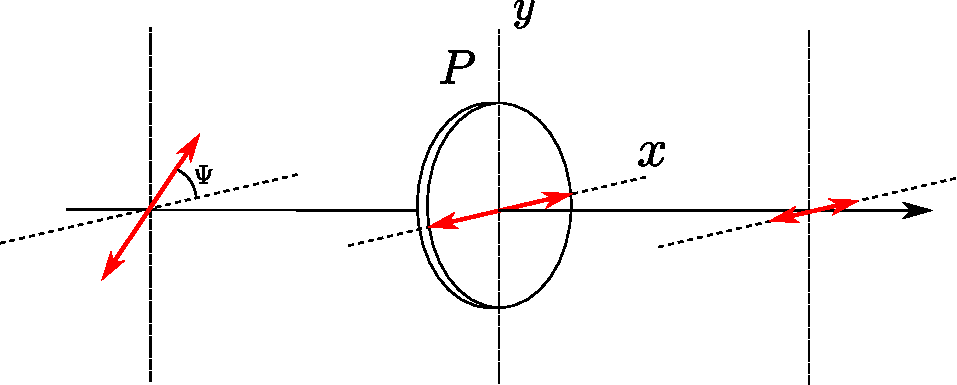
\includegraphics[scale = .7]{linear_polarizer}
\caption{Propagación de un estado de polarización lineal a través de
  un polarizador horizontal.}
\label{fig:linear_polarizer}
\end{figure}
La  operación vectorial correspondiente a este fenómeno se da como la
multiplicación entre la matriz del polarizador y el vector de Jones
que representa al campo, en este caso un campo con polarización lineal
a $45^{\circ}$
\begin{equation*}
\frac{1}{\sqrt{2}}
\begin{pmatrix}
1\\0
\end{pmatrix}
=
\begin{pmatrix}
1 &0\\0&0
\end{pmatrix}
\frac{1}{\sqrt{2}}
\begin{pmatrix}
1 \\1
\end{pmatrix}.
\end{equation*}
Los polarizadores que no están orientados con el eje $x$ se pueden
obtener a partir de la matriz de $P_x$ por medio de la siguiente
operación de rotación, 
\begin{align*}
P_{\theta}&=R^T(\theta)P_xR(\theta)\\
P_{\theta}
&=
\begin{pmatrix}
  \cos{\theta} &-\sin{\theta}\\\sin{\theta}&\cos{\theta}
\end{pmatrix},
\begin{pmatrix}
1 & 0 \\0& 0
\end{pmatrix}
\begin{pmatrix}
  \cos{\theta} &\sin{\theta}\\-\sin{\theta}&\cos{\theta}
\end{pmatrix}.
\end{align*}
En adelante se seguirá usando este método para representar la matriz de cualquier
elemento óptico rotado.
Reemplazando $\theta = \frac{\pi}{2}$ y $\theta = \frac{\pi}{4}$
obtenemos las matrices $P_y$ y $P_{45^{\circ}}$ correspondientes al
polarizador alineado con $y$ y al que está inclinado $45^{\circ}$:
\begin{align*}
P_{y}
&=
\begin{pmatrix}
  \cos{\frac{\pi}{2}} &-\sin{\frac{\pi}{2}}\\\sin{\frac{\pi}{2}}&\cos{\frac{\pi}{2}}
\end{pmatrix}
\begin{pmatrix}
1 & 0 \\0& 0
\end{pmatrix}
\begin{pmatrix}
  \cos{\frac{\pi}{2}} &\sin{\frac{\pi}{2}}\\-\sin{\frac{\pi}{2}}&\cos{\frac{\pi}{2}}
\end{pmatrix},\\
&=
\begin{pmatrix}
  0&-1\\1&0
\end{pmatrix}
\begin{pmatrix}
1 & 0 \\0& 0
\end{pmatrix}
\begin{pmatrix}
0 &1\\-1&0
\end{pmatrix},\\
&=
\begin{pmatrix}
0 &0\\0&1
\end{pmatrix}.\\
\end{align*}
\begin{align*}
P_{45^{\circ}}
&=
\begin{pmatrix}
  \cos{\frac{\pi}{4}} &-\sin{\frac{\pi}{4}}\\\sin{\frac{\pi}{4}}&\cos{\frac{\pi}{4}}
\end{pmatrix}
\begin{pmatrix}
1 & 0 \\0& 0
\end{pmatrix}
\begin{pmatrix}
  \cos{\frac{\pi}{4}} &\sin{\frac{\pi}{4}}\\-\sin{\frac{\pi}{4}}&\cos{\frac{\pi}{4}}
\end{pmatrix},\\
&=
\frac{1}{\sqrt{2}}
\begin{pmatrix}
  1&-1\\1&1
\end{pmatrix}
\begin{pmatrix}
1 & 0 \\0& 0
\end{pmatrix}
\frac{1}{\sqrt{2}}
\begin{pmatrix}
1 &1\\-1&1
\end{pmatrix},\\
&=
\frac{1}{2}
\begin{pmatrix}
1 &1\\1&1
\end{pmatrix}.\\
\end{align*}
Por otra parte, los retardadores ópticos modifican tanto la amplitud
como la fase de las componentes del campo y sus elementos son
complejos. La matriz general para un retardador óptico con desfase
$\beta $ y orientación del eje rápido con el eje
$x$ es,
\begin{equation}
WP = 
\begin{pmatrix}
e^{i\beta/2} & 0 \\0&e^{-i\beta/2}  
\end{pmatrix}
\label{eq:retarder}
\end{equation}
Los retardadores ópticos se construyen a partir de materiales
birrefringentes donde el retardo de fase $\beta$ de una componente con respecto a otra es
proporcional a la diferencia de índices de refracción, y a la
profundidad $d$ del medio birrefringente,
$$\beta= \frac{\pi}{2}d\left(n_e-n_o\right).$$ 
Dónde el índice de refracción extraordinario corresponde al eje rápido
del medio, y el extraordinario al eje lento \citepChGen{Yariv2002}. Si multiplicamos la
Eq.~(\ref{eq:retarder}) por $e^{-i\beta/2} $ 
obtenemos la forma no normalizada que es muy común en los libros de
texto porque en ella se hace evidente que la componente $E_y$ del
campo sufre un retardo en fase de $\beta$ con respecto a $E_x$,  
\begin{equation*}
W = 
\begin{pmatrix}
1& 0 \\0&e^{-i\beta}  
\end{pmatrix}.
\label{eq:retarder_2}
\end{equation*}
Los retardadores más usados en el laboratorio son aquellos que
introducen retardos de cuarto de onda:
\begin{equation*}
QWP = \begin{pmatrix} e^{i\frac{\pi}{4}}  &0\\0&e^{-i\frac{\pi}{4}}\end{pmatrix}
=  \begin{pmatrix} 1 &0\\0&e^{-i\frac{\pi}{2}}\end{pmatrix}
=  \begin{pmatrix} 1 &0\\0&-i\end{pmatrix}.
\end{equation*}
y retardos de
media onda:
\begin{equation*}
HWP = \begin{pmatrix} e^{i\frac{\pi}{2}}
  &0\\0&e^{-i\frac{\pi}{2}}\end{pmatrix} =  \begin{pmatrix} 1
  &0\\0&e^{-i\frac{\pi}{2}}\end{pmatrix} =  \begin{pmatrix} 1 &0\\0&-1\end{pmatrix},
\end{equation*}
Los de cuarto de onda permiten obtener polarizaciones
circulares o elípticas a partir de polarizaciones lineales. La Fig.~\ref{fig:qwp_retarder} muestra cómo conseguir un campo con
polarización circular derecha a partir de polarización lineal y un 
retardador $QWP$.
\begin{figure}[h!]
\centering
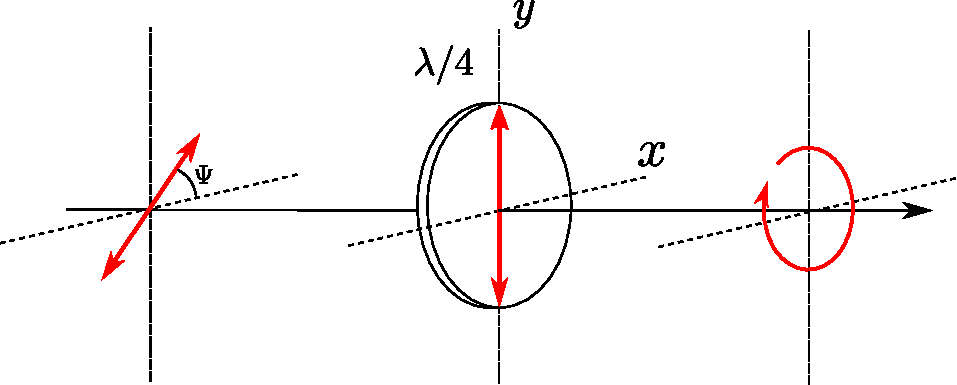
\includegraphics[scale=.7]{qwp_retarder}
\caption[Generación de estados de polarización circulares]{Propagación de un estado de polarización lineal a
  $45^{\circ}$ a través de una placa de retardo de cuarto de onda
  vertical que genera un estado de polarización circular derecho. Las
placas de cuarto de onda introducen un retardo de fase de
$\frac{\pi}{2}$ radianes.}
\label{fig:qwp_retarder}
\end{figure}
La operación correspondiente en el formalismo de Jones es,
\begin{align*}
\mathbf{CD} &=
R^{T}\left(\frac{\pi}{2}\right)\left(QWP\right)R\left(\frac{\pi}{2}\right)\mathbf{45}^{\circ},\\ 
  \frac{1}{\sqrt{2}}
\begin{pmatrix}
1\\i
\end{pmatrix}&=
\begin{pmatrix}
  0 &-1\\1&0
\end{pmatrix}
\begin{pmatrix} e^{i\frac{\pi}{4}}  &0\\0&e^{-i\frac{\pi}{4}} \end{pmatrix}
\begin{pmatrix}
  0&1\\-1&0
\end{pmatrix}
 \frac{1}{\sqrt{2}}
\begin{pmatrix}
1\\ 1
\end{pmatrix},
\\
&=
\begin{pmatrix}
e^{-i\frac{\pi}{4}}  & 0 \\0 & e^{i\frac{\pi}{4}} 
\end{pmatrix}
  \frac{1}{\sqrt{2}}
\begin{pmatrix}
1\\ 1
\end{pmatrix},\\
&=
\begin{pmatrix}
1  & 0 \\0 & i
\end{pmatrix}
  \frac{1}{\sqrt{2}}
\begin{pmatrix}
1\\ 1
\end{pmatrix}.
\end{align*}
En cambio, los retardadores de media onda permiten rotar el estado de
polarización sin afectar la intensidad a la salida. En la
figura \ref{fig:hwp_retarder} se muestra cómo una placa de media onda
orientada a $45^{\circ}$ puede rotar un estado de polarización lineal
horizontal a uno vertical. 
\begin{figure}[h!]
\centering
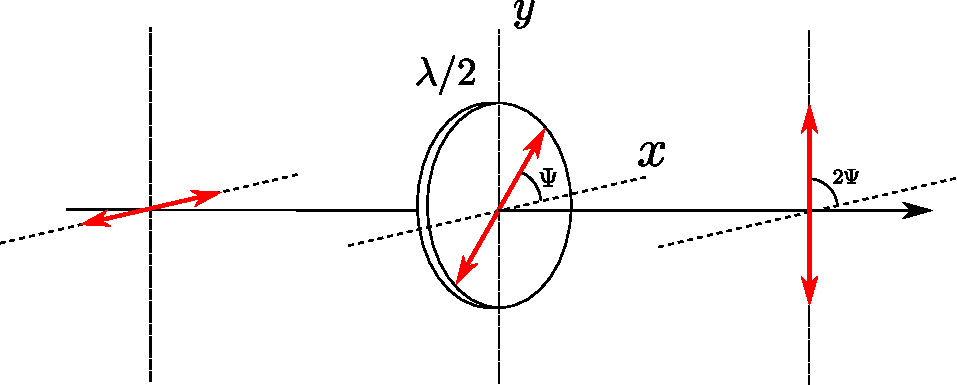
\includegraphics[scale=.7]{HWP_retarder}
\caption[Generación de estados de polarización lineales]{Propagación de un estado de polarización lineal horizontal a través de una placa de retardo de media onda
  vertical a $45^{\circ}$ que genera un estado de polarización lineal vertical. Las
placas de media onda introducen un retardo de fase de
$\pi$ radianes.}
\label{fig:hwp_retarder}
\end{figure}
Como en los casos anteriores, se puede representar la rotación de la
polarización usando el formalismo de Jones:
\begin{align*}
\mathbf{V} &=
R^{T}\left(\frac{\pi}{4}\right)\left(HWP\right)R\left(\frac{\pi}{4}\right)\mathbf{H},\\ 
\begin{pmatrix}
0\\1
\end{pmatrix}&=
 \frac{1}{\sqrt{2}}
\begin{pmatrix}
  1 &-1\\1&1
\end{pmatrix}
\begin{pmatrix} 1
  &0\\0&-1 \end{pmatrix}
 \frac{1}{\sqrt{2}}
\begin{pmatrix}
1&1\\-1&1
\end{pmatrix}
\begin{pmatrix}
1\\ 0
\end{pmatrix},
\\
&=
\begin{pmatrix}
0  & 1 \\1 & 0
\end{pmatrix}
\begin{pmatrix}
1\\ 0
\end{pmatrix},\\&=
\begin{pmatrix}
0\\1
\end{pmatrix}.
\end{align*}
Combinando rotadores ópticos (HWP) y retardadores de cuarto de onda
(QWP), 
podemos generar polarizaciones elípticas con cualquier inclinación y
elipticidad. Así como estos elementos pueden ser modelados por una
matriz, el SLM, que es también un elemento birrefringente que
transforma los estados de polarización puede ser modelado con matrices
de Jones que cumplen las mismas propiedades generales. 
% Esto será de utilidad más adelante pues los autovectores
% de las matrices de Jones indican los estados de polarización para los
% cuales el sistema es transparente, es decir, no se modifica el vector
% tras la operación de la matriz,
% \[\mathbf{M}J_{\lambda} = \lambda J_{\lambda}.\]
% Cuando se desea modulación de sólo fase en un SLM lo que se busca es
% precisamente que no se modifique la polarización y por ende la
% amplitud. El problema de calibrar moduladores se reduce a encontrar la
% matriz que define el LC y extraer sus autoestados tal y como dicen
% Pezzanitti y Davis en \citepChGen{Pezzaniti1993,Davis1998,Davis2003}.
En la sección que sigue se construirá un modelo para describir el
comportamiento de un cristal líquido enroscado (TN-LCD) en términos de
matrices de Jones.

\subsection{Propiedades ópticas de los cristales líquidos nemáticos enroscados (TN-LCD)}
\label{sec:Propiedades_opticas_de_TNLCD}
Los cristales líquidos del tipo TN-LCD son medios ópticos inhomogeneos
y anisotrópicos que localmente actúan como si fueran cristales
birrefringentes uniaxiales con su eje óptico orientado en la dirección
preferente de las moléculas. Como se mencionó en la sección
\ref{sec:LC-clasification} la anisotropía se debe a la forma obloide
de las moléculas del cristal, y en el caso de los TN la inhomogeneidad
viene dada por la orientación preferencial de las moléculas que es
función de su posición. Las propiedades ópticas se estudian suponiendo
que el material se puede representar como láminas delgadas perpendiculares a la
dirección de propagación, cada una de ellas actuando como si fuera un
cristal birrefringente uniaxial con su eje óptico rotado respecto al eje $x$ un ángulo
$\psi$ como se ilustra en la Fig.~\ref{fig:tn-lcd_sticks}.  
\begin{figure}[h!]
\centering
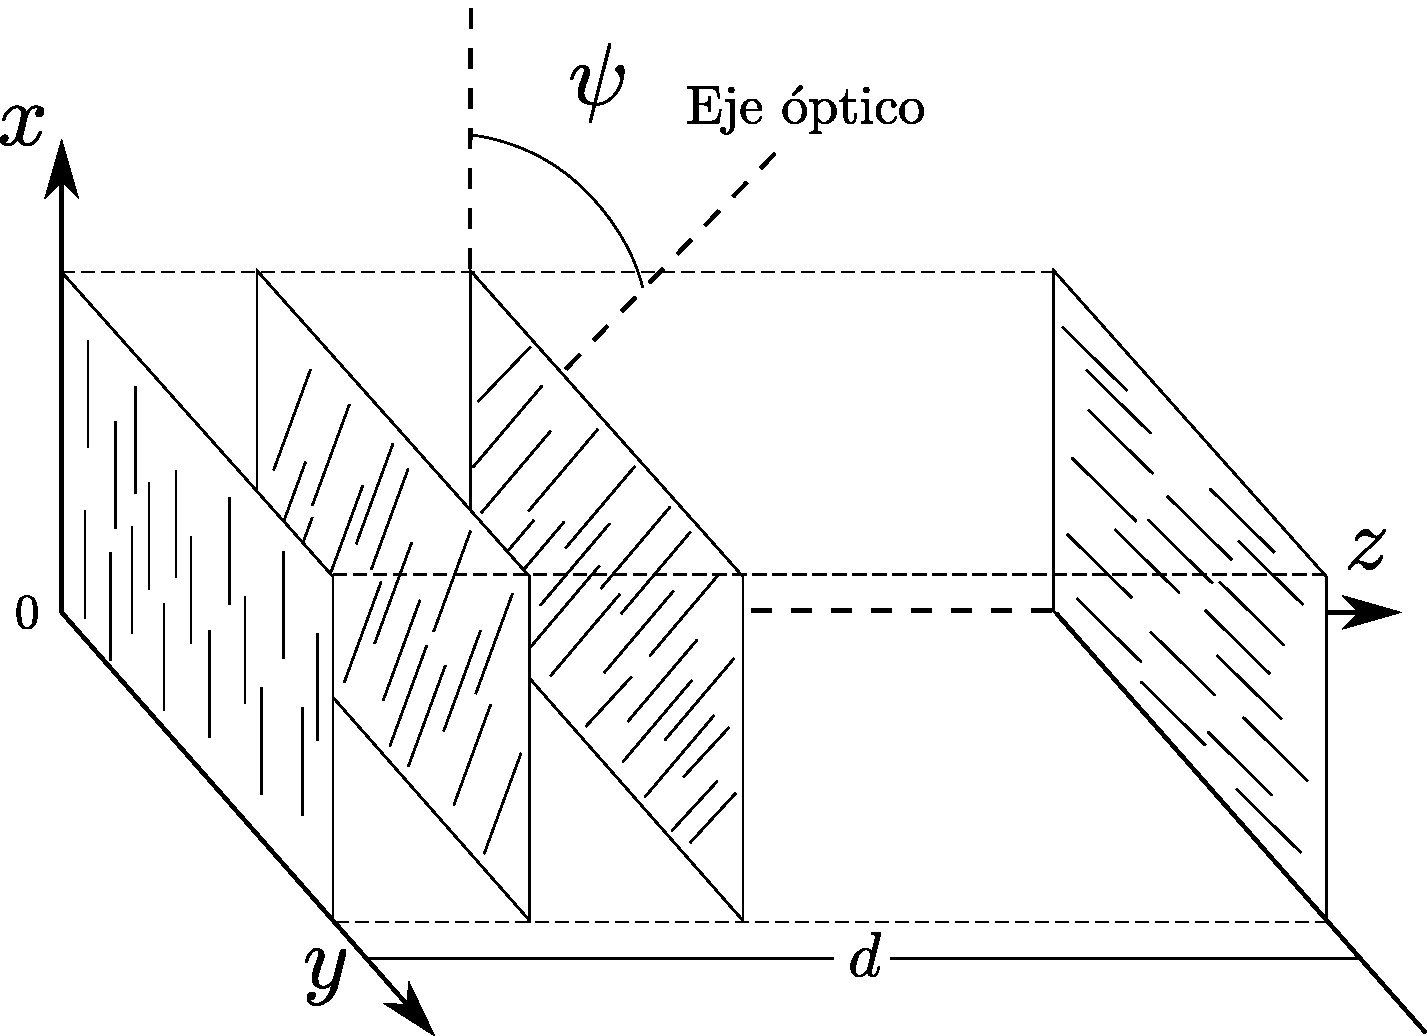
\includegraphics[scale = .3]{TN-LCD_sticks}
\caption[Propagación de la luz en un TN-LC]{Propagación de la luz en
  un cristal líquido del tipo Twisted 
  Nematic. En este diagrama el ángulo de entorchado es de $90^{\circ}$.}
\label{fig:tn-lcd_sticks}
\end{figure}
La rotación de cada \textit{lámina} de
moléculas se asume proporcional a la distancia desde la superficie de
entra da del LCD \citepChGen{Yariv2002},
\begin{equation}
  \label{eq:twist_angle}
\psi(z)  =\alpha z.  
\end{equation}
Aquí la constante $\alpha$
se conoce como coeficiente de torsión, y el ángulo a la salida viene
dado por $$\phi \equiv \psi(d)=\alpha d.$$ Si se divide el cristal en
$N$ láminas, cada una tendrá un grosor $d/N$ y estará orientada en los ángulos
$\rho,2\rho,3\rho,\dots\left(N-1\right)\rho,N\rho$ con
$\rho=\phi/N$. Si cada lámina representa un cristal birrefringente, ésta tendrá una
birrefringencia asociada a su grosor dada por $$\beta_N = \frac{\pi
  d}{2N}\left(n_e-n_o\right).$$
La matriz de Jones general para el conjunto de todas las láminas se
encuentra como la multiplicación de cada una como se muestra a
continuación:
\[ M= W_NW_{N-1}\cdots W_3W_2W_1=\prod_{m=1}^NW_m = \prod_{m=1}^NR(m\rho)^TW_0R(m\rho), \]
dónde $R$ es la matriz de rotación, $W_m$ es la matriz de Jones para
el retardador $m$ rotada, y $W_0$ es aquella lámina en donde el eje rápido está
orientado con el eje $x$,
\begin{equation*}
W_0 =
\begin{pmatrix}
  e^{i\beta/2N} &0 \\ 0 & e^{-i\beta/2N} 
\end{pmatrix}.
\end{equation*}
Las matrices de rotación cumplen la siguiente regla:
\begin{align*}
R^T(\psi_m)R^T(\psi_{m-1}) &= R^T\left(\psi_m+\psi_{m-1}\right),\\
&=
\begin{pmatrix}
  \cos{\psi_m}&  -\sin{\psi_m}\\  \sin{\psi_m}&  \cos{\psi_m}
\end{pmatrix}
\begin{pmatrix}
  \cos{\psi_{m-1}}&  -\sin{\psi_{m-1}}\\  \sin{\psi_{m-1}}&  \cos{\psi_{m-1}}
\end{pmatrix},\\
&=
\begin{pmatrix}
  \cos{\psi_m}\cos{\psi_{m-1}}-\sin{\psi_m}\sin{\psi_{m-1}}&  
-(\cos{\psi_m}\sin{\psi_{m-1}}+\sin{\psi_m} \cos{\psi_{m-1}})\\
  \sin{\psi_m} \cos{\psi_{m-1}}+\cos{\psi_m}\sin{\psi_{m-1}}& 
 -\sin{\psi_m}\sin{\psi_{m-1}}+\cos{\psi_m}\cos{\psi_{m-1}}
\end{pmatrix},  \\
&=\begin{pmatrix}
  \cos{\left(\psi_m+\psi_{m-1}\right)}&  -\sin{\left(\psi_m+\psi_{m-1}\right)}\\
  \sin{\left(\psi_m+\psi_{m-1}\right)}&  \cos{\left(\psi_m+\psi_{m-1}\right)} 
\end{pmatrix}.
\end{align*}
Usando esta propiedad de las matrices de rotación, se puede seguir el
siguiente razonamiento, si $N=1$ entonces,
\begin{equation*}
  M = R^T(\rho)W_0R(\rho).
\end{equation*}
Si en cambio $N=2$ se tiene
\begin{align*}
  M &= R^T(2\rho)W_0R(2\rho)R^T(\rho)W_0R(\rho),\\
      &=R^T(2\rho)W_0R(\rho)R(\rho)R^T(\rho)W_0R(\rho).
\end{align*}
Como $R(\rho)R^T(\rho)=\mathds{1}$ entonces,
\begin{align*}
 M &= R^T(2\rho)W_0R(\rho)W_0R(\rho),\\
     &=R^T(2\rho)\left[W_0R(\rho)\right]^2.
\end{align*}
Y para $N=3$:
\begin{align*}
  M &= R^T(3\rho)W_0R(3\rho)R^T(2\rho)W_0R(2\rho)R^T(\rho)W_0R(\rho),\\
      &=R^T(3\rho)W_0R(3\rho)R^T(2\rho)\left[W_0R(\rho)\right]^2,\\
      &=R^T(3\rho)W_0R(\rho)R(2\rho)R^T(2\rho)\left[W_0R(\rho)\right]^2,\\
      &=R^T(3\rho)W_0R(\rho)\left[W_0R(\rho)\right]^2,\\
      &=R^T(3\rho)\left[W_0R(\rho)\right]^3.
\end{align*}
Ahora, para una cantidad arbitraria $m$:
\begin{align*}
  M &= R^T(m\rho)W_0R(m\rho)R^T((m-1)\rho)\left[W_0R(\rho)\right]^{m-1},\\
      &=R^T(m\rho)W_0R(\rho)R((m-1)\rho)R^T((m-1)\rho)\left[W_0R(\rho)\right]^{m-1},\\  
      &=R^T(m\rho)W_0R(\rho)\left[W_0R(\rho)\right]^{m-1},\\
      &=R^T(m\rho)\left[W_0R(m\rho)\right]^{m}.
\end{align*}
Y así se obtiene la matriz general del TN-LCD según \citetChGen{Yariv2002} en
términos de dos matrices, una que cambia el estado de polarización y
otra que simplemente lo rota
\begin{align}
M&=R^T\left( \phi\right)
\left[W_0R\left(\frac{\phi}{N}\right)\right]^N,\\
&=R^T\left( \phi\right)
\begin{pmatrix}
  \cos{\frac{\phi}{N}e^{i\beta/N}} &  \sin{\frac{\phi}{N}e^{i\beta/N}}\\
  -\sin{\frac{\phi}{N}e^{-i\beta/N}} &  \cos{\frac{\phi}{N}e^{-i\beta/N}}  
\end{pmatrix}^N.
\label{eq:general_lcd_matrix}
\end{align}
La Eq.~(\ref{eq:general_lcd_matrix}) puede ser simplificada aún
mas como muestran \citetChGen{Yeh1999} si se usa la identidad de Chebyshev
para matrices unimodulares  
\begin{equation}
  \begin{pmatrix}
    A & B \\ C & D
  \end{pmatrix}^m
=
\begin{pmatrix}
  \frac{A\sin{ (mZ) }-\sin(m-1)Z }{\sin{Z} }
  &\frac{B\sin{(mZ)}}{\sin{Z}}\\
\frac{C\sin{(mZ)}}{\sin{Z}}&   \frac{D\sin{ (mZ) }-\sin(m-1)Z }{\sin{Z} }
\end{pmatrix},
  \label{eq:chebyshev}
\end{equation}
con \[Z = \cos^{-1}{\left[\frac{1}{2}(A+D)\right]}.\]
Si se saca el límite cuando $(N\rightarrow \infty)$
\citetChGen{Saleh1990} muestran que se puede obtener la
siguiente matriz,
\begin{equation}
  \label{eq:TN-LCD_Jones_Matrix}
  M=
  \begin{pmatrix}
    \cos{\phi} & -\sin{\phi}\\\sin{\phi}&\cos{\phi}
  \end{pmatrix}
  \begin{pmatrix}
    \cos{\gamma}+i\beta\frac{\sin{\gamma}}{\gamma} & \phi\frac{\sin{\gamma}}{\gamma}\\
-\phi\frac{\sin{\gamma}}{\gamma}   & \cos{\gamma}-i\beta\frac{\sin{\gamma}}{\gamma}
  \end{pmatrix},
\end{equation} 
dónde
\[\gamma=\sqrt{\phi^2+\beta^2}.\]

Ahora, la matriz de la Eq.~(\ref{eq:TN-LCD_Jones_Matrix})  es la
matriz que todos los autores referenciados en el
estudio del estado del arte usan, y a partir de la cual se basan
para caracterizar moduladores. La matriz que representa un
SLM  tal como se estudió en esta sección es la forma más
simple de representar un cristal líquido del tipo twisted nematic y se
conoce como el modelo de \citetChGen{Saleh1990}. Este modelo
parte de asumir las siguientes aproximaciones:

\begin{itemize}
\item El TN-LCD se comporta como una sucesión de  láminas
  retardadoras en las cuales la orientación del vector director varía
  gradualmente desde un ángulo a la entrada hasta un ángulo a la
  salida y formando un ángulo de rotación conocido como twist angle. 
\item El ángulo de rotación (twist angle) es una función lineal
  proporcional a la profundidad en el cristal tal y como se expresa en
  la Eq.~(\ref{eq:twist_angle}).
\item El ángulo de inclinación (tilt angle) se produce cuando se
  introduce un campo eléctrico que hace rotar las moléculas para
  alinearlas en su dirección. Éste ángulo se asume constante a lo
  largo del cristal para un voltaje específico. Si la birrefringencia
  es proporcional al ángulo de inclinación, entonces al variar el
  voltaje ésta variará linealmente con respecto al voltaje.
\end{itemize}

En modelos posteriores como los de \citetChGen{Coy1996} y
\citetChGen{Marquez2000} se construyen matrices para el LCD que
corrigen comportamientos no lineales no previstos por  Lu y Saleh. El
principal factor a corregir en un LCD es la tendencia de las moléculas
cercanas a las paredes del cristal a conservar la dirección de pulido
de los vidrios que las contienen como se ilustra en la Fig.~\ref{fig:lcd_models}.
\begin{figure}[h!]
\centering
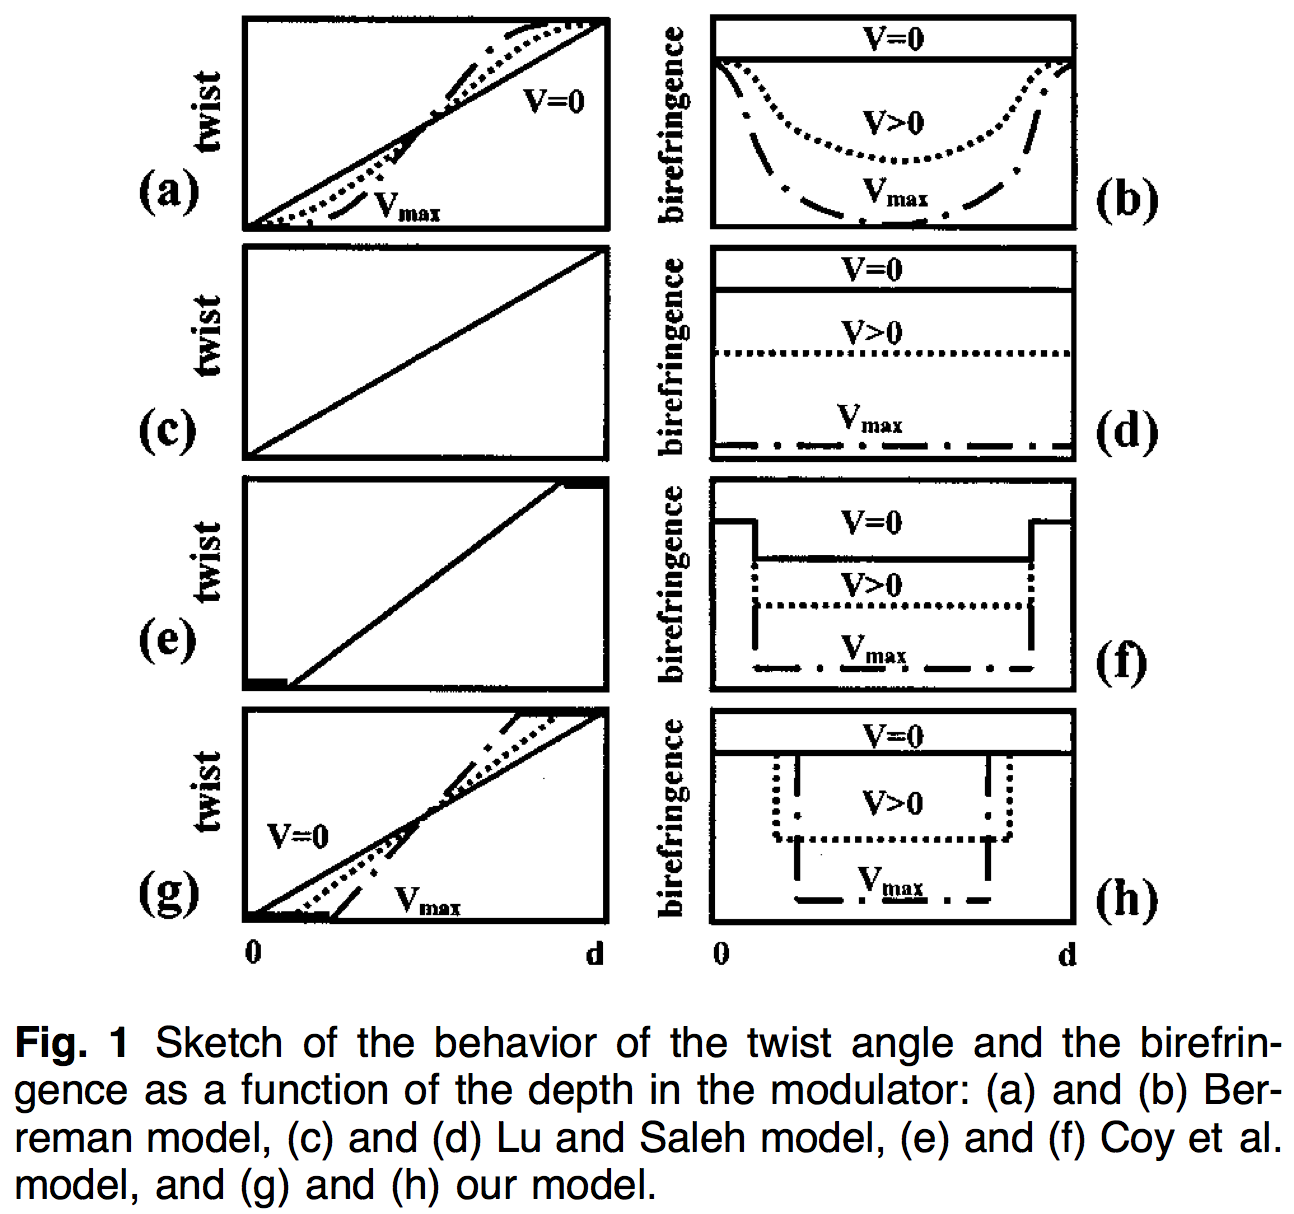
\includegraphics[scale=.5]{lcd_models}
\caption[Modelos de TN-LCD]{Modelos de TN-LCD tomado de \citetChGen{Marquez2000}.}
\label{fig:lcd_models}
\end{figure}
 Este efecto hace que el ángulo de
rotación no sea una función lineal  lo largo de la profundidad y que la
birrefringencia no sea una función lineal del voltaje.

\section{Revisión de la literatura}
Se realizó una revisión de la literatura en el contexto de calibración
de moduladores basados en TN-LCD y se encontró que para poder utilizar
una pantalla de cristal líquido como un modulador de sólo fase se debe
caracterizar el dispositivo como si fuera un elemento óptico que
afecta tanto la polarización como la fase de la luz. La mayoría de los
autores usan el cálculo de Jones para representar el efecto del SLM
sobre la luz como la operación de la matriz del SLM sobre un vector de
polarización a la entrada. Sin embargo, algunos autores como \citetChGen{Yu2012}, \citetChGen{Moreno2008} y Durán et al. \citepChGen{Duran2007} utilizan también
la medida de parámetros de  Stokes y matrices de Muller para obtener
curvas de calibración de los dispositivos. El reto en ambos casos es
encontrar una matriz que 
modele con precisión el comportamiento del modulador para diferentes
valores de voltaje aplicado. 

Hay dos formas básicas de caracterizar el
SLM, por una parte se puede seguir el camino riguroso y analizar el
TN-LCD desde el punto de vista físico como se hizo en la sección
anterior. Para este caso se deben encontrar los parámetros físicos que
determinan la matriz que se presentó en la Eq.~(\ref{eq:TN-LCD_Jones_Matrix}), es decir, la 
birrefringencia como función del voltaje, el ángulo de rotación de las
moléculas a la entrada del modulador, y el ángulo de rotación total
que experimentan las moléculas hasta la salida del modulador. Estos
parámetros son encontrados en la mayoría de los casos por medio de
ajuste de curvas con medidas experimentales de la tramitancia.  La
otra forma en la que se obtiene la matriz de Jones es asumiendo que el
sistema es como una caja negra que debe cumplir reglas menos
exigentes. En la Fig.~\ref{fig:articulos_metodos} se ilustra por
medio de dos columnas la cantidad y fecha en las cuales se han
publicado artículos científicos en donde se usa uno u otro método
para caracterizar los moduladores. Adicionalmente, se identificaron los
grupos que más han publicado sobre el tema. De la Fig.~\ref{fig:articulos_metodos} y de las fechas en los artículos de la
bibliografía se puede observar que la investigación en TN-LCD para
aplicación en procesamiento óptico tuvo su auge entre 1990 y 2010
aproximadamente, esto se debe como afirman \citetChGen{Kirsch1992}
a que a finales de los 80s las pantallas 
de LC para televisores portátiles resultaron interesantes a los
investigadores como dispositivos para generación dinámica de máscaras
de amplitud y fase. El declive en cambio, se debe a que los
moduladores de reflexión han ido reemplazando a los de transmisión por
 no necesitar de una caracterización y tener mejores prestaciones. 
También se ha concluido que los artículos que buscaban encontrar todos los
parámetros del modulador como el de \citetChGen{Marquez2000} y
el de \citetChGen{Zhisheng1998} en 1998 preceden en el tiempo a los artículos
donde se busca simplificar el modelo y asumir el comportamiento del
LCD como una caja negra, como el de \citetChGen{Moreno2003} en 2003, o
como los dos artículos de \citetChGen{Ma2010, Ma2011} en 2010 y
2011, que son en los cuales nos
hemos inspirado para caracterizar nuestros SLMs. Los autores de estas
últimas referencias identificaron una necesidad de 
simplificar el proceso de caracterización, y entre sus argumentos 
están la simplicidad matemática y número reducido de medidas necesarias.
\begin{figure}[h!]
\centering
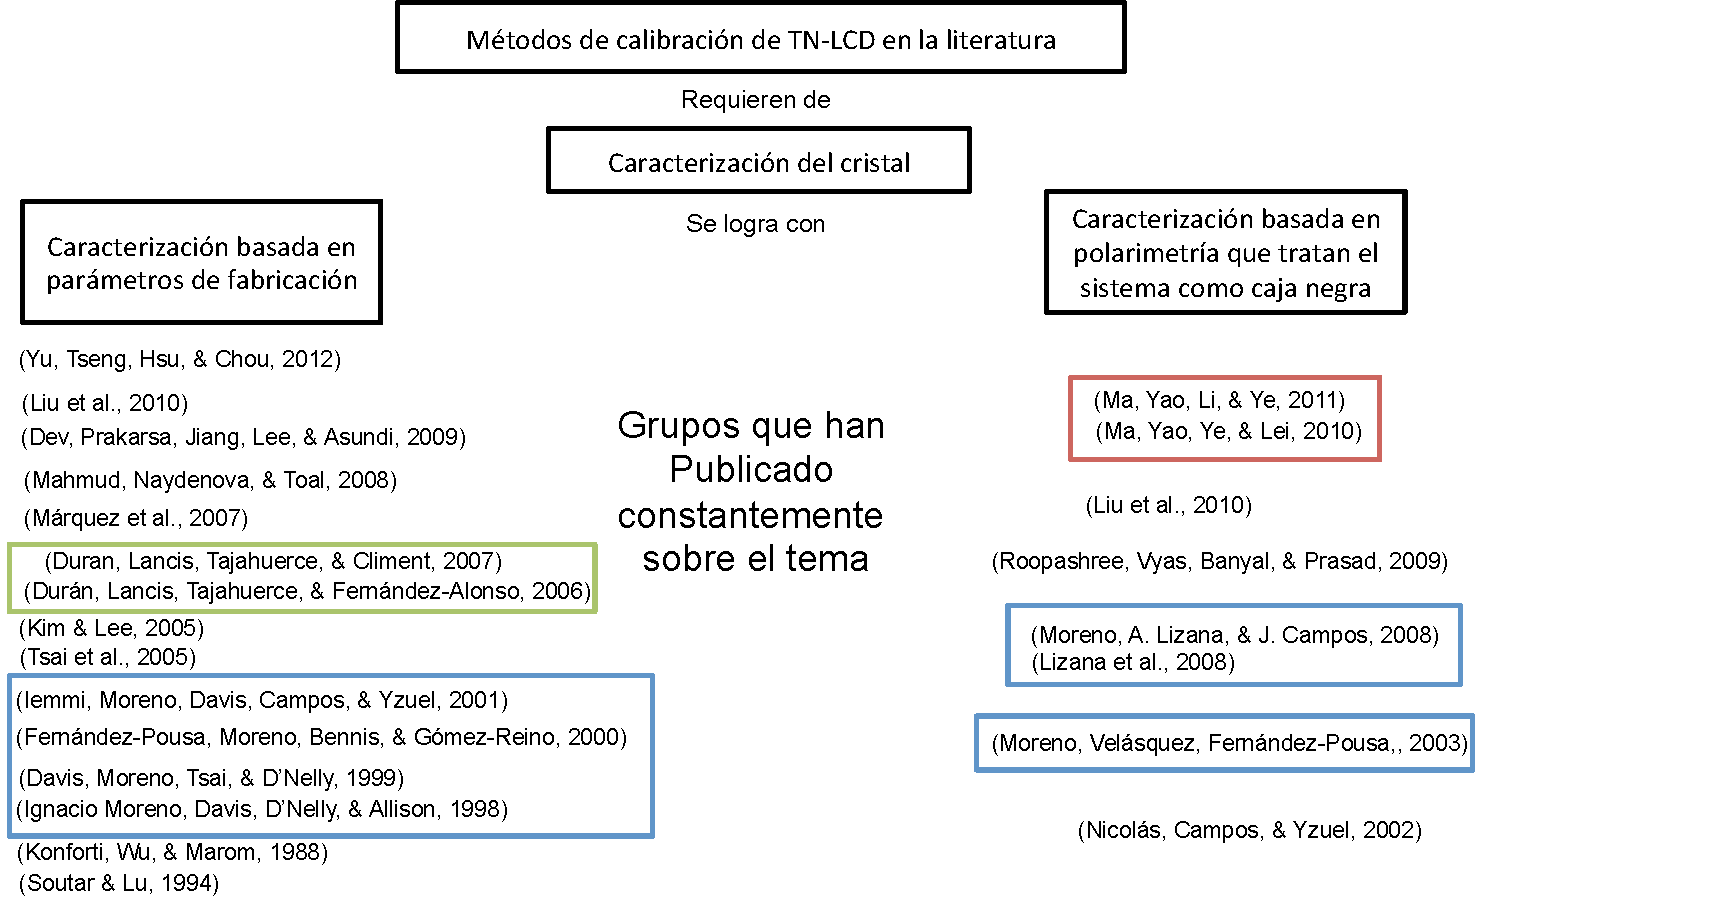
\includegraphics[scale=.6]{articulos_metodos}
\caption[Publicaciones en relación a la caracterización de TN-LCD]{Tabla de publicaciones en relación con caracterización de
  moduladores tipo TN-LCD. Los rectángulos representan los grupos que
  han publicado más en el tema y que resultan de mayor interés para
  este trabajo. }
\label{fig:articulos_metodos}
\end{figure}
El principal resultado del estudio del estado del arte fue encontrar
un patrón en la evolución del tema en la literatura desde los primeros
métodos para pantallas de televisor \citepChGen{Moreno1998} hasta campos
dónde se modula la polarización producidos por moduladores
\citepChGen{Moreno2011}. Este patrón tiene como columna vertebral al 
investigador Ignacio Moreno que, junto con otros investigadores en
universidades de España y California ha dirigido los avances en aplicaciones
científicas de pantallas TN-LCD. 

En lo que sigue de este capítulo presentaremos el resultado de la
caracterizaación de un SLM modelo LC2002 de marca Holoeye con el
método de \citetChGen{Ma2010}.
% una variación del método de caracterización de
% \citetChGen{Moreno2003} implementada por nosotros y que 
%tambien considera el SLM como una caja negra. 
Veremos que la implementación de este método y los resultados
obtenidos involucraron no solo el análisis de datos experimentales sino también el diseño y
construcción de un sistema automatizado para la toma de medidas que se
describe en la sección \ref{sec:instrumento} y el apéndice \ref{AppendixA} 
También se mostrará un método alternativo propuesto por nosotros que
requiere más medidas y permite obtener resultados más veraces. 

Una vez caracterizado el SLM se identificó una combinación de estados
de polarización a la entrada y la salida del SLM que permiten una
modulación de solo fase con la cual se pueden emular elementos
difractivos digitales tales como máscaras espiral de fase, prismas,
lentes de Fresnel e inclusive aberraciones. Los elementos difractivos
producidos de forma digital, y en particular, las máscaras espiral 
 son la clave para producir haces Laguerre-Gauss.  

\chapter{Caracterización de TN-SLM}
\label{cha:Gen_carac}
\label{sec:ChGV_Caracterizacion_de_SLM}
\lhead{Generación de haces Laguerre-Gauss por medio de un SLM: \textit{Caracterización de un TN-SLM}}

Como se mencionó antes, en la caracterización del SLM se pretende
encontrar estados de polarización a la entrada y salida del modulador
que produzcan modulaciones de solo fase, con buena transmitancia y con
un rango amplio de valores de fase. 
Por ende es necesario medir las modulaciones de amplitud y de fase. En
las siguientes secciones se muestra cómo medimos las modulaciones de
amplitud y fase. 

%\subsection{Medida de la modulación de amplitud}
\section{Medida de la modulación de amplitud}
\label{sec:ChGV_med_mod_amp}

En la Fig.~\ref{fig:PSG_PSD} se presenta un esquema del sistema
óptico usado para medir la modulación de amplitud. Si el haz tiene una
polarización lineal y se propaga en la dirección de $z$, la combinación
de un HWP y un primer QWP, conocida como \textbf{generador de estados de
polarización} (\acrshort{PSG}), permite producir estados de polarización
arbitrarios a la entrada del SLM. Luego, el haz llega al SLM y la modulación de amplitud se
debe a que las moléculas de LC en el SLM cambian el estado de
polarización dependiendo del valor de voltaje aplicado. Cuando se añade un \textbf{detector de estados de
polarización} (\acrshort{PSD}) compuesto por un segundo QWP y un polarizador, la amplitud del campo a la salida del polarizador
(P) dependerá de la matriz de Jones del SLM para el nivel de gris
actual y de los vectores de Jones asociados al PSG y PSD. A la salida
del PSD hay un estado con polarización lineal cuya intensidad puede
ser medida usando un fotodetector, o una cámara. 
 \begin{figure}[h!]
\centering
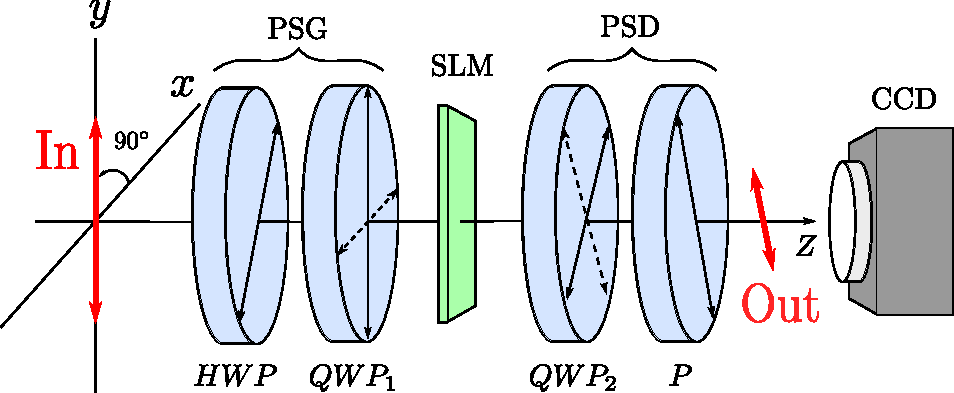
\includegraphics[scale=.8]{PSG_PSD.pdf}
\caption[Esquema de un sistema generador y analizador de estados de
polarización]{Esquema general de un sistema óptico para
  caracterización de modulación de intensidad de un TN-SLM.}
\label{fig:PSG_PSD}
\end{figure}

Desde el punto de vista matemático, el campo a la salida ($Out$) se puede
obtener multiplicando un vector de entrada $In$ por cada uno de
los elementos del sistema 
\begin{equation}
\label{eq:ChGV_Out}
Out = \left( \mathbf{P}\ \mathbf{QWP_2}\ \right) \mathbf{SLM}\ \left( \mathbf{QWP_1}\
\mathbf{HWP}\right)\ In.
\end{equation}
La intensidad medida por la cámara no es más que el módulo cuadrado de
este campo,

\begin{equation}
I = |Out|^2 = Out^{\dagger}Out.
\end{equation}

Luego, en la Fig. \ref{fig:amp_H_V_SLM_2002} se presenta
una curva de modulación de amplitud que se consigue graficando los
valores de intensidad normalizada cuando se varían los niveles de gris discretos
del SLM de 0 a 255. Como se mencionó antes, el nivel de gris es
proporcional al voltaje sobre las celdas de CL y corresponde a 0
cuando el ángulo de inclinación de las moléculas es de 90º con
respecto a la dirección de propagación. La
Fig.~\ref{fig:amp_H_V_SLM_2002} es especialmente interesante porque
muestra el comportamiento del SLM marca Holoeye modelo LC2002 en la
configuración típica de pantallas LCD para proyección, es decir, cuando
el PSG genera un estado de polarización a la entrada vertical y el
PSD detecta un estado horizontal. Como es de esperarse, en esta
configuración el SLM modula amplitud en un rango de 0 a 1 y con una
pendiente relativamente suave y lineal. 
\begin{figure}[h!]
\centering
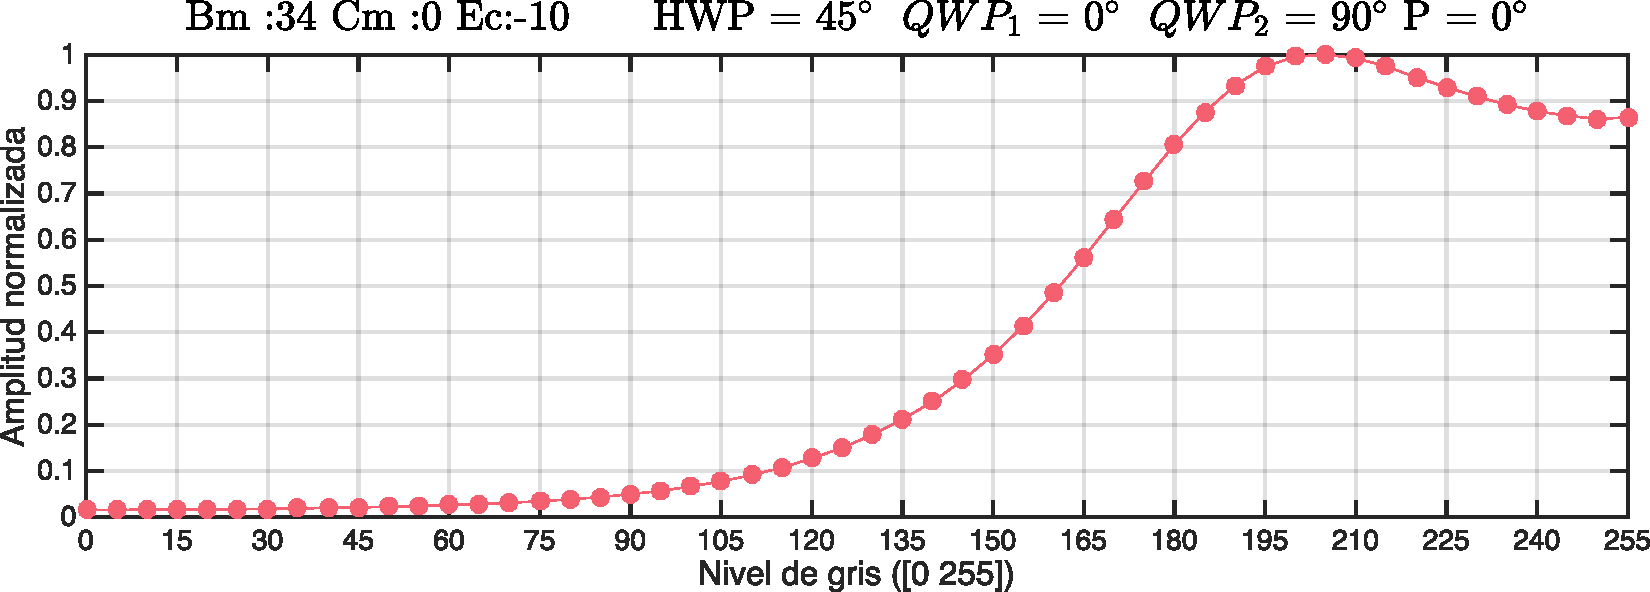
\includegraphics[scale=.55]{amp_H_V_SLM_2002.pdf}
\caption[Curva de modulación de amplitud para un estado no
óptimo]{Medida de la intensidad normalizada del SLM Holoeye LC-2002 en la configuración típica
  de pantallas LCD para proyección. Los primeros tres valores de la parte superior indican la
configuración de brillo (Bm) y contraste (Cm) del SLM, así como la
exposición de la cámara (Ec). Los siguientes 4 indican las posiciones
de los elementos ópticos usados para generar y detectar
estados de polarización.}
\label{fig:amp_H_V_SLM_2002}
\end{figure}
Este tipo de modulaciónes
sirven para proyectar imágenes en niveles de gris y se pueden lograr
con dos polarizadores como PSG y PSD que generen estados lineales ortogonales
entre si.
% Como se explicó en la sección \ref{sec:Propiedades_opticas_de_TNLCD}
%  si el ángulo de torsión de las moléculas en el SLM es de $90^{\circ}$ y
% las moléculas a la entrada están alineadas con el eje horizontal, el
% estado de polarización a la salida será aproximadamente vertical.
No obstante, nuestro objetivo es encontrar una combinación de estados
de polarización que resulten en una baja modulación de amplitud y
buena transmitancia. 

% \subsection{Medida de múltiples estados para alimentar un modelo de
%  caja negra.}
%\label{sec:ChGV_med_mod_amp}
La curva de la Fig. \ref{fig:amp_H_V_SLM_2002} caracteriza la modulación de amplitud del SLM para
una sola combinación de PSG y PSD. Una forma de buscar buenas
combinaciones de PSG y PSD consiste en plantear muchos estados
distintos y medir la modulación hasta encontrar un estado que produzca
los efectos deseados. Hacer esto experimentalmente es un proceso
engorroso y requiere de mucho tiempo porque hay muchas combinaciones
posibles que implican rotar elementos ópticos de forma precisa y con
alta repetibilidad. 
En cambio, vamos a medir experimentalmente sólo 6 combinaciones de PSG
y PSD propuestas por \citetChGen{Ma2010} y con
ellas alimentaremos un modelo analítico y otro modelo numérico con los
cuales se obtienen los parámetros de la matriz de 
Jones para cada nivel de gris por medio de operaciones aritméticas
simples en el caso del primero, y funciones de minimización en el segundo.
% serán encontrada por un método de ajuste
% de parámetros.
% de caja negra 
% basado en un algoritmo de minimización basado en la búsqueda del
% gradiente. 
Una vez conocido el modelo del SLM se puede buscar el
estado que mejor satisface las condiciones de operación haciendo simulaciones con
las cuales sí es práctico hacer una búsqueda entre múltiples estados.

A continuación se introducirá una notación alternativa para la
representación de estados de polarización que es de uso generalizada
en las referencias consultadas \citepChGen{Moreno2003,Ma2010} (entre
otras) y que facilita la
representación de las combinaciones de PSG y PSD para medidas de
intensidad.  

%\subsubsection{La notación de Dirac}
\subsection{La notación de Dirac}
De forma similar a cómo sucede en la mecánica cuántica, los estados de
polarización arbitrarios generados por un PSG se pueden representar en
la notación de BraKets de Dirac como Ket's:
\begin{equation}
|J> = \begin{pmatrix} J_x \\ J_y\end{pmatrix} = \left( \mathbf{QWP_1}\
\mathbf{HWP}\right)\ In.
\end{equation}
Y siguiendo esta interpretación, el PSD correspondiente a un PSG dado
es el Bra, es decir, el vector que es complejo conjugado de un Ket
\begin{equation}
<J|= |J>^{\dagger} = \begin{pmatrix} J_x^* &  J_y^*\end{pmatrix}. 
\end{equation}
Por otra parte, la matriz de Jones del SLM cumple el papel que tendría un
operador en la mecánica cuántica. Si los Bra y Ket representan vectores normalizados, la
intensidad del campo a la salida puede ser obtenida como el módulo
cuadrado del valor
esperado del operador del SLM  (Eq. \ref{eq:general_jones_matrix})
cuando la base del PSG es proyectada sobre la del PSD \citepChGen{Moreno2003,Ma2010}.
\begin{align}
\label{eq:valor_esperado}
I = |<J|\mathbf{SLM} |J>|^2 &= 
\begin{pmatrix}
J_x & J_y
\end{pmatrix}
\begin{pmatrix}
A & B\\
 -B^* & A^* 
\end{pmatrix}
\begin{pmatrix}
J_x \\ J_y
\end{pmatrix}
,\nonumber\\
&= 
\begin{pmatrix}
J_x & J_y
\end{pmatrix}
\begin{pmatrix}
X+iY & Z+iW\\
 -Z+iW & X-iY 
\end{pmatrix}
\begin{pmatrix}
J_x \\ J_y
\end{pmatrix}
.
\end{align}
%donde $A$ y $B$ son números complejos.

La intensidad es una variable que se puede medir con una cámara o fotodiodo, y los vectores
correspondientes a los estados producidos por el PSG y el PSD son
conocidos. Como los vectores de Jones que utilizamos están
normalizados, lo más adecuado es normalizar también las medidas de
intensidad. Una forma de normalizar las medidas consiste en medir no
solo el BraKet deseado sino también un Braket en el cual el Bra o PSD es un
vector ortogonal al PSD original.  La intensidad medida con el PSD
ortogonal es entonces un complemento de la original y su suma debe ser
un valor constante. Si se divide cualquiera de las dos intensidades experimentales
sobre la suma de las dos, obtenemos un valor que ha sido
normalizado y que es equivalente a aquellos obtenidos usando del producto
analítico de la Eq. \ref{eq:valor_esperado}, 

\begin{align*}
\hat{I} &= \frac{I}{I+I^{\perp}},&\hat{I}^{\perp} &= \frac{I^{\perp}}{I+I^{\perp}}.
\end{align*}

%\subsubsection{El método de Ma et al.}
\section{El método de Ma et al.~ para la caracterización del SLM}
\label{sec:metodo_ma}
Según \citetChGen{Ma2010}, hay tres combinaciones de PSD y PSG a partir
de las cuales se pueden encontrar los valores X,Y,Z, y W de la matriz
de Jones de un SLM. Si para
normalizar cada una de ellas requerimos medir otra en la cual el Bra
es el vector ortogonal del Bra original, se requiere de las siguientes
6 medidas, 
\begin{align*}
I_1 &= |<\mathbf{H}|SLM|\mathbf{H}>|^2,& I_2 &= |<\mathbf{CD}|SLM|\mathbf{CD}>|^2,&I_3
  &= |<\mathbf{45^{\circ}}|SLM|\mathbf{45^{\circ}}>|^2,\\
I_1^{\perp} &= |<\mathbf{V}|SLM|\mathbf{H}>|^2,&I_2^{\perp} &= |<\mathbf{CI}|SLM|\mathbf{CD}>|^2,&I_{3}^{\perp} &= |<\mathbf{-45^{\circ}}|SLM|\mathbf{45^{\circ}}>|^2.
\end{align*}
Dónde el símbolo $^{\perp}$ denota ortogonalidad, y básicamente se
está midiendo qué tan transparente es el SLM ante 
los estados vertical, circular derecho, y lineal a $45^{\circ}$. 
Estas tres medidas son interesantes porque se puede encontrar una
relación entre la intensidad medida 
y los valores desconocidos de la matriz de Jones. 
A continuación se muestra el procedimiento matemático expuesto por Ma
et al.~que relaciona cada una de las intensidades con los valores de
la matriz de Jones. 
Analizar la transmitancia ante el estado lineal horizontal entrega un valor
de intensidad que es función de $X$ y $Y$,
\begin{align*}
I_1 = |<\mathbf{H}|SLM|\mathbf{H}>|^2 &= X^2+Y^2,\\
&=  \left|\begin{pmatrix} 1&0\end{pmatrix} 
       \begin{pmatrix}
         X+iY & Z+iW \\-Z+iW & X-iY
       \end{pmatrix} \begin{pmatrix}1\\0\end{pmatrix}\right|^2, \\
&=  \left|\begin{pmatrix} 1&0\end{pmatrix} 
       \begin{pmatrix} X+iY \\-Z+iW \end{pmatrix} \right|^2, \\
&=  \left|X+iY\right|^2 =  X^2+Y^2.\\
\end{align*}
Y analizar la transmitancia ante un estado circular derecho entrega un
valor de intensidad función de $X$ y $Z$.
\begin{align*}
I_2 = |<\mathbf{CD}|SLM|\mathbf{CD}>|^2 &= X^2+Z^2,\\
&=  \left|\frac{1}{\sqrt{2}}\begin{pmatrix} 1&-i\end{pmatrix} 
       \begin{pmatrix}
         X+iY & Z+iW \\-Z+iW & X-iY
       \end{pmatrix} \frac{1}{\sqrt{2}}\begin{pmatrix}1\\i\end{pmatrix}\right|^2 ,\\
&=  \left|\frac{1}{2}\begin{pmatrix} 1&-i\end{pmatrix} 
       \begin{pmatrix} X+iY +iZ-W\\-Z+iW +iX+Y\end{pmatrix} \right|^2 ,\\
&=  \left|\frac{1}{2}\left(X+iY+iZ-iW+iZ+W+X-iY\right)\right|^2 =  X^2+Z^2.\\
\end{align*}
Como en los casos anteriores, se muestra que la intensidad medida
cuando se genera y detecta un estado inclinado a $45^{\circ}$ depende
ahora de $X$ y $W$.
\begin{align*}
I_3 = |<\mathbf{45^{\circ}}|SLM|\mathbf{45^{\circ}}>|^2 &= X^2+W^2,\\
&=  \left|\frac{1}{\sqrt{2}}\begin{pmatrix} 1&1\end{pmatrix} 
       \begin{pmatrix}
         X+iY & Z+iW \\-Z+iW & X-iY
       \end{pmatrix} \frac{1}{\sqrt{2}}\begin{pmatrix}1\\1\end{pmatrix}\right|^2 ,\\
&=  \left|\frac{1}{2}\begin{pmatrix} 1&1\end{pmatrix} 
       \begin{pmatrix} X+iY +Z+iW\\-Z+iW +X-iY\end{pmatrix} \right|^2, \\
&=  \left|\frac{1}{2}\left(X+iY+Z+iW-Z+iW+X-iY\right)\right|^2 =  X^2+W^2.\\
\end{align*}
Adicionalmente, de la Eq. \ref{eq:unimodular} podemos deducir la siguiente condición de
normalización que está relacionada con el hecho de ser una matriz
unitaria y por ende unimodular,
\begin{equation*}
X^2+Y^2+Z^2+W^2 =1.
\end{equation*}
Con esta última relación tenemos 4 ecuaciones para 4 incógnitas, y
tras realizar operaciones simples de sustitución podemos despejar
$X^2$, $Y^2$, $Z^2$ y $W^2$ en función de $I_1$, $I_2$, y $I_3$,
\begin{align*}
X^2 &= \frac{1}{2}\left( I_1+I_2+I_3-1\right), & Y^2 &=
                                                       \frac{1}{2}\left(
                                                       I_1-I_2-I_3+1\right),\\
Z^2 &= \frac{1}{2}\left( I_2-I_1-I_3+1\right), & W^2 &=
                                                       \frac{1}{2}\left(
                                                       I_3-I_1-I_2+1\right).\\
\end{align*}

Nosotros medimos estas tres intensidades para 52 de los 255 niveles de
gris del SLM y obtuvimos curvas muy similares a las de \citetChGen{Ma2014}. La
comparación entre las medidas de intensidad normalizadas y las de Ma se observa en la
Fig. \ref{fig:Ma_and_our_Is}.
\begin{figure}[h!]
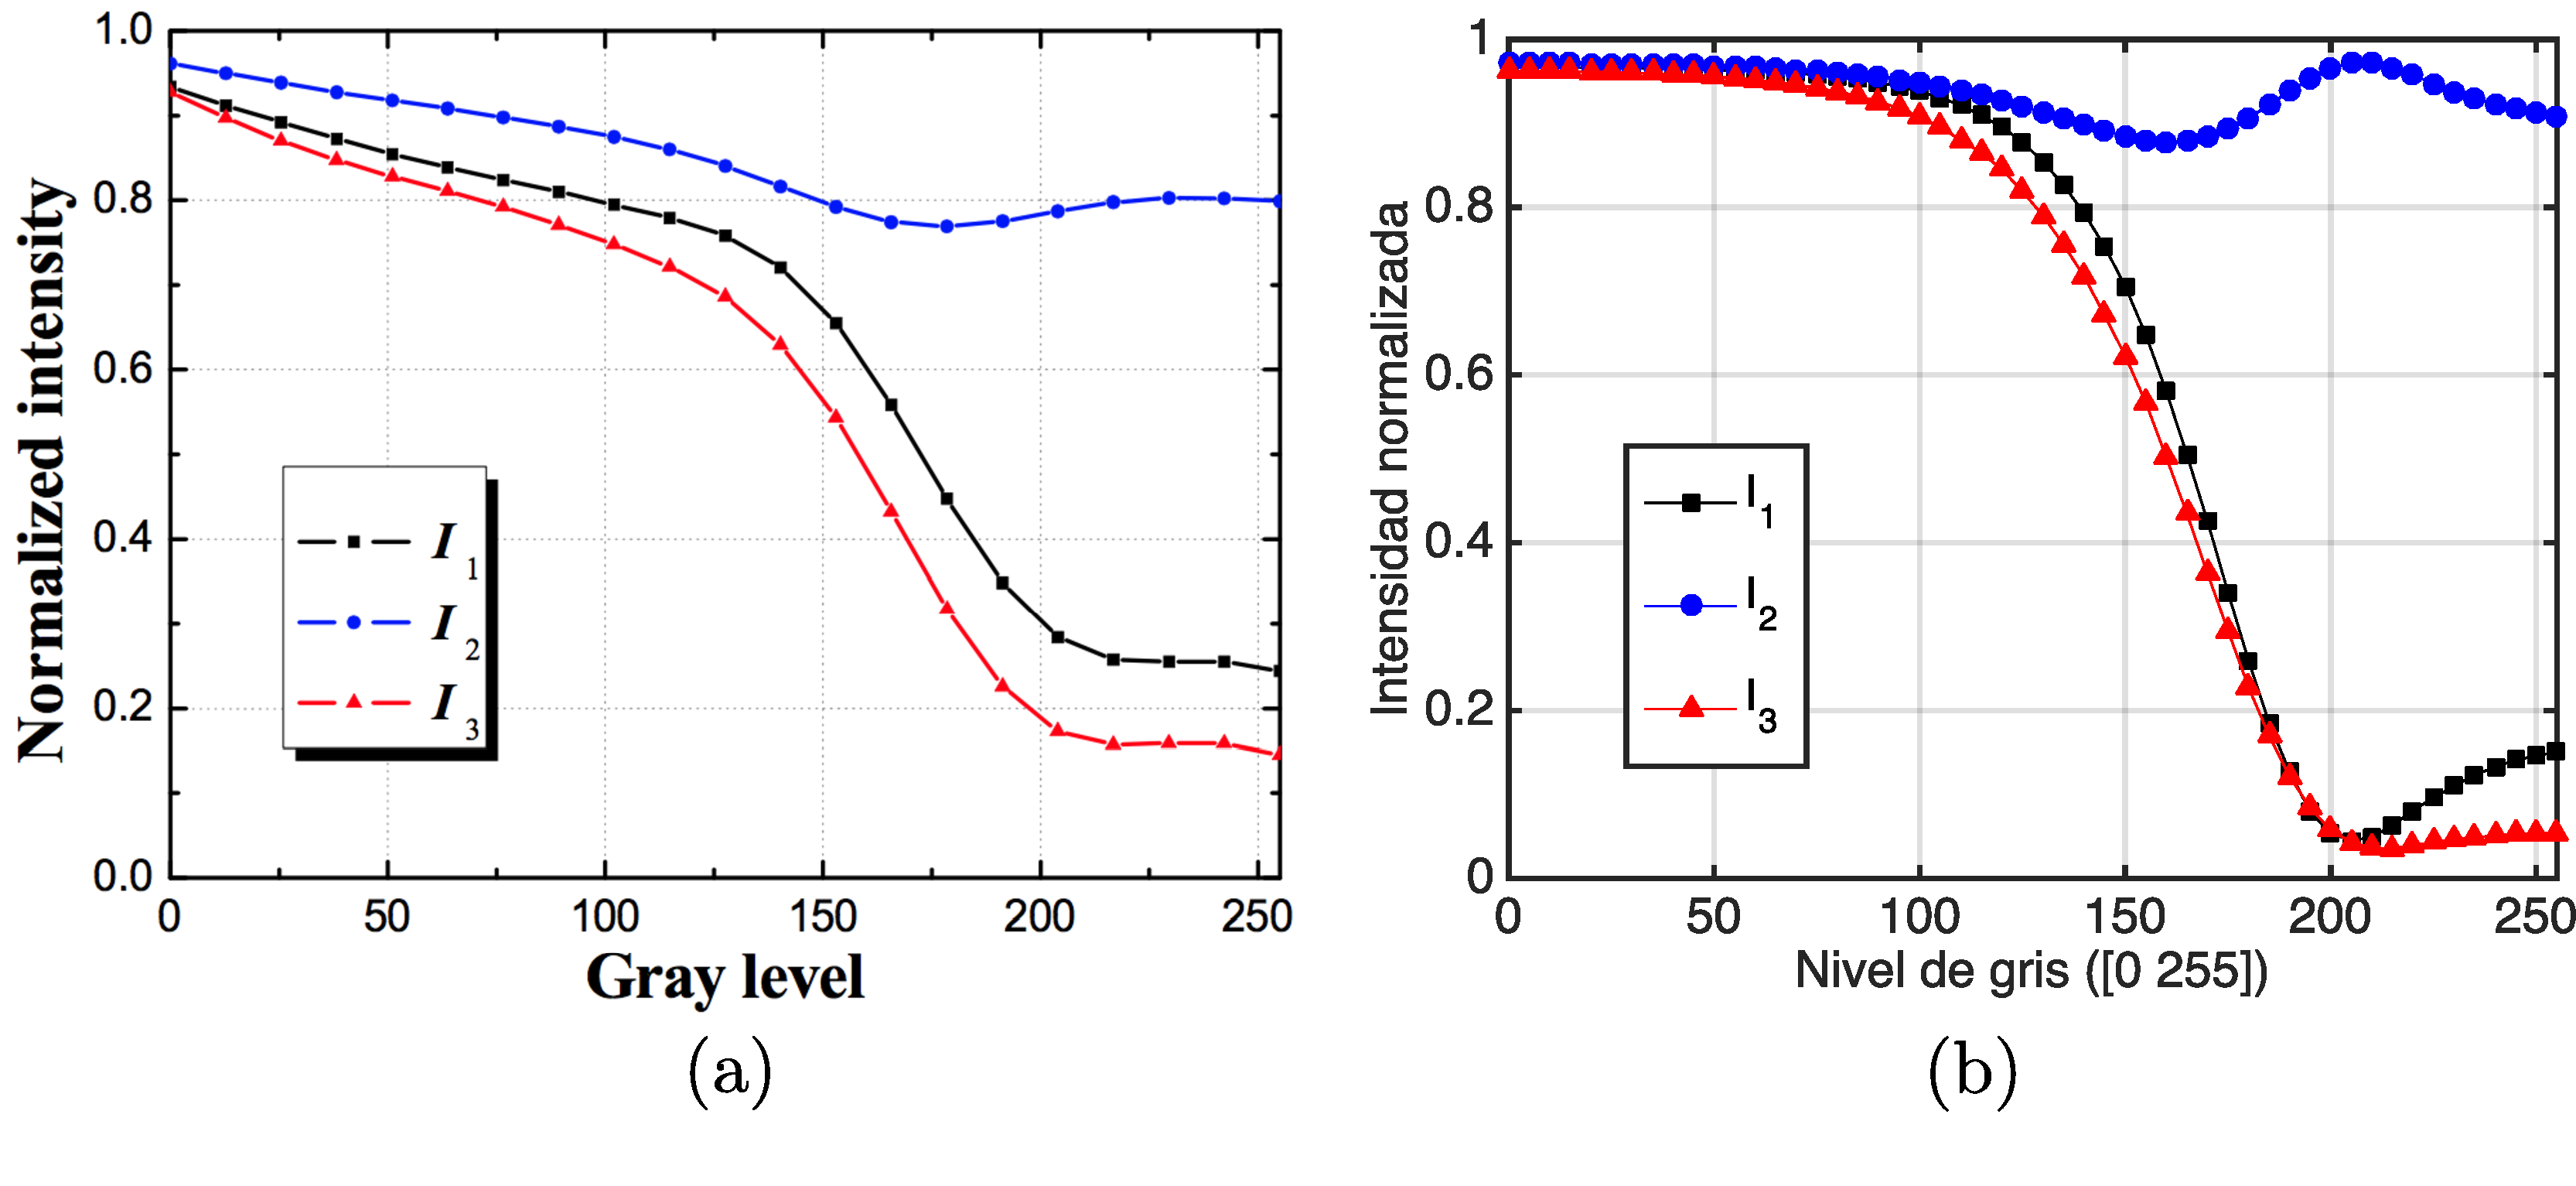
\includegraphics[scale = .27]{Ma_and_our_Is.pdf}
\caption[Comparación entre las tres intensidades para calibración
medidas por Ma et al.~ para un SLM similar y por
nosotros.]{Comparación entre las tres intensidades para calibración 
medidas por \citetChGen{Ma2014}~ (a) y por nosotros (b).}
\label{fig:Ma_and_our_Is}
\end{figure}
Asimismo, calculamos los valores de los cuadrados de los parámetros de
Jones siguiendo las ecuaciones mencionadas y obtuvimos los resultados
presentados en la Fig. \ref{fig:Our_Ma_X2Y2Z2W2}. 
\begin{figure}[h!]
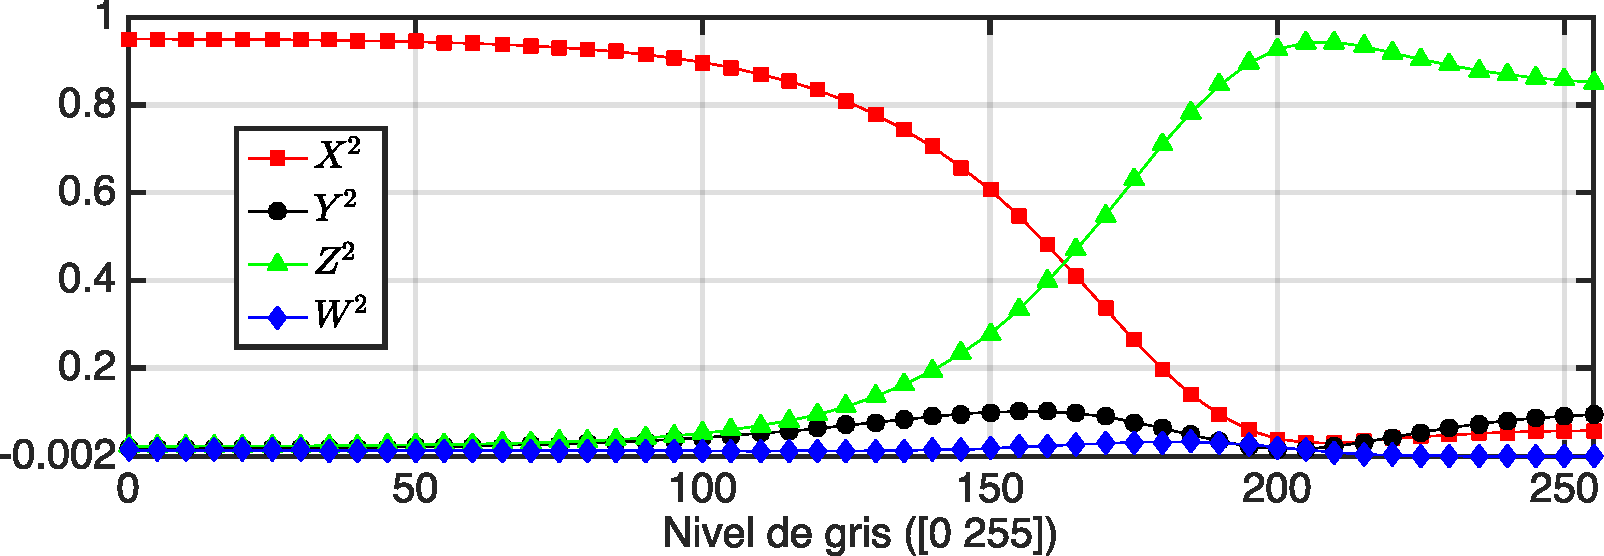
\includegraphics[scale = .55]{Our_Ma_X2Y2Z2W2_long.pdf}
\caption[Valores de $X^2$, $Y^2$ $Z^2$ y $W^2$ encontrados por
nosotros utilizando el método de Ma et al.]{Valores de $X^2$, $Y^2$ $Z^2$ y $W^2$ encontrados por
nosotros utilizando el método de Ma et al.}   
\label{fig:Our_Ma_X2Y2Z2W2}
\end{figure}
Una primera dificultad que identificamos aplicando el método de Ma fue
la ausencia de un mecanismo para definir el signo de la raíz
cuadrada de $X^2$, $Y^2$, $Z^2$ y $W^2$. Por otra parte, observamos
que aproximadamente a partir del nivel 200 la curva de $Y^2$ cambia de
direcci'on sugiriendo un cambio de signo en $Y$ y aparecen valores negativos
en la curva del parámetro $W^2$. Lo segundo produce raíces complejas no
permitidas por la teoría, y puede ser debido a variaciones leves
en la intensidad registrada por la cámara. La presencia de
valores negativos no es discutida en los artículos consultados y no
hemos identificado una restricción teórica que impida observar este
fenomeno al hacer las restas de las intensidades. Con el fin de
obtener un resultado similar al de \citetChGen{Ma2014} asumimos
  que $Z$ y $W$ son negativos y calculamos el parámetro $W$ como
  $W=\sqrt{|W^2|}$ para evitar valores complejos. Nuestros
  resultados se comparan con los de Ma et al en la Fig. \ref{fig:Ma_and_our_XYZW}.
\begin{figure}[h!]
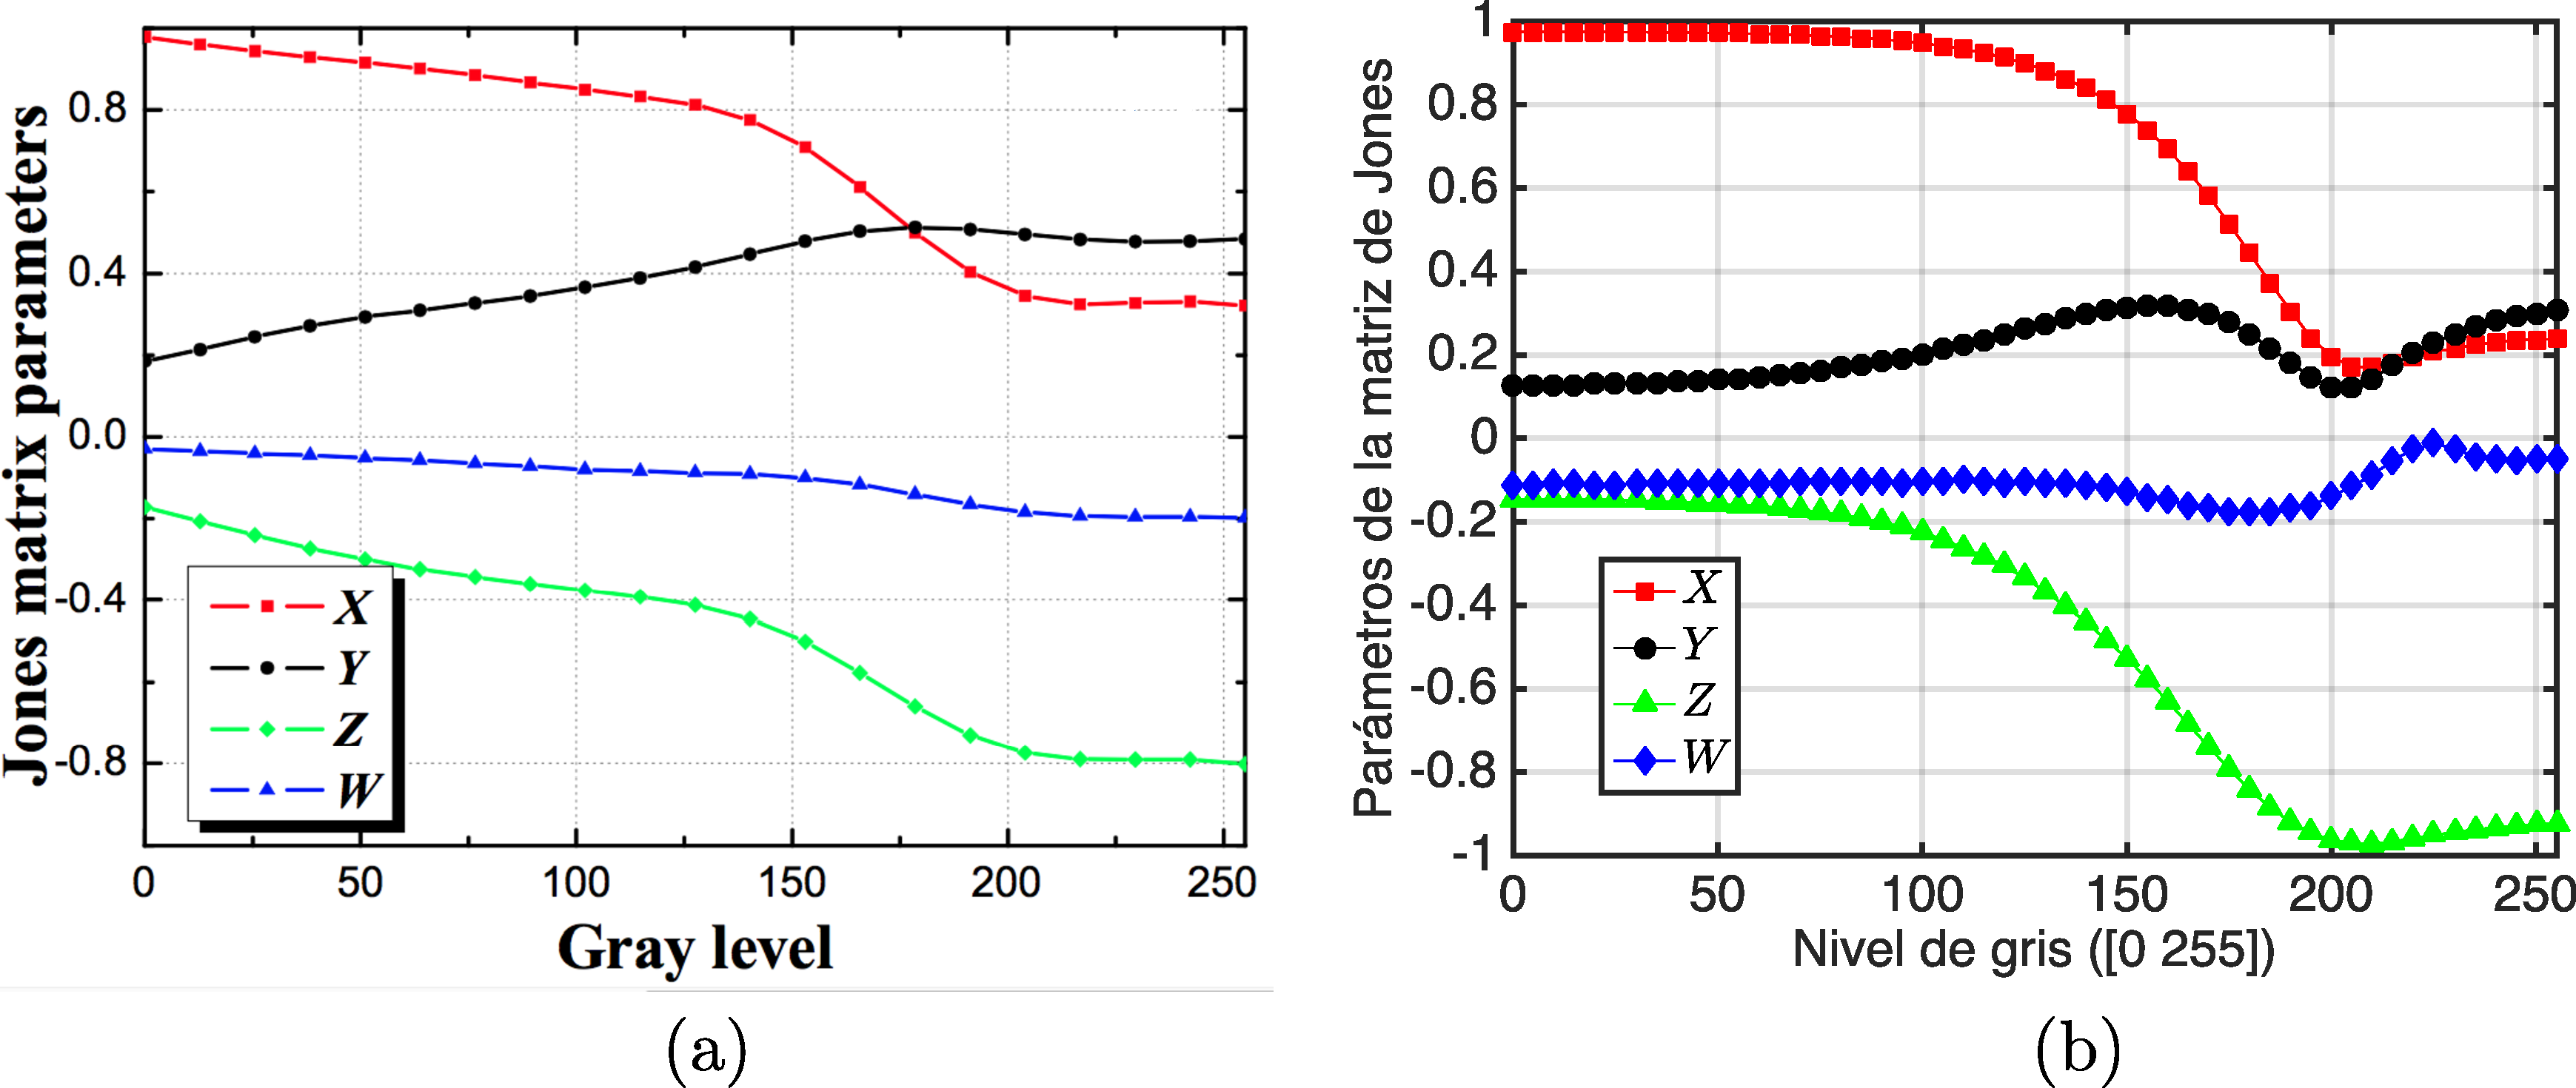
\includegraphics[scale = .26]{Ma_and_our_XYZW.pdf}
\caption[Comparación entre los valores de $X$, $Y$ $Z$ y $W$ encontrados por
Ma et al.~ para un SLM similar y por nosotros.]{Comparación entre los
  valores de X, Y Z y W encontrados por \citetChGen{Ma2014}~ 
  (a) y por nosotros (b). Dado que no queda explícito cómo encontrar
  el signo de los parámetros en ninguna de sus publicaciones, asumimos
  que $Z$ y $W$ son negativos como ellos lo presentan.}   
\label{fig:Ma_and_our_XYZW}
\end{figure}
En primera medida, en la Fig. \ref{fig:Ma_and_our_XYZW} se observa que
las curvas de los parámetros $X$, y 
$Y$ siguen la misma tendencia descendente que la encontrada por
\citetChGen{Moreno2003}, dónde la matriz comienza siendo muy similar a
una matriz identidad con $X$ cercano a uno y el resto de parámetros
tendientes a cero. Por otra parte, y también de acuerdo con otros
autores \citepChGen{Saleh1990,Marquez2000} se observan valores de $W$
cercanos a cero y valores de $Y$ 
que aumentan proporcionalmente al nivel de gris. El hecho de que $W$
sea muy cercano a cero es consistente con el modelo basado en los
parámetros físicos del modulador de
\citetChGen{Marquez2000} y con la
Eq. \ref{eq:TN-LCD_Jones_Matrix} derivada en la sección
\ref{sec:Propiedades_opticas_de_TNLCD} de este documento. 

\subsection{Comprobación experimental con 100 medidas}
\label{sec:exp_validation}
Hemos comparado las intensidades predichas por las matrices obtenidas
y encontramos que el modelo emula con muy buena exactitud tanto las 3 medidas
de entrada como las 3 medidas ortogonales. Para cada uno de los 6
estados el error absoluto promedio es menor a $2\times10^{-4}$.  Se
calcula el error absoluto promedio para cada estado como,
\begin{equation*}
error_i = \sum_{n=1}^{52}\frac{|I_n^e-I_n^s|}{52}.
\end{equation*}   
No obstante, observamos que la predicción del modelo no tiene una
exactitud igual de buena para estados distintos a los estados usados
para la caracterización. 
Con el fin de comprobar que las matrices obtenidas eran un modelo adecuado
del SLM se hicieron 100 medidas nuevas de modulación de amplitud y se
compararon con las simuladas. En esas medidas se hicieron todas las combinaciones
posibles entre 10 vectores Ket y Bra usando la 
numeración que se esquematiza en la Fig. \ref{fig:braket_100_notation}.
\begin{figure}[h!]
\centering
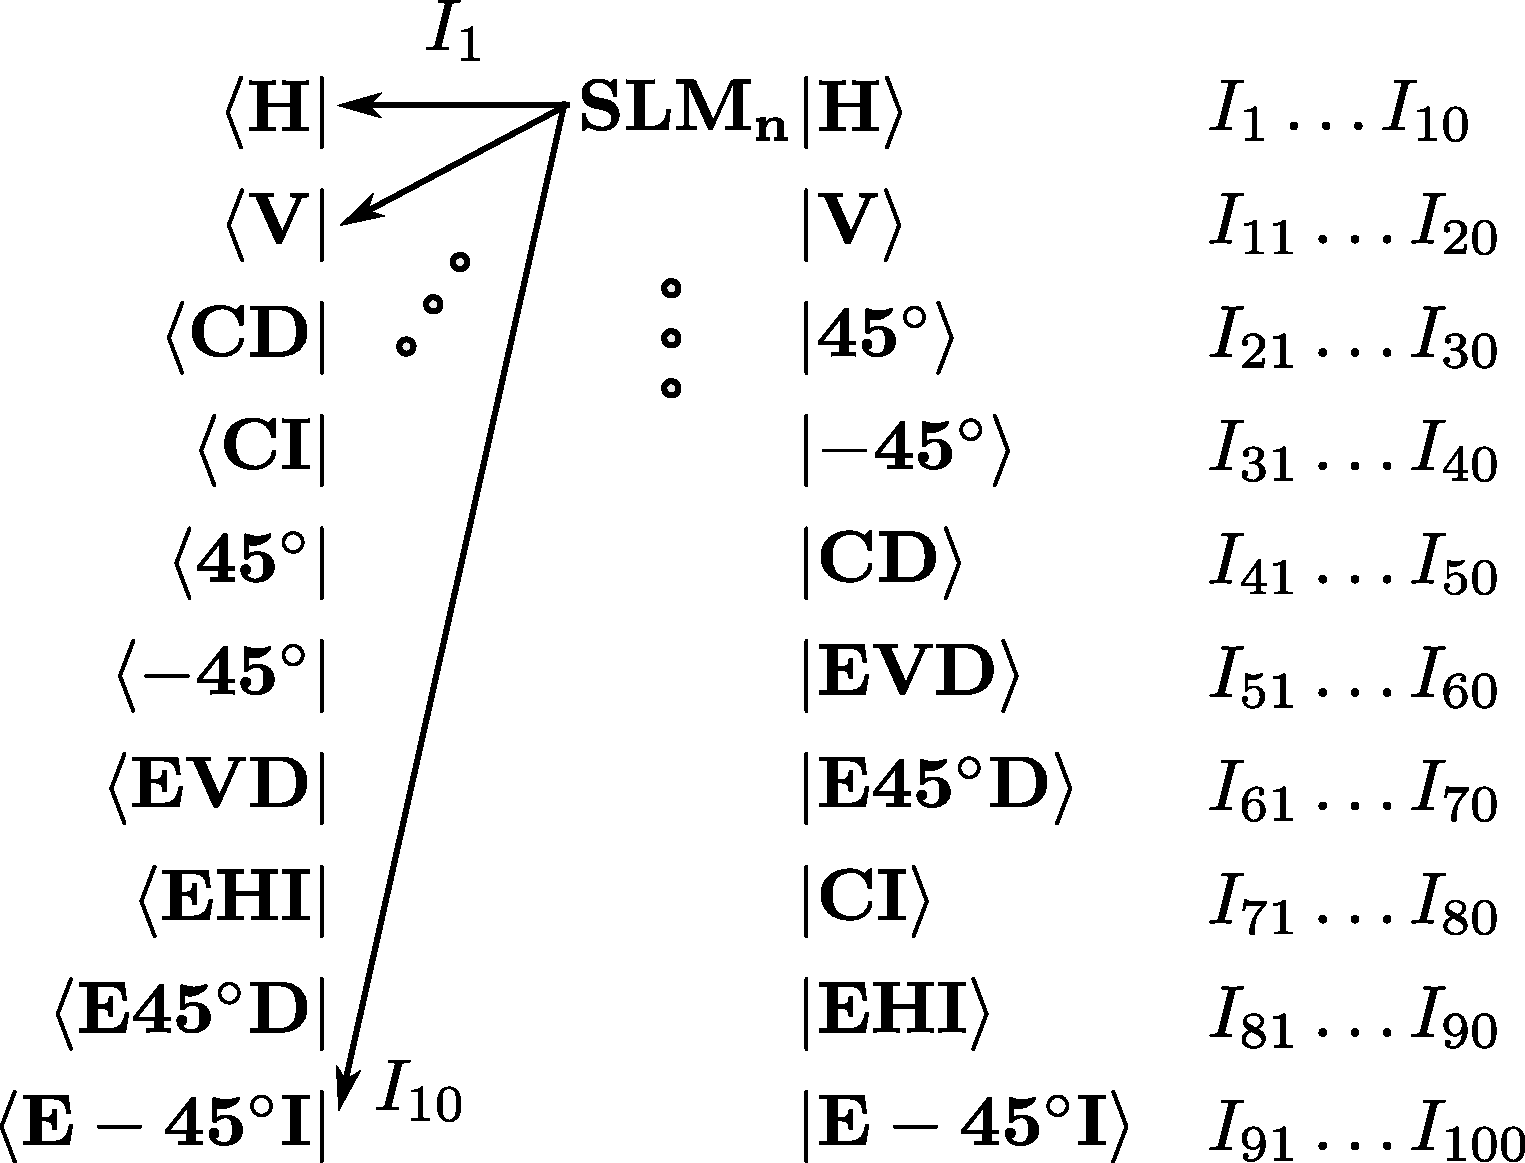
\includegraphics[scale=.4]{brakets.pdf}
\caption[Numeración de medidas experimentales de modulación para
corroboración del modelo de SLM]{Numeración de medidas experimentales de modulación para
corroboración del modelo del SLM. Por cada Ket hay 10 Bra y la
numeración se hace entre parejas en orden descendente con los pares
representados en la figura. }
\label{fig:braket_100_notation}
\end{figure}
Entre los estados se incluyeron dos parejas de estados
elípticos ortonormales no usados
como entrada del algoritmo de minimización. Los estados elípticos
corresponden a polarizaciones elípticas horizontal, vertical, a
$45^{\circ}$ y a $-45^{\circ}$ con ángulo de elipticidad $\theta
=22.5^{\circ}$ como se muestra en la Fig. \ref{fig:elliptic_states}.
\\
Para saber cómo ubicar los
elementos ópticos que generan y detectan estados de polarización
elípticos arbitrarios usamos un software desarrollado y registrado por nosotros en el Grupo de
Óptica Aplicada y presentado como una ponencia de póster en el evento
\href{http://www.eafit.edu.co/focuslatinoamerica2014/Paginas/Inicio.aspx}{\textbf{FOCUS
    Latinoamérica}} en Noviembre del 2014. El póster junto con la
interfaz gráfica y las librerías pueden ser descargadas sin costo en
el siguiente vínculo web:\\
\hspace*{\fill}
\href{https://github.com/bebopsan/Ellipsometry\_for\_dummies.git}{\textbf{https://github.com/bebopsan/Ellipsometry\_for\_dummies.git}}\hspace*{\fill}.\\

Aún cuando la imprecisión del método se hace evidente de forma
cualitativa, se midió un error promedio global para los
100 estados como medida cuantitativa, $$error_g =
\sum_{i=1}^{100}\frac{error_i}{100},$$ y se obtuvo un valor de $error_g
= 0.085628$. Es decir que con intensidades normalizadas la diferencia
entre la medida y la simulación es de alrededor de $8\%$.
Cuatro de los 100 resultados que incluyen estados elípticos se muestran en la
Fig. \ref{fig:Ma_caracterization_results} y el resto de medidas se han
puesto al alcance del lector como un notebook de iPython en un
repositorio alojado también en GitHub en el enlace: \href{http://goo.gl/69kSu2}{\textbf{http://goo.gl/69kSu2}}. 
Ese vínculo dirige a una copia del archivo que
usamos para cargar y calcular los parámetros de las matrices de Jones
del SLM usando el método de Ma et al.~ Allí se incluye tanto el código
de nuestra implementación como las figuras de los resultados. 
\begin{figure}[h!]
\centering
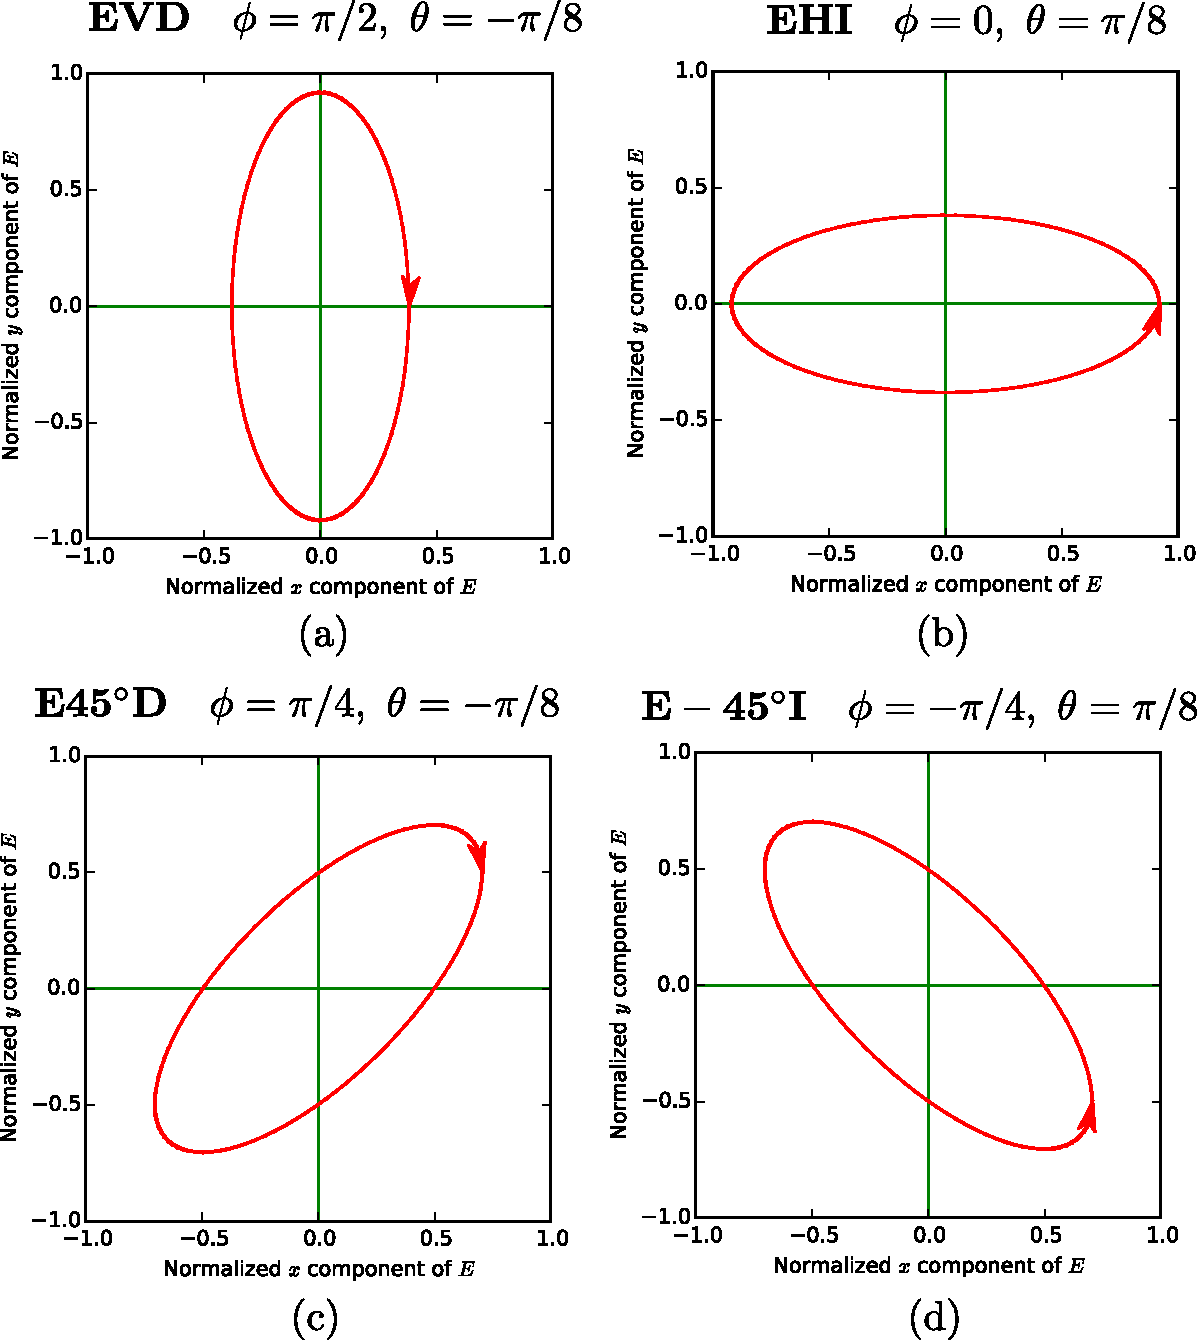
\includegraphics[scale = .6]{EVD_EHI_E45D_Em45I.pdf}
\caption[Estados de polarización elípticos]{Dos pares de estados de polarización
  elípticos ortonormales con ángulo de elipticidad $\theta = 22.5^{\circ}$. (a) Polarización Elíptica Vertical Derecha,
  (b) Elíptica Horizontal Izquierda, (c) Elíptica a $45^{\circ}$
  Derecha, y (d) Elíptica a $-45^{\circ}$ Izquierda.}
\label{fig:elliptic_states}
\end{figure}
%\newpage
\begin{figure}[h!]
\centering
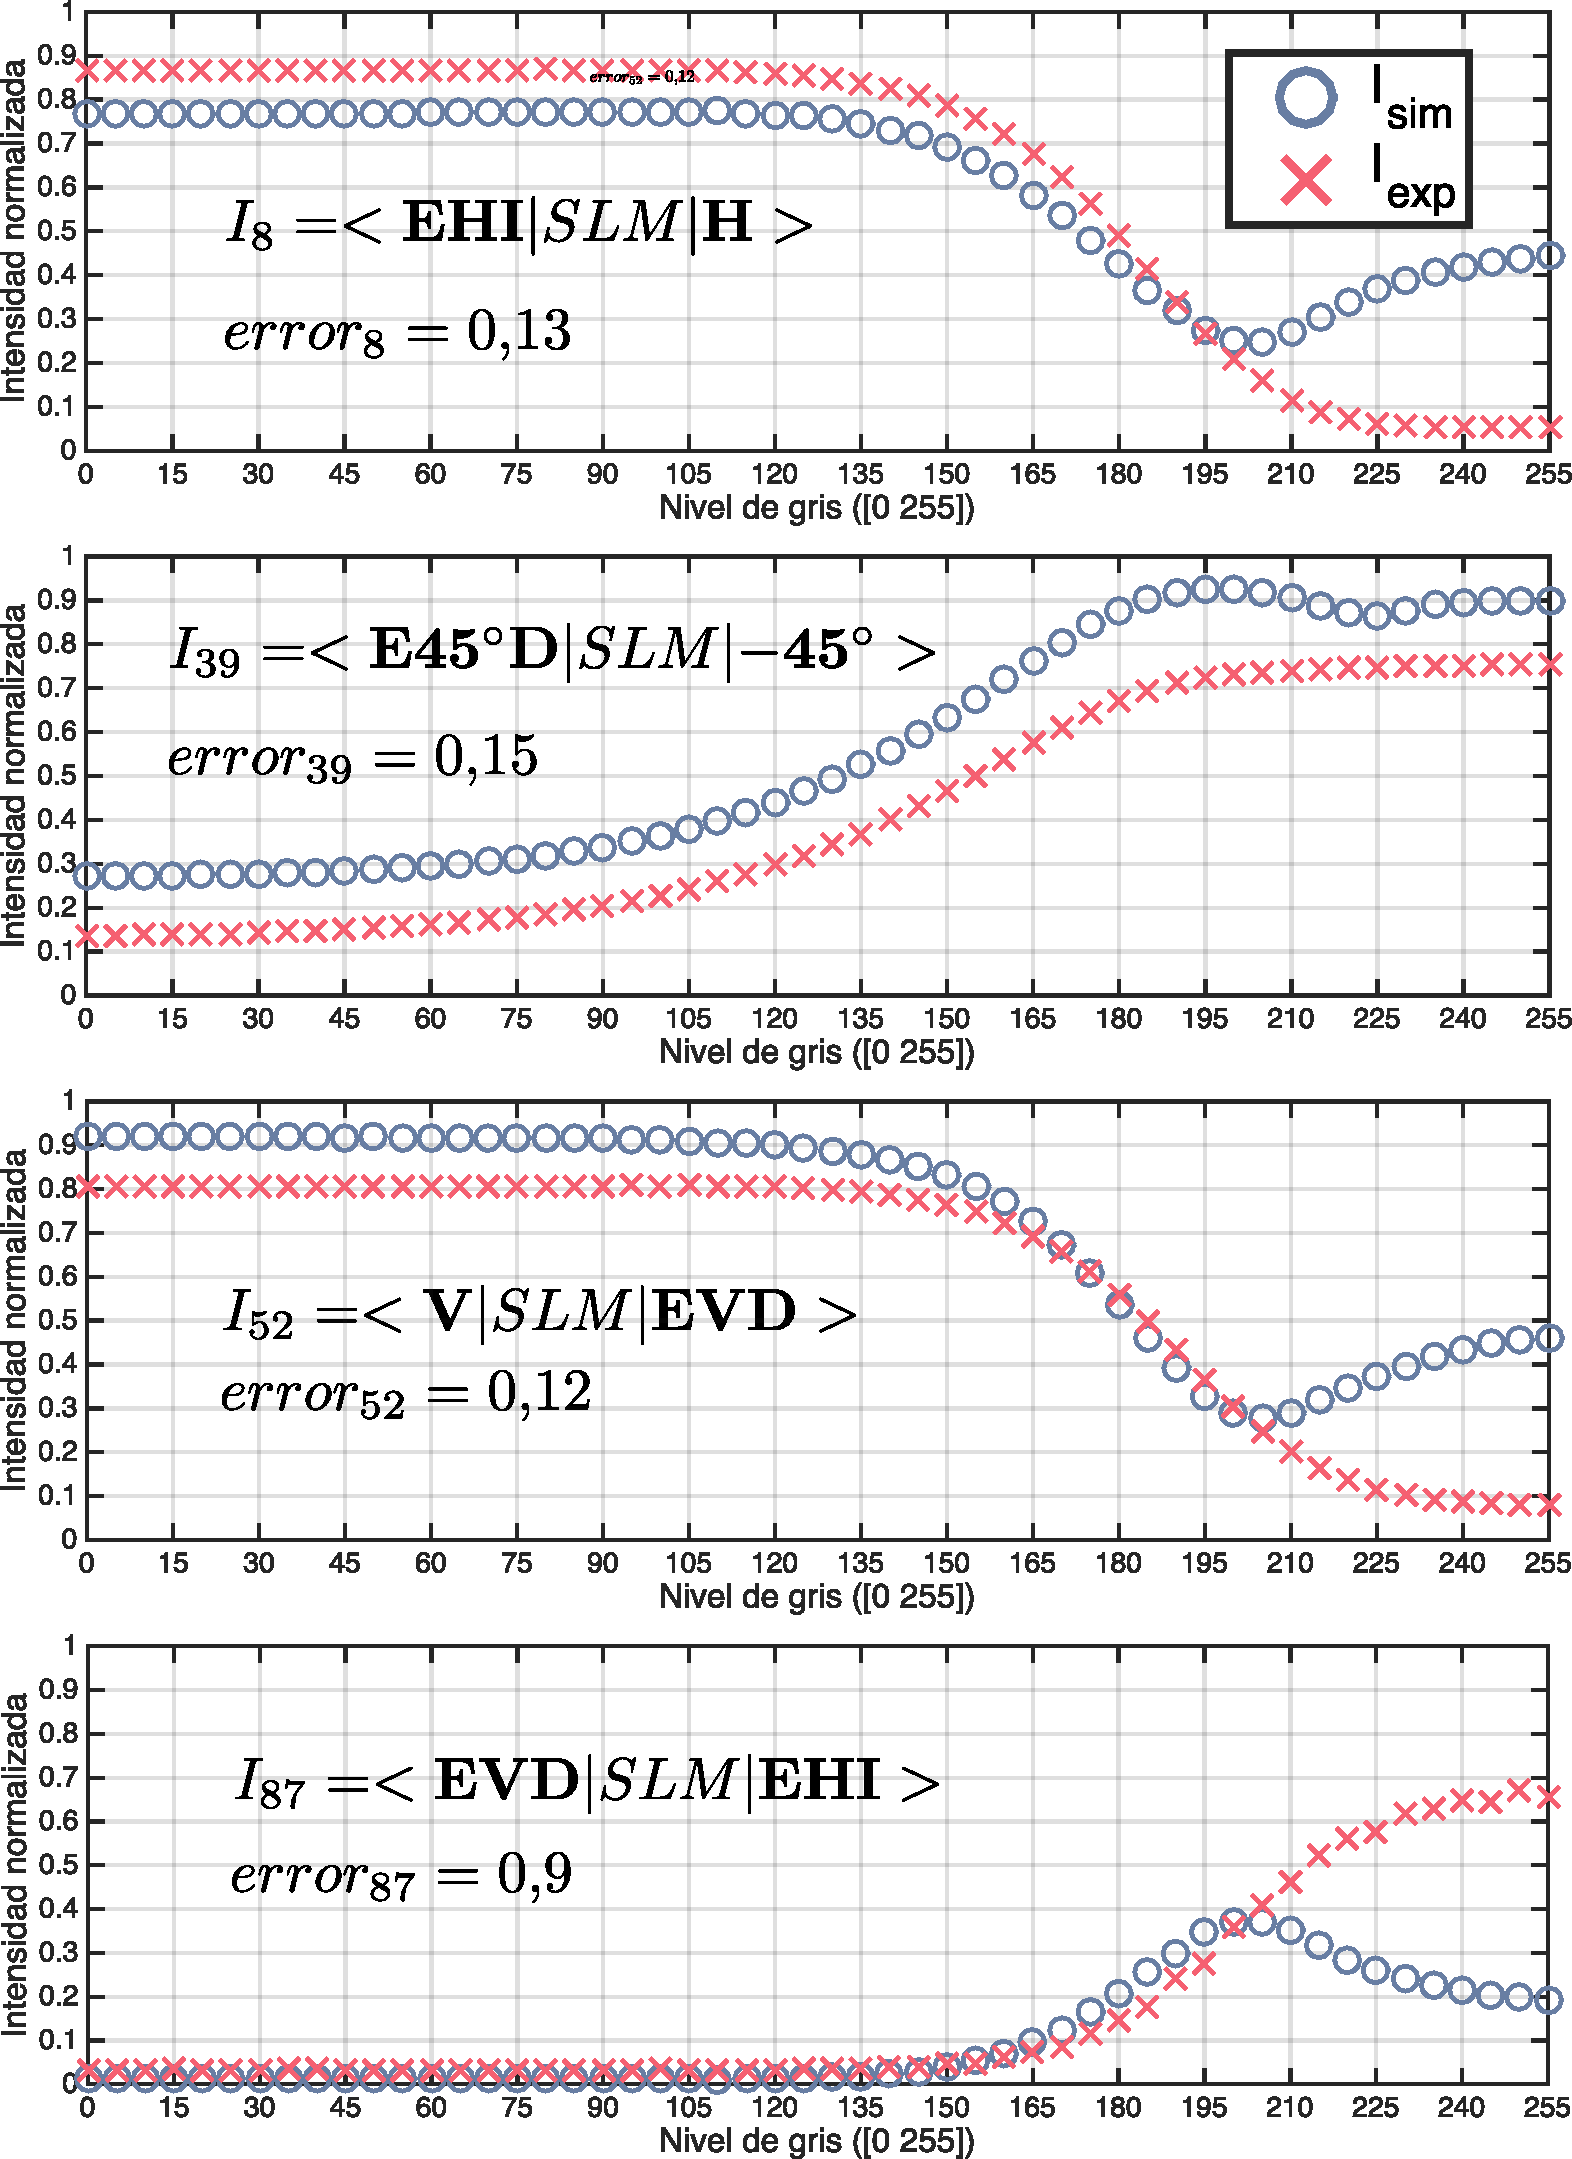
\includegraphics[scale=.5]{some_Ma_caracterization_results.pdf}
\caption[Curvas de modulación experimentales comparadas con las
simuladas usando el modelo obtenido con el método de Ma et al]{Curvas de modulación
  experimentales de 4 de las 100 medidas comparadas con sus
  equivalentes simuladas usando la matriz recuperada con el método de Ma et al.}
\label{fig:Ma_caracterization_results}
\end{figure}
Los resultados de la Fig. \ref{fig:Ma_caracterization_results} hacen
evidente que el método de Ma et al falla en reproducir el comportamiento del SLM
para algunos estados. Más aún, si se revisan las 100 medidas se observa que el
método sólo acierta a reproducir la modulación de los 12 estados $
[1,2,11,12,25,26,35,35,43,44,73,74]$ que están estrechamente ligados a
los estados usados para la construcción de las matrices. Observamos
que la divergencia del método se hace muy notoria a partir del nivel
de gris 200 y esto puede estar relacionado con el cambio de pendiente
que sufre la curva del parámetro $Y^2$ en la
Fig. \ref{fig:Our_Ma_X2Y2Z2W2} que posiblemente se debe a un cambio de
signo de $Y$. Creemos que este error está asociado con la
falta de un criterio para la selección de signos y que en vez de
adivinar signos hasta tener un modelo adecuado conviene proponer un
método de caracterización que no dependa explicitamente de $X^2$, $Y^2$, $Z^2$ y $W^2$.

% Con el fin de obtener un modelo más preciso, y que solucionara los
% vacíos del que hemos presentado, propusimos un método de
% caracterización basado en búsquedas numéricas de parámetros basándonos
% en rutinas de minimización. 

\section{Un método basado en minimización de parámetros}
Encontrar los números complejos $A$ y $B$ (o reales $X$, $Y$, $Z$,
$W$) necesarios para ensamblar la
matriz de Jones puede ser interpretado como un problema de
minimización desde el punto de vista de ingeniería inversa. Desde esta
perspectiva, se puede tratar el SLM realmente como una caja negra y
conservar sólo la condición de unicidad de la matriz
como restricción de la minimización.  
En primera medida, usamos el mismo conjunto de 6 medidas 
% polarimetría que requiere de
% plantear un conjunto de medidas que den la información suficiente
% sobre los cambios en polarización introducidos por el SLM. 
del método de caracterización 
% basados en un modelos de caja negra 
de \citetChGen{Ma2010}, que son también los estados de polarización
degenerados (lineales
$\mathbf{H}$, $\mathbf{V}$, $\mathbf{\pm 45^{\circ}}$ y circulares), que según la
teoría de polarización de Jones y de Stokes brindan la información suficiente para
caracterizar los cambios de polarización introducidos por un elemento
óptico \citepChGen{Collett2005}.
% Basandonos en el trabajo de Moreno, y con la convicción de que
% parametrizaban una variedad suficientemente diversa de situaciones
% escogimos las siguientes configuraciones de PSG y PSD para alimentar
% el algorítmo de ajuste.  
% \begin{align*}
% I_1 &= <\mathbf{V}|SLM|\mathbf{V}>& I_5 &=
%                                           <\mathbf{45^{\circ}}|SLM|\mathbf{45^{\circ}}>&I_9
%   &= <\mathbf{R}|SLM|\mathbf{R}>\\
% I_2 &= <\mathbf{H}|SLM|\mathbf{V}>&I_6 &=
%                                          <\mathbf{-45^{\circ}}|SLM|\mathbf{45^{\circ}}>&I_{10}
%   &= <\mathbf{L}|SLM|\mathbf{R}>\\
% I_3 &= <\mathbf{V}|SLM|\mathbf{H}>&I_7 &= <\mathbf{45^{\circ}}|SLM|\mathbf{-45^{\circ}}>&I_{11} &= <\mathbf{R}|SLM|\mathbf{L}>\\
% I_4 &= <\mathbf{H}|SLM|\mathbf{H}>&I_8 &=
%                                          <\mathbf{-45^{\circ}}|SLM|\mathbf{45^{\circ}}>&I_{12}
%   &= <\mathbf{L}|SLM|\mathbf{L}> 
% \end{align*}
% \begin{align*}
% I_1 &= |<\mathbf{V}|SLM|\mathbf{V}>|^2,& I_3 &=
%                                           |<\mathbf{45^{\circ}}|SLM|\mathbf{45^{\circ}}>|^2,&I_5
%   &= |<\mathbf{CD}|SLM|\mathbf{CD}>|^2,\\
% I_2 &= |<\mathbf{H}|SLM|\mathbf{V}>|^2,&I_4 &=
%                                          |<\mathbf{-45^{\circ}}|SLM|\mathbf{45^{\circ}}>|^2,&I_{6}
%   &= |<\mathbf{CI}|SLM|\mathbf{CD}>|^2.
% \end{align*}
Las curvas de modulación correspondientes a cada una de las medidas en
la notación de Ma y en notación la de la
Fig.~\ref{fig:braket_100_notation}, pueden verse en la Fig.~\ref{fig:six_input_measures}. 
\begin{figure}[h!]
\centering
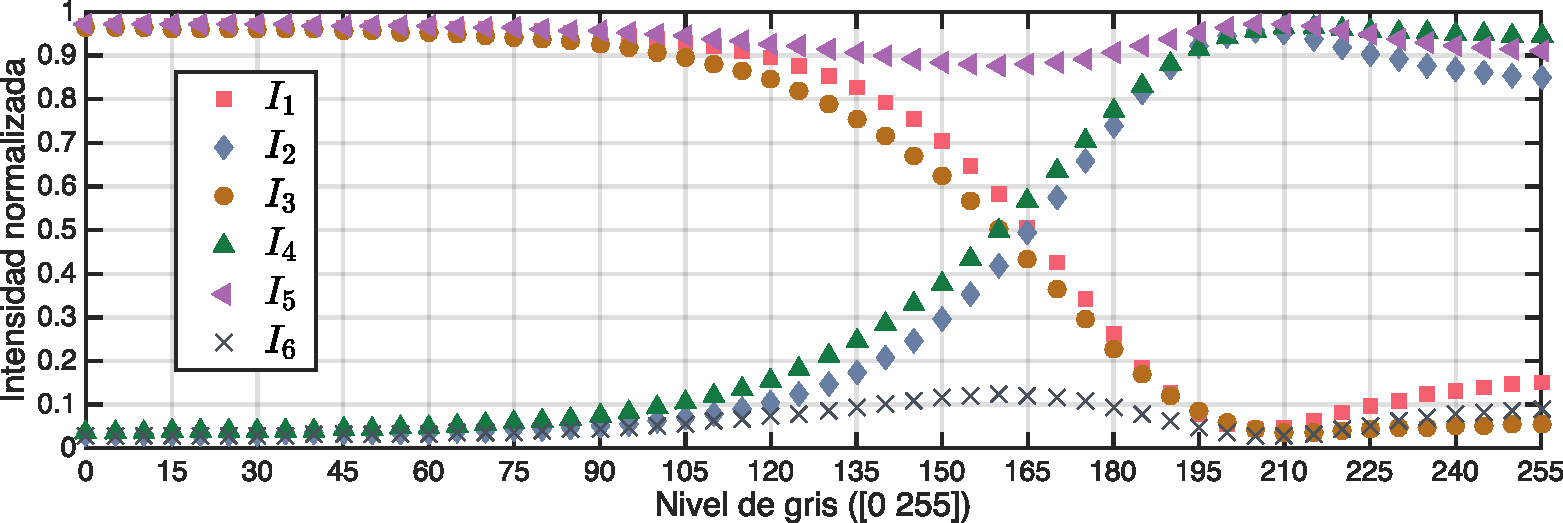
\includegraphics[scale=.55]{six_input_measures.pdf}
\caption[Curvas de modulación que sirven de entrada para el ajuste de
parámetros de la matriz de Jones del SLM]{Curvas de modulación que
  sirven de entrada para el ajuste de parámetros de la matriz de Jones
  del SLM. La leyenda indica la equivalencia entre las 6 curvas del
  método de Ma et al y la notación usada para las 100 medidas de comprobación. }
\label{fig:six_input_measures}
\end{figure}
Se puede observar que la modulación de amplitud es muy similar entre
polarizaciones lineales y que, como sería de esperarse, hay
complementariedad entre estados ortogonales.  Por otra parte, se
observa claramente que el SLM es cercano a ser transparente en un
amplio rango de niveles cuando se genera y detecta polarización
circular derecha, y opaco cuando se genera polarización circular
derecha y se detecta circular izquierda.
A continuación se describe la el funcional usado para la función de
minimización y la implementación del método. 
\subsection{Funcional a minimizar}
Una matriz de Jones que represente correctamente al SLM, encontrada por
métodos de minimización, debería en principio poder
emular al menos estas 6 medidas para lograr resultados tan buenos como
los del método de Ma et al. Nosotros planteamos un funcional a
minimizar ($\mathcal{L}$) que actúa como una medida de la similitud entre 
intensidades simuladas e intensidades adquiridas experimentalmente. El
funcional sirve como un criterio de selección para evaluar si los
parámetros propuestos ($(\mathbf{X,Y,Z,W})$) en alguna de las iteraciones de la rutina de
minimización son parámetros que reproduzcan las medidas
experimentales.  
\begin{equation}
\mathcal{L}(\mathbf{X,Y,Z,W}) = \sum_{ng=0}^{255}\sum_{i=1}^6 | I_{ng,i} -
|<\mathbf{J_{i}}|\mathbf{SLM_{ng}}|\mathbf{J_{i}}>|^2|^2.
\label{eq:ChGen_SLM_model_functional}  
\end{equation}
El funcional de la Eq. \ref{eq:ChGen_SLM_model_functional}  consiste en
la suma de las diferencias cuadradas entre intensidades para cada
nivel de gris ($n$) y para cada combinación de PSG y PSD ($i$). Los
argumentos del funcional son vectores que representan el conjunto de números
reales $X_n, Y_n, Z_n, W_n$ que componen a los elementos complejos $A$ y $B$
de la matriz de Jones del SLM (ver 
Eq. \ref{eq:general_jones_matrix}) para un $n$ dado,
\begin{align*}
\mathbf{X} &= \sum_{n=0}^{255}X_n,&\mathbf{Y} &= \sum_{n=0}^{255}Y_n,&\mathbf{Z} &= \sum_{n=0}^{255}Z_n,&\mathbf{W} &= \sum_{n=0}^{255}W_n.
\end{align*} 
El funcional \ref{eq:ChGen_SLM_model_functional}  puede ser minimizado
variando los 1024 ($256\times 4$) posibles valores 
de $X,Y,Z,W$ dentro del rango $-1:1$ en un algoritmo de
minimización. La minimización de los datos presentados en la
Fig. \ref{fig:six_input_measures} se llevo a cabo usando la función,\\
\hspace*{\fill}
\href{http://goo.gl/tv5Iyz}{\bf{scipy.optimize.fmin\_l\_bfgs\_b}}, \hspace*{\fill}\\ del
 paquete de calculo científico \href{http://goo.gl/fRhz8s}{\textbf{Scipy}} del
 lenguaje de programación \href{https://www.python.org}{\textbf{Python}}. Ésta
 función conocida como \href{http://en.wikipedia.org/wiki/Limited-memory\_BFGS}{\textbf{L-BFGS-B}} implementa una versión de memoria limitada del método quasi
 Newton conocido como Broyden-Fletcher-Goldfarb-Shano y permite
 la definición de condiciones de frontera sobre los argumentos de
 entrada.  
La implementación en el lenguaje Python de la función a minimizar se
muestra en la Fig. \ref{fig:SLM_functional},  
\begin{figure}
\begin{python}
def min_sq(x0,I_exp):
    """ Calculates squared differences for a minimization procedure.

    Given the experimental meassures of intensity and arbitrary values for 
    the parameters of an SLM Jones Matrix, this function gives a value to
    minimize. That value tells how close is the estimation of x, y, z, w 
    to the value that correctly models the SLM.

    :param x,y,z,w: Are a guess of real scalars that conform the Joung Matrix for the SLM.
    :param I_exp: Is a dictionary contanining intensities for every polarization state.
    """
    # brakets is a dictionary containing each pair of Jones vectors
    brakets = {1:translate_Ellipse_to_Jones([ 0,   0],      [0,0]),\
           2:translate_Ellipse_to_Jones([ pi/2,0],      [0,0]),\
           3:translate_Ellipse_to_Jones([ pi/4, 0],    [pi/4,0]),\
           4:translate_Ellipse_to_Jones([-pi/4, 0],    [pi/4,0]),\
           5:translate_Ellipse_to_Jones([pi/4,-pi/4],   [pi/4,-pi/4]),\
           6:translate_Ellipse_to_Jones([ -pi/4,pi/4],  [pi/4,-pi/4])}
    [x,y,z,w] = x0
    M = matrix([[ x + y*1j, z + w*1j],\
                [-z + w*1j, x - y*1j]])
    min_sum = 0
    I_sim = {}
    for i in range(1,nMeasures):
        Out, In = brakets[i]
        I_sim[i] = (In.H*M.H*Out * Out.H*M*In)
        min_sum += ((I_sim[i]-I_exp[i])**2)[0,0].real    
    return min_sum
\end{python}
\caption{Funcional a minimizar para el ajuste de parámetros basado en
  6 medidas de modulación de amplitud.}
\label{fig:SLM_functional}
\end{figure}
%\pagebreak
y la llamada a la función de minimización se hace como se muestra en la
Fig. \ref{fig:SLM_minimization}.
%cons = ({'type': 'eq', 'fun': lambda x:  x[0]**2+x[1]**2+x[2]**2+x[3]**2 - 1})
\begin{figure}
\begin{python}
bnds = ((-1, 1), (-1, 1),(-1, 1), (-1, 1))
x,y,z,w = [0.0001, 0.0001, -0.0001, -0.0001] 
res_f = {}
for g in range(52):
    I_exp = I_list[g]
    res = fmin_l_bfgs_b(min_sq, [ x,y,z,w], fprime = None,\
                         approx_grad = 1,args = (I_exp,brakets),\
                         pgtol=1e-05, bounds =bnds)
    x,y,z,w = res[0]
    res_f[g] = res[0]
    print(res[0])
\end{python}
\caption{Condiciones de frontera, argumentos iniciales y llamado de la
función de minimización (fmin\_l\_bfgs\_b) para cada nivel de gris.}
\label{fig:SLM_minimization}
\end{figure}
En este caso usamos un valor semilla para los valores de entrada muy
cercano a cero, utilizamos la opción de aproximación del gradiente
por medio de diferencias finitas y definimos la tolerancia de
convergencia como criterio de parada cuando el valor del funcional no
cambie menos de $1e^{-5}$. Los detalles sobre las variables,
preprocesamiento, y los resultados se han subido a internét en un
repositorio de GitHub y se pueden observar en la siguiente página
web:\\
\hspace*{\fill} \href{http://goo.gl/FLIGE0}{\textbf{http://goo.gl/FLIGE0}}.\hspace*{\fill} \\
%\hspace*{\fill} \href{http://goo.gl/QQtcQX}{\textbf{http://goo.gl/QQtcQX}}.\hspace*{\fill} \\
En la figura \ref{fig:xyzw} se presentan los valores de $X,Y,Z,W$ obtenidos luego de
ejecutar la minimización. 
\begin{figure}[h!]
\centering
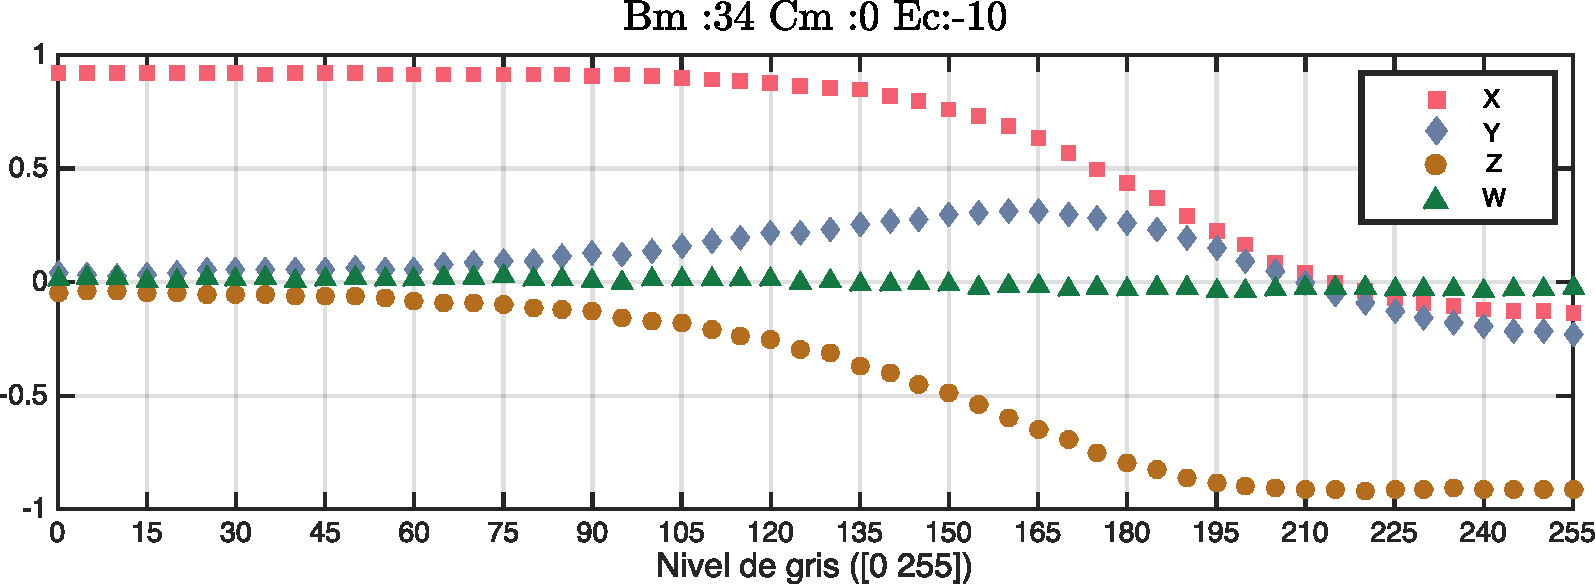
\includegraphics[scale=.55]{xyzw.pdf}
\caption[Parametros reales que conforman la matriz de Jones del SLM
encontrados por minimización con 6 medidas]{Parametros reales que
  conforman la matriz de Jones del SLM encontrados por medio de
  minimización con 100 entradas.} 
\label{fig:xyzw}
\end{figure}
Contrario a lo que pensábamos, resultó que aún cuando el método de
minimización se basa directamente en los valores $X,Y,Z$, y $W$, y no
en sus cuadrados, los resultados son casi idénticos a los que
obtuvimos en la sección anterior con el método de Ma et~al. Las curvas
de los parámetros del modulador siguen la misma tendencia y producen
los mismos valores de intensidad en las simulaciones. Las 4 medidas
con estados elípticos que se  
presentaron en la Fig. \ref{fig:Ma_caracterization_results} se
repitieron para el nuevo método y se presentan junto con el valor del
error relativo promedio porcentual en la
Fig. \ref{fig:6m_caracterization_results}. 
%\newpage
\begin{figure}[h!]
\centering
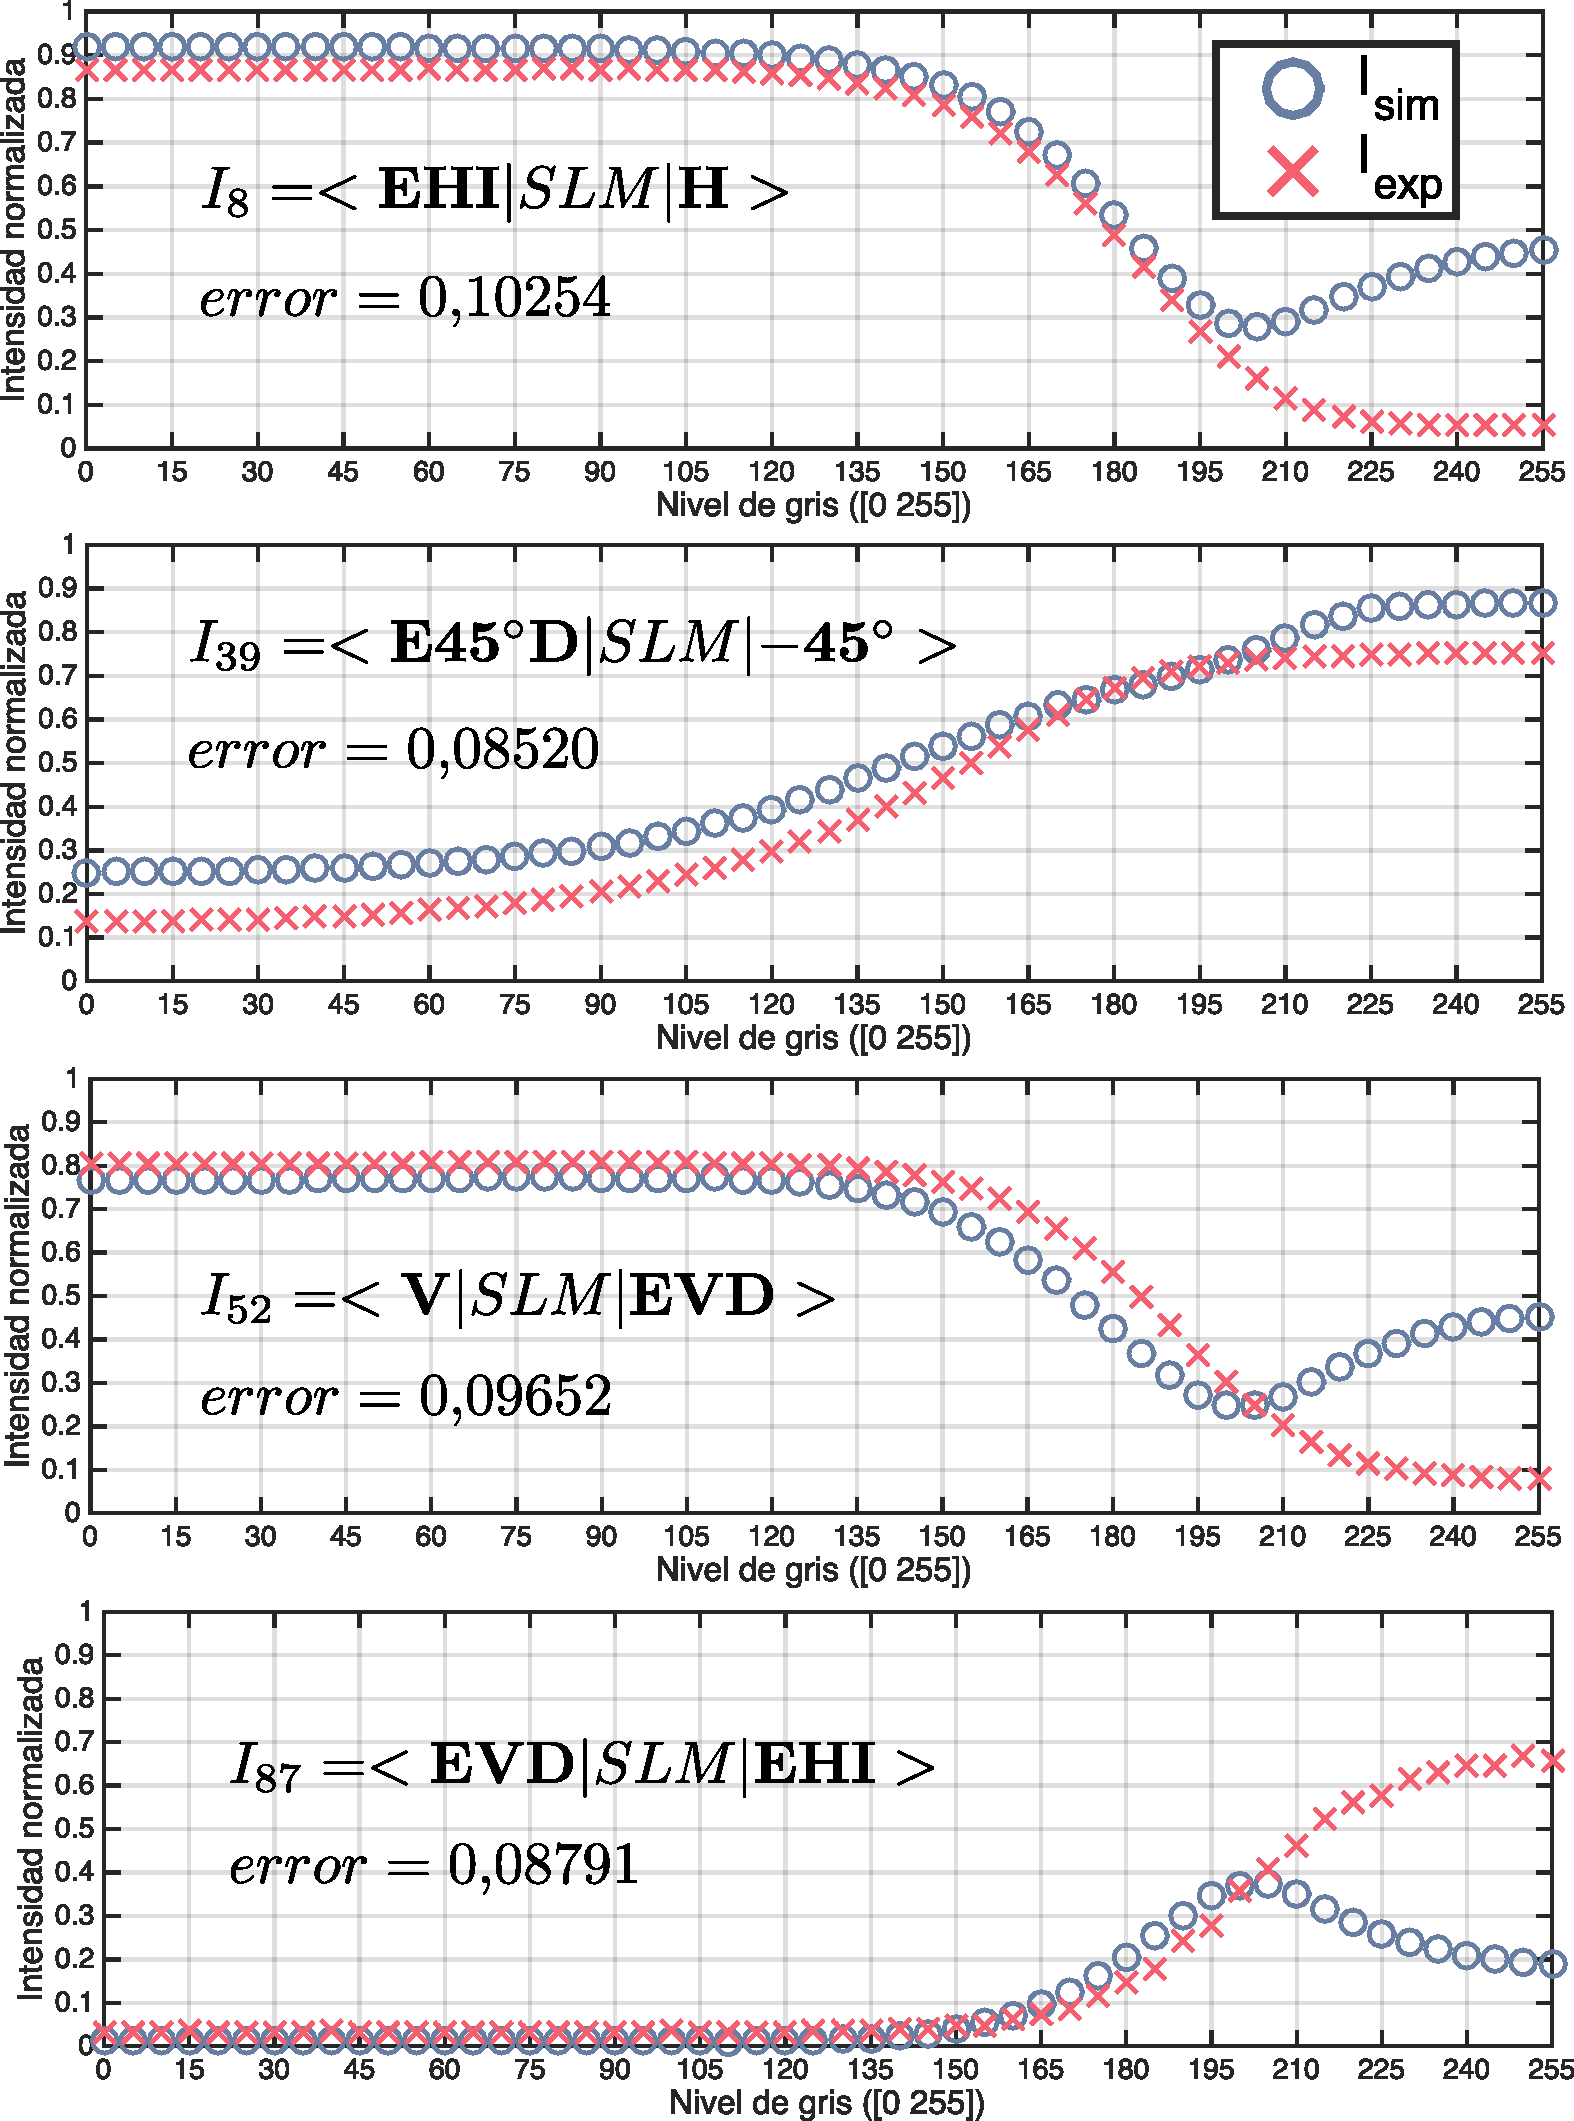
\includegraphics[scale=.5]{some_6min_caracterization_results.pdf}
\caption[Curvas de modulación experimentales comparadas con las
simuladas usando el modelo obtenido con el método de minimización de 6
medidas]{Curvas de modulación
  experimentales, y error de 4 de las 100 medidas comparadas con sus
  equivalentes simuladas usando la matriz recuperada con el método de
  minimización con 6 medidas.}
\label{fig:6m_caracterization_results}
\end{figure}
El error en las 6 medidas usadas como entrada es en este caso menor a
$2\times10^{-4}$, y el error absoluto global es de $error_g
=0.077673$, que es un poco menor que el anterior. Sin embargo, sigue ocurriendo que la exactitud se pierde a partir del
nivel de gris 200 en la mayoría de los estados. Es decir, que con estas medidas como entrada
nuestro método es tan bueno como el de la literatura pero no
significativamente mejor.
\pagebreak
\subsection{Una ampliación de la función de minimización}
El funcional de minimización puede ser modificado
fácilmente para incluir como valores de entrada cuantos BraKet's
distintos se deseen siempre y cuando se conozcan los vectores de Jones 
correspondientes al PSG y PSD de cada uno.   
Siguiendo la idea de utilizar la información extra de la que disponemos, modificamos la
función para recibir no 6 sino 100 estados de entrada y 
ejecutamos de nuevo el algoritmo de minimización. Los parámetros de
Jones para cada nivel de gris del método de minimización extendido
se presentan en la Fig. \ref{fig:xyzw_100}, e inmediatamente se puede observar un
cambio importante en el comportamiento de las curvas $X$, $Y$, y $W$
en comparación con las figuras \ref{fig:Ma_and_our_XYZW} y
\ref{fig:xyzw}. 
\begin{figure}[h!]
\centering
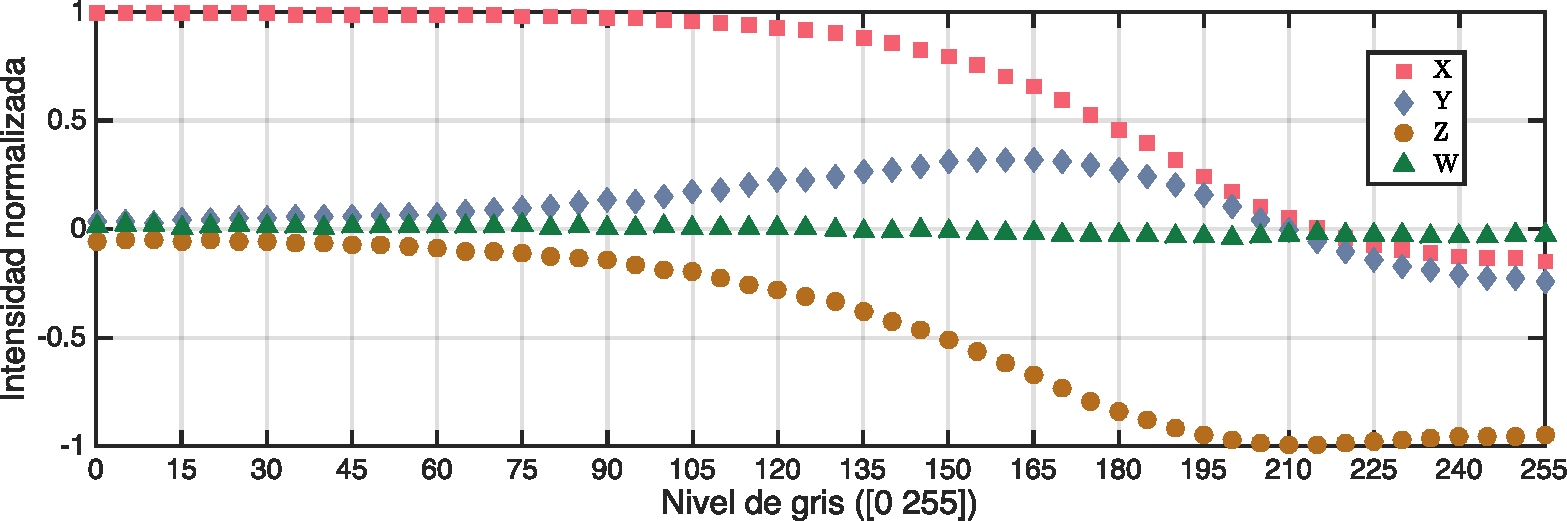
\includegraphics[scale=.55]{xyzw_100.pdf}
\caption[Parametros reales que conforman la matriz de Jones del
SLM encontrados por minimización con 100 medidas]{Parametros reales
  que conforman la matriz de Jones del SLM 
  encontrados por medio de minimización con 100 entradas.}
\label{fig:xyzw_100}
\end{figure}
Como se había supuesto, se puede ver que los valores de $Y$
para los niveles más allá del 200 son negativos, y que $W$ es
virtualente cero para todo el rango de niveles. Además, se observa que
$X$ también adquiere valores negativos para niveles de gris por encima
de 200.   
Con respecto a las medidas de intensidad, se obtuvo una mejoría cuantitativa
significativa con un error absoluto global de $error_g= 0.024162$ que
es 3.5 veces menor que el obtenido con el método de Ma et al. No
obstante, la calidad de la solución se hace más evidente cuando se
comparan los resultados cualitativamente, y se observa que los cambios
de dirección que surgían a partir del nivel de gris 200 han
desaparecido. Como antes, se presentan 4 de las medidas con estados
elípticos en la Fig. \ref{fig:100m_caracterization_results} y los
resultados completos han sido 
alojados en \href{http://goo.gl/kZjVGU}{\textbf{http://goo.gl/kZjVGU}}.
\begin{figure}[h!]
\centering
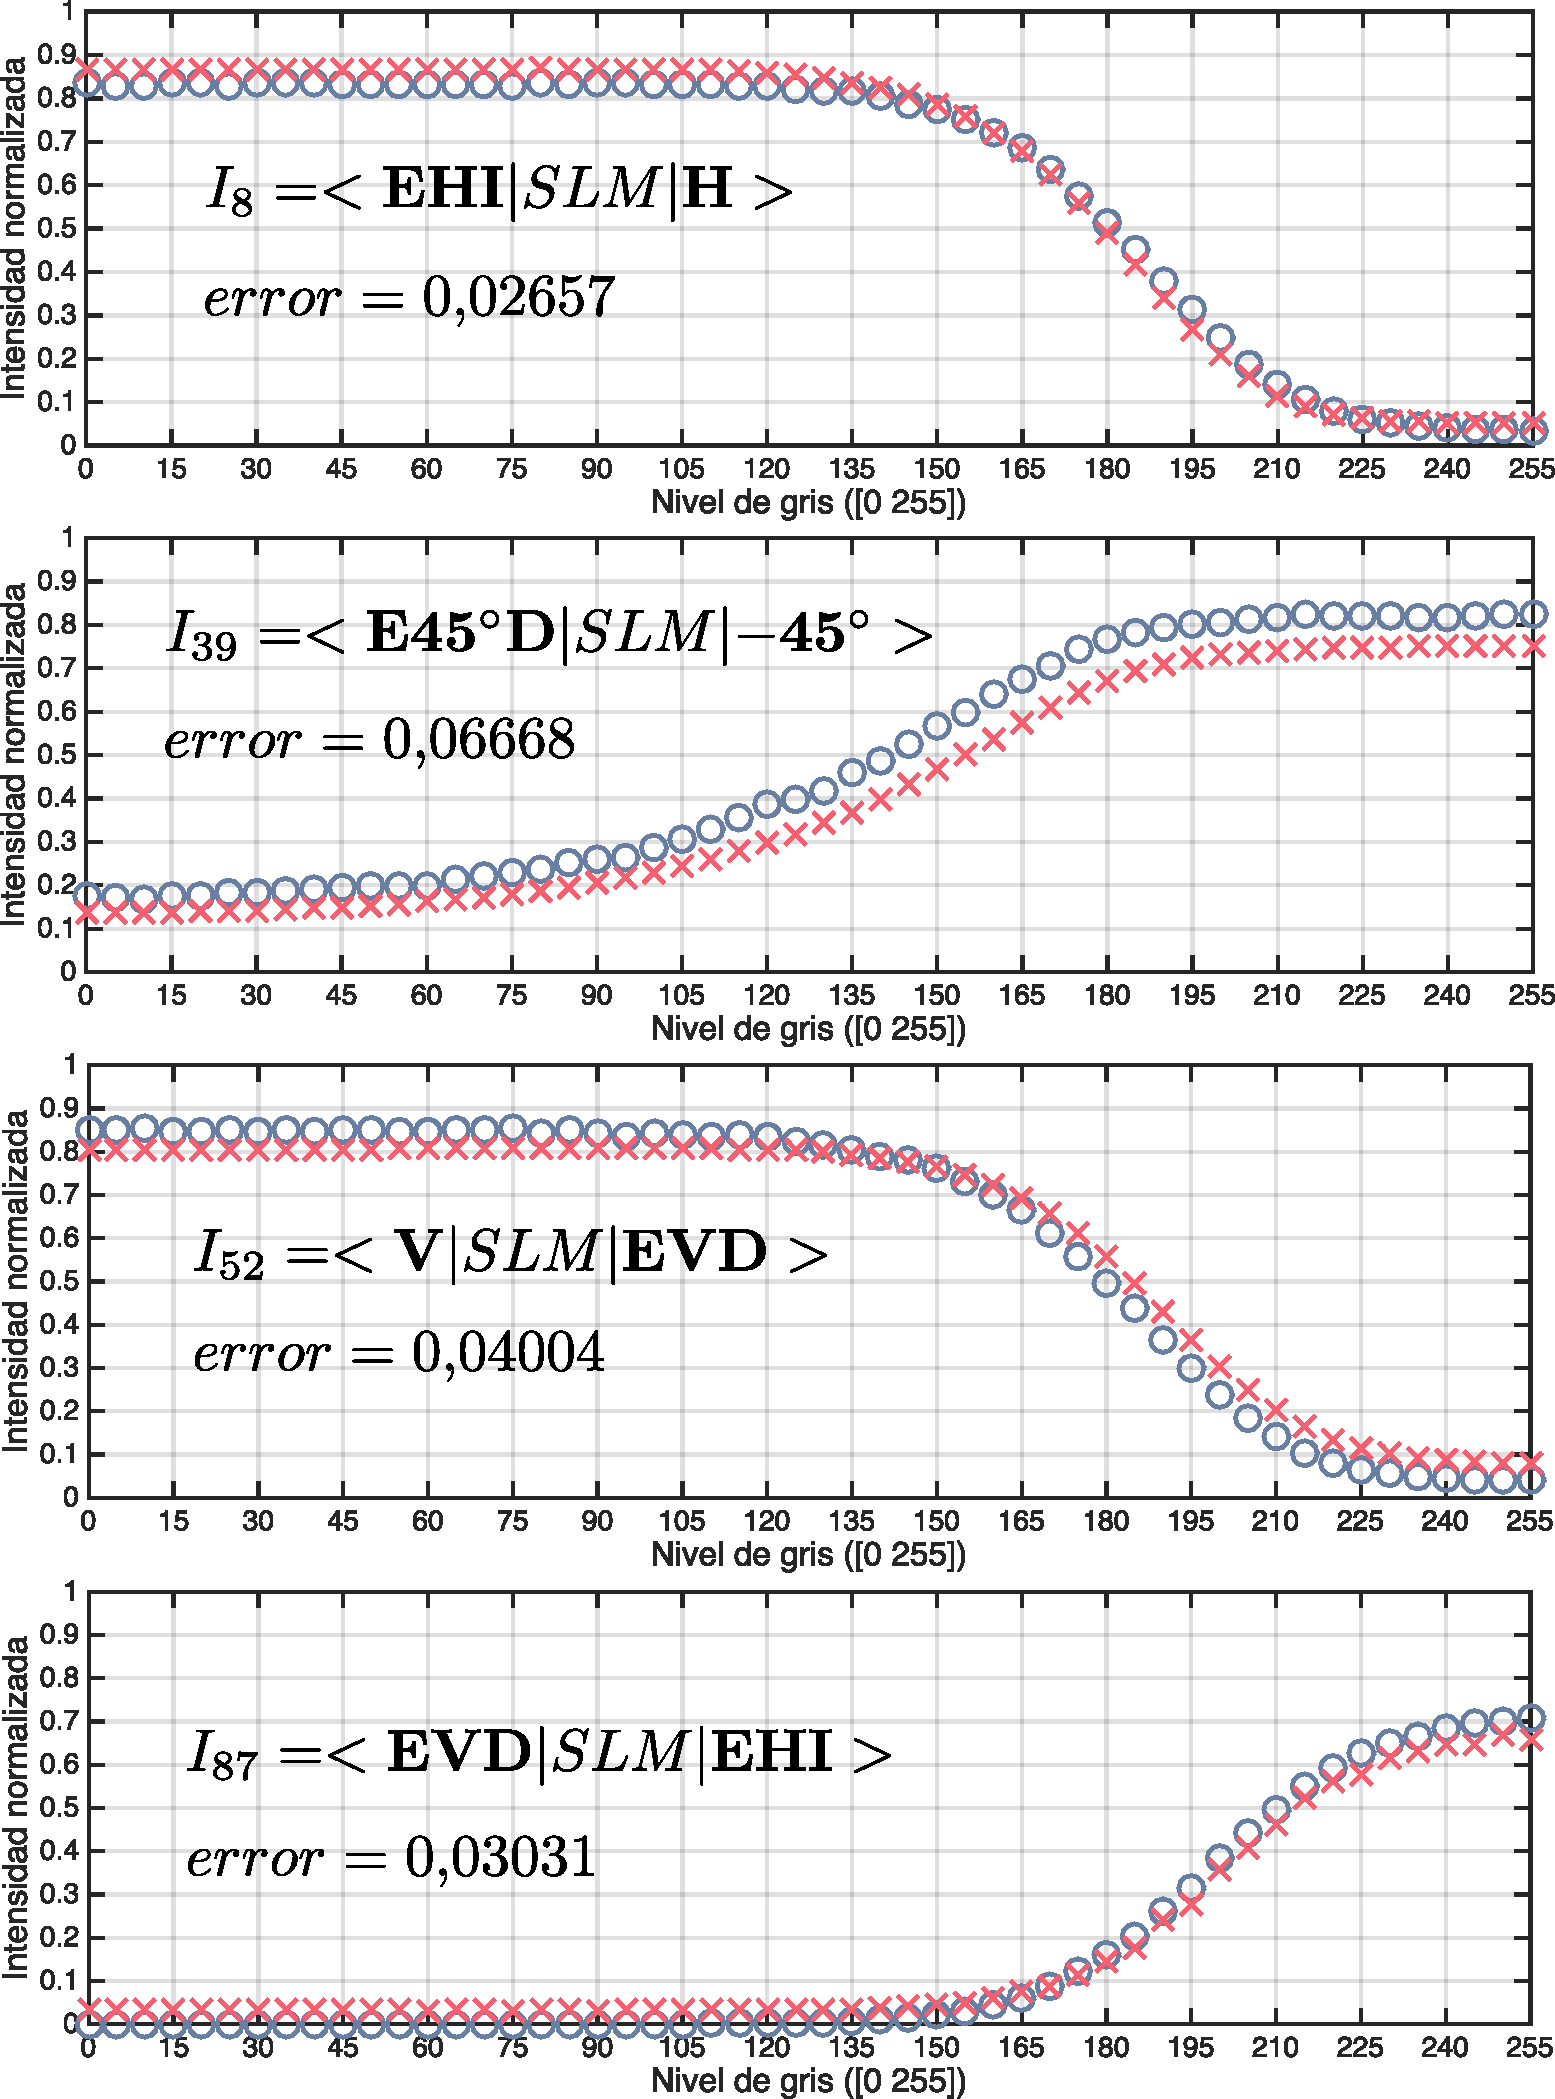
\includegraphics[scale=.5]{some_100_caracterization_results.pdf}
\caption[Curvas de modulación experimentales comparadas con las
simuladas usando el modelo obtenido con el método de minimización de 100
medidas]{Curvas de modulación
  experimentales, y error de 4 de las 100 medidas comparadas con sus
  equivalentes simuladas usando la matriz recuperada con el método de
  minimización con 100 medidas de entrada.}
\label{fig:100m_caracterization_results}
\end{figure}
En conclusión, Lo que muestran los resultados es que se logró una muy buena aproximación, y que el modelo de la matriz de Jones del SLM efectivamente
reproduce la modulación de amplitud del elemento real. 
\subsubsection{Instrumento para la automatización del proceso de
  medida.}
\label{sec:instrumento}
Ahora bien, cualquiera que haya tenido experiencia con la
caracterización de SLMs se sorprenderá por la cantidad de medidas que
hemos hecho. La toma de cientos de medidas y todo el proceso de
aprendizaje sobre la polarimetría fue posible sólo
porque usamos un instrumento mecatrónico desarrollado por nosotros
antes y durante este trabajo de grado. El Instrumento se muestra en la
Fig. \ref{fig:montaje_real_polarimetro} y consiste en
cuatro rotadores ópticos motorizados manipulados por un computador a
traves de la tarjeta de prototipado rápido
\href{http://www.arduino.cc/en/Main/ArduinoBoardLeonardo}{\bf{Arduino Leonardo}}. 
\begin{figure}[h!]
\centering
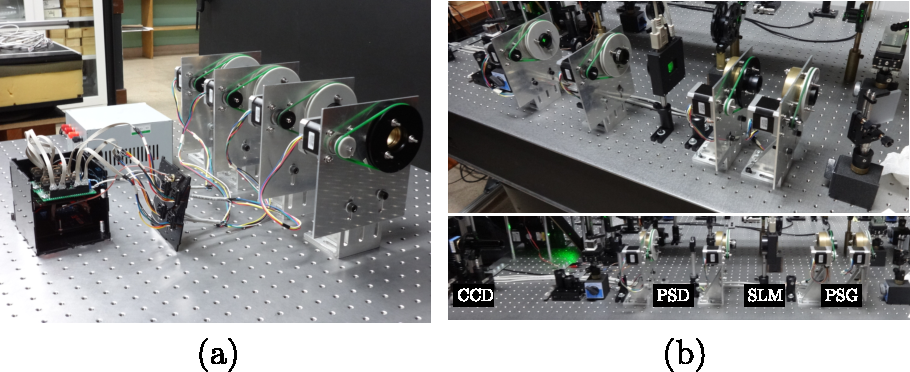
\includegraphics[scale=.96]{montaje_real_polarimetro.pdf}
\caption[Hardware del instrumento de polarimetría y montaje
experimental ]{(a) Hardware del instrumento de polarimetría que se
  compone de 4 rotadores de elementos ópticos, una fuente de voltaje,
  y una caja de circuitos electrónicos en donde está el Arduino y la
  electrónica de potencia. (b) Montaje experimental correspondiente a
  la implementación de la Fig. \ref{fig:PSG_PSD}. }
\label{fig:montaje_real_polarimetro}
\end{figure}
 La interfaz de usuario del instrumento para toma de medidas y
calibración de motores fue programada como un
instrumento virtual del entorno de programación gráfica LabView, y los
comandos de movimiento para los motores son enviados al Arduino a
través de una librería de comunicación serial implementada en Python.
Las componentes mecánicas y electrónicas del instrumento se describen a profundidad en el
apéndice \ref{AppendixA}, y los programas de interfáz de usuario y
comunicación serial se describen el apéndice B.
El proceso de toma de cientos de medidas que a una persona podría llevarle varios
días de trabajo se hace con la interfaz en cuestión de una o dos horas
sin necesidad de supervisión.    
\pagebreak
%\subsection{Medida de la modulación de fase}
\section{Medida de la modulación de fase}
% El proceso de caracterización del SLM no queda completo sin antes
% comprobar que el modelo puede predecir modulaciones de fase. 
El paso siguiente en la caracterización del SLM consiste en medir la
modulación de fase y comprobar si la matriz de Jones encontrada es
capaz de predecir el comportamiento de este SLM. 
La fase del frente de onda se midió usando el interferómetro
\href{http://en.wikipedia.org/wiki/Mach–Zehnder_interferometer}{\bf{Mach–Zehnder}}
de la Fig. \ref{fig:mach_zehnder}. 
\begin{figure}[h!]
\centering
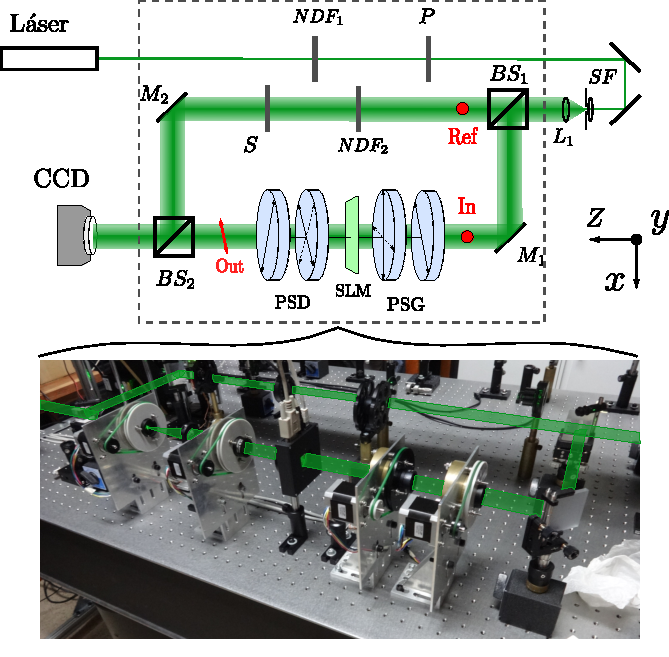
\includegraphics[scale=1.1]{mach_zehnder.pdf}
\caption[Interferómetro Mach-Zehnder para caracterización de curvas de
modulación de fase]{Interferómetro Mach-Zehnder para caracterización de curvas de
modulación de fase. }
\label{fig:mach_zehnder}
\end{figure}
En este montaje la fuente de iluminación es un láser de estado sólido
de diodo bombeado (DPSS) de longitud de onda 532nm y potencia nominal
50mW. El haz pasa por un filtro de densidad neutra ($NDF_1$) que sirve como
atenuador, y luego por un polarizador (P) de recubrimiento de
nanopartículas que garantiza una polarización lineal vertical con
relación  10.000:1. Este polarizador es usado porque el estado de
polarización a la salida del diodo láser es ligeramente elíptica y no
está perfectamente alineada con la vertical de la mesa óptica. 
Luego de ser redireccionado, el haz es filtrado, expandido y colimado
por medio de un filtro espacial (SF) en combinación con una lente
($L_1$). Una vez colimado, el haz pasa por un cubo divisor de haz no
polarizador ($BS_1$) que lo divide en un haz de referencia en la parte
superior y uno objeto en la parte inferior que ilumina
al SLM. El haz de entrada es reflejado en el espejo de primera
superficie $M_1$ y pasa a través del PSG, el SLM, y el PSD para luego
reencontrarse con el haz de referencia en un segundo cubo ($BS_2$) y
continuar su camino hasta la cámara CCD. A diferencia del haz objeto,
el haz de referencia sólo pasa por un segundo NDF que sirve para
compensar la relación entre intensidades de los dos haces. El elemento
$S$ es un obturador que se controla desde el computador y sirve para cambiar
del modo de medida de modulación de amplitud a modulación de fase.  

Al haber recorrido un camino que contiene elementos polarizadores y
birrefringentes, el haz objeto sufre cambios en su fase y en su estado
de polarización. Estos cambios se ven reflejados en la posición y
contraste de las franjas de los interferogramas registrados por la
cámara. En la figura \ref{fig:fringes} se pueden observar dos
interferogramas que se han tomado cuando a la salida del PSD hay (a)
un estado vertical, y (b) un estado horizontal.  
\begin{figure}[h!]
\centering
\includegraphics[scale=.5]{fringes.pdf}
\caption[Interferogramas obtenidos en el montaje experimental para
caracterización de modulación de fase]{Interferogramas obtenidos en el montaje experimental para
caracterización de modulación de fase. (a) Franjas de interferencia
cuando la polarización en los dos brazos es igual, y (b) cuando son
estados ortogonales.}
\label{fig:fringes}
\end{figure}

La caracterización de las curvas de modulación de amplitud está
asociada al cambio de contraste, y la modulación de fase es
proporcional al desplazamiento de las franjas. Un cambio de fase de
$\pi$ radianes hace que las franjas se desplazan hasta un punto en el
cual las que eran brillantes son ahora oscuras, y
viseversa. Caracterizar la modulación consiste en medir los 
desplazamientos de las franjas para cada nivel de gris de la pantalla
del SLM, y dado que cualquier vibración puede mover las franjas es
preferible capturar simultaneamente imágenes con las franjas en una
posición de referencia e imagenes con franjas 
desplazadas. Para ello, varios autores como \citetChGen{Moreno2003} y
\citetChGen{Ma2010} han proyectado al SLM una máscara con dos
secciones rectangulares, una con un nivel de gris constante (255) y
otra en la que el nivel de gris varía de 0 a 255. La máscara usada y
el interferograma resultante se muestran en la Fig. \ref{fig:split}.  
\begin{figure}[h!]
\centering
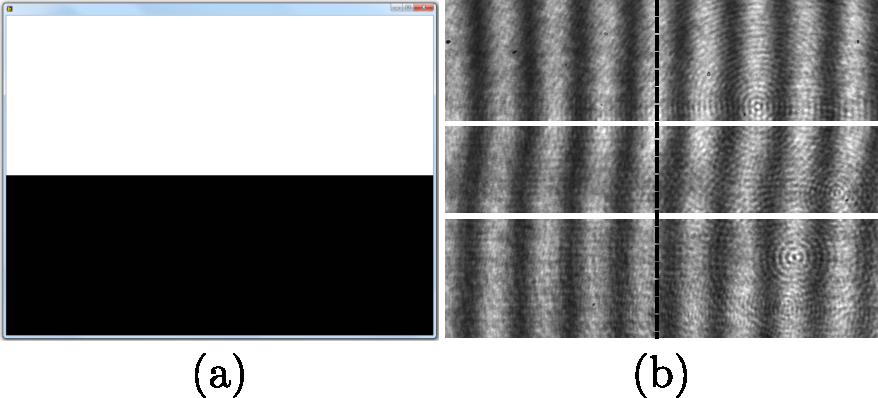
\includegraphics[scale=1]{split.pdf}
\caption[Máscara dividida e interferograma obtenido para
caracterización de modulación de fase]{(a) Máscara dividida y (b)
  interferograma registrado para
caracterización de modulación de fase. En esta combinación de PSG y
PSD se logró una modulación de aproximadamente $\pi/2$ que se puede
identificar con la línea de referencia punteada. La linea roja indica
que esa parte del interferograma se desecha.}
\label{fig:split}
\end{figure}

El interferograma de la Fig. \ref{fig:split}(b) se descompone en 3
imágenes, la imagen central se desecha, pues presenta un efecto de
borde indeseado que resulta de la difracción producida por el escalón
entre un nivel de gris y otro. Las imágenes superior e inferior corresponden a las franjas
de referencia y desplazadas respectivamente, y se conservan para
extraer la fase entre ellas. 
Para visualizar mejor las crestas
promediamos el valor de las primeras y últimas 100 filas y generamos
dos curvas en 1D de la intensidad normalizada por píxel como se
observa en la Fig. \ref{fig:fringes_plot}.  
\begin{figure}[h!]
\centering
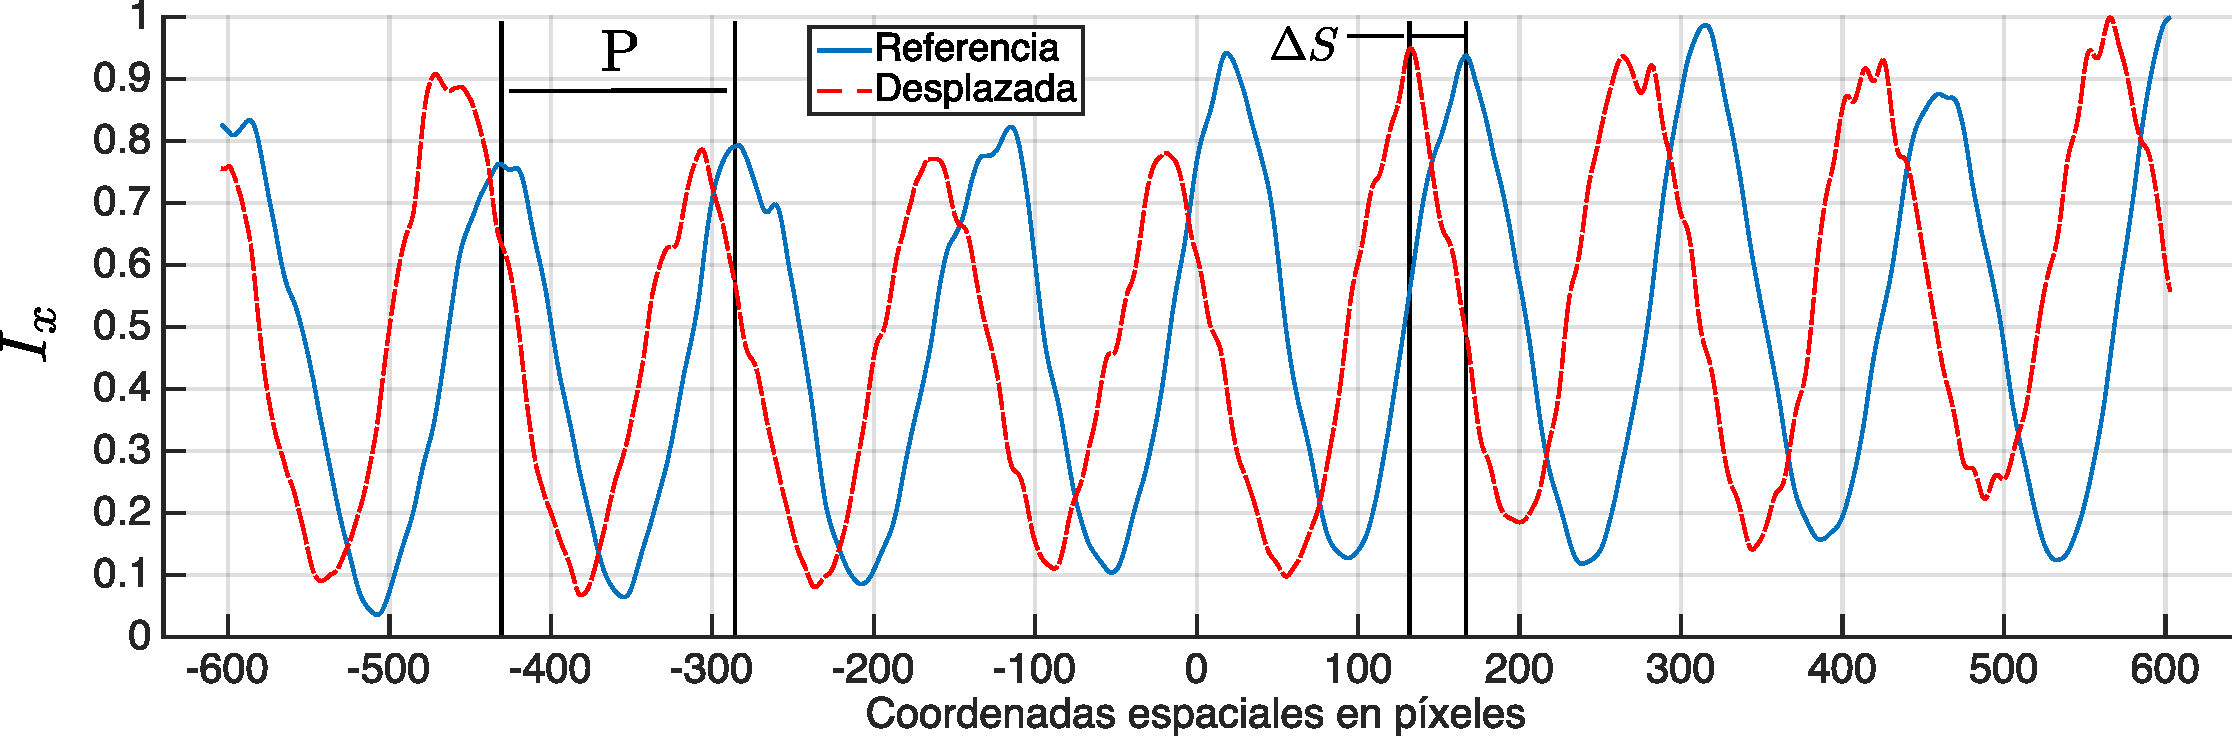
\includegraphics[scale=0.4]{fringes_plot_edited.pdf}
\caption[Patrones de interferencia 1D de interferogramas con y sin
desfase]{Patrones de interferencia 1D suavizados de los interferogramas con y sin
  desfase de la Fig. \ref{fig:split}. La imagen original tiene 1208
  píxeles y se tomó la mitad como cero.}
\label{fig:fringes_plot}
\end{figure}
La diferencia de fase $\Delta\phi$ puede ser extraída de los
interferogramas midiendo el periodo (P) y la distancia entre crestas ($\Delta S$) de la imagen de
referencia y la imagen desplazada haciendo el siguiente cálculo \citepChGen{Ma2010},
$$\Delta\phi = 2\pi \Delta S/P.$$
%De los datos en esta representación, se puede extraer la diferencia de
%fase $\Delta \phi$ a partir del periodo ($P$) sabiendo que $$\Delta
Extraer la fase de esta forma resulta bastante directo e intuitivo,
pero se aprovecha muy poca información de la señal y se pierde
precisión en comparación con otras alternativas. Además, este método resulta dificil de
programar en forma de un algorítmo. 

Otra forma de extraer la fase consiste en aplicar una \textbf{Transformada de
Fourier} (FT) a las señales e identificar los picos correspondientes a
la función seno o coseno asociada al patron de interferencia. La fase
de cada interferograma es la fase o ángulo del número complejo 
correspondiente al mayor pico de la FT una vez se ha filtrado el delta
de Dirac central correspondiente a la FT de la intensidad de fondo.  
Los picos se pueden identificar calculando el valor absoluto de la FT de
la señal y buscando el elemento más grande. La representación gráfica
de la FT se ilustra en la Fig. \ref{fig:fringes_f} con respecto a las
coordenadas de frecuencia espacial, y se observa claramente que se ha
filtrado el pico central y que la información de la FT se encuentra
alrededor de los picos en las frecuencias  8 y -8. Nosotros adaptamos
una implementación en Matlab de este método que fue inicialmente
propuesta para esta aplicación por el profesor Alberto Lencina del Centro de
Investigaciones Ópticas de Argentina. En la figura \ref{fig:fourier_script}, se muestra un
pequeño script que ilustra cómo se haría el cálculo de la fase del
interferograma de referencia.     
\begin{figure}[H]
\centering
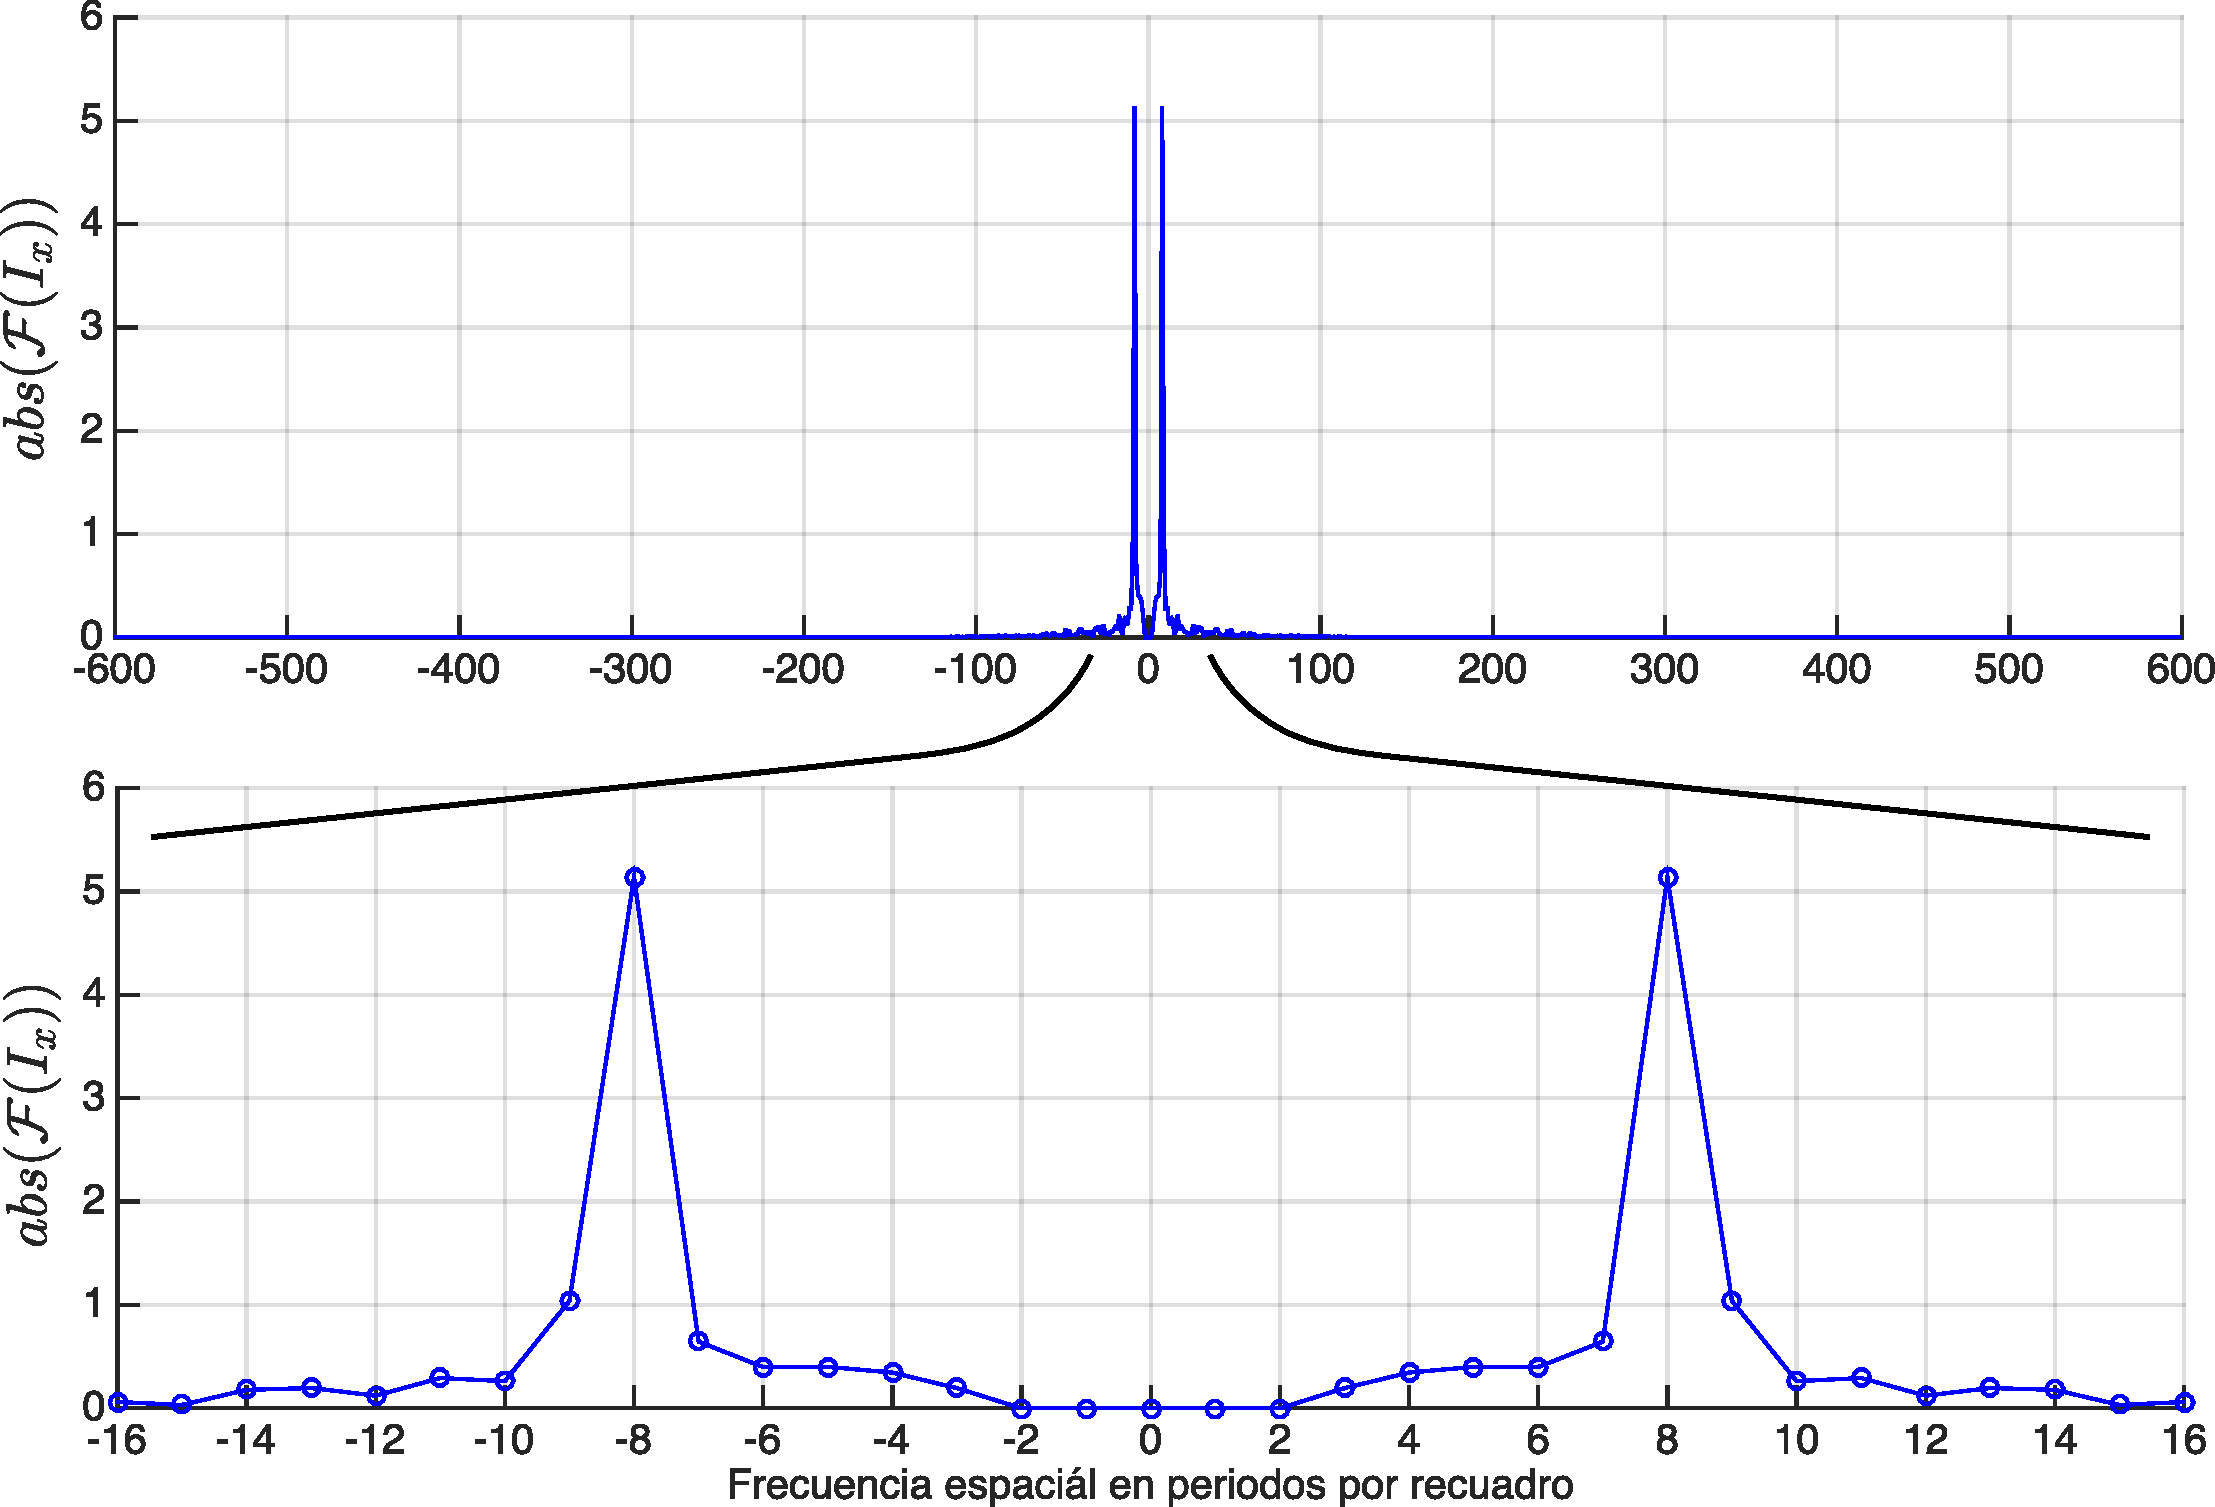
\includegraphics[scale=0.4]{fringes_f_both.pdf}
\caption[Transformada de Fourier de un patrón de
interferencia]{Transformada de Fourier del patrón de interferencia de referencia de la Fig. \ref{fig:fringes_plot}. Como es de
  esperarse para señales sinusoidales hay dos picos simétricos ambos
  lados de la coordenada frecuencial 0. Estos picos señalan correctamente que hay 8
  periodos en el interferograma.}
\label{fig:fringes_f}
\end{figure}
 \begin{figure}[H]
\begin{lstlisting}[style=Matlab]
%  Reference image
imaref=mean(imaref,1);
%  FT scaled 
TFimaref=ifftshift(fft(fftshift(imaref)));
fac=sqrt(1/(size(TFimaref,2)*size(TFimaref,1)));
TFimaref=TFimaref.*fac;
% Filtering of backround peak
radio_mask=2;
TFimaref(:,floor(size(TFimaref,2)/2)+1-radio_mask:floor(size(TFimaref,2)/2)+1+radio_mask)=0;
% Position of max value
[~, IX] = sort(abs(TFimaref),'descend');
% Phase
fase_ref =atan2(imag(TFimaref(1,IX(1))),real(TFimaref(1,IX(1))));
\end{lstlisting}
 \caption{Script para el cálculo de la fase de un interferograma usando
 FT.}
 \label{fig:fourier_script}
 \end{figure}
Si se realiza este proceso para cada una de las dos imágenes se pueden restar las
fases de ambos interferogramas y obtener la diferencia de fase
introducida por un nivel de gris particular. A diferencia del
mencionado anteriormente, este proceso es más preciso y mucho más fácil de implementar en fórma de
un algorítmo que calcule la modulación para cada nivel de gris. 
%\pagebreak
%\subsubsection{Resultados de la medida de modulación de fase}
\subsection{Resultados de la medida de modulación de fase}

Implementando el método de transformadas de Fourier como uno de los
pasos en la caracterización automatizada del SLM, se obtuvieron curvas de modulación
de fase para 60 de los 100 estados mencionados en la sección
\ref{sec:exp_validation}, correspondientes a las polarizaciones de
entrada lineales y circulares.  Las 60 curvas se han puesto al alcance del
lector en el siguiente vínculo web en forma de un notebook de IPython:
\href{http://goo.gl/RtRCX0}{\textbf{http://goo.gl/RtRCX0}}.  

Con estos datos, y con las curvas de modulación de amplitud pudimos
seleccionar una combinaciones de PSD y PSG que tiene condiciones
suficientes para usar el SLM dentro del rango de operación
deseado. Observamos que tal y como se ha reportado en la literatura,
estos moduladores acoplan la modulación de fase con la modulación de
amplitud, y que al menos con nuestro SLM no es posible encontrar
estados en los cuales el SLM sea transparente al variar niveles de gris y al mismo
tiempo permita modulaciones de fase de rango superior a $1.3\pi$.  
Encontramos que el estado 6 (Fig. \ref{fig:amp_and_phase_I6}) produce
modulaciones de fase con rango de modulación muy alto, de casi $1.9\pi$
radianes, y que, sin embargo, está acoplado a una modulación de
intensidad de muy mala calidad en la cual la transmitancia máxima es de
un $60\%$ y se reduce hasta un $10\%$. 
\begin{figure}[H]
\centering
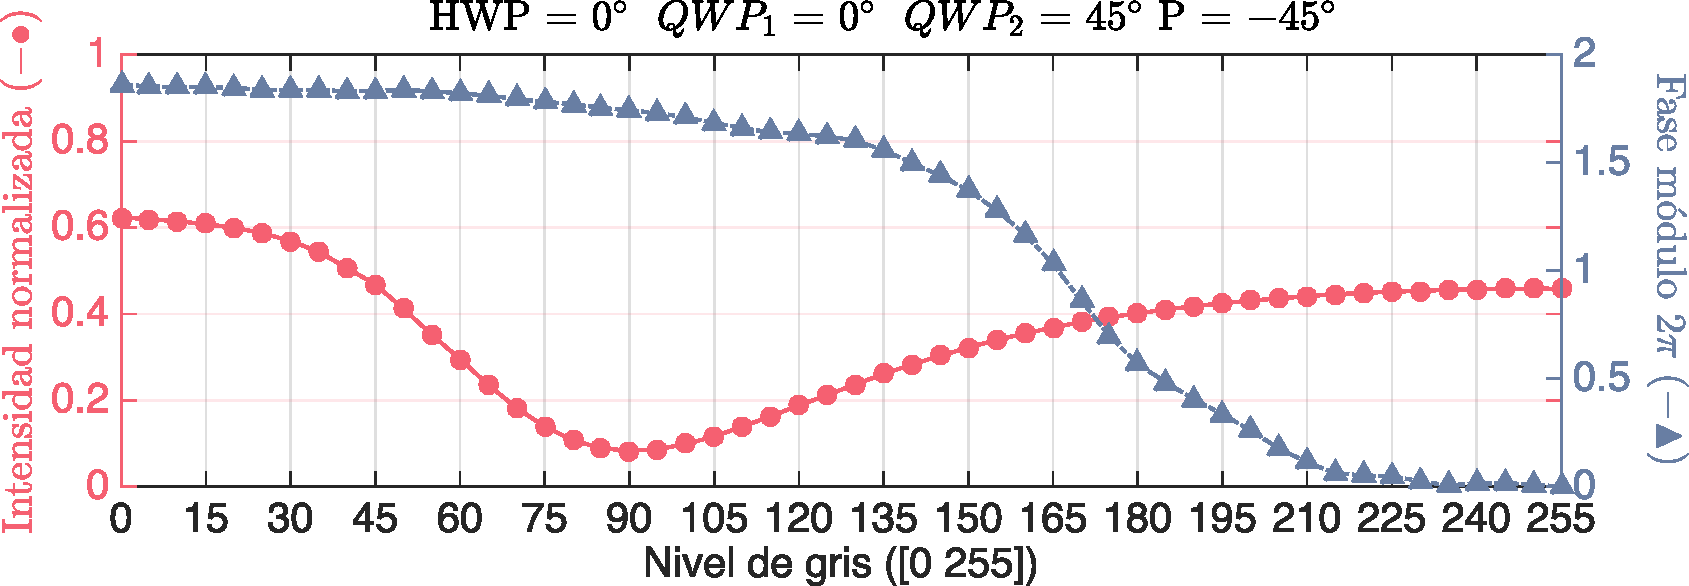
\includegraphics[scale=0.52]{amp_and_phase_I6.pdf}
\caption[Modulación de amplitud y fase del estado con máximo rango de
fase]{Posición de elementos ópticos y curvas de modulación de amplitud
  y fase del BraKet 6 que es el estado con máximo rango de modulación
  fase encontrado.} 
\label{fig:amp_and_phase_I6}
\end{figure}
%Insertar figura con comparación de modulación de amplitud y fase.
Asimismo encontramos varios BraKets en los cuales hay transmitancia
máxima con modulación de amplitud mínima, pero sufren de una muy mala
modulación de fase. Ejemplo de ellos es el BraKet 43
(Fig.~\ref{fig:amp_and_phase_I43}), que tiene alta 
transmitancia, alrededor de $10\%$ de modulación de amplitud y una
 modulación de fase casi nula. Es decir que este SLM es básicamente
 transparente ante la generación y detección estados circulares.
\begin{figure}[H]
\centering
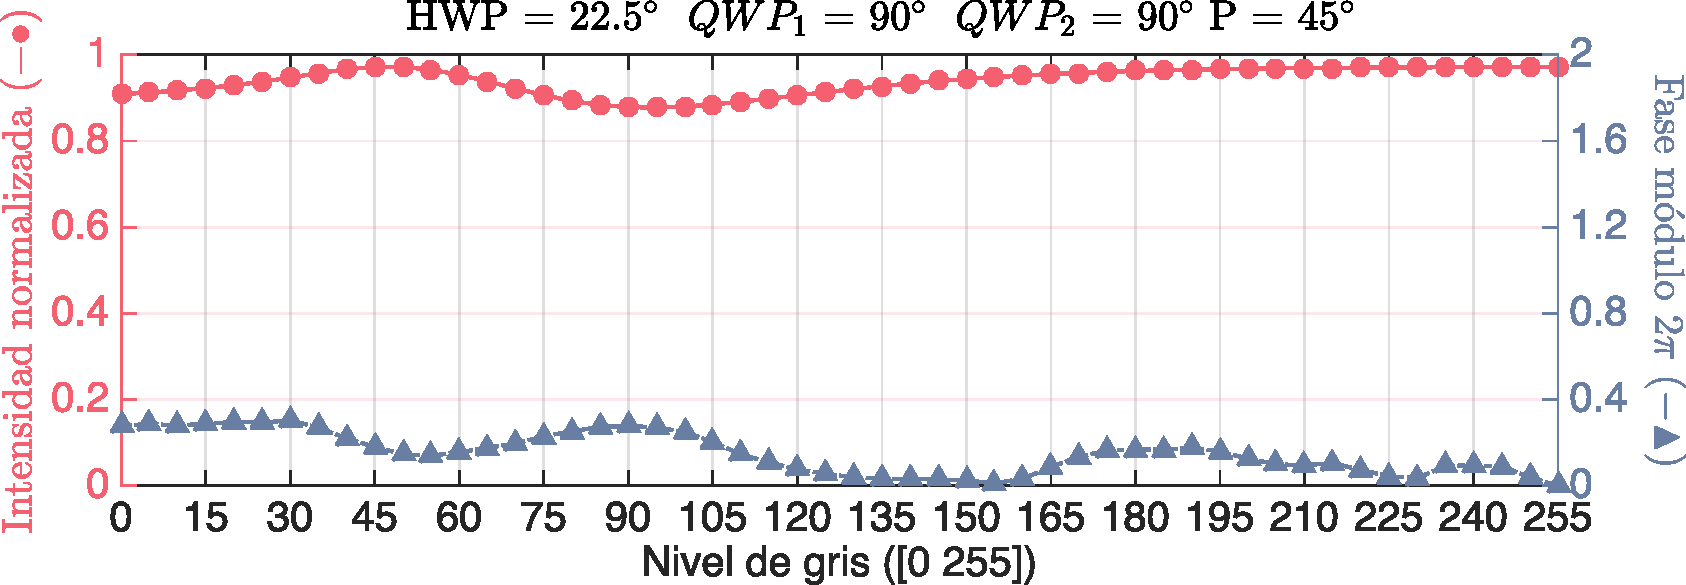
\includegraphics[scale=0.52]{amp_and_phase_I43.pdf}
\caption[Modulación de amplitud y fase del estado con mínima
modulación de amplitud]{Posición de elementos ópticos y curvas de modulación de amplitud
  y fase del BraKet 43 que es uno de los estados con mínimo rango de modulación
  amplitud.} 
\label{fig:amp_and_phase_I43}
\end{figure}

A diferencia de estos puntos extremos, en la configuración que
seleccionamos para la generación de OVs hay un compromiso de uno de
los dos fenómenos. El BraKet seleccionado es el número 10 de la
Fig. \ref{fig:braket_100_notation} que corresponde a un estado
horizontal $\mathbf{H}$ a la entrada y elíptico a $\mathbf{-45^{\circ}}$ a la
salida, las posiciones de los elementos ópticos que lo generan y las
curvas de modulación se presentan en la
Fig. \ref{fig:amp_and_phase_I100}. 
En este estado la transmitancia es baja
($~45\%$) y la modulación de amplitud es relativamente baja ($<20\%$),
pero el rango de modulación de fase es de casi $1.6\pi$ radianes, cosa que como
veremos adelante, resulta suficientemente alta para la generación de
OVs. 
\begin{figure}[H]
\centering
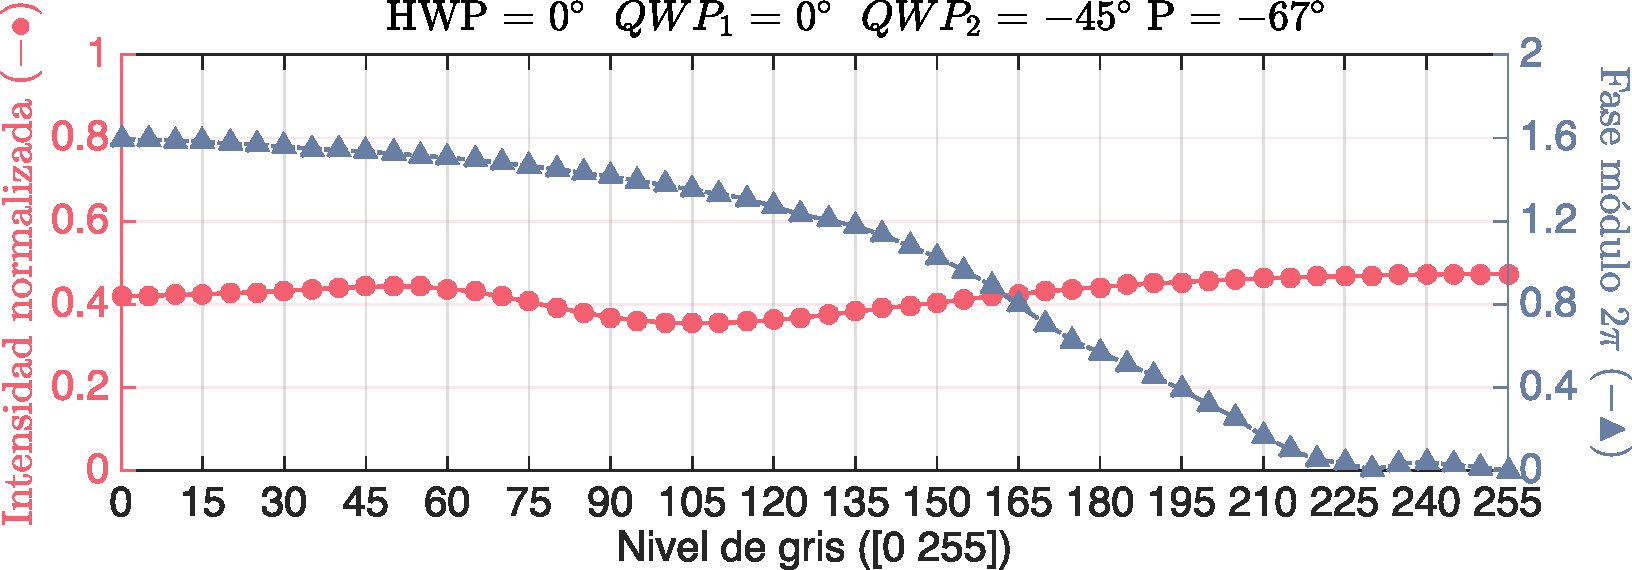
\includegraphics[scale=0.52]{amp_and_phase_I10.pdf}
\caption[Modulación de amplitud y fase óptima]{Posición de elementos
  ópticos y curvas de modulación de amplitud y fase del BraKet 10 que
  se identificó como la configuración óptima para la generación de OVs.} 
\label{fig:amp_and_phase_I100}
\end{figure}

En un principio se pensó que una forma efectiva de encontrar un estado
óptimo podía ser usando un método de minimización similar al que se
usó para encontrar los parámetros de la matriz de Jones. Tál método se
implementó con una función de minimización inspirada en la propuesta
por \citetChGen{Moreno2003} que buscaba simultaneamente
una alta tramitancia, baja modulación de amplitud y alto rango de
modulación de fase. Este planteamiento tiene varios problemas, uno de
ellos es que el espacio de valores de la función para cada
combinación de posibles estados PSG y PSD no es convexo. Es decir que
dependiendo de la semilla usada uno puede obtener un BraKet que
minimice la función de forma local, y que aún así tenga desempeño
regular. Esto se vio en diferentes ocaciones cuando medimos
experimentalmente los BraKets propuestos por las simulaciones. 
Otro problema, es que el tiempo invertido tratando de proponer
manualmente valores de peso que den mayor o menor importancia a la
sensibilidad de los parámetros con respecto a su efecto sobre la
modulación de fase o la de amplitud es excesivo. Generalmente ocurre
que la minimización 
converge a estados circulares que tienen muy buena transmitancia y
baja modulación de amplitud pero mínima modulación de fase. Y si se
modifican ligeramente los factores de peso, la minimización retorna
modulaciones de fase de menos de $1.3\pi$ con modulaciones de amplitud
de entre $15$ y $40\%$. Esto no es mejor al resultado de la
Fig. \ref{fig:amp_and_phase_I100}. Por último, encontramos que las
modulaciones de fase predichas por medio de simulaciones con las
matrices encontradas no predicen con suficiente exactitud muchas de las
modulaciones de fase registradas en el laboratorio. Esto sucede porque los
cambios de estado de polarización introducidos por el SLM afectan el
contraste de las franjas debido a la interferencia destructiva que
sucede con el haz de referencia del interferómetro
Mach-Zehnder. Ante interferogramas como el de la
Fig.~\ref{fig:fringes}(b) el algoritmo de reconstrucción de fase no
tiene como detectar la diferencia de fase entre medidas porque se
pierden las franjas.

Al final, dado que el interés fundamental de este proyecto radicaba en generar
OVs, y no en desarrollar metodos de caracterización, nos resultó mejor
seleccionar el mejor de los 100 estados disponibles (encontrados sin
dificultad por el instrumento de automatización), 
que manipular funciones de peso hasta encontrar un estado simulado con
las condiciones deseadas.

En adelante se mostrará la aplicación que desarrollamos para proyectar
máscaras de fase arbitrarias al SLM, y se mostrarán los OVs que se
pueden generar con un SLM calibrado para la modulación de fase. 

\chapter{Generación de Vórtices Ópticos}
\label{sec:OV_gen}

Como se mencionó en la sección \ref{sec:ChGen_marco_teorico}, para generar un haz
Laguerre-Gauss sólo basta propagar un haz gausiano por una máscara de
fase espiral como la de la Fig.~\ref{fig:oam_intro}b). Si se usa este 
tipo de máscaras y se añade una lente al brazo objeto del montaje de
la Fig.~\ref{fig:oam_intro} la intensidad del haz \acrshort{LG} en un
plano imagen se puede observar 
como una \textbf{función de dispersión de punto} (\acrshort{PSF}) en forma
de anillo.  

Los VOs son haces de luz que portan OAM definido a lo largo del eje.

Este tipo de OVs puede ser descrito en forma matemática como, 

El término $\exp{(il\phi)}$ introducido por las m'ascaras de fase, está asociado al valor del
\acrshort{OAM} que porta el haz, y es el responsable tanto de la
estructura helicoidal de la fase como de la singularidad 'optica a lo
largo del eje de propagaci'on \citepChGen{Padgett1999}.   


Dónde $l$ esta asociado al número cuántico del momento angular portado
por el haz, y esta relacionado con...


El momento angular orbital \acrshort{OAM} que porta un haz con
vorticidad óptica está cuantizado por el número entero $l$.  
 
La carga topologica $l$ del VO, es una propiedad  depende de la cantidad de veces que la fase
de la máscara varíe entre $0$ y $2\pi$. 
\pagebreak
\begin{figure}[H]
\centering
\includegraphics[scale=0.4]{mask_app.png}
\caption[Plataforma para la generación de máscaras de fase]{Plataforma
  para la generación de máscaras de fase a ser proyectadas en un SLM, desarrollada y registrada por el
  grupo de Óptica Aplicada de la Universidad EAFIT.} 
\label{fig:mask_app}
\end{figure}

\begin{figure}[H]
\centering
\includegraphics[scale=0.4]{OV_I10.pdf}
\caption[Vórtices ópticos obtenidos en la configuración en linea para
el BraKet 10]{Vórtices ópticos de carga topológica $l=1...4$ obtenidos
  en la configuración en linea usando los estados PSG y PSD del BraKet 10.} 
\label{fig:VOs_I10}
\end{figure}

\begin{figure}[H]
\centering
\includegraphics[scale=0.4]{OV_I6.pdf}
\caption[Vórtices ópticos obtenidos en la configuración en linea para
el BraKet 6]{Vórtices ópticos de carga topológica $l=1...4$ obtenidos
  en la configuración en linea usando los estados PSG y PSD del BraKet 6.} 
\label{fig:VOs_I10}
\end{figure}

\begin{figure}[H]
\centering
\includegraphics[scale=0.35]{diffracted_OV_I6_and_I10.pdf}
\caption[Vórtices ópticos difractados por una rejilla tipo
blazed.]{Comparación de Vórtices ópticos de carga topológica $l=1...4$ obtenidos en
  la configuración fuera de linea usando los estados PSG y PSD de los
  BraKets 10 y 6.} 
\label{fig:diffracted_OV_I6_and_I10}
\end{figure}
\newpage
\pagebreak[4]
\bibliographystyleChGen{ezspanish}
\bibliographyChGen{References/Ch2}

%: ----------------------- Parte II ------ ------------------------
\part{Caracterización y corrección de aberraciones de VO\label{ParteII}}
% this file is called up by thesis.tex
% content in this file will be fed into the main document

%------------------------------------------------------------------------- 

\chapter{Caracterización de aberraciones en Vórtices Ópticos}
\label{cha:Car_intro}
\graphicspath{{Figures/chPD_img/}{../Figures/chPD_img/}}
\lhead{Caracterización de aberraciones en Vórtices Ópticos:
  \textit{Introducción}} % This is for the header on each page -
                         % perhaps a shortened title
\section{Introducción}
En capítulos anteriores ha quedado claro que para producir VO es
necesario contar con un sistema óptico en el cual sea posible
manipular con precisión la fase de un frente de onda.  Asimismo, se
presentó un montaje experimental en el cual logramos generar VO a
partir del uso de dispositivos difractivos conocidos como SLMs. 
No obstante, los VO obtenidos distan de ser de suficiente calidad como
para ser usados en aplicaciones científicas o tecnológicas. 

Esta segunda parte de la tesis abarca el trabajo que se realizó para
mejorar la calidad óptica de nuestro montaje con el fin de mejorar los
VO que se obtuvieron en la parte anterior. 

\section{Estado del Arte}
\label{sec:ChPD_estado_del_arte}
\lhead{Caracterización de aberraciones en Vórtices Ópticos: \textit{Estado
    del Arte}}

Los sistemas ópticos formadores de imagen que se encuentran en
aplicaciones de la vida real están sujetos a aberraciones de fase que
limitan su resolución. Es por ello que en la industria y en laboratorios se hace un gran esfuerzo para
detectar aberraciones y corregirlas vía Óptica Adaptativa (AO) \citepChPD{Kubby2013} o por
medio de técnicas digitales posteriores a la adquisición
\citepChPD{Korkiakoski2012}. 

Las aberraciones ópticas en un sistema formador de imagen pueden
proceder de fuentes intrínsecas tales como imperfecciones en el
diseño, los materiales, la manufactura o la alineación de los
elementos que los componen. O de fuentes extrínsecas como variaciones
en el índice de refracción de muestras microscópicas y turbulencia atmosférica en
imágenes capturadas usando telescopios. La presencia de aberraciones
del último tipo en imágenes procedentes de telescopios terrestres, y
la dificultad de modificar los sistemas para incluir brazos de referencia han sido la motivación para
el desarrollo de varias técnicas de Sensado de Fase no
Interferométricas (NI-WFS). La técnica de Diversidad de Fases o Phase
Diversity (PD) pertenece a una familia de NI-WFS conocida como de
Reconstrucción de Fase o Phase Retrieval. A diferencia de técnicas
directas que requieren de óptica y sensores adicionales como los
sistemas que usan sensores Shack-Hartman, las técnicas de Phase
Retrieval consisten en la determinación de la fase de una función
compleja a partir de medidas de su magnitud usando 
información a priori de la función o de su transformada \citepChPD{Fienup1993}. 
Específicamente, la técnica de reconstrucción  PD ha sido usada
exitosamente en el contexto de sistemas de AO para incrementar la resolución de sistemas ópticos
tales como el Telescopio Espacial Hubble \citepChPD{Fienup1993}, y en
post procesamiento de imágenes de astronomía en las cuales la
resolución es crítica. Dos casos muy relevantes son el estudio de
manchas solares y la detección de planetas extrasolares \citepChPD{Lofdahl1994,Bonet2005,Korkiakoski2012,Sauvage2007,Sauvage2012}. 
Así como con otras técnicas desarrolladas para aplicaciones en
astronomía, los métodos de reconstrucción de fase como el
Gerchberg-Sachston (GS) y PD han migrado a aplicaciones en el
laboratorio, y más específicamente a aplicaciones en microscopía de
fase \citepChPD{Jesacher2007,Camacho2010,Kner2013a}. Tal es el caso
del trabajo de \citetChPD{Jesacher2007} que implementó una versión del
método GS para la optimización de pinzas ópticas utilizadas como
iluminación en sistemas de microscopía de contraste de fase espiral. \\
En este capítulo se presenta un método novedoso de reconstrucción de
fase del tipo PD inspirado en la aplicación antes mencionada, y por
medio del cual fue posible detectar y corregir las aberraciones ópticas
del sistema generador de VO presentado en el capítulo
\ref{cha:Gen_intro}.  A continuación, se presenta el marco teórico que
soporta la implementación del método. En la sección
\ref{sec:ChPD_materiales_y_metodos} se presenta el montaje óptico y se
describe el algoritmo general para la reconstrucción de fase. Lugo, en
la sección \ref{sec:ChPD_resultados} se presentan los resultados de
simulaciones y experimentos que permiten corroborar la efectividad del
método para la corrección de aberraciones. 

\section{Marco Teórico}
\label{sec:ChPD_marco_teorico}
Los métodos de reconstrucción de fase no interferométricos dependen de
la medida de la intensidad de la intensidad del campo óptico que se
propaga a traves de un sistema formador de imagen. Si el sistema
formador de imagen se
caracteriza por su Función de Dispersión de Punto (PSF), la intensidad
a la salida puede ser descrita como una convolución entre la imagen a
la entrada y la PSF tal y como se ilustra en la ecuación
(\ref{eq:Output_Image}).
\begin{equation}\label{eq:Output_Image}
d(\vec{x}) = d_{obj}(\vec{x}) \otimes s(\vec{x}).
\end{equation}
En este caso hemos usado la notación de \citetChPD{Paxman1992} dónde
la PSF se representa como $s$, $d_{obj}$ es la intensidad del objeto a
la entrada y $d$ es la intensidad de la imagen a la salida, todas
ellas evaluadas en el espacio de coordenadas naturales ($\vec{x}$). El
 \href{http://es.wikipedia.org/wiki/Teorema_de_convolución}{Teorema de
   Convolución} permite representar la operación de la expresión
 (\ref{eq:Output_Image}) como un simple producto punto entre las
 Transformadas de Fourier (FT) de la intensidad a la entrada y la
 PSF como se muestra a continuación. 
\begin{equation}\label{eq:Output_Image_fourier}
D(\vec{u}) = D_{obj}(\vec{u})S(\vec{u}).
\end{equation}
En \ref{eq:Output_Image_fourier} el término $S$ denota la Función de
Transferencia Óptica (OTF) del sistema formador de imagen, y así como
con los otros términos, letras mayúscula denotan una transformada de
Fourier sobre la función con notación minúscula.
\begin{align*} 
S(\vec{u})&= \mathcal{F}\{ s(\vec{x}) \},&D(\vec{u})&= \mathcal{F}\{ d(\vec{x}) \}, &D_{obj}(\vec{u})&= \mathcal{F}\{ d_{obj}(\vec{x}) \}. 
\end{align*}
Hasta el momento hemos trabajado únicamente con funciones reales que
representan la intensidad del campo punto a punto en los planos objeto
e imagen de un sistema óptico. Este tipo de notación es de gran utilidad para las
aplicaciones clásicas del método PD que hacen imagen de objetos
lejanos, y con fuentes de iluminación no coherentes. Sin embargo, en
sistemas ópticos con fuentes de iluminación coherentes, como el que se presentó en la primera parte de este documento
para la generación de VO, tenemos la ventaja de trabajar con
campos complejos que proporcionan información de amplitud y fase. Para
adaptar el método clásico de PD a una versión de iluminación coherente
es necesario trabajar con campos complejos. Es bien sabido que la OTF
y la PSF forman un par de Fourier en el dominio no coherente, y cada
una de ellas tiene un equivalente en el dominio de la luz
coherente. Por una parte, la contraparte coherente de la PSF es la
Función de Respuesta al Impulso en amplitud o PSF de amplitud y de
aquí en adelante se denotará como $h(\vec{x})$. La PSF es el módulo
cuadrado de la PSF de amplitud (APSF), 
\begin{equation}\label{eq:PSF}
s(\vec{x}) = |h(\vec{x})|^2.
\end{equation}
Y así
como la PSF relaciona intensidades de campo a la entrada y salida de
un sistema por medio de una convolución, la PSF de amplitud relaciona
los campos ópticos complejos.
 \begin{equation}\label{eq:Output_Image_complex}
u(\vec{x}) = u_{obj}(\vec{x}) \otimes h(\vec{x}).
\end{equation}
Del otro lado, el equivalente coherente de la OTF es la Función de
Transferencia Óptica de amplitud, o Pupila Generalizada del sistema
(GP) y por ser el par de Fourier de la APSF se cumple la relación (\ref{eq:GP}). 
\begin{equation}\label{eq:GP}
 H(\vec{u}) = \mathcal{F} \{h(\vec{x})\} =  A(\vec{u}) e^{i\phi(\vec{u})}
\end{equation}
En (\ref{eq:GP}) se observa que fuera de ser la FT de la APSF, la GP es
una función compleja que describe tanto la forma y
tramitancia de la apertura $A(\vec{u})$ como la fase introducida por sistema
óptico $\phi(\vec{u})$. Esta fase generalmente es sinónimo de las
aberraciones del sistema y se describe matemáticamente de forma
parametrizada como una combinación de polinomios de polinomios de Zernike.\\
La OTF de un sistema formador de imagen con iluminación coherente se
puede obtener mediante la autocorrelación normalizada de la GP como se
muestra a continuación.
\begin{equation}\label{eq:OTF}
S(\vec{u}) = \frac{H(\vec{u}) \star H(\vec{u})}{|H(\vec{u})|^2}
\end{equation}
Todo lo mencionado anteriormente ha sido ingeniosamente condensado por
\citetChPD{UribePatarroyo2011} en una versión de la figura
\ref{fig:ChPD_kernels_sistemas_formadores_de_imagen}. 
\begin{figure}[h!]
\centering
\includegraphics[scale=.8]{kernels_sistemas_formadores_de_imagen.pdf}
\caption[Relaciones entre funciones de transferencia ópticas y sus FT.]{Relaciones entre funciones de transferencia ópticas y sus
  transformadas de Fourier en los dominios coherente y no
  coherente. Inspirado en una versión similar de \citetChPD{UribePatarroyo2011}.}
\label{fig:ChPD_kernels_sistemas_formadores_de_imagen}
\end{figure} 
Ahora bien, las expresiones (\ref{eq:PSF}) y (\ref{eq:OTF}) nos
permiten llevar sistemas ópticos descritos por campos complejos a la
notación tradicional del PD. A continuación se describen los aspectos
 generales de la reconstrucción de fase con PD, en la sección
 \ref{sec:ChPD_PD_il_coherente} se describirán las modificaciones que
 hacemos al PD tradicional para aprovechar el tipo de iluminación no
 coherente, y en la sección \ref{sec:ChPD_PD_Spiral_Diversity} se
 explica el efecto de introducir máscaras espiral como diversidades de
 fase. 

\subsection{PD tradicional}
\label{sec:ChPD_PD_tradicional}
Si la GP del sistema es modificada por un cambio conocido en la fase o
diversidad de fase de la forma:
$$H_{\Delta}=e^{\phi_1(\vec{u})}.$$ 
Obtenemos una nueva GP que se puede describir como el producto entre
la GP original ($H_{0}$) y la GP con el cambio o diversidad de fase
($H_{\Delta}$). Estas diversidades son generalmente desenfoques
introducidos al cambiar el camino óptico de haces esféricos, o pueden
ser otro tipo de distribuciones de fase fácilmente parametrizables en
polinomios de Zernike como el astigmatismo. Tomando la autocorrelación normalizada de la GP con
diversidad como se muestra en la expresión (\ref{eq:first_diversity_OTF})
\begin{equation}\label{eq:first_diversity_OTF}
S_1 = \frac{H_1\star H_1}{|H_1|^2} = \frac{H_0H_{\Delta} \star H_0H_{\Delta}}{|H_0H_{\Delta}|^2}
\end{equation}
obtenemos una OTF con diversidad $\phi_1$ que nos permitirá predecir cómo son
las imagenes registradas a la salida del sistema cuando se introduce
un cambio de fase: $$D_1 = D_{obj} S_1.$$ 
La tarea de encontrar las aberraciones del sistema óptico en el PD
tradicional consiste entonces en encontrar una distribución de fase
inicial $\phi(\vec{u})$ que en combinación con la función pupila
$A(\vec{u})$ componga una OTF capaz de modelar el
sistema. Esta OTF debe predecir, a partir de una entrada dada 
($D_{obj}$)  no solo la imagen nominal ($D_0$), sino tambien
las imágenes distorsionadas $D_{1...k}$ que resultan de la adición de
$k$ diversidades de fase distintas. Y la adición de más de una
diversidad de fase es la que diferencia al método PD de métodos
similares, en particular, la inclusión de diversidades implica que la
fase del frente de onda recuperado debe ser una solución para un
conjunto de sistemas y no sólo para uno, esto le otorga al método una
mayor precisión.  La fase del frente de onda a recuperar puede ser
encontrada utilizando Algoritmos de Propagación Iterativos como el GS o por
métodos de búsqueda basados en el Gradiente \citepChPD{Fienup1993}.
Las implementaciones de PD basadas en algoritmos de búsqueda del
gradiente usan métodos de búsqueda de la mayor pendiente para
minimizar funcionales de la forma:
\begin{equation}\label{eq:metric}
L(\bar{D}_{obj}, \phi)= \sum_{j=0}^{K} \sum_{u,v}^{M,N}  \left |D_{j} - \bar{D}_{obj} S_{j} \right | ^2.
\end{equation}

Dónde $\bar{D}_{obj}$ es la FT del objeto a la entrada limitada por las frecuencia
de corte establecidas en la apertura, y $D_{j}$ es la FT de la intensidad
medida experimentalmente por una cámara en el pixel con coordenadas $(u,v)$ luego de
introducir una diversidad de fase conocida con índice $j$.      
Este funcional actua como una medida de la similitud entre la
intensidad de un objeto que se propaga por un sistema modelado por
$S_{j}$ y la medida real de su imagen. Obtener un valor mínimo al
evaluar el funcional para todas las diversidades $j$ implica que el objeto a la entrada y la OTF del
sistema se conocen de forma suficientemente precisa como para emular
el sistema real.   

Es importante fijarse en que el funcional clásico de PD
(\ref{eq:metric}) debe solucionarse simultaneamente con respecto a dos
variables. Esto se debe a que en aplicaciones de PD para sensado
remoto se desconoce tanto la fase introducida por el sistema, como las
propiedades del objeto a la entrada. Puesto que solucionar un funcional
simultaneamente para dos funciones resulta complejo y muy costoso
computacionalmente, desde los inicios de la técnica autores como \citetChPD{Gonsalves1982} han propuesto
una transformación de (\ref{eq:metric}) que permite describir el funcional sólo en términos
de la fase del frente de onda. Esta transformación está descrita
de forma muy completa y generalizada en el trabajo de \citetChPD{Paxman1992}, y ha
sido implementada exitosamente por \citetChPD{Katkovnik2012}. No
obstante, ha sido demostrado que la forma reducida del funcional es
mucho más susceptible a devolver mínimos locales en la presencia de
ruido Gaussiano, y por tanto se ha propuesto el uso de métodos de
regularización y metaheurísticos para incrementar la convergencia.  

En la siguiente sección se propone una modificación al PD clásico que
soluciona estos problemas con la condición de limitar el método a
rangos de aplicación en los cuales es posible conocer el frente de
onda a la entrada del sistema óptico. 

\subsection{PD con iluminación coherente}
\label{sec:ChPD_PD_il_coherente}

La variación de PD que nosotros proponemos puede llamarse PD con
iluminación coherente, y requiere de 
conocer el frente de onda a la entrada del sistema. En nuestro caso,
como los VO van a ser generados para aplicaciones en microscopia,
el sistema óptico es un microscopio 4F compuesto por dos lentes. 
 Dado que en el montaje que usamos para generar VO usamos una fuente laser, podemos asumir que el campo óptico a la entrada ($u_{obj}$) se puede representar
como un haz de luz coherente con perfil Gaussiano y frente de onda
plano. 
$$u_{obj} = e^{\frac{-(x^2+y^2)}{\sigma}}.$$
 Ese sería el campo óptico a la entrada del 4F, es decir, a una distancia focal de la primera lente. La FT del
 objeto ($U_{obj}$) con coordenadas de frecuencia espacial puede ser
 observada en el plano focal de la
 primera lente (2F), y el campo a la salida del sistema está de nuevo
 en coordenadas naturales y se puede observar a 4 distancias
 focales. Si se define la GP en términos de la apertura en el dominio de Fourier, y
 la fase de la GP se asocia a la fase introducida
 tanto por aberraciones del sistema como por las diversidades, el
 campo a la salida se puede expresar en términos del campo a la
 entrada como se muestra en la ecuación \ref{eq:field}.
\begin{equation}\label{eq:field}
u_{j}(\vec{x}) = \mathcal{F}^{- 1}\{ U_{obj} H_0(\vec{u}) H_j(\vec{u}) \}.
\end{equation} 
Con la expresión (\ref{eq:field}) se puede plantear un equivalente coherente del
funcional (\ref{eq:metric}) en el cual la única incógnita son las
aberraciones introducidas por el sistema óptico.
\begin{equation}
L_j(\phi)= \sum_{j=0}^{K} \sum_{u,v}^{M,N}  \left |d_{j} - |u_j|^2
\right | ^2.
\label{eq:metric_coherent}
\end{equation}
Si la apertura es circular y el objeto es un haz Gaussiano con frente
de onda plano, las distribuciones de intensidad a la salida para cada diversidad ($d_{j}$)
son patrones de Airy distorsionados 
localizados en el centro de la imagen.  
Es importante notar que a diferencia del PD tradicional, nosotros
comparamos las imágenes en coordenadas naturales en vez del dominio de
frecuencia espacial. Esto se debe a que el sistema formador de
imágenes es un 4F. Otra diferencia muy importante es que podemos saber
cómo será la fase a la salida, cosa que no se podría hacer con
iluminación no coherente. Esto es esencial si queremos garantizar un
perfil de fase específico como por ejemplo una vorticidad particular. 

\subsection{Máscaras espirales como diversidades de fase}
\label{sec:ChPD_PD_Spiral_Diversity}
Como se mencionó en la introducción, \citetChPD{ Jesacher2007}
propusieron el uso de máscaras espirales para mejorar el desempeño en
la reconstrucción de aberraciones por medio del método GS en un
sistema formador de imagen. El GS es un método iterativo de
reconstrucción de fase que funciona con sólo una imagen como
entrada. En ese trabajo mostraron que si el sistema
óptico se ilumina con haces portadores de OAM 1, la imagen a la salida
(que tiene forma de dona) responde con mucha mayor sensibilidad a aberraciones que las
imagenes observadas cuando la iluminación es de fase plana (OAM 0). Ese
incremento en la sensibilidad se ve traducido en una mayor
precisión, y en un aumento en la convergencia que hacen del método una alternativa
atractiva para la optimización de sistemas ópticos en los cuales se
necesita contról preciso de la fase. 

Los resultados de \citetChPD{ Jesacher2007} pueden ser extendidos al
método de PD con iluminación coherente si se modifica el funcional (\ref{eq:metric_coherent}) de la
sección \ref{sec:ChPD_PD_il_coherente} para recibir una nueva familia de
diversidades de fase que introduzcan OAM al haz de entrada. \\
Estas diversidades son máscaras espiral de fase parametrizadas por el
valor de su carga topológica $l$ y definidas como:

$$\psi_l = arg(\exp{(il \theta)})$$

tal y como se mostró en la sección (referenciar la sección en la que
se habla del programa para generación de máscaras). 

Al incluir las máscaras espiral en un plano de Fourier del sistema, la fase del frente de
onda se puede representar aproximadamente suma de:
\begin{itemize}
\item Las aberraciones inherentes al sistema ($\phi$) representadas como una
  combinación ponderada de polinomios de Zernike. En nuestro caso la
  combinación se hace con los primeros 15 coeficientes siguiendo la
  convención de numeración de \citetChPD{Noll1976}. 
\item La diversidad de fase espiral ($\psi_l$).
\item La diversidad de fase de aberración ($\psi_l$) que consiste en
  un solo elemento de la base de Zernike, como desenfoque o
  astigmatismo. 
\end{itemize}
El campo complejo a la salida del sistema cuando se introduce una diversidad de
aberración $j$ y una diversidad de espiral de fase $l$ en un plano de
Fourier es entonces:
\begin{equation}\label{eq:newGP}
 u_j^l =  \mathcal{F}^{- 1}\{U_{obj} A e^{i\left(
     \phi+ \psi_l + \phi_j \right)} \}.
\end{equation}

Usando la ecuación (\ref{eq:newGP}) se puede definir el funcional de
PD coherente mejorado con VO que se muestra en la ecuación
(\ref{eq:metric_coherent_OAMs}). %a continuación:
\begin{equation}\label{eq:metric_coherent_OAMs}
L(\phi)= \sum_{l=0}^L\sum_{j=0}^{K} \sum_{u,v}^{M,N}  \left |d_{j}^l - |u_j^l|^2 \right | ^2.
\end{equation}

Con ese funcional se puede plantear una metodología de solución para
el problema de reconstrucción de fase como se ilustra en el diagrama
de flujo de la figura  \ref{fig:flowchart}.

\begin{figure}[h!]
\centering
\includegraphics[scale=1.2]{PDLightFlux_simple_esp.pdf}
\caption[Diagrama de flujo del PD con iluminación coherente]{Diagrama de flujo de una implementación de PD con iluminación
  coherente mejorado con VO.}
\label{fig:flowchart}
\end{figure}

A continuación, en lo que resta de este capitulo se ahondará en el método y en los detalles del proceso
para entender qué es lo que sucede en cada una de las etapas. 

\section{Materiales y Métodos}
\label{sec:ChPD_materiales_y_metodos}

Como se mencionó en la sección \ref{sec:ChPD_PD_il_coherente}, para
poder generar imágenes simuladas $|u_j^l|^2$ nuestro método se basa en
la premisa de conocer el campo óptico a la entrada del sistema
formador de imagen. Es decir que si usamos un láser de buena calidad
para obtener las imágenes del brazo izquierdo del diagrama
\ref{fig:flowchart} podemos asumir que el campo a la entrada del
sistema simulado ($u_{obj}$)
%que produce las imágenes del brazo derecho
, tiene las características
ópticas de una fuente láser coherente, es decir: amplitud Gaussiana, perfil
de fase plano, y que además está limitado por una
apertura circular correspondiente a la geometría de las lentes (En esta parte se podría hacer referencia a
un montaje óptico descrito en el capítulo pasado. Idealmente a una fotografía).  

Como el nuestro es un sistema formador de imagen y vamos a introducir las
máscaras de diversidades en un plano de Fourier para simular la autocorrelación, se debe obtener la
transformada de Fourier del campo mencionado anteriormente y colimar
el haz para evitar que siga divergiendo. En adelante haremos
referencia a la figura \ref{fig:set-up} para ilustrar las diferentes
partes del sistema para reconstrucción de fase como si se tratara de
un sistema 4F.
Suponiendo que el frente de onda ya ha sido transformado al dominio de Fourier y que se
encuentra colimado, representamos en el extremo izquierdo de la figura
\ref{fig:set-up} la FT del campo a la entrada ($U_{obj}$) como un haz
circular que incide sobre un TN-SLM (El mismo Holoeye 2002 que se
present[o anteriormente).  Dado que el campo ha sido
colimado luego de obtener su FT, se puede asumir que todos los planos desde que
se colima el haz hasta que vuelve a pasar por una lente son
equivalentes al plano de Fourier de un sistema 4F, y eso nos brinda un
espacio adecuado para introducir el SLM como se muestra en el recuadro
azul de la figura \ref{fig:set-up}. 

Si se trabaja en aplicaciones de microscopía en las cuales los objetos
son de tamaños micrométricos, sus transformadas de Fourier son campos
ópticos más extensos y la información en coordenadas de frecuencia
espacial puede dispersarse en tamaños comparativamente más
grandes. Una ventaja significativa de modificar el PD para que las
diversidades de fase se introduzcan en un plano de Fourier es el hecho
de que se pueden aprovechar más pixeles, y por ende se aumenta la
resolución espacial de la modulación de fase. 

%El uso de SLMS y sus ventajas. 

El uso de dispositivos de modulación espacial de la fase para
aplicaciones en PD se ha extendido en la literatura
\citepChPD{Uribe-Patarroyo2010,Camacho2010,Korkiakoski2012,Katkovnik2012}
debido a la flexibilidad con la que se pueden generar máscaras de fase
arbitrarias como diversidades de fase, a diferencia de métodos
tradicionales como desenfoques que dependen de desplazamientos y alineación muy
precisos de elementos ópticos. Más aún, el uso de elementos de
la base de Zernike (diferentes al desenfoque) como diversidad de aberración tiene la ventaja de
producir distorsiones más grandes y más facilmente detectables en la
distribución de intensidad del plano imagen. Esto es particularmente
cierto cuando los las distribuciones pertenecen a objetos altamente
sensibles a aberraciones como es el caso de los OV. Polinomios de
Zernike como los dos correspondientes al astigmatismo primario han
sido usados por \citetChPD{Kner2013} como diversidad de aberración en PD para reconstrucción de
fase de objetos tridimensionales en aplicaciones de microscopía donde
el desenfoque no añade una cantidad significante de información. 
 
\begin{figure}[h!]
\centering
\includegraphics[scale=.5]{PhaseDiversitySetup_esp.pdf}
\caption[Diagrama del sistema óptico para PD con iluminación coherente.]{Un SLM es usado para introducir diversidades de fase en un
  plano de Fourier. La máscara que se asigna al CL es una combinación de:
  (a) Máscara espiral de fase con OAM 1, (b) rejilla de difracción
  tipo Blazed, y (c) +0.5 astigmatismo primario como diversidad de
  aberración. El primer orden de difracción producido por la rejilla
  es usado como portador de los haces Laguerre-Gauss con OAM1
  enfocados en el plano imagen.} 
\label{fig:set-up}
\end{figure}

Cuando $U_{obj}$ llega al SLM se encuentra con una combinación de tres
máscaras de fase que han sido asignadas a los píxeles del CL. La
primera de estas máscaras, visible en la figura \ref{fig:set-up}(a)  es una máscara de espiral de fase con carga
topologica $l$ que (como
se vio en la sección ``referenciar sección'') introduce un una
singularidad de fase de orden $l$ al campo. La segunda máscara
(\ref{fig:set-up}(b)) corresponde a una rejilla de difracción del tipo
blazed que se usa para separar la luz que ha sido difractada al primer
orden del resto. Esta rejilla mejora de forma significativa la calidad
de los vórtices ópticos porque evita efectos de interferencia causados
por partes del campo que no son correctamente difractadas por el
modulador. La poca eficiencia de difracción se debe a la no linealidad
de la modulación y al hecho de que los TN-SLM de transmisión no logran
modulaciones de $2\pi$.  Finalmente, la tercera máscara
(Fig. \ref{fig:set-up}(c)) introduce la diversidad de fase de
aberración, en este caso, y en adelante corresponde al polinomio de
Zernike de astigmatismo primario (De índice 4 en la notación de
Noll). La suma de las tres máscaras tal y como se le presenta al SLM
en el montaje experimental se muestra en la figura
\ref{{fig:mixed_mask}} superpuesta a una
apertura circular que corresponde al tamaño del haz en el SLM.   

\begin{figure}[h!]
\centering
\includegraphics[scale=.5]{mixed_mask.pdf}
\caption[Ejemplo de una máscara tenedor con astigmatismo.]{Ejemplo de una máscara tenedor que resulta de combinar una
  máscara de espiral con $l=1$, con una red de difracción y una
  máscara de diversidad de aberración con astigmatismo primario de
  $Z_4=0.5\lambda$.} 
\label{fig:mixed_mask}
\end{figure}

Luego de atravesar el SLM el haz encuentra el resto del sistema óptico
y se enfoca para formar imagen ($|u_j^l|^2$) en el plano de observación o plano
imagen. 
% En nuestro caso el resto del sistema consiste en una sola
% lente (tal y como se muestra en alguna foto) con la misma curvatura
% que la lente usada para colimar el haz hace ima. 
Como se puede ver en el extremo derecho de la figura \ref{fig:set-up},
los perfiles de intensidad que se usan como entrada para el algoritmo
de la figura \ref{fig:flowchart} corresponden sólo a una pequeña parte
de la imagen en la cual está el orden +1 de la rejilla de
difracción. Dado que los spots tienen un tamaño microscópico, para observar sólo
el orden 1 en el plano de enfoque usamos un objetivo de 
microscopio de magnificación 10x y una cámara CCD marca Imaging
Source.    

En conclusión, para realizar la reconstrucción de fase de un sistema
óptico formador de imagen usando nuestro método, se deben registrar varias de las
imágenes que éste forma cuando se le introducen cambios conocidos en
la fase. Los cambios en la fase se introducen a partir de máscaras de
fase localizadas en uno de sus planos de Fourier por medio de un
TN-SLM.  
Introducir las máscaras de fase genera distorsiones en la distribución
a la salida que además dependen de las aberraciones ópticas desconocidas del
sistema en cuestión. El hecho de generar varias combinaciones de
diversidades y registrar varias imagenes con distorsiones distintas,
lleva a limitar el espacio de soluciones posibles y acerca el método a
una solución única. Esta es la gran ventaja del PD sobre otros métodos
de reconstrucción de fase. 

Adicionalmente, el hecho de usar la familia
de diversidades de espiral, aumenta la sensibilidad del método ante
aberraciones ya que los haces portadores de OAM tienen cambios más
drásticos en sus distribuciones de intensidad cuando hay
aberraciones. Aumentar la sensibilidad tiene un efecto positivo sobre
la exactitud de la solución porque se encuentra de forma más precisa
el valor y tipo de aberraciones que producen una distribución particular. 

El conjunto de imágenes tomadas experimentalmente ($d_j^l$), y las
condiciones particulares con las cuales fueron producidas, tales como:
la forma de la apertura, el tipo de iluminación y la selección de diversidades, son el
argumento de la rutina de PD. En el interior de la rutina de PD,
simulamos el sistema óptico y producimos imágenes artificiales
($|u_j^l|^2$) que son comparadas píxel a píxel con las imágenes
experimentales. Así como las distorsiones en las imágenes
experimentales son función de las aberraciones que desconocemos, las
distorsiones de las imágenes artificiales van a ser función de una
fase conocida y parametrizada ($\phi$) que vamos a variar hasta que el funcional
\ref{eq:metric_coherent_OAMs} retorne un mínimo. 
Cuando acabe el esquema de búsqueda de un mínimo, y la fase
propuesta ($\phi$) produzca imágenes artificiales ($|u_j^l|^2$)
idénticas a las imágenes experimentales, y siempre y cuando las
condiciones de la simulación sean idénticas a las condiciones del
laboratorio, significará que hemos identificado las aberraciones del
sistema óptico correctamente.

Una vez presentado el método, procedemos a presentar los resultados
logrados. 
%introducir un TN-SLM en un plano de Fourier 

\section{Resultados}
\label{sec:ChPD_resultados}

Nuestro método fue probado extensivamente con el fin de validar
nuestras premisas y evaluar su comportamiento ante diversas entradas. 
En esta sección se describen las pruebas simuladas y experimentales
que se realizaron, y se muestran los resultados para cada una. 

\subsection{Resultados de simulaciones}
\label{sec:ChPD_resultados_simulados}
En primera medida se requería simular el método para corroborar que
funcionaba en sistemas ideales. La simulación de reconstrucción de
fases consiste en reemplazar el conjunto de imagenes de referencia $d_j^l$ por un
conjunto de imágenes artificiales que han sido afectadas por una
aberración conocida inherente al sistema
óptico simulado. La aberración conocida será nuestra fase de
referencia, es decir, la fase con la cual compararemos la exactitud de
la reconstrucción. 
Una vez comprobamos que nuestra implementación del PD reconstruía de
forma precisa aberraciones simples, procedimos a probarlo con
aberraciones generadas aleatoriamente, y luego con aberraciones aleatorias de
diferente magnitud. Asimismo, comparamos el desempeño del PD contra el
método GS con y sin VO, y contra sí mismo con conjuntos diferentes de
diversidades con y sin VO.  

\subsubsection{Preparación de las fases de referencia}

Si las aberraciones se conforman como una combinación lineal de
elementos de la base de Zernike como se muestra en
\ref{eq:ChPD_phase_Zernike}, un frente de onda aleatorio puede ser
facilmente compuesto asignando valores aleatorios a los coeficientes $a_i$. 
\begin{equation}
\label{eq:ChPD_phase_Zernike}
\phi(\vec{u}) = \sum_{i=1}^{N=15}a_iZ_i(\vec{u}). 
\end{equation}
Para generar los coeficientes utilizamos la función \textbf{normrnd}
de Matlab$\circledR$ que produce una lista de números aleatorios pertenecientes
 a una distribución Gaussiana con media y desviación
estándar definidas por el usuario.  En nuestro caso se quería una
misma probabilidad para coeficientes positivos y negativos así que se asignó la media
como $0\lambda$. La desviación estándar se asignó como $0.5\lambda$ como valor
tentativo previo al escalamiento.\\
La exactitud de los métodos de reconstrucción de fase en algunos casos
está ligada a la magnitud de las aberraciones. Aberraciones de
magnitud muy pequeña pueden producir resultados similares a
aberraciones de igual magnitud pero distinta forma. Esto es un
problema si los métodos no son lo suficientemente sensibles como para
distinguirlas. Asimismo, aberraciones de magnitudes muy altas pueden
introducir distorsiones tan grandes en las imágenes de entrada que
impiden que los métodos converjan a un mínimo global, o incluso pueden
causar divergencia. Con el fin de evaluar el desempeño de nuestro
PD ante magnitudes variables, generamos aberraciones aleatorias en diferentes
escalas. Se tomó como métrica de la escala el valor de la media
cuadrática (RMS) del frente de onda, que para una base normalizada es:
$$RMS =  \sqrt{\sum_{i=1}^{N=15}a_i^2 }.$$
Los coeficientes aleatorios que entrega la función \textbf{normrnd}
fueron escalados en una rutina de minimización (Referenciar el código)
hasta obtener una combinación con RMS definido. 
Se corrió la rutina de PD para 6 escalas distintas desde $RMS = 1/14\lambda$ (límite de
difracción) hasta $RMS = 1\lambda$. Y cada una de las reconstrucciones
de una escala particular fue repetida con fases distintas 15 veces
para que el resultado fuera estadísticamente significativo. Es decir
que en total se hicieron  90 reconstrucciones de fase por cada método
a evaluar. Se evaluó el método de GS con y sin VO, y el método de PD
de iluminación coherente sin VO, y con VO bajo dos combinaciones
distintas de diversidades haciendo un total de 450 reconstrucciones de
fase.  
Los resultados de estas simulaciones se han condensado en la figura
\ref{fig:ChPD_RMS_error} y se discuten en adelante. 
\begin{figure}[h!]
\centering
\includegraphics[scale=.6]{WF_errors_new_colors_esp.pdf}
\caption[Resultados de simulaciones con PD de iluminación
coherente.]{Las marcas en el eje x denotan el error RMS para
  diferentes escalas con respecto a
  un haz plano para cada conjunto de 15 réplicas. El eje y denota el
  error RMS promedio para entre la aberración de referencia y la
  aberración reconstruída.} 
\label{fig:ChPD_RMS_error}
\end{figure}

\subsubsection{Descripción y análisis de resultados simulados}
Comenzamos por describir brevemente los datos que componen la gráfica
\ref{fig:ChPD_RMS_error}. De un lado están los cuadrados rojos que representan el error
para cada escala cuando se reconstruyen las aberraciones usando el
método GS tradicional. Los rombos azules son también de GS y
representan la solución cuando se añaden VO de OAM1 a la entrada, tal
y como lo presenta \citetChPD{Jesacher2007}. Por otra parte, del lado
de PD con iluminación coherente, los datos con cruces verdes
representan el método PD cuando no ha sido mejorado con
diversidades de fase espiral.
%, presentado en la sección \ref{sec:ChPD_PD_il_coherente}. 
En ese caso se usaron sólo tres imágenes como entrada, la nominal y
dos con diversidades. No se usaron máscaras espiral ($l=0$), y las
diversidades de aberración consisten en los siguientes dos valores de
astigmatismo $j=Z_4:\pm 0.5$. Tanto los datos con triángulos dorados
como los que tienen  $\times$ púrpura representan resultados del
método de PD con iluminación coherente mejorado con VO y fueron
obtenidos con nueve imágenes. Las diversidades de aberración para
estos casos son las mismas y se añaden las diversidades de espiral
$l=0,1,2$ para el primer caso y $l=-2,0,2$ para el segundo.  

En la figura \ref{fig:ChPD_RMS_error} se puede observar claramente que
el método de PD coherente supera en 
exactitud al GS por al menos un orden de magnitud en cualquiera de las
selecciones de diversidades. La precision de la aproximación con PD
también en evidencia cuando se comparan las fases reconstruidas y los pesos
de los coeficientes recuperados para un frente de onda particular como
se muestra en la figura \ref{fig:ChPD_visual_comparison}. En ese caso se
compararon las fases de la réplica número 10 para la reconstrucción de
un perfil de fase con aberraciones de $1/14\lambda$ RMS, y se ve
que la reconstrucción de los pesos con PD es casi exacta. 
\begin{figure}[h!]
\centering
\includegraphics[scale=.3]{phase_comparison_esp.pdf}
\caption[Resultados visuales de simulaciones de PD coherente para
aberración $1/14\lambda$]{Comparación visual y de coeficientes entre uno de los frentes
  de onda aleatorios de escala $1/14\lambda$ y las fases reconstruidas
  con PD y GS.} 
\label{fig:ChPD_visual_comparison}
\end{figure}
Después de un cuidadoso análisis de los resultados, se puedo concluir que hacer un
incremento en la redundancia aumentando la cantidad de imágenes de
entrada tiene un efecto positivo sobre la precisión. Eso se ve
reflejado en la mejor reconstrucción de PD de 9 imagenes con respecto
al de tres, y la mejor reconstrucción de ste último con respecto al GS
de una sola imagen.  Asimismo, identificamos que el desempeño del
método mejora cuando se usan VO con cargas topológicas de orden más
alto, y que la combinación de diversidades espiral de mismo valor pero
signo contrario es preferible a una variedad de cargas de mismo
signo. Creemos que una razón importante por la cual los resultados con
vórtices de $l=2$ son mejores que los de $l=1$ y estos a su vez
mejores que los haces Gaussianos $l=0$ es el hecho de que tienen un
tamaño mayor. Al ocupar una parte mayor de la imagen los cambios en el
perfil debidos a las aberraciones son más evidentes y pueden ser
muestreados con una mayor cantidad de píxeles. Luego, pensamos que
incluir VO con carga negativa y positiva es preferible ya que se le
introducen al método máscaras de diversidad cuya redundancia puede ``desenvolver''
aberraciones simétricas. Una aberración simétrica puede afectar de
distinta forma vórtices ópticos cuya fase se envuelve en sentido
derecho, y vórtices cuya fase se envuelve hacia la izquierda.\\

\subsubsection{Discusión sobre GS}
Analizar correctamente los resultados de la figura
\ref{fig:ChPD_RMS_error} depende de entender las diferencias entre la
reconstrucción con GS y la reconstrucción con PD. Comenzaremos por
identificar algunas propiedades de la reconstrucción con el método GS.

El método GS es un algoritmo cíclico de una sola imagen en el cual se
llega a la solución haciendo múltiples propagaciones hacia adelante y hacia atrás
del sistema óptico. Se parte de un campo complejo conocido en un plano
de Fourier, que se debe propagar por medio de una FT a través del
sistema para obtener el campo en el plano imagen. La amplitud del
campo resultante se reemplaza por la raíz cuadrada de la intensidad
medida experimentalmente, y el resultado se propaga en sentido
contrario a través del sistema por medio de una FT inversa. De nuevo
en el plano de Fourier, la amplitud del campo se reemplaza por una
equivalente a la que habría en la entrada del sistema y se repite el
ciclo hasta que la fase converja a la aberración del sistema que
produce amplitudes a la salida iguales a la raíz cuadrada de las
intensidades tomadas experimentalemente. 
Si el campo óptico propuesto en el plano de
Fourier del sistema es tal que su imagen resulta similar a la imagen
de entrada, la convergencia es casi segura, el error desciende en cada
iteración y se necesita de muy pocas
iteraciones para alcanzar convergencia. Este es el caso del ejemplo
que mostramos en la figura \ref{fig:ChPD_visual_comparison}. En estos
casos podemos suponer que el algoritmo ha retornado un mínimo
global. Sin embargo, aberraciones de mayor magnitud, o con formas
complejas, pueden hacer que el error aumente antes de comenzar a
descender, y entregar resultados que, aunque generan magnitudes del
campo similares a la raíz cuadrada de las imágenes experimentales, no
tienen fases similares a la fase de referencia.  Estos serían entonces
mínimos locales, y no representarían una solución aceptable a la hora
de comparar con una métrica como el RMS del frente de onda. Este
fenómeno ha sido estudiado ya por varios autores
\citepChPD{Paxman1992,Jesacher2007} que han mostrado que la unicidad
de la solución no está garantizada cuando se ejecutan métodos de
propagación como el GS.  
La presencia de mínimos locales y la
imprecision pueden entenderse si se observa 
que, a diferencia de métodos basados en búsqueda del gradiente, en los
cuales la fase se compone de forma parametrizada, el proceso cíclico
del GS retorna la fase como una imagen por el simple hecho de propagar campos complejos
en forma iterativa. Como resultado se corre el riesgo de obtener distribuciones
de fase que no representan adecuadamente el sistema.  Un ejemplo muy bueno de situaciones en las
cuales se presenta ese resultado es el que se ilustra en la figura
\ref{fig:visual_comparison}. Esta figura muestra el resultado de la
reconstrucción de fase con varios métodos cuando las aberraciones son
grandes (RMS $1\lambda$) y se puede ver claramente que PD sigue siendo
altamente preciso, y que la solución
con el método de GS (cuadrados verdes) llegó a un mínimo que no
corresponde a la referencia. En este caso se muestra además que la
solución con el método de GS mejorado con VO devuelve una fase espiral
aberrada que no corresponde a la fase espiral de referencia. Además hemos
visto que en algunos casos las múltiples propagaciones
producen singularidades de fase adicionales no ubicadas en el centro
de la imagen. 
\begin{figure}[h!]
\centering
\includegraphics[scale=.3]{phase_comparison_esp_2.pdf}
\caption[Resultados visuales de simulaciones de PD coherente para
aberración $1\lambda$]{Comparación visual y de coeficientes entre uno de los frentes
  de onda aleatorios de escala $1\lambda$ y las fases reconstruidas
  con PD y GS. En este caso se incluye también el resultado del GS con
VO porque al restar la fase espiral y proyectar a la base de Zernike
se obtuvieron mejores resultados que sin VO.} 
\label{fig:visual_comparison}
\end{figure}
Más aún, las propagaciones del GS pueden propiciar la aparición de
aberraciones del tipo Pistón ($Z_0$) o plano inclinado
($Z_{1,2}$) que no afectan la forma de la distribución de intensidad
pero si distorsionan la máscara espiral aberrada y que 
pueden invalidar la comparación con la fase de referencia. 
A fin de que la comparación entre el método de GS y el PD sea justa se
sustrajeron las máscaras espiral cuando estaban presentes y la fase
del frente de onda se proyectó al equivalente en la  base Zernike tal
y como muestra en el capítulo 5 de \citepChPD{Schmidt2010}. Con esto
pudimos extraer los coeficientes correspondientes a los datos de
cuadros verdes y triángulos azules de la figura
\ref{fig:visual_comparison}. 
Viendo que distribuciones de fase aleatorias probablemente impedirían
implementar un método de análisis de convergencia basado en búsqueda
de una variación del error por debajo de un cierto umbral, decidimos
ejecutar el algoritmo de GS de tal forma que se detuviera una vez
hubieran pasado 60 iteraciones independientemente del caso. Esto
aseguraría que las simulaciones que iban en buen camino alcanzaran un
cambio en el error suficientemente bajo, y le impediría a las
soluciones que divergían seguir aumentando el error indefinidamente. 

\subsubsection{Sobre las limitantes del método}
La superioridad del método PD viene con la desventaja de implicar un
mayor tiempo de procesamiento. Mientras que las reconstrucciones con
GS pueden tardar alrededor de 30 segundos, la reconstrucción con el PD
de 3 imágenes tarda 6 minutos y la de PD con 9 tarda 22 minutos. Esto
se debe a que el algoritmo es más complejo y las funciones de
minimización que buscan la mayor pendiente necesitan de una mayor cantidad
de evaluaciones de los funcionales (\ref{eq:metric_coherent}) y
(\ref{eq:metric_coherent_OAMs}) para poder ensamblar el gradiente
numéricamente. Todos los resultados fueron obtenidos a partir de
código programado en el lenguaje de programación Matlab$\circledR$ y
no han sido optimizados para mejorar la velocidad de
procesamiento. Futuras implementaciones paralelizadas de los
algoritmos podrían sacar provecho de lenguajes de programación de bajo
nivel como \textbf{C++} y de una Unidad de Procesamiento Gráfico (GPU)
para mejorar los tiempos de reconstrucción y hacer del método una
alternativa viable en aplicaciones donde la velocidad sea importante. 

\subsection{Resultados experimentales}
\label{sec:ChPD_resultados_experimentales}

El método de PD con iluminación coherente mejorado con OAM también fue
probado con aberraciones inducidas en sistemas ópticos reales. A
continuación se describe el montaje óptico, el experimento planteado y
se muestran los resultados. 

\subsubsection{Montaje óptico} 
El montaje experimental usado para la caracterización de aberraciones
se puede observar en la figura \ref{fig:exp_setup}. Como fuente de
iluminación se ha utilizado una fuente laser de 532nm con polarización
vertical y modo $TEM_{0,0}$ que puede observarse en la parte derecha de la imagen. Este
láser de estado sólido produce un haz con polarización ligeramente
elíptica; con el fin de garantizar un estado de polarización lineal
vertical hemos introducido un polarizador (P1) con recubrimiento delgado a
base nanopartículas que tiene una alta relación de
extinción (10.000:1) marca THORLABS referencia LPVISB050. Una vez
seleccionado el estado de polarización, el haz continúa su recorrido 
hasta el extremo izquierdo de la mesa óptica donde cambia de dirección
para luego pasar por un filtro espacial (SF) que se ilustra a la izquierda
de la figura \ref{fig:exp_setup}. El SF permite eliminar
contenidos con altas frecuencias como speckle y obtener un perfil
 bien definido que pueda ser aproximado por una función Gaussiana. La
 lente L1 cuya distancia focal de 10 cm coincide con la distancia hasta
 el pinhole del SF, y colima el haz que diverge a causa del
 objetivo de microscopio de 20x en el SF. 

\begin{figure}[h!]
\centering
\includegraphics[scale=1]{PD_setup_big.pdf}
\caption[Montaje experimental para reconstrucción de fase con PD]{Montaje experimental para la caracterización de aberraciones
en VO.} 
\label{fig:exp_setup}
\end{figure} 

Una vez colimado, el haz queda de un
 diámetro de aproximadamente 2cm y continúa su recorrido hasta la
 lente L2. La lente L2 de distancia (incluir la distancia focal de L2) enfoca el haz en un
 plano que en adelante llamaremos plano objeto y que está a una
 distancia de 15cm. Los elementos que se encuentran a partir de este
 punto conforman el sistema formador de imagen a ser
 analizado.
% y en este caso resulta muy similar a un microscopio óptico para
% observar el plano objeto. 
El sistema formador de imagen
 que implementamos es un sistema 4F conformado por las lentes L3 y
 L4. El plano objeto del sistema está a una distancia de L3 que coincide con su
 distancia focal, y asimismo el SLM está a una distancia focal a la
 derecha de L3. Esta configuración asegura que las diversidades de fase introducidas al modulador actúen
 exactamente en el plano donde se encuentra la FT del objeto.       
Por otra parte, la distancia focal de L4 coincide con la distancia
entre el plano del SLM y la lente L4. Esto hace que el haz tenga un
mismo tamaño entre L3 y L4 y que la distribución de intensidades que
se observa en el plano imagen corresponda a una antitransformada del
campo a la salida del SLM. Con esta configuración hemos emulado el
montaje que se ilustró en la figura \ref{fig:set-up} en la sección
anterior. 

Las imágenes que sirven de entrada al algoritmo son capturadas por un
ocular de microscopio marca Newport con aumento de 10x acoplado a una cámara
CCD de resolución 1280x960 marca imagine source modelo DMK
41BU02.H. Con el fin de capturar con alta precisión las imagenes que corresponden al
primer orden de difracción en el plano imagen, hemos ubicado la cámara
sobre una base con libertad de movimiento en X y Y controlada con
desplazadores micrométricos. El desplazador que actúa en la dirección
perpendicular al haz permite ubicar el ocular ligeramente desplazado
del haz de tal manera que sólo entre la luz correspondiente al primer
orden de difracción. 

\subsubsection{Análisis de resultados}

El montaje en su totalidad tiene aberraciones ópticas que se deben
tanto a la alineación y calidad de los elementos ópticos como a la
capacidad de modulación del TN-SLM. Esas aberraciones son las
responsables de que los VO sin corrección presentados en el capítulo
anterior tengan una mala calidad. En esta sección mostraremos uno de
los resultados obtenidos con el montaje descrito anteriormente. Con el
fin de evaluar la capacidad del método para recuperar aberraciones
conocidas y no solo las aberraciones inherentes al sistema hemos
añadido una aberración tipo trébol de magnitud $1\lambda$ a todas las
imágenes. Las aberraciones tipo trébol corresponden al
polinomio 10 de la base de Zernike y su perfil de fase se puede
observar en la figura \ref{fig:trefoil_aber}.  

\begin{figure}[h!]
\centering
\includegraphics[scale=.5]{trefoil.pdf}
\caption[Aberración tipo trébol.]{Mapa de fase de una aberración tipo
  trébol de valor $1\lambda$.} 
\label{fig:trefoil_aber}
\end{figure} 

La introducción de una aberración conocida se hace por medio del mismo
SLM sumando la máscara de la aberración tipo trébol a las máscaras 
originales usadas en la simulación. %\ref{fig:mixed_mask}. 
Esta aberración no solo nos permite probar el
método en una condición extrema, sino que también permite evaluar
su capacidad para encontrar aberraciones conocidas. 
La figura \ref{fig:exp_results}(a) muestra tres grupos de imagenes, en
la primera fila de cada grupo, se resaltan dentro
de un rectángulo verde 3 de las 9 imágenes de entrada ($d_j^l$)
adquiridas cuando la diversidad espiral es $l=0,1,2$, las diversidades
de aberración son $j = 0\lambda, 0.5\lambda$, y  $-0.5\lambda$ de
astigmatismo, y se ha sumado a todas la aberración tipo trébol.   
\begin{figure}[h!]
\centering
\includegraphics[scale=1]{experimental_results_07032015_small.pdf}
\caption[Resultados experimentales de la reconstrucción de fase con
PD.]{(a) Imagenes experimentales de
  entrada $d_j^l$ vs imágenes simuladas $|u_j^l|^2$ cuando el PD ha
  alcanzado convergencia y se han encontrado las aberraciones del
  sistema $\phi$.  (b) Coeficientes de Zernike que componen $\phi$.} 
\label{fig:exp_results}
\end{figure} 

Las nueve imagenes dentro de recuadros con línea sólida son la
entrada al algoritmo de PD y las imágenes en recuadros con líneas
discontinuas corresponden a las imagens sintéticas ($|u_j^l|^2$) obtenidas
cuando el método de búsqueda del gradiente ha alcanzado su punto de 
convergencia. Se puede observar que las imagenes
recuperadas por nuestro método no sólo emulan con alta precisión las
imagenes usadas como entrada ($l=0,1,2$) sino, también otras imagenes que no
fueron incluidas. En este caso las no incluidas corresponden a
diversidades de fase espiral $l=-2,-1$. El hecho de que logremos emular el comportamiento
del montaje experimental en casos que no fueron usados por el método
es un buen indicador de que se obtuvo una solución global, y que la
aberración del sistema es precisamente la recuperada. Luego, la figura
\ref{fig:exp_results}(b) muestra los valores de los 15 coeficientes de
Zernike que componen la aberración recuperada y lo primero que se puede
observar es un pico con valor de  $1.08\lambda$ en el coeficiente
número 10, muy distinto a las otras componentes de magnitudes menores
a $0.4\lambda$, que comprueba la exactitud de la solución.   

Finalmente, la figura \ref{fig:exp_correction} muestra VO de calidad mejorada obtenidos
luego de restar el frente de onda recuperado al frente de
onda nominal $j = Z_4:0$.  

\begin{figure}[h!]
\centering
\includegraphics[scale=1.5]{PSF_comparison_experimental_results_07032015.pdf}
\caption[VO registrados luego restar las aberraciones detectadas
  con PD.]{Imagenes de VO tomadas luego de restar las aberraciones
    reconstruidas con PD.}  
\label{fig:exp_correction}
\end{figure}

Este resultado demuestra que se logró implementar un sistema capaz de
generar, caracterizar y corregir VO mediante el uso de un SLM. 

Fuera de eso, y dado que los VO tienen gran sensibilidad ante ciertas
aberraciones, el método desarrollado puede ser utilizado como una
herramienta de metrología óptica para la caracterización de sistemas
formadores de imagen. 

En el marco del proyecto de grado se generó una
publicación científica en la cual se propone nuestra implementación
como una posible alternativa paran la caracterización de sistemas
formadores de imagen que puedan ser iluminados con fuentes
coherentes. 

\newpage
\pagebreak[4]
\bibliographystyleChPD{ezspanish}
\bibliographyChPD{References/Ch_PD}



%: ----------------------- conclusion ------------------------

% this file is called up by thesis.tex
% content in this file will be fed into the main document

%: ----------------------- introduction file header -----------------------

\chapter{Conclusiones y perspectivas}
\label{cha:Conclusiones}

% the code below specifies where the figures are stored
%\ifpdf
%    \graphicspath{{5_conclusion/figures/PNG/}{5_conclusion/figures/PDF/}{5_conclusion/figures/}}
%\else
 %   \graphicspath{{5_conclusion/figures/EPS/}{5_conclusion/figures/}}
%\fi
En el marco de esta tésis se implementó un sistema para la generación
de vórtices ópticos por medio de SLMs de trasmisión y un método para
la caracterización y corrección de aberraciones ópticas en haces Laguerre-Gausianos. 
La combinación de ambos cumple con los objetivos del proyecto de grado
y de los proyectos internos del grupo de investigación en Óptica
Aplicada de la Universidad EAFIT. Asimismo, le deja al laboratório de
Fotónica un conjunto de herramientas para el
desarrollo de técnicas de micoscopía basadas en iluminación con haces
portadores de OAM. 
Específicamente, 
\begin{itemize}
\item Se mostró el resultado de una labor investigativa con la cual
  fue posible establecer un marco conceptual y teórico para la
  caracterización y puesta a punto de un modulador espacial de luz de
  trasmisión basado en cristales líquidos del tipo twisted nematic. 
\item Se presentó un sistema automatizado para la caracterización de
  pantallas de cristál líquido que se compone de una parte física, que
  involucra cuatro rotadores ópticos mecatrónicos, y una parte de
  software que adquiere los datos y los procesa para obtener las
  matrices de Jones que describen el elemento birrefringente para cada
  nivel de gris. 
\item Asimismo, se desarrolló y puso en proceso de registro una aplicacion de software en la
  plataforma Matlab$\circledR$ para la
  generación de máscaras de fase arbitrarias a ser proyectadas en el
  SLM. Esta aplicación permite:
  \begin{itemize}
    \item Crear máscaras de fase espiral de carga entera arbitraria
      sumadas a:
      \begin{itemize}
        \item Lentes.
        \item Rejillas de difracción de varios tipos.
        \item Aberraciones ópticas compuestas a partir de polinomios
          de Zernike.
      \end{itemize}
    \item Discretizar las máscaras de fase en la cantidad de niveles
      deseados, y asignando valores predeterminados a cada uno. 
  \end{itemize}
% \item Por otra parte, se propuso un método novedoso para la
%   caracterización de SLMs basado en el análisis de desplazamiento de
%   franjas en un interferómetro con brazos que no comparten el mismo
%   estado de polarización. Este método ha sido demostrado en
%   simulaciones y nos encontramos en el proceso de corroboración
%   experimental para validarlo. 
 \item Utilizando una configuración de estados de polarización que
   producen alta modulación de fase y baja modulación de amplitud se
   generaron VOs en un sistema óptico 4F usando dos tipos distintos de
   máscaras de fase. Se concluyó que para obtener VOs de calidad es
   prefereible usar máscaras del tipo tenedor sobre máscaras espiral y
   se detectó que aún con buena modulación no se corrigen del todo las aberraciones. 
\item Dado lo anterior se desarrolló un método traído de aplicaciones
  en astronomía para la detección y corrección de aberraciones ópticas en haces con vorticidad óptica.
\item Este método fue validado mediante numerosas simulaciones, y
  experimentos y se propuso como la base para un instrumento que puede
  ser usado en aplicaciones metrológicas. 
\end{itemize}

Finalmente, concluimos que hemos desarrollado la capacidad para
  detectar y corregir aberraciones ópticas en sistemas formadores de imagen
  iluminados con haces portadores de OAM. Adicionalmente, esto abrió una
  línea de trabajo conjunto con el Laboratorio de Instrumentación
  Espacial (LINES) del Instituto Nacional de Técnica Aeroespacial de
  España (INTA), en la cual, se espera implementar el método desarrollado
  en una posible plataforma para la caracterización de aberraciones en
  sistemas formadores de imágen complejos, típicos de la industria
  aeroespacial. Nuestra hipótesis es que el método de PD mejorado con
  VOs puede desempeñarse mejor que otras alternativas no interferométricas para
  el sensado de aberraciones.

\section{Productos desarrollados en el transcurso del proyecto}

En el transcurso del proyecto titulado \textit{Aberraciones ópticas en haces Laguerre-Gaussianos: corrección
  y aplicaciones metrológicas} se desarrollaron los siguientes
productos:

\begin{itemize}
\item El lanzamiento de un artículo científico del tipo ``Letters'' a una revista de alto
  impacto en el cual se describe un método novedoso para la detección
  y corrección de aberraciones. Este artículo se titula: \textbf{Optical Vortex-Enhanced coherent illumination phase diversity for phase retrieval on general imaging systems}.
  
\item Un programa con interfáz gráfica, desarrollado en Python para la
  visualización de estados de polarización arbitrarios y la traducción entre distintas
  notaciones. Este programa fue presentado en el evento internacional
  FOCUS Latinoamérica como una ponencia de Poster y se encuentra en proceso de registro de
  software ante la Dirección Nacional de Derecho de Autor. 
\item Una plataforma computacional desarrollada en el entorno
  Matlab$\circledR$ para la generación de Máscaras de fase arbitrarias
  a ser proyectadas en un SLM que se encuentra en proceso de registro
  de software ante la Dirección Nacional de Derecho de Autor. 
\item Un sistema automatizado de toma de medidas para la
  caracterización de elementos ópticos birrefringentes que consiste
  en:
  \begin{itemize}
  \item  Cuatro monturas motorizadas de elementos polarizadores
    controladas desde un microcontrolador Arduino.
   \item Una plataforma de software desarrollada en el entorno LabView
     para la calibración y control de rotadores ópticos motorizados.
   \item Una plataforma de software para la ejecución de rutinas de
     caracterización que involucran la medida de modulación de
     amplitud y de fase de un SLM ante múltiples estados de polarización.
  \end{itemize}
\item Un nuevo método para la caracterización de SLMs basado en
  funciones de minimización y una selección flexible de argumentos de
  entrada que aún no ha sido publicado.
\item Un programa, desarrollado en Python para la
  simulación de propagación de la propagación de estados de
  polarización representados como vectores de Jones a traves de
  matrices arbitrarias.  
\end{itemize}

% ----------------------------------------------------------------------

\section{Trabajo futuro}

Los métodos y herramientas desarrollados tanto en la caracterización
de elementos birrefringentes, como en la generación y caracterización
de VOs, permiten que los proyectos del Grupo de Óptica Aplicada cuenten
con las capacidades para adelantar la investigación en la construcción
de un microscopio de fase usando VOs y la corrección de aberraciones
para sistemas de escritura punto a punto en aplicaciones de
holografía. 

Como trabajo futuro se propone estudiar la generación y
caracterización, vía PD, de VOs en sistemas con iluminación parcialmente coherente

Adicionalmente, tenemos en curso investigaciones derivadas de la
caracterización de SLMs con las cuales se plantea hacer un sistema de
polarimetría-interferométrica para otros tipos de aplicaciones.





% --------------------------------------------------------------
%:                  BACK MATTER: appendices, refs,..
% --------------------------------------------------------------

% the back matter: appendix and references close the thesis
%\backmatter
\appendix
% Appendix A

\chapter{Apéndice Planos de rotadores} % Main appendix title

\label{AppendixA} % For referencing this appendix elsewhere, use \ref{AppendixA}

\lhead{Appendix A. \emph{Planos de las piezas de rotadores.}} % This is for the header on each page - perhaps a shortened title

\graphicspath{{Figures/planos_piezas_rotador/}{../Figures/planos_piezas_rotador/}} 

El ensamble de la Fig. A.1 muestra los tres elementos diseñados y
fabricados en el contexto del proyecto de grado, y en seguida se adjuntan los planos de
fabricación de cada uno. Estos son, (a) la placa metálica sobre la cual se
soportan los otros elementos, (b) la montura sobre la cual está
empotrado un rodamiento de bolas, y (c) un buje de bronce que entra a
presión en el rodamiento y sobre el cual se atornillan las monturas de
placas retardadoras y polarizadores. 

\begin{figure}
\centering
\label{fig:plano_ensamble}
\includegraphics[scale = .8]{Montaje.png} 
\caption[Corte transversal del ensamble de los rotadores de elementos
ópticos]{Corte transversal del ensamble de los rotadores de elementos
  ópticos. (a) Placa soporte en lámina de aluminio calibre 11, (b)
  montura para rodamiento en bronce, y (c) buje roscado para monturas
  de polarizadores y retardadores. }
\end{figure}
\includepdf[pages={1},landscape=true]{placa_soporte.pdf}
\includepdf[pages={1},landscape=true]{montura.pdf}
\includepdf[pages={1},landscape=true]{design.pdf}


% Appendix A

\chapter{Interfáz y programas del instrumento de calibración} % Main appendix title

\label{AppendixB} % For referencing this appendix elsewhere, use \ref{AppendixA}

\lhead{Appendix B. \emph{ Interfáz y programas del instrumento de calibración.}} % This is for the header on each page - perhaps a shortened title

\graphicspath{{Figures/planos_piezas_rotador/}{../Figures/planos_piezas_rotador/}} 

En este Anexo se presentan los programas por medio de los cuales se
utiliza el instrumento de caracterización de SLMs. 
\section{Interfaz de calibración de motores}
Antes derealizar la caracterización de un SLM es necesario calibrar y poner a punto los
rotadores de elementos ópticos. Esto implica ajustar el elemento
óptico sobre el buje de cada rotador. Como no hay 
ninguna garantía de que los ejes rápidos de los retardadores y polarizadores hallan
quedado alineados con la posición cero de su rotador respectivo, se
ubica un polarizador antes de la cámara en posición vertical como
analizador y se realiza una
calibración de cada rotador en la cual el instrumento rota el elemento óptico hasta
encontrar un mínimo de intensidad y reinicializa el contador de pasos
del motor. Luego se procede a medir la cantidad de
pasos por vuelta de cada motor para saber la relación entre pasos y
grados de rotación que es esencial para establecer un PSG o PSD
determinado.

La Fig. \ref{fig:polarizer_calib} muestra un recorte de
pantalla del instrumento de calibración de motores y cada una de sus secciones.
\begin{figure}
\centering
\includegraphics[scale = .5]{polarizer_calib.pdf} 
\caption[Interfaz del programa para calibración de
motores.]{Instrumento virtual para calibración de rotadores. (a)
  Directorios donde se aloja la rutina de comunicación serial e
  información envíada, (b) panel de control para usar cáda función de
  los rotadores, y (c) botones para encontrar el cero de un rotador y
  para medir pasos por vuelta. (d) Permite específicar los pasos por
  vuelta de cada rotador, y enviar un rotador dado a una posición
  deseada y (e) permite visualizar la evolución de la intensidad
  medida por la cámara. }
\label{fig:polarizer_calib}
\end{figure}
En el recuadro (a) del instrumento se encuentra la dirección del
directorio en el cual está alojada la librería de comunicación serial
(copiada en la sección \ref{sec:python_serial})
que envía los comandos al Arduino. Adicionalmente se muestran, en dos
recuadros, los comandos seriales que están siendo enviados a la
terminal de python, y los que están siendo retornados como respuesta.
Luego, en el recuadro (b) hay botones para cada una de las acciones que
se pueden ejecutar sobre un motor dado, y se incluyen dos botones que
controlan un obtulador que también es activado por el
instrumento. Las casillas de esta sección 
permiten definir el número del motor al cual se está enviando el
comando y el argumento asociado si aplica. En el caso que quedó
registrado se estaba enviando la orden de movimiento continuo a una
velocidad de 50 pasos por minuto al motor 3. Esta sección del instrumento es útil para
controlar de forma manual los motores y hacer pruebas de calibración
fina. A diferencia de la anterior, la sección (c) permite hacer
medidas automatizadas que implican una sucesión de ordenes sobre un
motor en particular. El botón de la izquierda permite medir el cero de
un rotador una vez se a ajustado el elemento óptico, y el botón de la
derecha mide la distancia entre dos ceros para determinar el número de
pasos que se necesita mover el motor para completar una rotación de
$360^{\circ}$. Las casillas superior permite definir la
tolerancia que se usa para determinar cuando se ha llegado a un valle,
y las otras dos retornan el valor mínimo sensado y el error obtenido. 
La sección (d) del instrumento se usa una vez son conocidos los pasos
por vuelta de cada motor y simplemente permite mover los rotadores
usando ángulos y no pasos como argumento de entrada. Finalmente, la
sección (e) contiene una gráfica que actúa como indicador e historial
de la intensidad promedio medida por la cámara CCD. Este indicador
permite confirmar que efectivamente cada rotador ha sido alineado
con respecto al cero de su elemento óptico. 

\section{Interfaz para toma de medidas}

El instrumento para toma de medidas integra las rutinas de movimiento
de rotadores mencionadas en la sección anterior con los algoritmos de
medida de modulación implementados en Matlab para automatizar la
medida de múltiples estados. Siendo así es un instrumento virtual con
múltiples pestañas y aplicaciones que permiten tanto un contról
fino para medidas y observaciones simples como funciones para automatización y la
toma de conjuntos de medidas. 

En las Fig. \ref{fig:SLM_calib} y \ref{fig:SLM_calib2} se muestran
casi todas las pestañas y recuadros del instrumento virtual para tomas
de medidas. De forma similar al instrumento anterior, la pestaña de directorios
\ref{fig:SLM_calib}(a) permite al usuario especificar los directorios
en los cuales se han almacenado los archivos para comunicación serial
escritos en Python y los de adquisición de curvas de modulación
escritos en Matlab. En esta misma sección se puede seleccionar el
archivo .txt que contiene la lista de medidas a realizar en un proceso
automatizado de medida. El contenido de dicho archivo es una lista de
configuraciones de polarizador y retardadores que generan todos los
PSG y PSD. 
% Un archivo para medir las primeras 10 combinaciones de la
% notación de la Fig. \ref{fig:braket_100_notation} sería el siguiente:
% \begin{lstlisting}
% 0	0	90	0
% 0	0	90	90
% 0	0	0	45
% 0	0	90	45
% 0	0	-45	45
% 0	0	45	-45
% 0	0	0	67.5
% 0	0	90	22.5
% 0	0	-45	22.5
% 0	0	-45	-67.5
% \end{lstlisting}
El recuadro \ref{fig:SLM_calib}(b) muestra la pestaña en la cual se
encuentra el botón para ejecutar el conjunto de medidas listadas en el
archivo mencionado anteriormente. Adicionalmente, ésta contiene una casilla
para escribir el nombre del archivo de salida que contiene las curvas
de modulación para cada medida, y 4 casillas de lectura que indican
el ángulo actual de cada rotador. El recuadro \ref{fig:SLM_calib}(c)
resalta la pestaña que contiene la ventana para visualizar las
imágenes adquiridas por la cámara, y el recuadro
\ref{fig:SLM_calib}(d) es un inserto del instrumento para controlar
rotadores. La ventana de visualización es de particular interés para
observar y calibrar los patrones de franjas en medidas de modulación
de fase.
\begin{figure}
\centering
\includegraphics[scale = .4]{SLM_calib.pdf} 
\caption[Interfaz del programa para toma de medidas 1.]{Instrumento
  virtual para toma de medidas. (a) Directorios donde se alojan las rutinas de comunicación serial, y
  de medición de modulación, así como los archivos .txt con la lista
  de combinaciones de PSG y PSD. (b) Sección para ejecutar un conjunto de
  medidas de forma automatizada. (c) Monitor que muestra las imagenes
  detectadas por la cámara, y (d) panel de control para usar cada función de
  los rotadores.}
\label{fig:SLM_calib}
\end{figure}

Por otra parte, el recuadro \ref{fig:SLM_calib2}(a) contiene los
botones usados para la configuración de propiedades de la cámara como
ganancia, brillo y tiempo de exposición. La pestaña de
\ref{fig:SLM_calib2}(b) tiene botones y casillas que permiten medir
curvas de modulación de amplitud y fase de forma manual y a diferencia
de la pestaña \ref{fig:SLM_calib}(b) en ésta se pueden especificar los
ángulos de cada rotador para una medida específica sin necesidad de
cargar un archivo de texto. Finalmente, el recuadro
\ref{fig:SLM_calib2}(c) contiene un deslizador que permite proyectar
al SLM una imagen con dos rectángulos, uno homogéneo con nivel de gris constante como
referencia y otro con diferentes valores de gris.  
\begin{figure}[h!]
\centering
\includegraphics[scale = .4]{SLM_calib2.pdf} 
\caption[Interfaz del programa para toma de medidas 1.]{Otras pestañas
  del Instrumento virtual para toma de medidas. (a) Configuración de
  las propiedades de la cámara, (b) sección para realizar medidas de
  modulación de forma manual y (c) pánel de control para cambiar de
  forma manual las imágenes proyectadas en el SLM para modulación de fase.}
\label{fig:SLM_calib2}
\end{figure}

A continuación, en las siguientes secciones se presenta el código
usado para la programación del microcontrolador Arduino Leonardo, y el
de comunicación entre el computador y el microcontrolador implementado
en el lenguaje Python.
\pagebreak
\section{Programa del Arduino para control de motores de paso}

El programa que se graba en el microcontrolador Arduino permite el
control de hasta 4 motores de paso con rampas de aceleración y
selección de velocidades vía comunicación serial con el computador. 
Los comandos que se pueden enviar al arduino hacen posible consultar,
cambiar o reiniciar la posición y la velocidad de cada motor.
El código se ha alojado en un repositorio en el siguiente vínculo web:
\\
\hspace*{\fill}\href{https://goo.gl/09HFQe}{\textbf{https://goo.gl/09HFQe}}.\hspace*{\fill}\\

% \begin{lstlisting}[style=Arduino]
% #include <AccelStepper.h>
% /*  Program to control two or more stepper motors, with possibility of using acceleration 
%     or deceleration ramps
%     From serial port send:
%      H: To check the status of the serial connection
%      O: To open shutter
%      N: To close shutter
%      D: To query position of current motor
%      C: To change the speed and then send the value 
%      P: To make a given stepper the order to move a given number of steps
%      R: To make a given stepper the order to move at a certain speed
%       S: To stop a stepper that is already running
%       V: To query the speed of a motor that is already running
%   Grupo de Optica Aplicada Universidad EAFIT
%   Author1  Carlos Cuartas, ccuarta1@eafit.edu.co
%   Author2  Santiago Echeverri, sechev14@eafit.edu.co
%   Author3  Camilo Cano, ccanoba@eafit.edu.co
% */
% // Definition of output pins as stepper wires.
% AccelStepper motores[]={AccelStepper (4,5,4,3,2), AccelStepper(4,9,8,7,6), 
%                                         AccelStepper (4,13,12,11,10), AccelStepper (4,A3,A2,A1,A0)};
% int speedIni, paso,n,dummy,engine,rev,cp;    //Definition of variables.
% char parar, vel, cambiar, command;
% float valor,cs;
% const int shutter = A5;
% void setup()
% {  
%   // initialize the LED pin as an output:
%    pinMode(shutter, OUTPUT);   
%    command='\*'; 
%    speedIni = 50;  // Stepper speed in steps per second. 
% // Define maximun speed and acceleration;
% // we recomend using values of 50 (speed) and 20 (acceleration).
%    motores[1].setMaxSpeed(50);   
%    motores[0].setMaxSpeed(50);
%    motores[0].setAcceleration(20);
%    motores[2].setMaxSpeed(50);
%    motores[2].setAcceleration(20);
%    motores[3].setMaxSpeed(50);
%    motores[3].setAcceleration(20);
%    motores[0].setSpeed(50);
%    motores[1].setSpeed(50);
%    motores[2].setSpeed(50);
%    motores[3].setSpeed(50);
%    Serial.begin(9600);	// Start serial port with 9600 baudios of speed.
% }
% float velocidad()   //Funtion to obtain stepper speed.
% {
%   n=steppers(); // Identifies the engine wich you want to get information.
%   valor=motores[n].speed();   // Speed value obtained.
%   return valor;
% }
% int readValue()   // Receives a numerical value at the input of the serial port.
% {
%   // Receive up to 7 bytes,
%   /* http://www.baldengineer.com/blog/2012/07/30/arduino-multi-digit-integers/*/
%    char buffer[] = {' ',' ',' ',' ',' ',' ',' '}; 
%    while (!Serial.available()); // Wait for characters
%    Serial.readBytesUntil('n', buffer, 7);
%    rev = atoi(buffer); //transform string into an int.
%    Serial.println(rev);
%    return rev; 
% }
% int steppers()  // Determines the engine to use.
% {
%   dummy=0;  // Dummy variable, It's use to get into the while.muda
%   while(dummy==0)
%   {
%    engine=readValue(); 
%    if(engine==1)
%    {
%      n=0; //stepper
%      dummy=1;
%      return n;
%    }
%    if(engine==2)
%    {
%      n=1;
%      dummy=1;
%      return n;
%    }
%    if(engine==3)
%    {
%      n=2;
%      dummy=1;
%      return n;
%    }
%    if(engine==4)
%    {
%      n=3;
%      dummy=1;
%      return n;
%    }
%   }
% }
% void loop()  
% {
%   command=Serial.read();  // Wait command.
%    if (command == 'H') // Command to check if we have connexion.
%     {
%       Serial.print('Y');
%       command='\*'; 
%     }
%    if (command == 'Z')
%    {
%      n=steppers();
%      motores[n].setCurrentPosition(0);
%      command='\*';
%    }
%   if (command == 'O') // Command to open shutter.
%     {
%       digitalWrite(shutter, HIGH); 
%      command='\*'; 
%     }
%   if (command == 'N') // Command to close shutter.
%     {
%       digitalWrite(shutter, LOW);  
%       command='\*'; 
%     }         
%   if (command == 'D')
%   {
%     n=steppers();
%     cp=motores[n].currentPosition();
%     Serial.print(cp);
%     command='\*'; 
%   }
% // If the command is C (Change), is because you want to change the stepper speed.
%   if(command =='C')  
%   {
%     speedIni = readValue();
% //Sets the speed, by default it starts with a speed of 50 steps / second.
%       motores[0].setSpeed(speedIni);  
%       motores[1].setSpeed(speedIni);
%       motores[2].setSpeed(speedIni); 
%       motores[3].setSpeed(speedIni);
% //Sets the speed, by default it starts with a speed of 50 steps / second.
%       motores[0].setMaxSpeed(speedIni);  
%       motores[1].setMaxSpeed(speedIni);
%       motores[2].setMaxSpeed(speedIni); 
%       motores[3].setMaxSpeed(speedIni);
%       command='\*'; 
%   }
% // If the command is P (Pasos), then enter the engine you wnat to move and number of steps.
%   if(command =='P')   
%   {
%     n=steppers();
%     paso=readValue();
%     motores[n].moveTo(paso);  //Determines the step at which you want to move the engine.
%     while (motores[n].currentPosition() != paso)
%     motores[n].run();   // Move the motor to the desired step.
%     motores[n].stop();  // This is to avoid mistakes in the deceleration
%     if(motores[n].currentPosition() == paso)
%     {
%       Serial.print('F');
%     }
%     command='\*'; 
%   }
%   // If the command is R (Run), the selected motor will move at constant speed.
%   if(command =='R')  
%   {
%     n=steppers();
%     while(command =='R')
%     {
% //Activates the motor.
%       motores[n].runSpeed();  
% //Receives the command to be used while the engine is moving.    
%       parar = Serial.read();  
%       vel = parar; 
%       cambiar = parar; 
% // If the command is V (Velocidad), returns the speed at which the selected motor moves.       
%       if(vel=='V') 
%       {
%         valor = velocidad();
%         Serial.print(valor);
%         vel='c';
%       }
% //If the command is S (stop), the motor stops.     
%       if(parar=='S')  
%       {
%         Serial.print("Pausa");
%         motores[n].stop();  
%         parar='a';  
%         command='\*'; 
%         cambiar ='ab';
%       }
% //If the command is C (Change), is because you want to change the stepper speed.
%       if(cambiar=='C')  
%       {
%         speedIni = readValue();
%         parar='a';
%         command='\*'; 
%         cambiar='ab';
%       }
%     }
%   }
% }
% \end{lstlisting}

\section{Programa de Python para comunicación serial}
\label{sec:python_serial}

El progama de Python para comunicación serial es un script ejecutable
que permite enviar los comandos seriales de operación del Arduino de
forma simple desde una terminal. Se decidió programar esta aplicación
en el lenguaje Python en vez de hacerlo directamente en el lenguaje de
bloques de LabView para para poder distribuir el código de forma libre
y que cualquiera pudiera operar motores stepper desde arduino sin la
necesidad de tener o usar un programa tan grande y pesado como
LabView. Esta implementación puede servir para, en un futuro controlar
los rotadores desde sistemas embebidos como las plataformas de
desarrollo Raspberry Pi.

La librería que contine los programas para comunicación con el arduino
se han alojado en un repositorio de GitHub en el siguiente vínculo:
\\
\hspace*{\fill}\href{https://goo.gl/9lNWwC}{\textbf{https://goo.gl/9lNWwC}}\hspace*{\fill}\\
% \begin{python}
% #!/usr/bin/env python
% """ Library for communication with an Arduino that powers stepper motors
% This implementation is based on Pyhton3

% Contains one class called ArduinoStepper() that enables the comunication to
% the device along with many usefull commands.

% Grupo de Optica Aplicada Universidad EAFIT

% Author1  Santiago Echeverri, sechev14@eafit.edu.co
% Author2  Carlos Cuartas, ccuarta1@eafit.edu.co
% Author3  Camilo Cano, ccanoba@eafit.edu.co

% """
% from optparse import OptionParser
% import serial
% import os
% class ArduinoStepper():
%     """ Class for basic communication with an arduino for stepper motors control
    
%      1. Detect OS and select the appropiate port preffix.
%         Sometimes linux prefix is: ttyUSB and others is ttyACM
%         I still don't know why...
%      2. Loop over a certain number of port names quering for conection status.

%      At this point all the methods are available for sending commands.
%      Then select either run() and a certain ammount of steps as argument 
%      or goTo() and the desired angle to get to.
%     """
%     def __init__(self, tag, port = ''):
%         if port == '':
%             if os.name == "posix":
%                 # portbase = '/dev/ttyACM'
%                 portbase = '/dev/tty.usbmodem'
%             else:
%                 portbase = 'COM'
    
%             for i in range(100):
%                 try:
%                     self.ser = serial.Serial("%s%d" %(portbase, i),
%                                              baudrate=9600,
%                                              bytesize=8,
%                                              stopbits=1,
%                                              parity=serial.PARITY_NONE,
%                                              timeout=1,
%                                              xonxoff=1)
%                     self.assertConnection()
%                     break
%                 except:
%                     self.ser = None
%                     pass
%         else:
%             self.ser = serial.Serial(port,
%                                              baudrate=9600,
%                                              bytesize=8,
%                                              stopbits=1,
%                                              parity=serial.PARITY_NONE,
%                                              timeout=1,
%                                              xonxoff=1)
%         if self.ser is None:
%             print( "No connection...")
%             return None
%         else:
%             print( "Arduino connected.")
%             self.running = False
%             self.tag = str(tag)
%             pass
%     def sendCom(self, command):
%         self.ser.write(bytes("%s\n" % (command),"UTF-8"))
%         print(self.readReply())
%     def readReply(self):
%         return(self.ser.readline().strip())
%     def assertConnection(self):
%         """ Checks if the arduino is connected"""
%         self.sendCom("H")
%         print(self.ser.readline().strip())
%         assert self.ser.readline().strip() != "Y", "Not connected"
%     def setZero(self):    
%         """ Resets the current position of the motor, so that wherever
%         the motor happens to be right now is considered to be the new 0
%         position. Useful for setting a zero position on a stepper after
%         an initial hardware positioning move. Has the side effect of
%         setting the current motor speed to 0.
        
%         """
%         self.sendCom("Z {0}".format(self.tag))
%         print("Reseting motor {0} to 0.".format(self.tag))
%     def currentStep(self):
%         self.sendCom("D {0}".format(self.tag))
%         sp = self.ser.readline().strip()
%         print("Current step {0}".format(sp))
%         print(self.ser.readline().strip())
%     def run(self,speed):
%         """ Puts a motor in motion at the given speed 
%         Atributes:
%             speed: int speed given in steps per second
%         """
%         self.sendCom("C {0} n R {1}".format(speed, self.tag))
%         print("C {0} n R {1}".format( speed,self.tag))
%         self.running = True
%         print("Running clockwise at {0} steps per second".format(speed))
        
%     def stop(self):
%         """ Stops a running motor """
%         self.sendCom("S")
%         print("Motor stopped")
%         self.running = False
%     def shutter_on(self):    
%         self.sendCom("O")
%     def shutter_off(self):
%         self.sendCom("N")
%     def goTo(self, step):
%         """ Goes to a certain integer step with acceleration ramps

%         A positive value of the argument step implies counter clockwise
%         movement and a negative one counterclockwise. 
%         """
%         if self.running:
%             self.stop()
%         self.running = True
%         self.sendCom("P {0} n {1}".format(self.tag, step))
%         print("Going to step {0}.".format(step))
%     def setSpeed(self, speed):
%         """ Defines speed for goTo 
        
%         Atributes:
%             speed: int speed given in steps per second
%         """
%         self.sendCom("C {0}".format(speed, self.tag))
%         print("C {0}".format( speed,self.tag))
%         self.running = True
%         print("Speed is {0} steps per second".format(speed))
        
%     def getSpeed(self):
%         """ Returns current value of the display
%         This value may be subject to averaging and attenuation.
%         """
%         assert self.running == True, "Only available when in motion"
%         self.sendCom("V")
%         self.sendCom(self.tag)
%         value = self.readReply();
%         try:
%             fvalue = float(value)
%         except:
%             fvalue = None
%         return(fvalue)
       
% if __name__ == "__main__":
%     """ If this file is executed from a terminal the following happens:
    
%     The user has to input an option that describes what is to be done, 
%     at this moment you can choose between:

%     for windows: 
    
%     * Running a certain stepper at a given speed:
%          python.exe ArduinoStepper.py -r 1 -- -100
%       Tells  the motor 1 to run at 100 steps per second counter clockwise
%     * Running a certain stepper to a given step:
%          python.exe ArduinoStepper.py -t 2 -- -400
%       Tells  the motor 2 to go to step -400. 
%     * Stopping a stepper:
%          python.exe ArduinoStepper.py -s 1

%     For mac and linux python.exe is replaced by python.

%     Remember to have a working version of python3.3 with the 
%     pyserial module.
%     """
%     parser = OptionParser(usage="Usage: python3.exe ArduinoStepper.py -s 1 100  ")
%     parser.add_option("-k", "--getSpeed", help = "Returns current stepper speed", type = "int", dest = "samples")
%     parser.add_option("-r", "--run", help = "Puts stepper into motion", type = "int")
%     parser.add_option("-t", "--step", help = "Gets the stepper to a desired step", type = "int")
%     parser.add_option("-s", "--stop", help = "Stops the motor", type = "int")
%     parser.add_option("-o", "--shutterOn", help = "Toggles shutter on", type = "int")
%     parser.add_option("-n", "--shutterOff", help = "Toggles shutter off", type = "int")
%     parser.add_option("-z", "--setZero", help = "Resets current motor counter to zero", type = "int")
%     parser.add_option("-d", "--currentStep", help = "Ask the motor current step", type = "int")
%     parser.add_option("-v", "--setSpeed", help = "Defines speed for function goTo", type = "int")
%     options, args = parser.parse_args()
%     comPort = "COM5"
    
%     if options.run != None:       
%         stepper = ArduinoStepper(options.run, port = comPort)
%         stepper.run(args[0])
%         stepper.ser.close()
%     if options.setSpeed != None:
%         stepper = ArduinoStepper(options.setSpeed, port = comPort)
%         stepper.setSpeed(args[0])
%         stepper.ser.close()
%     if options.setZero != None:
%         stepper = ArduinoStepper(options.setZero, port = comPort)
%         stepper.setZero()
%         stepper.ser.close()
%     if options.currentStep != None:
%         stepper = ArduinoStepper(options.currentStep, port = comPort)
%         stepper.currentStep()
%         stepper.ser.close()
%     if options.stop != None:
%         stepper = ArduinoStepper(options.run, port = comPort)
%         stepper.stop()
%         stepper.ser.close()
%     if options.shutterOn != None:
%         stepper = ArduinoStepper(options.shutterOn, port = comPort)
%         stepper.shutter_on()
%         stepper.ser.close()
%     if options.shutterOff != None:
%         stepper = ArduinoStepper(options.shutterOff, port = comPort)
%         stepper.shutter_off()
%         stepper.ser.close()
%     if options.step != None:
%         stepper = ArduinoStepper(options.step, port = comPort)
%         stepper.goTo(args[0])
%         confirmation = stepper.readReply()
%         while confirmation != b'F':
%             confirmation = stepper.readReply()
%         print(confirmation)
%         stepper.ser.close()
% \end{python}





% this file is called up by thesis.tex
% content in this file will be fed into the main document

%: ----------------------- introduction file header -----------------------
% \begin{savequote}[90mm]
% Al parecer de acuerdo a los antecedentes, es razonablemente cierto que si existe cualquier movimiento relativo entre la Tierra y el Éter luminoso, éste tiene que ser lo suficientemente pequeño como para refutar completamente la explicación de la aberración de Fresnel.
% \qauthor{Albert Abraham Michelson}
% \end{savequote}


\chapter{Descripción de los polinomios de Zernike}
\label{cha:Anexo3}

% the code below specifies where the figures are stored
% \ifpdf
%     \graphicspath{{Anexo3/figures/PNG/}{Anexo3/figures/PDF/}{Anexo3/figures/}}
% \else
%     \graphicspath{{Anexo3/figures/EPS/}{Anexo3/figures/}}
% \fi
\graphicspath{{Figures/ApendiceC/}{../Figures/ApendiceC/}}
%-----------------Descripción_Polinomios_de_Zernike-------------

Éste apéndice ha sido tomado (previa autorización) de la tesis doctoral del profesor René
Restrepo Goméz. En él se espera dar a conocer los polinomios de
Zernike y mostrar cómo se puede llevar a cabo la composición de aberraciones ópticas en la base
de Zernike. Además se expone una tabla con la notación de los índices
de los polinomios usados en la implementación de nuestro método
de PD.   

Las aberraciones ópticas, conocidas como la diferencia entre la superficie del frente de onda teórico y la superficie del frente de onda real, pueden ser descritas a partir de una serie polinomial cualquiera, la más común son los llamados polinomios de Zernike \footnote[3]{Los polinomios de Zernike fueron desarrollados por el holandés Fritz Zernike a quien le fue otorgado el premio Nobel de Física en 1953.} \citepApC{Mahajan2011_ape3, schmidt2010_ape3}. Éstos son utilizados para reconstruir los mapas de frente de onda. Los polinomios de Zernike se  definen a partir de la Eq. \ref{eq:Ape3_1}  y la Eq. \ref{eq:Ape3_2},

%-----------Eq_1-------------
\begin{equation}\label{eq:Ape3_1}
 Z_{n}^{m}(\rho,\theta) = \sqrt[]{2(n+1)} R_{n}^{m}(\rho)G^{m}(\theta),
\end{equation}

%-----------Eq_2-------------
\begin{equation}\label{eq:Ape3_2}
 Z_{j}(\rho,\theta)= \left \{ \begin{matrix} \sqrt[]{2(n+1)} R_{n}^{m}(\rho)G^{m}(\theta) & m \neq 0
\\ R_{n}^{0}(\rho) & m = 0 \end{matrix}\right. 
\end{equation}

donde $n$ y $m$ denotan la variación radial y la frecuencia azimutal respectivamente. El índice $j$ se calcula con las variables $m$ y $n$ a partir de la Eq. \ref{eq:Ape3_3},

%-----------Eq_3-------------
\begin{equation}\label{eq:Ape3_3}
 j=\frac{n^{2}+2n+m}{2}.
\end{equation}

Y, las funciónes radial y azimutal están definidas como puede observarse en la Eq. \ref{eq:Ape3_4} y la Eq. \ref{eq:Ape3_5}, respectivamente,
 
%-----------Eq_4-------------
\begin{equation}\label{eq:Ape3_4}
 R_{n}^{m} (\rho)= \sum_{k=0}^{\frac{n-m}{2}} \frac{(-1)^{k}(n-k)!r^{n-2k}}{k!((\frac{n+m}{2})-k)!((\frac{m-n}{2})-k)!},
\end{equation}

%-----------Eq_5-------------
\begin{equation}\label{eq:Ape3_5}
 G^{m}(\theta)= \left \{ \begin{matrix} sen(m\theta) & \mbox{ si } j \mbox{ es par}
\\ cos(m\theta) & \mbox{ si } j \mbox{ es impar} \end{matrix}\right. 
\end{equation}

Por último, debe cumplirse la relación de la Eq. \ref{eq:Ape3_6}, es decir, los polinomios están normalizados sobre el círculo unitario,

%-----------Eq_6-------------
\begin{equation}\label{eq:Ape3_6}
 |Z_{j}(\rho,\theta)| \leq 1.
\end{equation}

La razón por la cual se puede describir cualquier frente de onda en términos de la Eq. \ref{eq:Ape3_1}, se debe a que dichos polinomios son linelamente independientes entre sí, dado que resultan del producto de dos funciones, una de las cuales varía en función del radio de una circunferencia unitaria, mientras que la otra varía en función del meridiano de la misma, y en consecuencia resultan ser ortogonales e independientes linealmente \citepApC{dai2008_ape3}. 

La Tabla \ref{Table1:Zernike}  muestra los primeros 36 polinomios de Zernike. Para la construcción de la tabla, se ha utilizado la convención de Noll \citepApC{Noll1976_ape3}. La fase puede ser parametrizada a través del frente de onda usando los polinomios de Zernike, y está descrita matemáticamente como en la Eq. \ref{eq:Ape3_7},

%-----------Eq_7-------------
\begin{equation}\label{eq:Ape3_7}
\phi(\rho, \theta)= 2\pi \sum_{j=1}^\infty a_{j}Z_{j}(\rho,\theta). 
\end{equation}

Una aberración típica parametrizada a través de los polinomios de Zernike es mostrada en la Fig. \ref{fig:aberracion}.

%-----------------Tabla_1-------------- 
\begin{table}[htbp]
\scalebox{0.9}{
\begin{tabular}{|c|c|c|c|c|}
\hline
\multicolumn{ 1}{|c|}{$\mathbf{Z_{j}}$} & \multicolumn{ 1}{c|}{\textbf{Nombre}} & \multicolumn{ 1}{c|}{$\mathbf{Z_{n}^{m}(\rho, \theta)}$} & \multicolumn{ 1}{c|}{\textbf{Índice n}} & \multicolumn{ 1}{c|}{\textbf{Índice m}} \\ \hline
$Z_{1}$ & piston & 1 & 0 & 0 \\ %\hline
$Z_{2}$ & x tilt  & $2\rho \cos \theta$ & 1 & 1 \\ %\hline
$Z_{3}$ & y tilt  & $2\rho \sin \theta$ & 1 & 1 \\ %\hline
$Z_{4}$ & defocus & $\sqrt{3}(2\rho^2-1)$ & 2 & 0 \\ %\hline
$Z_{5}$ & y primary astigmatism & $\sqrt{6}\rho^2 \sin (2\theta) $ & 2 & 2 \\ %\hline
$Z_{6}$ & x primary astigmatism & $\sqrt{6}\rho^2 \cos (2\theta) $ & 2 & 2 \\ %\hline
$Z_{7}$ & y primary coma & $\sqrt{8}(3\rho^3-2\rho) \sin \theta $ & 3 & 1 \\ %\hline
$Z_{8}$ & x primary coma & $\sqrt{8}(3\rho^3-2\rho) \cos \theta $ & 3 & 1 \\ %\hline
$Z_{9}$ & y trefoil & $\sqrt{8}\rho^3 \sin (3\theta) $  & 3 & 3 \\ %\hline
$Z_{10}$ & x trefoil & $\sqrt{8}\rho^3 \cos (3\theta) $ & 3 & 3 \\ %\hline
$Z_{11}$ & primary spherical & $\sqrt{5}(6\rho^4-6\rho^2+1) $  & 4 & 0 \\ %\hline
$Z_{12}$ & x secondary astigmatism & $\sqrt{10}(4\rho^4-3\rho^2)\cos(2\theta) $  & 4 & 2 \\ %\hline
$Z_{13}$ & y secondary astigmatism & $\sqrt{10}(4\rho^4-3\rho^2)\sin(2\theta) $ & 4 & 2 \\ %\hline
$Z_{14}$ & x tetrafoil & $\sqrt{10}\rho^4 \cos(4\theta) $ & 4 & 4 \\ %\hline
$Z_{15}$ & y tetrafoil & $\sqrt{10}\rho^4 \sin(4\theta) $  & 4 & 4 \\ %\hline
$Z_{16}$ & x secondary coma & $\sqrt{12}(10\rho^5-12\rho^3+3\rho) \cos \theta $ & 5 & 1 \\ %\hline
$Z_{17}$ & y secondary coma & $\sqrt{12}(10\rho^5-12\rho^3+3\rho) \sin \theta $ & 5 & 1 \\ %\hline
$Z_{18}$ & x secondary trefoil & $\sqrt{12}(5\rho^5-4\rho^3) \cos (3\theta) $ & 5 & 3 \\ %\hline
$Z_{19}$ & y secondary trefoil & $\sqrt{12}(5\rho^5-4\rho^3) \sin (3\theta) $ & 5 & 3 \\ %\hline
$Z_{20}$ & x pentafoil & $\sqrt{12}\rho^5 \cos (5\theta) $ & 5 & 5 \\ %\hline
$Z_{21}$ & y pentafoil & $\sqrt{12}\rho^5 \sin (5\theta) $  & 5 & 5 \\ %\hline
$Z_{22}$ & secondary spherical & $\sqrt{7}(20\rho^6-30\rho^4+12\rho^2-1) $  & 6 & 0 \\ %\hline
$Z_{23}$ & y tertiary astigmatism & $\sqrt{14}(15\rho^6-20\rho^4+6\rho^2)\sin (2\theta) $ & 6 & 2 \\ %\hline
$Z_{24}$ & x tertiary astigmatism & $\sqrt{14}(15\rho^6-20\rho^4+6\rho^2)\cos (2\theta) $ & 6 & 2 \\ %\hline
$Z_{25}$ & y secondary tetrafoil & $\sqrt{14}(6\rho^6-5\rho^4)\sin (4\theta) $ & 6 & 4 \\ %\hline
$Z_{26}$ & x secondary tetrafoil & $\sqrt{14}(6\rho^6-5\rho^4)\cos (4\theta) $ & 6 & 4 \\ %\hline
$Z_{27}$ &  & $\sqrt{14}\rho^6 \sin (6\theta) $  & 6 & 6 \\ %\hline
$Z_{28}$ &  & $\sqrt{14}\rho^6 \cos (6\theta) $ & 6 & 6 \\ %\hline
$Z_{29}$ & y tertiary coma & $4 (35\rho^7-60\rho^5+30\rho^3-4\rho)\sin \theta $ & 7 & 1 \\ %\hline
$Z_{30}$ & x tertiary coma & $4 (35\rho^7-60\rho^5+30\rho^3-4\rho)\cos \theta $ & 7 & 1 \\ %\hline
$Z_{31}$ &  & $4 (21\rho^7-30\rho^5+10\rho^3)\sin (3\theta) $ & 7 & 3 \\ %\hline
$Z_{32}$ &  & $4 (21\rho^7-30\rho^5+10\rho^3)\cos (3\theta) $  & 7 & 3 \\ %\hline
$Z_{33}$ &  & $4 (7\rho^7-6\rho^5)\sin (5\theta) $ & 7 & 5 \\ %\hline
$Z_{34}$ &  & $4 (7\rho^7-6\rho^5)\cos (5\theta) $ & 7 & 5 \\ %\hline
$Z_{35}$ &  & $4\rho^7 \sin (7\theta) $ & 7 & 7 \\ %\hline
$Z_{36}$ &  & $4\rho^7 \cos (7\theta) $ & 7 & 7 \\ %\hline
$Z_{37}$ & tertiary spherical & $3 (70\rho^8-140\rho^6+90\rho^4-20\rho^2 +1)$ & 8 & 0 \\ \hline
\end{tabular}
}
\caption{Los primeros 36 polinomios de Zernike}\label{Table1:Zernike}
\end{table}


%-----------------Figura_1--------------
\begin{figure}[h!]
\centering
\includegraphics[width=14cm]{aberracion2.eps}\caption{\label{fig:aberracion} Ejemplo de una aberración del frente de onda parametrizada, a través de la suma de unos Polinomios de Zernike, cada uno con diferente peso.}
\end{figure}

%------------------------------------------------------------------------- 
\pagebreak
\bibliographystyleApC{ezspanish}
\bibliographyApC{References/ApeC}


\end{document}